
\section{$p_{\text{T}}$ reweighting}
\begin{figure} 
	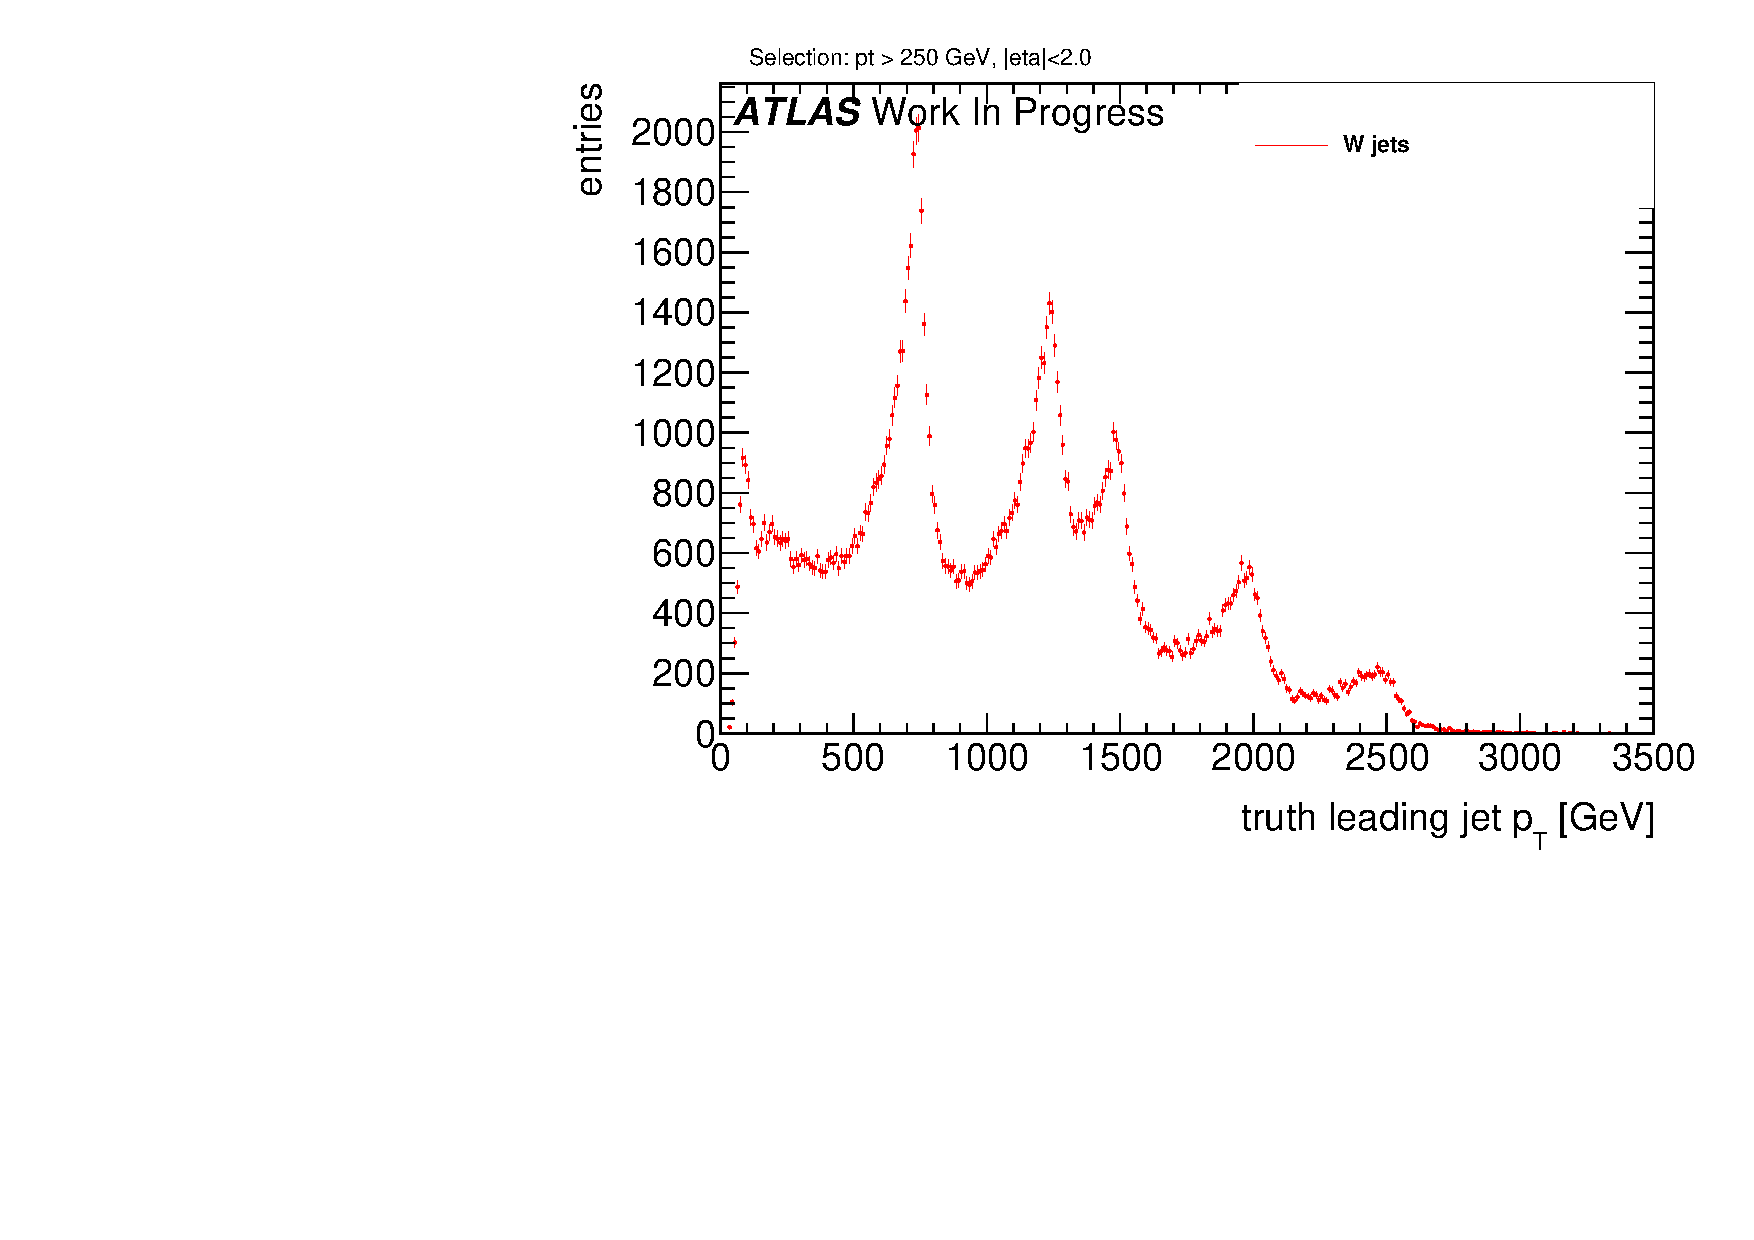
\includegraphics[width=0.5\textwidth]{sascha_input/plots/track_selection/h_leadpt_truth.pdf} \hspace{1mm}
	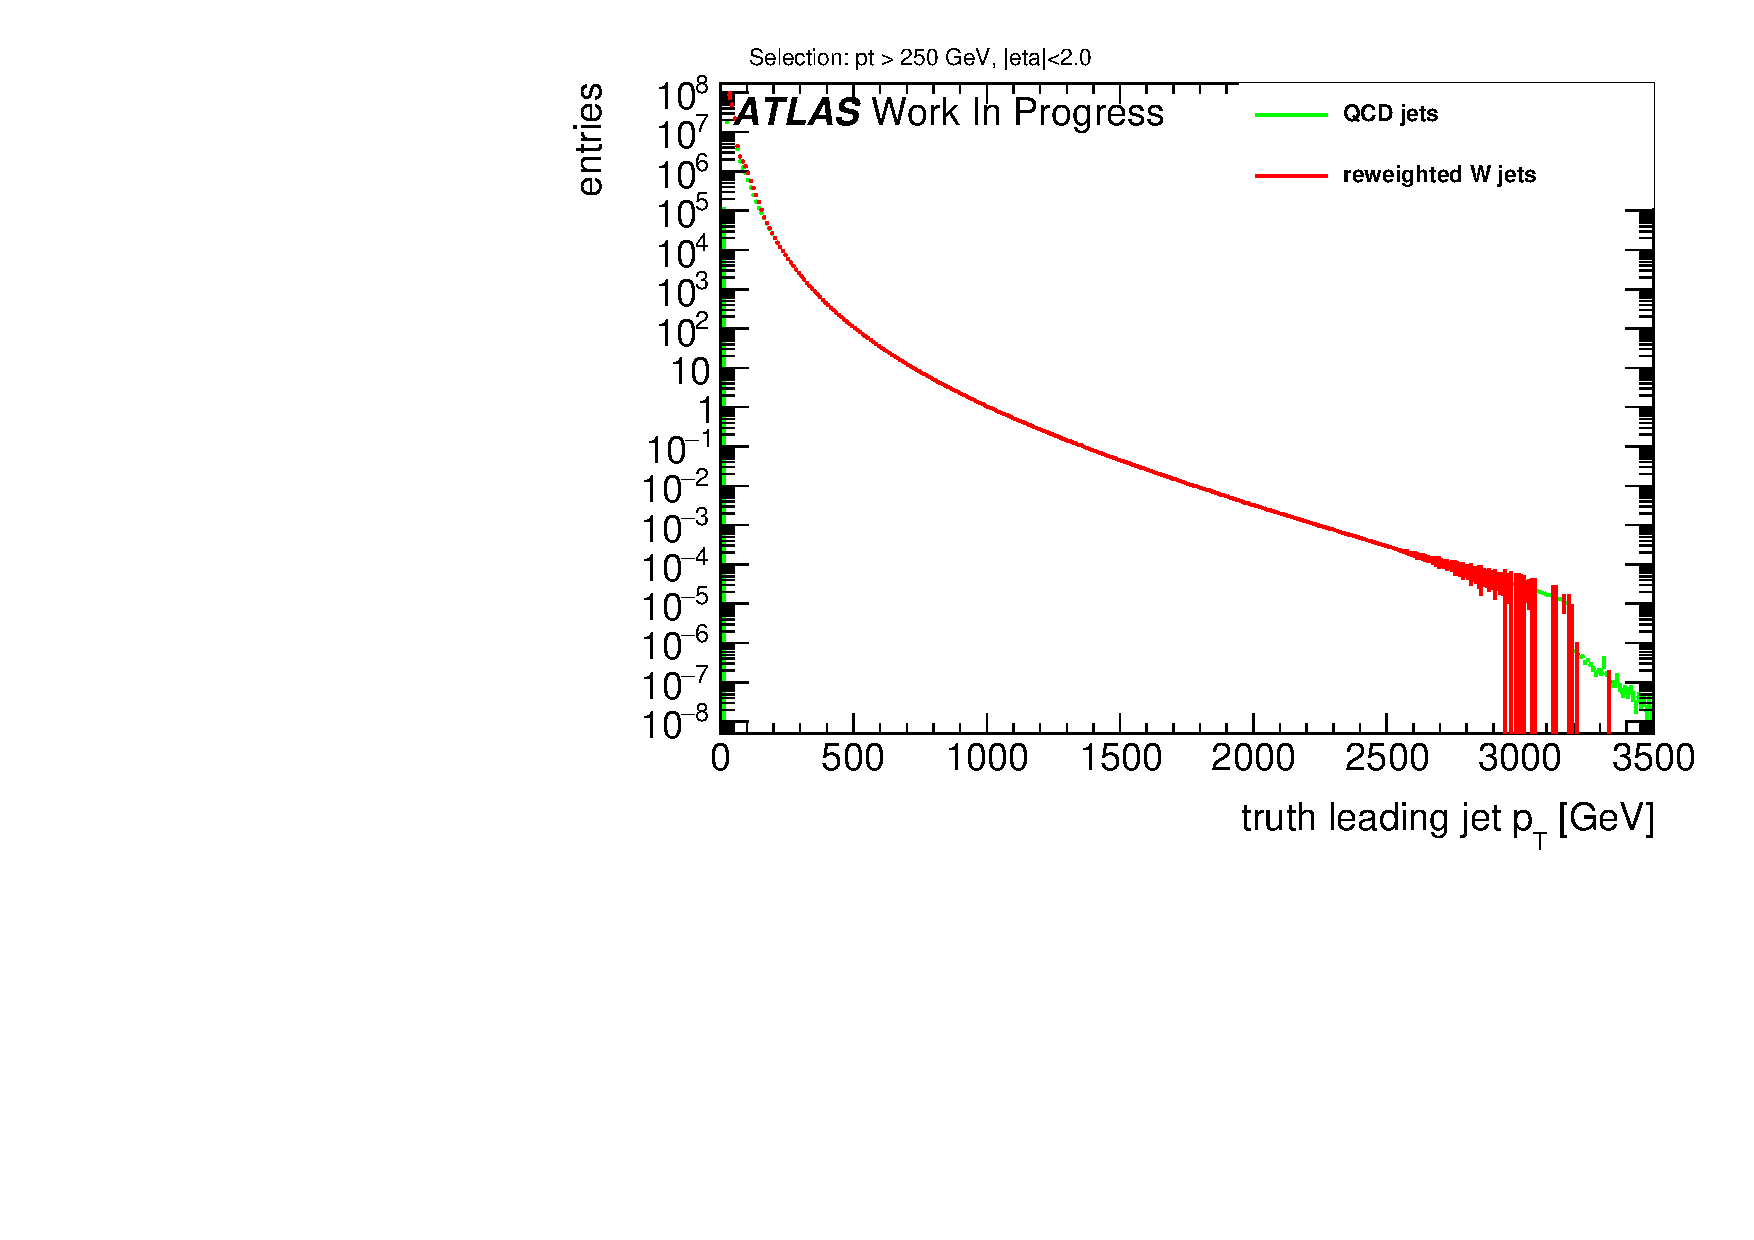
\includegraphics[width=0.5\textwidth]{sascha_input/plots/track_selection/h_leadpt_truth_weight.pdf}
\caption{{Exemplary $p_{\mathrm{T}}$ distributions of $W$ jets (left) and QCD jets from multi-jet events with reweighted $W$ boson events (right).}}\label{fig:p_T}
\end{figure}

\section{$p_{\text{T}}$ Dependence of Substructure Observables}\label{appendix:pt_dependence}
Due to the low weights for high $p_{\mathrm{T}}$, the correlation plots are divided into the six $p_{\mathrm{T}}$ regions. For C2, see Figure \ref{fig:correlation_C2}, observed is a strong trend to lower values (signal and background) for clusters and TAS. The TAS distributions concentrate at lower values compared to calorimeter counterparts.

For D2, Figure \ref{fig:correlation_D2}, and $\tau_{21}$, Figure \ref{fig:correlation_tau21}, there is a slight upward trend of the calorimeter variables in the lower $p_{\mathrm{T}}$ regions. With rising boost this slows down and ends in a broader distribution for $\tau_{21}$. This verifies the higher $p_{\mathrm{T}}$ dependence of the C2 variable in comparison to D2 and $\tau_{21}$. The TAS counterparts feature an even more robust signal with the background moving to higher values, hence improving separation. The $p_{\mathrm{T}}$ dependence of variables calculated with tracks is very similar to the ones with TAS, therefore they are omitted.
\begin{figure}[htp]
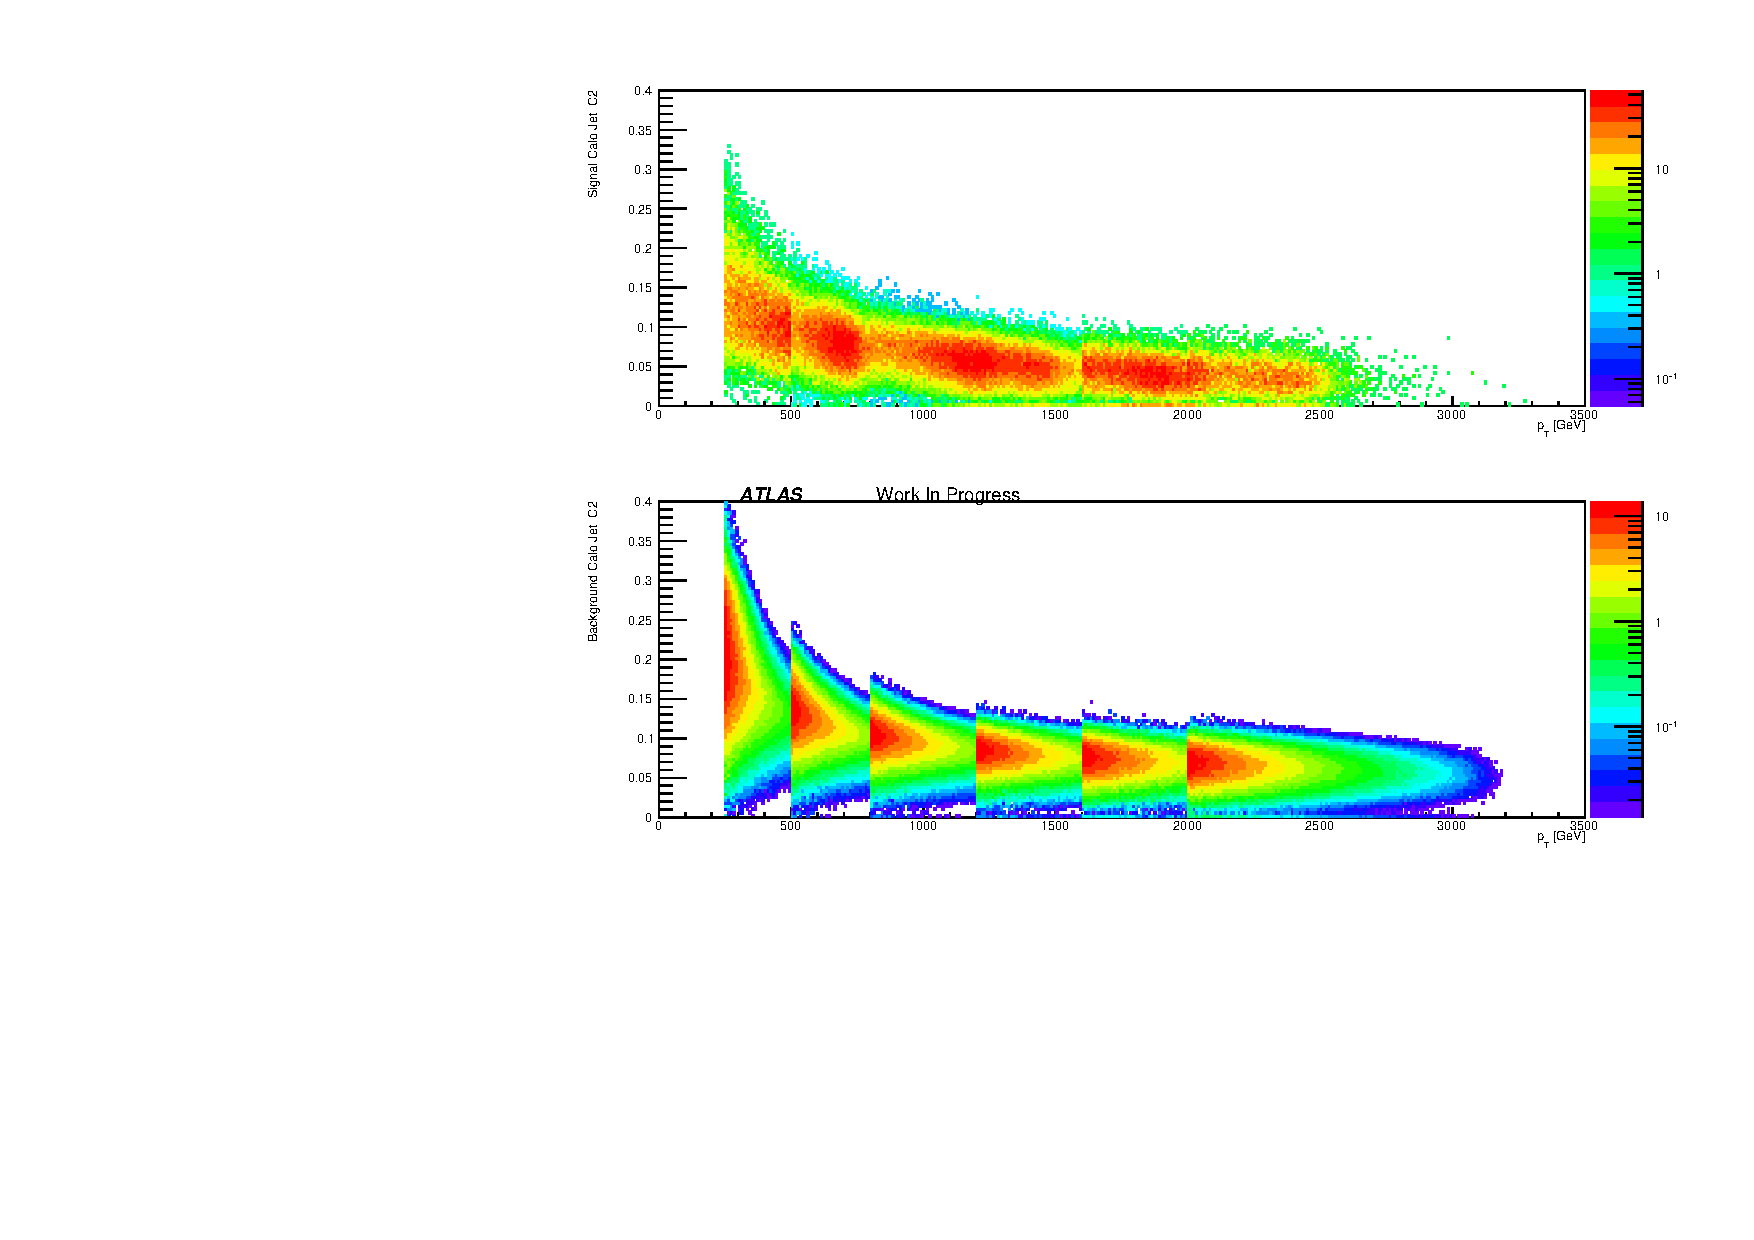
\includegraphics[width=0.5\textwidth]{sascha_input/plots/W/beta1/scatter_plots/scatter_h_scatter_reco_C2.pdf}
\bigskip
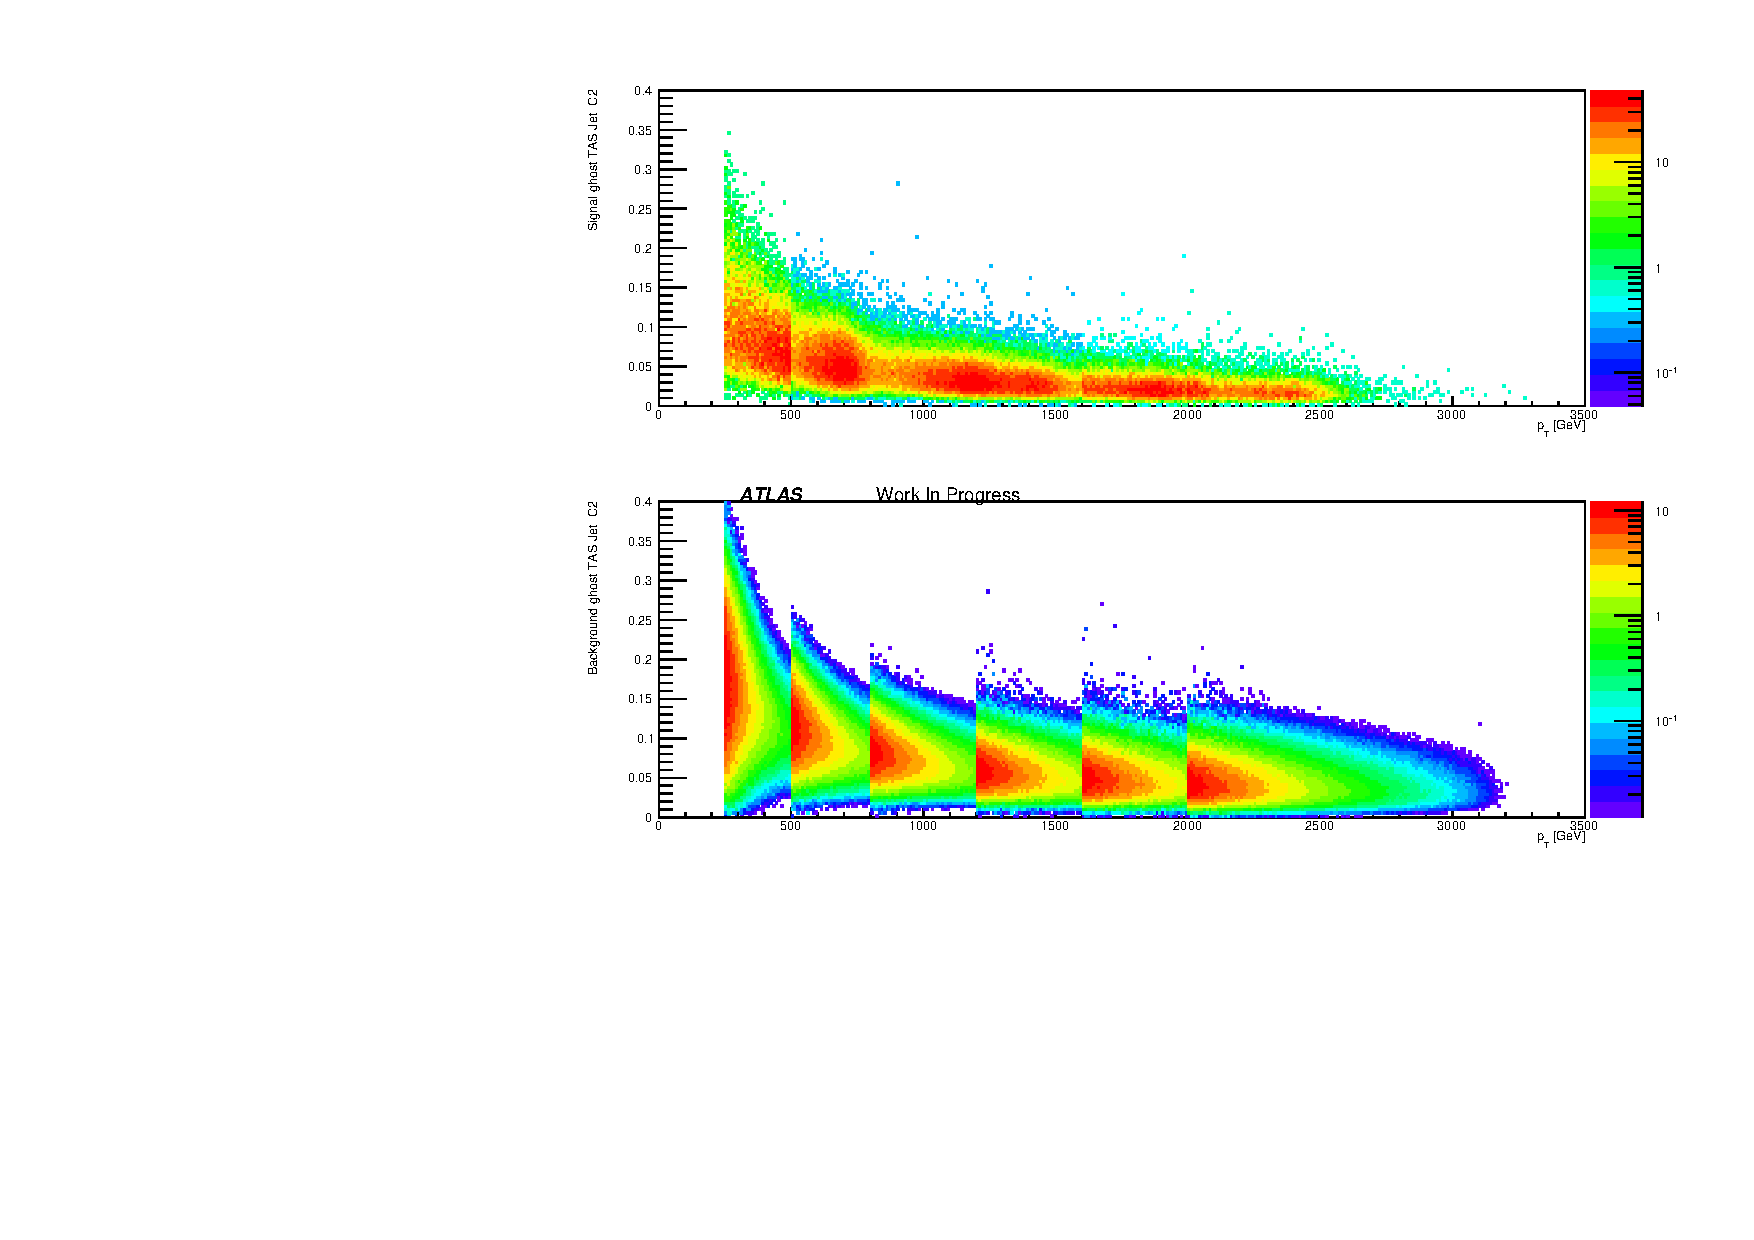
\includegraphics[width=0.5\textwidth]{sascha_input/plots/W/beta1/scatter_plots/scatter_h_scatter_assisted_tj_C2.pdf} 
\caption{{Correlation between C2 at $\beta=1$ and $p_{\mathrm{T}}$ applied on $W$ boson signal (above) and QCD background (below) for calorimeter (left) and TAS (right).}}\label{fig:correlation_C2}
\end{figure}
\begin{figure}[htp]
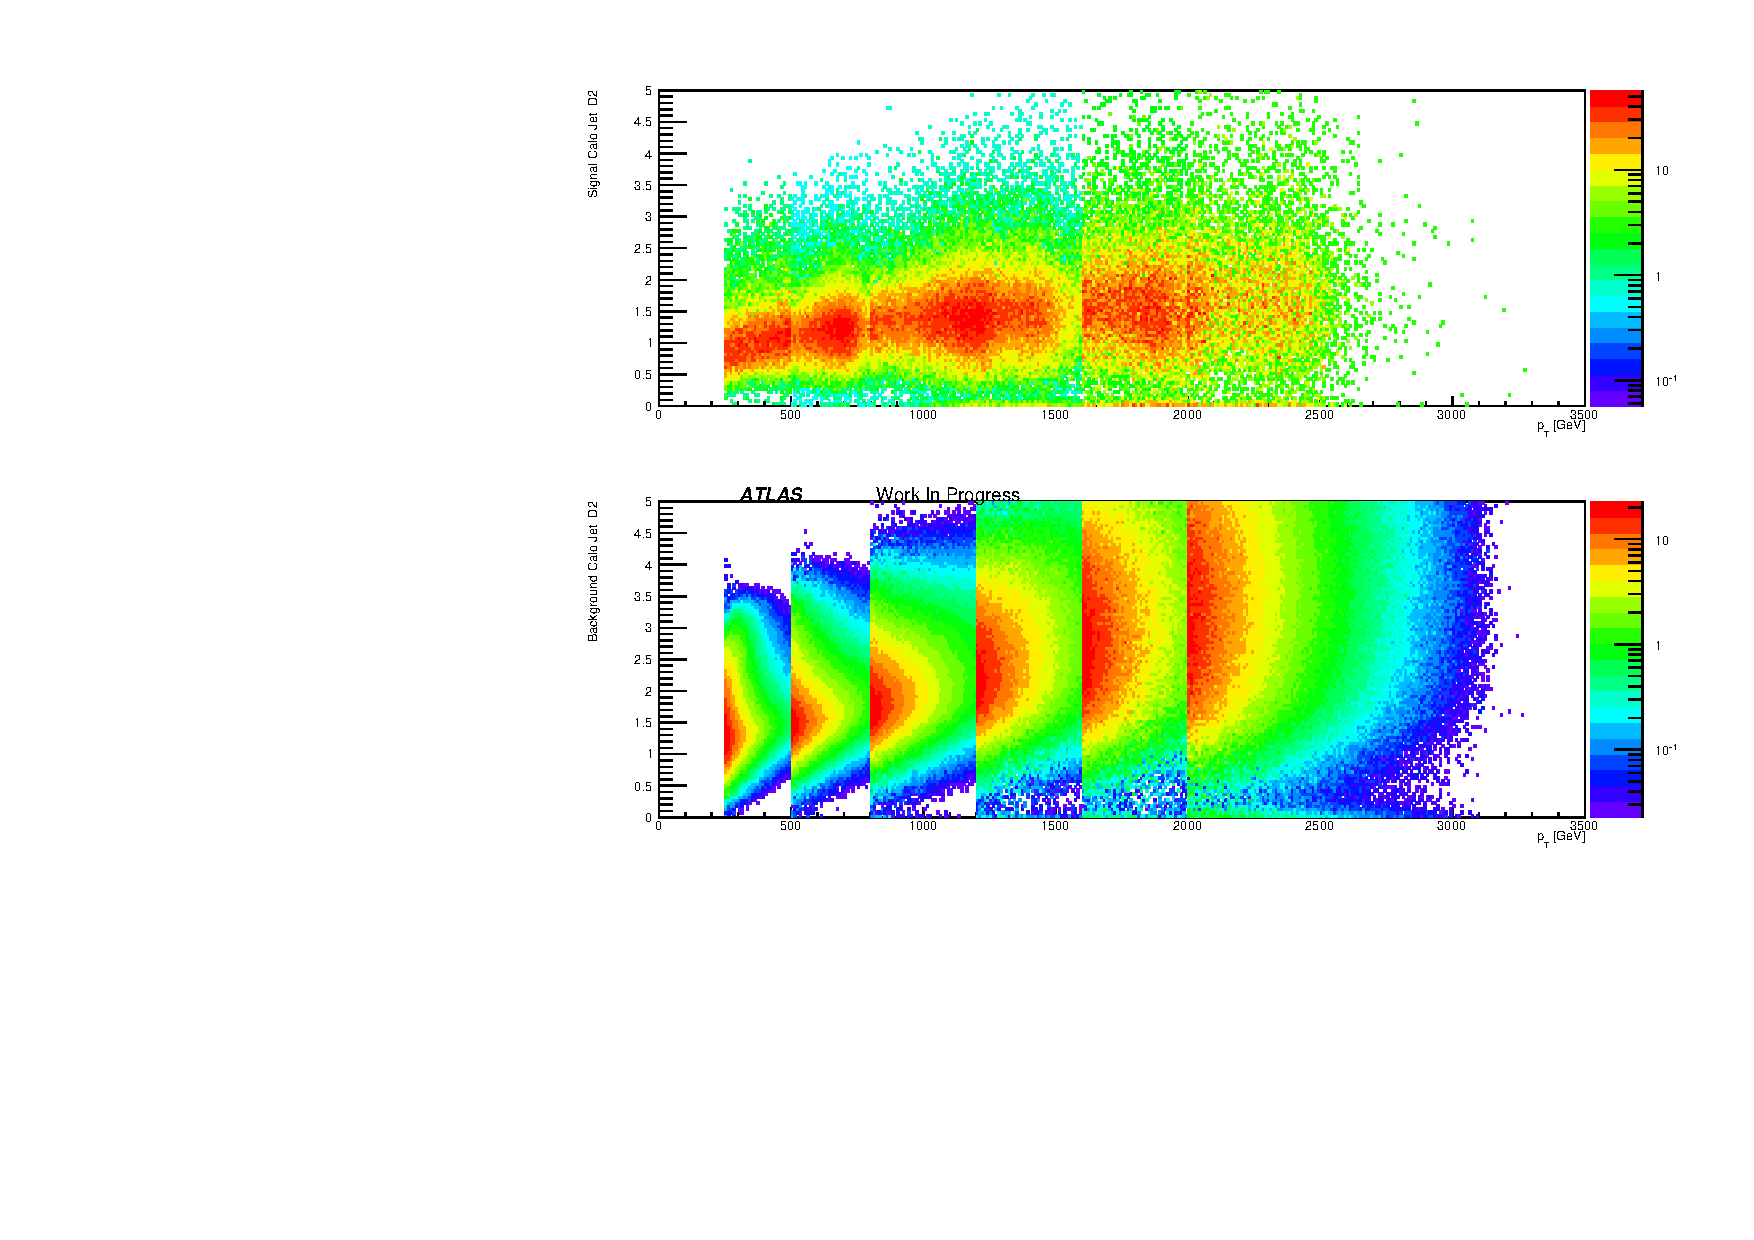
\includegraphics[width=0.5\textwidth]{sascha_input/plots/W/beta1/scatter_plots/scatter_h_scatter_reco_D2.pdf}
\bigskip
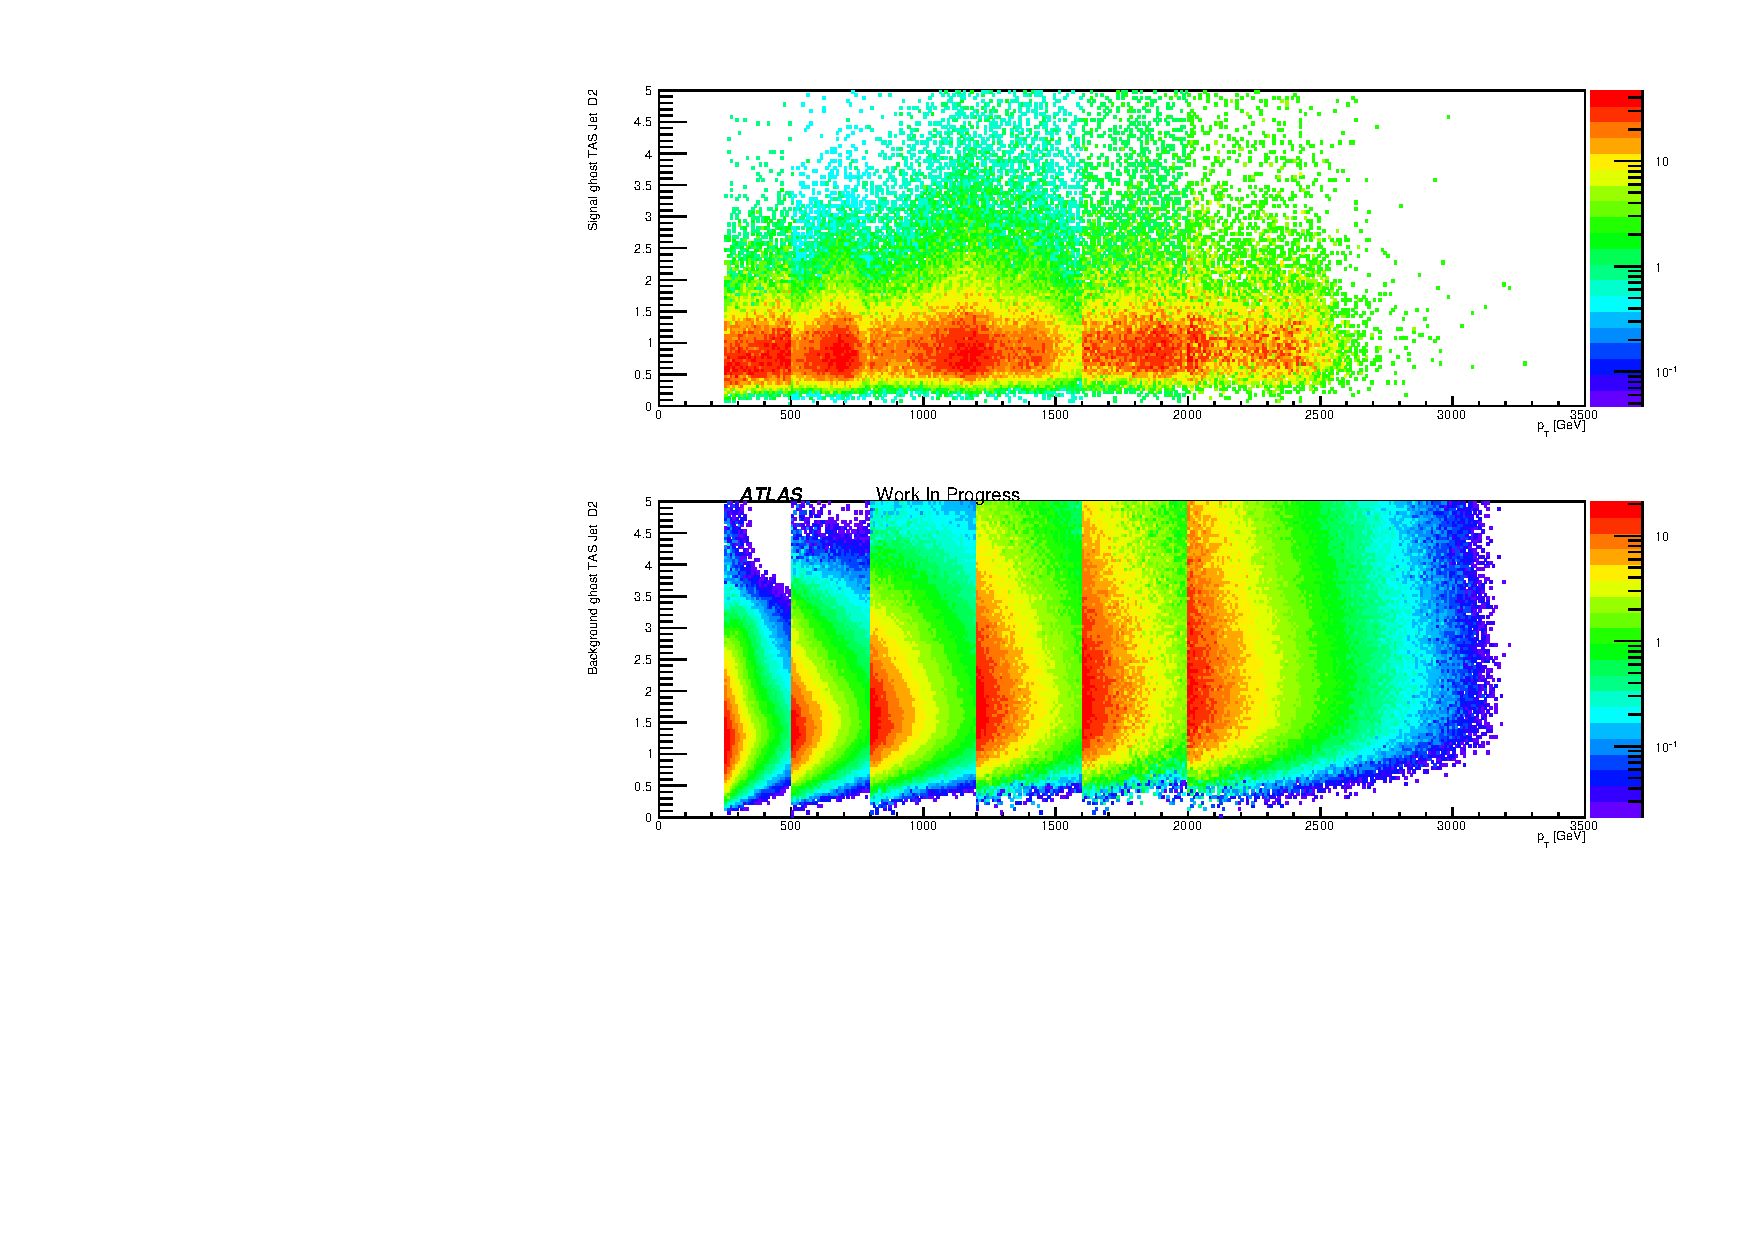
\includegraphics[width=0.5\textwidth]{sascha_input/plots/W/beta1/scatter_plots/scatter_h_scatter_assisted_tj_D2.pdf} 
\caption{{Correlation between D2 at $\beta=1$ and $p_{\mathrm{T}}$ applied on $W$ boson signal (above) and QCD background (below) for calorimeter (left) and TAS (right).}}\label{fig:correlation_D2}
\end{figure}
\begin{figure}[htp]
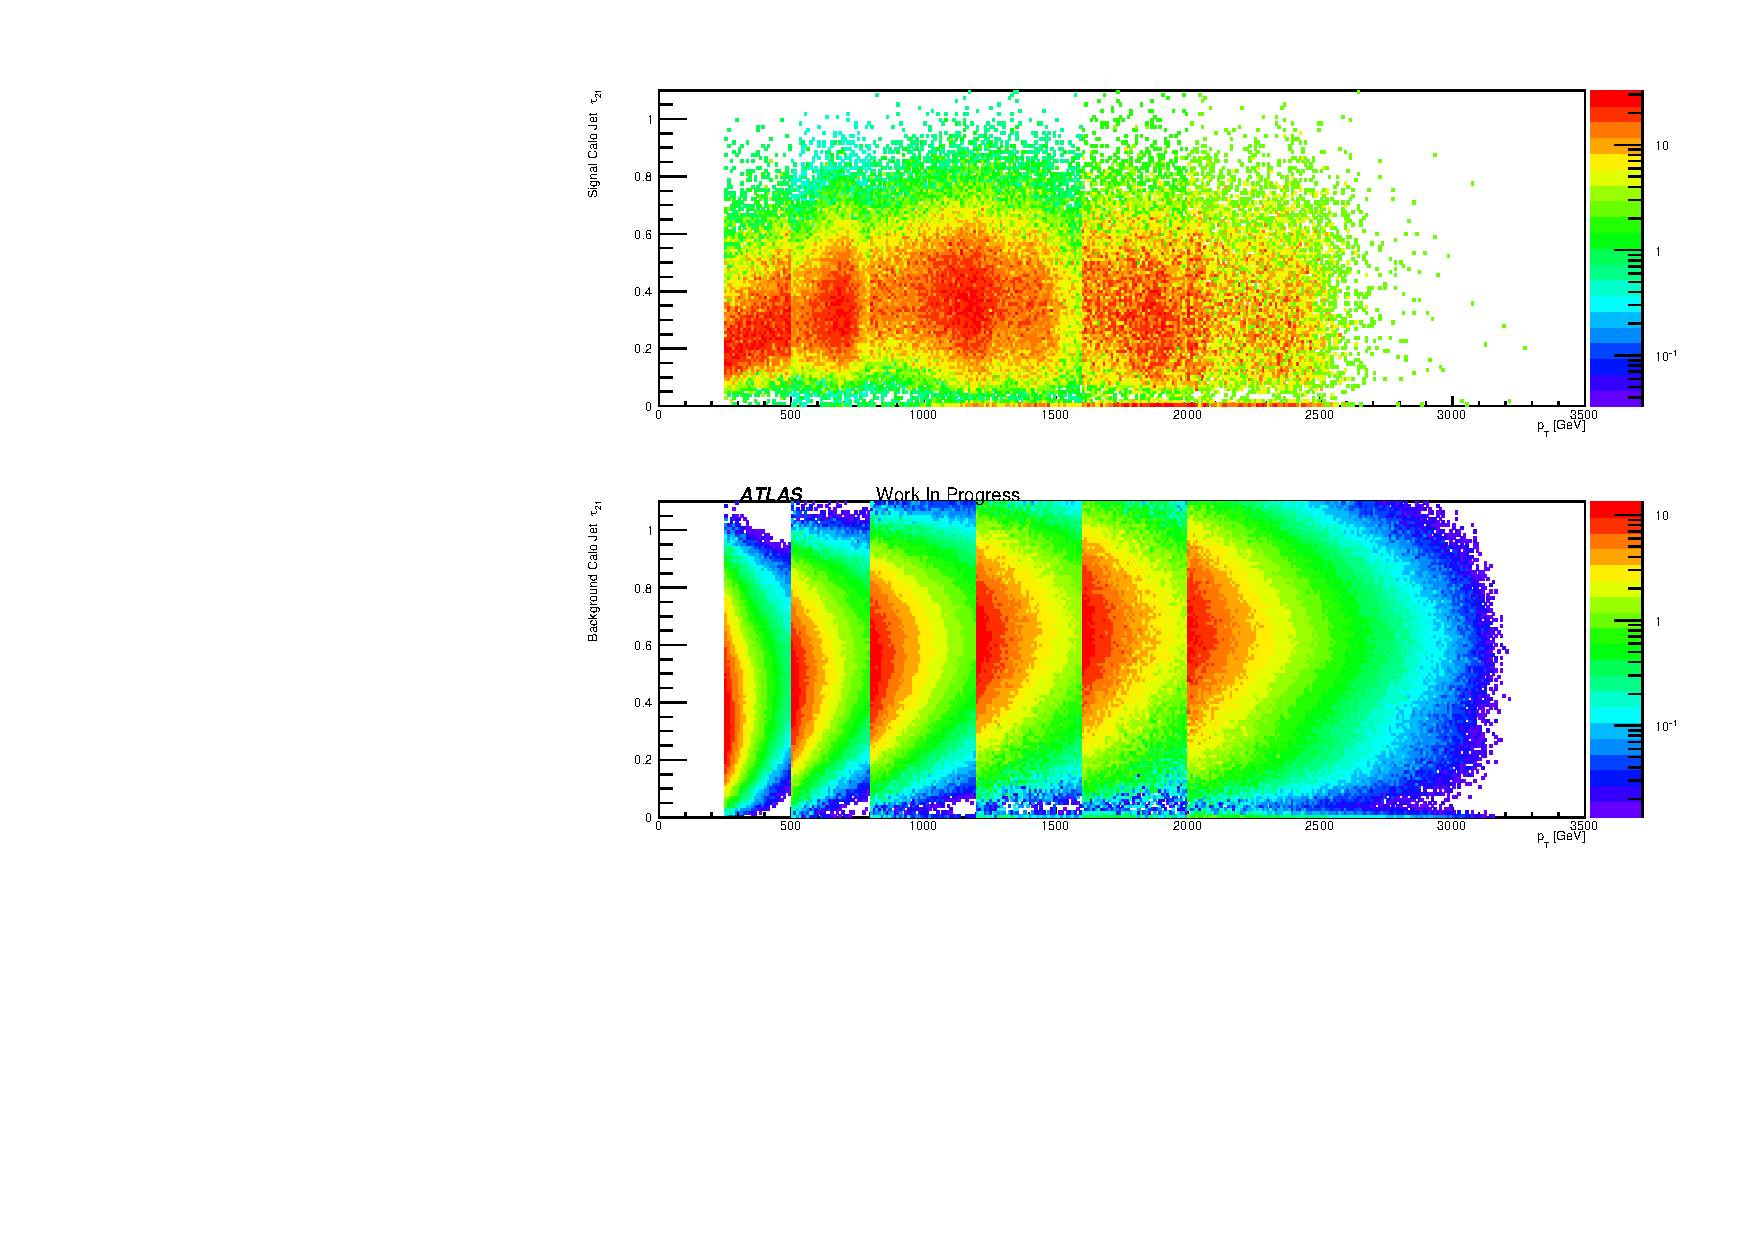
\includegraphics[width=0.5\textwidth]{sascha_input/plots/W/beta1/scatter_plots/scatter_h_scatter_reco_nSub21.pdf}
\bigskip
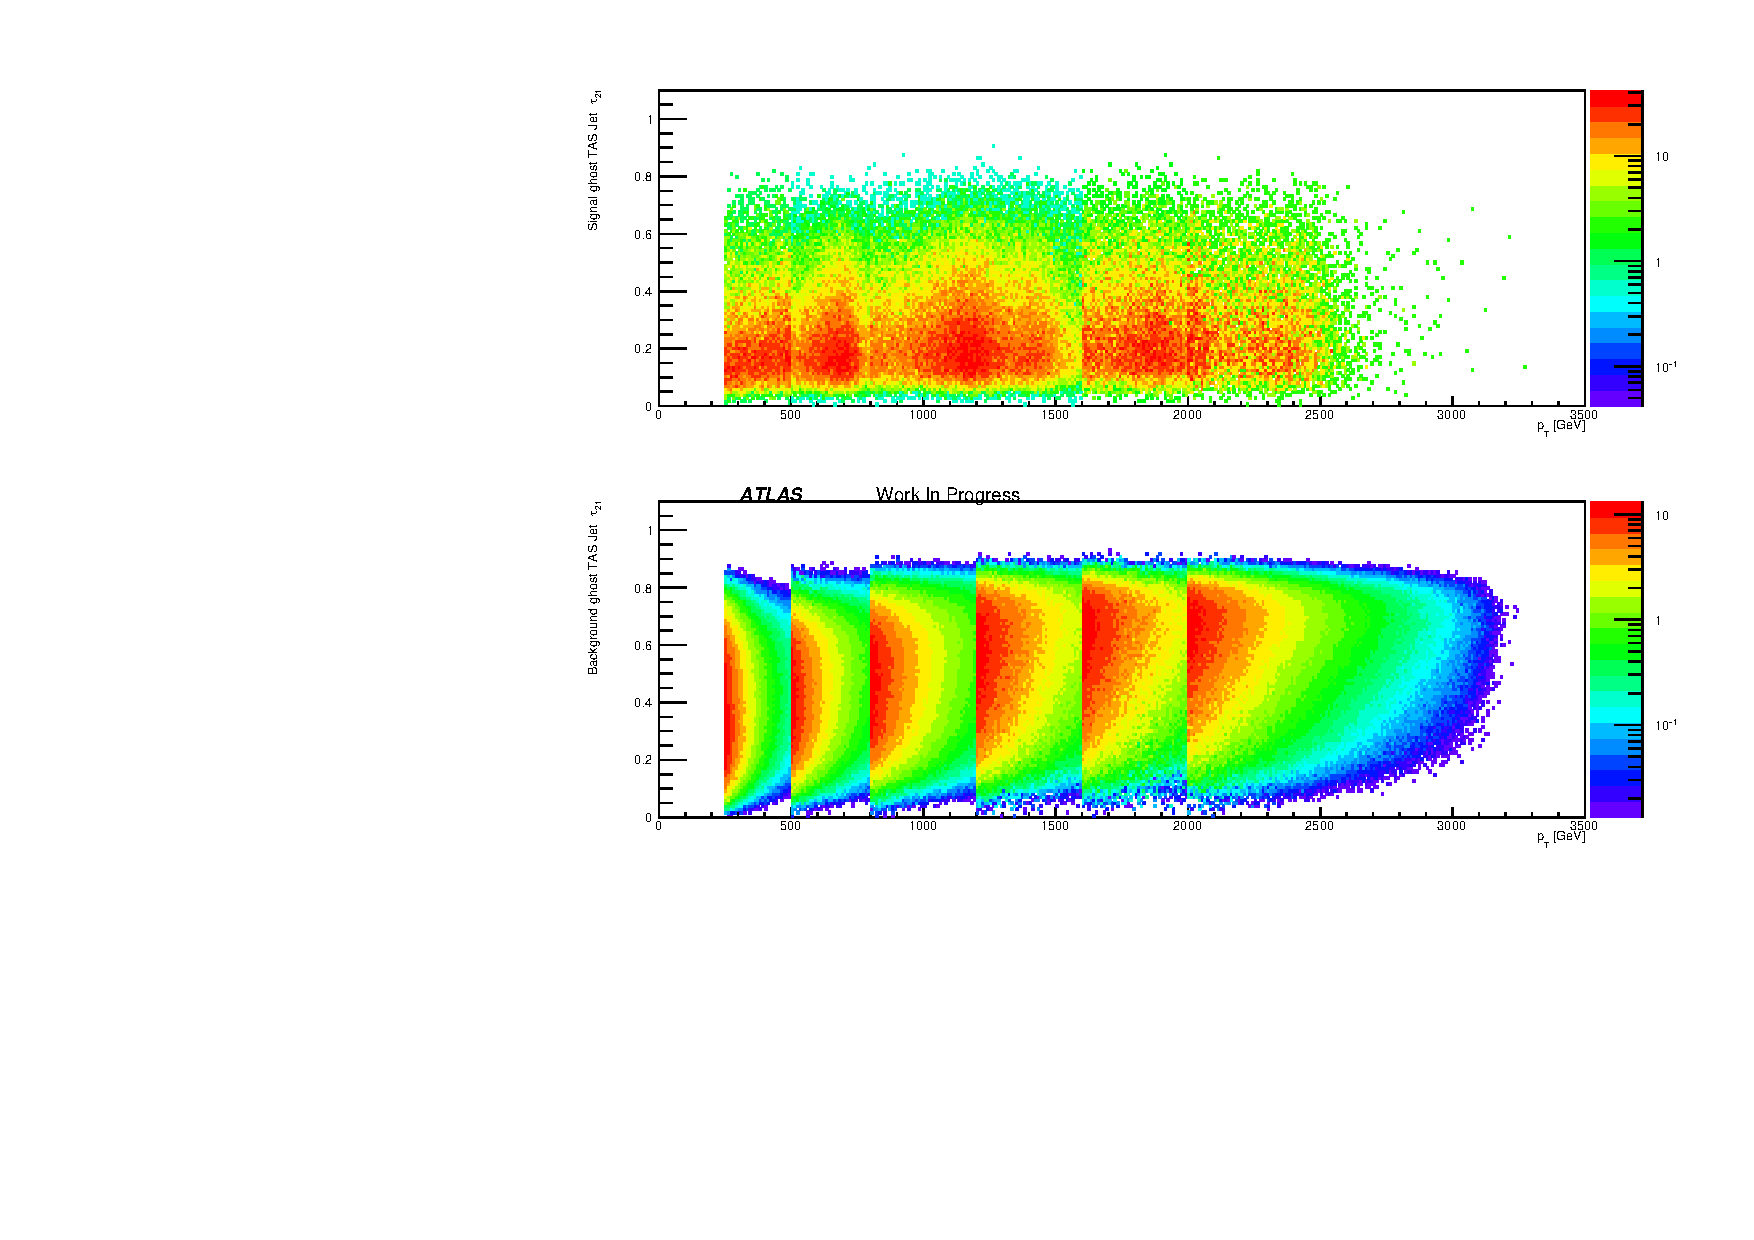
\includegraphics[width=0.5\textwidth]{sascha_input/plots/W/beta1/scatter_plots/scatter_h_scatter_assisted_tj_nSub21.pdf} 
\caption{{Correlation between $\tau_{21}$ at $\beta=1$ and $p_{\mathrm{T}}$ applied on $W$ boson signal (above) and QCD background (below) for calorimeter (left) and TAS (right).}}\label{fig:correlation_tau21}
\end{figure}

\section{Results of $\beta$ Optimisation}
\vspace{-0.25cm}
\subsection{Performance for $W$ tagging}\label{appendix:w_optimisation}
\vspace{-5cm}
\begin{sidewaystable}[htb]
\centering
\resizebox{22cm}{!}{%
\begin{tabular}{llllllllllllllll}
\rowcolor{Gray} \multicolumn{1}{l||}{\textbf{Calorimeter}} &  &  & C2 &  & \multicolumn{1}{l||}{} &  &  & D2 &  & \multicolumn{1}{l||}{} &  &  & $\tau_{21}$ &  & \multicolumn{1}{l|}{} \\ \hline
\multicolumn{1}{l||}{$p_{\mathrm{T}} \, \text{[GeV]}$} &  \multicolumn{1}{l|}{\cellcolor{Gray2}$\beta=0.5$} & \multicolumn{1}{l|}{\cellcolor{Gray2}1} & \multicolumn{1}{l|}{\cellcolor{Gray2}1.7} & \multicolumn{1}{l|}{\cellcolor{Gray2}2} & \multicolumn{1}{l||}{\cellcolor{Gray2}3} & \multicolumn{1}{l|}{\cellcolor{Gray2}$\beta=0.5$} & \multicolumn{1}{l|}{\cellcolor{Gray2}1} & \multicolumn{1}{l|}{\cellcolor{Gray2}1.7} & \multicolumn{1}{l|}{\cellcolor{Gray2}2} & \multicolumn{1}{l||}{\cellcolor{Gray2}3} & \multicolumn{1}{l|}{\cellcolor{Gray2}$\beta=0.5$} & \multicolumn{1}{l|}{\cellcolor{Gray2}1} & \multicolumn{1}{l|}{\cellcolor{Gray2}1.7} & \multicolumn{1}{l|}{\cellcolor{Gray2}2} & \multicolumn{1}{l|}{\cellcolor{Gray2}3} \\ \hline \hline
\multicolumn{1}{l||}{250 - 500} & 	\multicolumn{1}{l|}{29.7(1.5)} & 	 \multicolumn{1}{l|}{31.7(1.9)} & 		\multicolumn{1}{l|}{31.4(1.6)} & 	 \multicolumn{1}{l|}{30.7(1.9)} &     \multicolumn{1}{l||}{28.5(1.4)} & 	\multicolumn{1}{l|}{27.2(2.0)}& 	\multicolumn{1}{l|}{\cellcolor{Red!50}35.0(2.0)} & 		\multicolumn{1}{l|}{33.0(1.8)} & 		\multicolumn{1}{l|}{31.3(1.7)} & 	 \multicolumn{1}{l||}{25.7(1.2)} & 	   \multicolumn{1}{l|}{33.1(1.8)} & \multicolumn{1}{l|}{27.6(1.3)} & \multicolumn{1}{l|}{26.2(1.4)} & \multicolumn{1}{l|}{25.1(1.2)} & \multicolumn{1}{l|}{22.4(0.8)} \\
\multicolumn{1}{l||}{500 - 800} & 	\multicolumn{1}{l|}{44.2(1.8)} & 	 \multicolumn{1}{l|}{50.1(2.0)} & 		\multicolumn{1}{l|}{49.6(1.9)} & 	 \multicolumn{1}{l|}{48.6(1.8)} & 	  \multicolumn{1}{l||}{42.6(1.9)} &  	\multicolumn{1}{l|}{40.3(2.2)} & 	\multicolumn{1}{l|}{\cellcolor{Red!50}55.3(2.6)} & 		\multicolumn{1}{l|}{56.3(2.4)} & 		\multicolumn{1}{l|}{52.5(2.1)} & 	 \multicolumn{1}{l||}{39.3(1.3)} & 	   \multicolumn{1}{l|}{49.4(2.0)} & \multicolumn{1}{l|}{41.1(1.4)} & \multicolumn{1}{l|}{43.3(1.7)} & \multicolumn{1}{l|}{41.3(1.6)} & \multicolumn{1}{l|}{36.1(1.2)} \\
\multicolumn{1}{l||}{800 - 1200} & 	\multicolumn{1}{l|}{32.0(1.5)} & 	 \multicolumn{1}{l|}{37.5(1.7)} & 		\multicolumn{1}{l|}{35.4(1.5)} & 	 \multicolumn{1}{l|}{33.4(1.5)} & 	  \multicolumn{1}{l||}{26.8(0.9)} &  	\multicolumn{1}{l|}{34.0(2.1)} & 	\multicolumn{1}{l|}{\cellcolor{Red!50}41.1(2.0)} & 		\multicolumn{1}{l|}{38.5(1.6)} & 		\multicolumn{1}{l|}{34.9(1.3)} & 	 \multicolumn{1}{l||}{25.4(0.7)} & 	   \multicolumn{1}{l|}{30.5(1.2)} & \multicolumn{1}{l|}{30.9(1.2)} & \multicolumn{1}{l|}{33.8(1.4)} & \multicolumn{1}{l|}{32.5(1.3)} & \multicolumn{1}{l|}{28.1(0.9)} \\
\multicolumn{1}{l||}{1200 - 1600} & \multicolumn{1}{l|}{30.1(1.3)} & 	 \multicolumn{1}{l|}{34.4(1.8)} & 		\multicolumn{1}{l|}{29.4(1.3)} & 	 \multicolumn{1}{l|}{26.8(1.0)} & 	  \multicolumn{1}{l||}{20.7(0.8)} &  	\multicolumn{1}{l|}{34.1(1.8)} & 	\multicolumn{1}{l|}{\cellcolor{Red!50}38.1(1.9)} & 		\multicolumn{1}{l|}{31.4(1.4)} & 		\multicolumn{1}{l|}{27.6(1.2)} & 	 \multicolumn{1}{l||}{19.3(0.5)} & 	   \multicolumn{1}{l|}{23.1(0.9)} & \multicolumn{1}{l|}{27.3(1.)} & \multicolumn{1}{l|}{31.1(1.2)} & \multicolumn{1}{l|}{29.9(1.3)} & \multicolumn{1}{l|}{24.8(0.9)} \\
\multicolumn{1}{l||}{1600 - 2000} & \multicolumn{1}{l|}{20.9(1.3)} & 	 \multicolumn{1}{l|}{22.4(1.5)} & 		\multicolumn{1}{l|}{18.2(1.2)} & 	 \multicolumn{1}{l|}{16.5(0.9)} & 	  \multicolumn{1}{l||}{12.9(0.6)} &  	\multicolumn{1}{l|}{26.4(1.7)} & 	\multicolumn{1}{l|}{\cellcolor{Red!50}25.4(1.3)} & 		\multicolumn{1}{l|}{19.3(1.1)} & 		\multicolumn{1}{l|}{16.9(0.9)} & 	 \multicolumn{1}{l||}{11.9(0.5)} & 	   \multicolumn{1}{l|}{16.4(1.0)} & \multicolumn{1}{l|}{19.1(1.1)} & \multicolumn{1}{l|}{21.1(1.1)} & \multicolumn{1}{l|}{19.9(1.0)} & \multicolumn{1}{l|}{16.0(0.9)} \\
\multicolumn{1}{l||}{$>2000$} & 	\multicolumn{1}{l|}{16.9(1.4)} & 	 \multicolumn{1}{l|}{18.7(1.4)} & 		\multicolumn{1}{l|}{14.1(0.9)} & 	 \multicolumn{1}{l|}{12.6(0.8)} & 	  \multicolumn{1}{l||}{9.9(0.7)} & 		\multicolumn{1}{l|}{23.3(1.9)} & 	\multicolumn{1}{l|}{\cellcolor{Red!50}21.9(1.7)} & 		\multicolumn{1}{l|}{15.7(1.1)} & 		\multicolumn{1}{l|}{13.5(0.9)} & 	 \multicolumn{1}{l||}{9.2(0.4)} & 	   \multicolumn{1}{l|}{12.3(1.1)} & \multicolumn{1}{l|}{15.5(1.1)} & \multicolumn{1}{l|}{17.2(1.2)} & \multicolumn{1}{l|}{15.7(1.1)} & \multicolumn{1}{l|}{11.9(0.8)} \\ \hline
 &  &  &  &  &  &  &  &  &  &  &  &  &  &  &  \\
\rowcolor{Gray} \multicolumn{1}{l||}{\textbf{TAS}} &  &  & C2 &  & \multicolumn{1}{l||}{} &  &  & D2 &  & \multicolumn{1}{l||}{} &  &  & $\tau_{21}$ &  & \multicolumn{1}{l|}{} \\ \hline
\multicolumn{1}{l||}{$p_{\mathrm{T}} \, \text{[GeV]}$}   &  \multicolumn{1}{l|}{ \cellcolor{Gray2} $\beta=0.5$} & \multicolumn{1}{l|}{\cellcolor{Gray2} 1} & \multicolumn{1}{l|}{\cellcolor{Gray2}1.7} &   \multicolumn{1}{l|}{\cellcolor{Gray2} 2} &  \multicolumn{1}{l||}{\cellcolor{Gray2} 3} & \multicolumn{1}{l|}{\cellcolor{Gray2} $\beta=0.5$} &  \multicolumn{1}{l|}{\cellcolor{Gray2} 1} & 	\multicolumn{1}{l|}{\cellcolor{Gray2} 1.7} & 	\multicolumn{1}{l|}{\cellcolor{Gray2} 2} & \multicolumn{1}{l||}{\cellcolor{Gray2} 3} & \multicolumn{1}{l|}{ \cellcolor{Gray2} $\beta=0.5$} & \multicolumn{1}{l|}{\cellcolor{Gray2} 1} & \multicolumn{1}{l|}{\cellcolor{Gray2} 1.7} &  \multicolumn{1}{l|}{\cellcolor{Gray2} 2} & \multicolumn{1}{l|}{\cellcolor{Gray2} 3} \\ \hline \hline
\multicolumn{1}{l||}{250 - 500} & 	\multicolumn{1}{l|}{29.4(1.9)} & \multicolumn{1}{l|}{30.1(1.9)} & \multicolumn{1}{l|}{28.9(1.5)} & 				     	\multicolumn{1}{l|}{28.5(1.3)} & 						\multicolumn{1}{l||}{27.7(1.3)} & \multicolumn{1}{l|}{28.6(2.0)} & \multicolumn{1}{l|}{\cellcolor{Red!50}37.7(2.1)} & 		\multicolumn{1}{l|}{35.4(2.3)} & 					\multicolumn{1}{l|}{33.4(2.0)} & 	\multicolumn{1}{l||}{29.4(1.2)} & 					\multicolumn{1}{l|}{36.2(2.2)} & 	\multicolumn{1}{l|}{31.5(1.6)} & \multicolumn{1}{l|}{26.8(1.3)} & \multicolumn{1}{l|}{25.4(1.4)} & \multicolumn{1}{l|}{24.0(1.0)} \\
\multicolumn{1}{l||}{500 - 800} & 	\multicolumn{1}{l|}{48.2(2.0)} & \multicolumn{1}{l|}{55.5(2.7)} & \multicolumn{1}{l|}{58.6(2.6)} & 				     	\multicolumn{1}{l|}{59.1(2.7)} & 						\multicolumn{1}{l||}{56.8(2.0)} & \multicolumn{1}{l|}{42.8(2.3)} & \multicolumn{1}{l|}{67.2(3.1)} & 						\multicolumn{1}{l|}{\cellcolor{Red!50}67.6(3.2)} & 	\multicolumn{1}{l|}{63.7(3.0)} & 	\multicolumn{1}{l||}{52.6(2.3)} & 					\multicolumn{1}{l|}{55.7(2.6)} & 	\multicolumn{1}{l|}{51.9(2.1)} & \multicolumn{1}{l|}{45.5(2.0)} & \multicolumn{1}{l|}{44.0(1.9)} & \multicolumn{1}{l|}{41.3(1.5)} \\
\multicolumn{1}{l||}{800 - 1200} & 	\multicolumn{1}{l|}{31.0(1.2)} & \multicolumn{1}{l|}{44.6(1.9)} & \multicolumn{1}{l|}{54.6(2.8)} & 				     	\multicolumn{1}{l|}{\cellcolor{Red!50}55.2(2.8)} & 		\multicolumn{1}{l||}{53.0(3.2)} & \multicolumn{1}{l|}{26.1(1.3)} & \multicolumn{1}{l|}{47.6(2.3)} & 						\multicolumn{1}{l|}{54.9(2.4)} & 					\multicolumn{1}{l|}{52.6(2.8)} & 	\multicolumn{1}{l||}{43.1(1.5)} & 					\multicolumn{1}{l|}{36.4(1.8)} & 	\multicolumn{1}{l|}{37.3(1.7)} & \multicolumn{1}{l|}{36.2(1.8)} & \multicolumn{1}{l|}{36.2(1.6)} & \multicolumn{1}{l|}{35.5(1.6)} \\
\multicolumn{1}{l||}{1200 - 1600} & \multicolumn{1}{l|}{20.9(0.7)} & \multicolumn{1}{l|}{39.1(1.9)} & \multicolumn{1}{l|}{53.8(2.6)} & 				     	\multicolumn{1}{l|}{\cellcolor{Red!50}55.1(3.0)} & 		\multicolumn{1}{l||}{50.1(1.6)} & \multicolumn{1}{l|}{22.7(1.4)} & \multicolumn{1}{l|}{42.1(2.4)} & 						\multicolumn{1}{l|}{50.8(1.8)} & 					\multicolumn{1}{l|}{49.6(2.3)} & 	\multicolumn{1}{l||}{41.1(1.2)} & 					\multicolumn{1}{l|}{27.9(1.3)} & 	\multicolumn{1}{l|}{31.4(1.5)} & \multicolumn{1}{l|}{33.4(1.6)} & \multicolumn{1}{l|}{34.0(2.0)} & \multicolumn{1}{l|}{33.0(1.8)} \\
\multicolumn{1}{l||}{1600 - 2000} & \multicolumn{1}{l|}{16.7(0.7)} & \multicolumn{1}{l|}{36.9(2.9)} & \multicolumn{1}{l|}{\cellcolor{Red!50}50.9(4.3)} &    \multicolumn{1}{l|}{50.3(4.4)} & 						\multicolumn{1}{l||}{42.2(2.4)} & \multicolumn{1}{l|}{18.7(1.7)} & \multicolumn{1}{l|}{32.7(3.3)} & 						\multicolumn{1}{l|}{37.8(2.0)} & 					\multicolumn{1}{l|}{36.1(2.4)} & 	\multicolumn{1}{l||}{28.7(1.2)} & 					\multicolumn{1}{l|}{20.5(1.2)} & 	\multicolumn{1}{l|}{24.8(1.6)} & \multicolumn{1}{l|}{26.1(2.0)} & \multicolumn{1}{l|}{26.5(2.0)} & \multicolumn{1}{l|}{25.4(2.0)} \\
\multicolumn{1}{l||}{$>2000$} & 	\multicolumn{1}{l|}{11.6(0.6)} & \multicolumn{1}{l|}{31.2(3.2)} & \multicolumn{1}{l|}{\cellcolor{Red!50}46.1(4.7)} &    \multicolumn{1}{l|}{45.5(5.2)} & 						\multicolumn{1}{l||}{35.5(3.8)} & \multicolumn{1}{l|}{17.8(2.0)} & \multicolumn{1}{l|}{33.0(4.0)} & 						\multicolumn{1}{l|}{36.3(2.0)} & 					\multicolumn{1}{l|}{34.0(2.5)} & 	\multicolumn{1}{l||}{27.4(1.3)} & 					\multicolumn{1}{l|}{16.4(1.3)} & 	\multicolumn{1}{l|}{22.3(2.0)} & \multicolumn{1}{l|}{24.2(2.2)} & \multicolumn{1}{l|}{24.4(2.5)} & \multicolumn{1}{l|}{21.8(2.4)} \\ \hline
 &  &  &  &  &  &  &  &  &  &  &  &  &  &  &  \\
\rowcolor{Gray} \multicolumn{1}{l||}{\textbf{Tracks}} &  &  & C2 &  & \multicolumn{1}{l||}{} &  &  & D2 &  & \multicolumn{1}{l||}{} &  &  & $\tau_{21}$ &  & \multicolumn{1}{l|}{} \\ \hline
\multicolumn{1}{l||}{$p_{\mathrm{T}} \, \text{[GeV]}$}  & \multicolumn{1}{l|}{\cellcolor{Gray2}$\beta=0.5$} & \multicolumn{1}{l|}{\cellcolor{Gray2}1} & \multicolumn{1}{l|}{\cellcolor{Gray2}1.7} & \multicolumn{1}{l|}{\cellcolor{Gray2}2} & \multicolumn{1}{l||}{\cellcolor{Gray2}3} & \multicolumn{1}{l|}{\cellcolor{Gray2}$\beta=0.5$} & \multicolumn{1}{l|}{\cellcolor{Gray2}1} & \multicolumn{1}{l|}{\cellcolor{Gray2}1.7} & \multicolumn{1}{l|}{\cellcolor{Gray2}2} & \multicolumn{1}{l||}{\cellcolor{Gray2}3} & \multicolumn{1}{l|}{\cellcolor{Gray2}$\beta=0.5$} & \multicolumn{1}{l|}{\cellcolor{Gray2}1} & \multicolumn{1}{l|}{\cellcolor{Gray2}1.7} & \multicolumn{1}{l|}{\cellcolor{Gray2}2} & \multicolumn{1}{l|}{\cellcolor{Gray2}3} \\ \hline \hline
\multicolumn{1}{l||}{250 - 500} & 	\multicolumn{1}{l|}{27.1(1.2)} & \multicolumn{1}{l|}{28.1(1.5)} & \multicolumn{1}{l|}{28.7(1.9)} 						& \multicolumn{1}{l|}{28.7(1.9)} 					& \multicolumn{1}{l||}{28.2(1.7)} & \multicolumn{1}{l|}{21.6(1.2)} & \multicolumn{1}{l|}{28.9(2.0)} & \multicolumn{1}{l|}{\cellcolor{Red!50}29.5(1.8)} 		& \multicolumn{1}{l|}{29.1(1.6)} & \multicolumn{1}{l||}{28.1(1.3)} & \multicolumn{1}{l|}{28.7(1.8)} & \multicolumn{1}{l|}{28.0(1.7)} & \multicolumn{1}{l|}{25.6(1.3)} & \multicolumn{1}{l|}{25.1(1.3)} & \multicolumn{1}{l|}{24.2(0.9)} \\
\multicolumn{1}{l||}{500 - 800} & 	\multicolumn{1}{l|}{46.5(1.9)} & \multicolumn{1}{l|}{52.9(2.4)} & \multicolumn{1}{l|}{57.7(2.6)} 						& \multicolumn{1}{l|}{\cellcolor{Red!50}58.1(2.7)} 	& \multicolumn{1}{l||}{55.8(2.5)} & \multicolumn{1}{l|}{30.1(1.8)} & \multicolumn{1}{l|}{46.8(2.4)} & \multicolumn{1}{l|}{53.4(2.2)} 						& \multicolumn{1}{l|}{52.1(2.3)} & \multicolumn{1}{l||}{46.6(1.7)} & \multicolumn{1}{l|}{46.1(2.3)} & \multicolumn{1}{l|}{44.9(1.8)} & \multicolumn{1}{l|}{41.7(2.1)} & \multicolumn{1}{l|}{40.6(1.8)} & \multicolumn{1}{l|}{39.2(1.5)} \\
\multicolumn{1}{l||}{800 - 1200} & 	\multicolumn{1}{l|}{30.3(1.1)} & \multicolumn{1}{l|}{44.5(2.2)} & \multicolumn{1}{l|}{54.8(2.8)} 						& \multicolumn{1}{l|}{\cellcolor{Red!50}56.4(3.0)} 	& \multicolumn{1}{l||}{53.7(3.6)} & \multicolumn{1}{l|}{24.5(1.5)} & \multicolumn{1}{l|}{42.3(2.3)} & \multicolumn{1}{l|}{48.6(2.5)} 						& \multicolumn{1}{l|}{47.5(1.2)} & \multicolumn{1}{l||}{42.4(1.2)} & \multicolumn{1}{l|}{34.5(1.6)} & \multicolumn{1}{l|}{36.2(1.8)} & \multicolumn{1}{l|}{36.0(1.8)} & \multicolumn{1}{l|}{36.2(1.8)} & \multicolumn{1}{l|}{35.7(1.5)} \\
\multicolumn{1}{l||}{1200 - 1600} & \multicolumn{1}{l|}{20.7(0.6)} & \multicolumn{1}{l|}{39.0(1.9)} & \multicolumn{1}{l|}{54.2(2.7)} 						& \multicolumn{1}{l|}{\cellcolor{Red!50}55.5(3.3)} 	& \multicolumn{1}{l||}{50.9(1.7)} & \multicolumn{1}{l|}{22.7(1.3)} & \multicolumn{1}{l|}{41.0(2.2)} & \multicolumn{1}{l|}{50.0(1.6)} 						& \multicolumn{1}{l|}{47.6(2.2)} & \multicolumn{1}{l||}{41.4(1.2)} & \multicolumn{1}{l|}{27.7(1.2)} & \multicolumn{1}{l|}{31.3(1.4)} & \multicolumn{1}{l|}{33.3(1.6)} & \multicolumn{1}{l|}{33.9(1.7)} & \multicolumn{1}{l|}{33.2(1.8)} \\
\multicolumn{1}{l||}{1600 - 2000} & \multicolumn{1}{l|}{16.6(0.7)} & \multicolumn{1}{l|}{36.7(2.3)} & \multicolumn{1}{l|}{\cellcolor{Red!50}51.7(5.2)} 		& \multicolumn{1}{l|}{51.6(4.0)} 					& \multicolumn{1}{l||}{43.1(2.3)} & \multicolumn{1}{l|}{18.5(1.7)} & \multicolumn{1}{l|}{32.1(3.0)} & \multicolumn{1}{l|}{37.0(1.9)} 						& \multicolumn{1}{l|}{35.9(2.3)} & \multicolumn{1}{l||}{29.3(1.2)} & \multicolumn{1}{l|}{20.5(1.3)} & \multicolumn{1}{l|}{24.6(1.7)} & \multicolumn{1}{l|}{26.2(1.8)} & \multicolumn{1}{l|}{26.7(2.0)} & \multicolumn{1}{l|}{25.9(2.2)} \\
\multicolumn{1}{l||}{$>2000$} & 	\multicolumn{1}{l|}{11.6(0.5)} & \multicolumn{1}{l|}{31.5(3.0)} & \multicolumn{1}{l|}{\cellcolor{Red!50}46.8(5.7)} 		& \multicolumn{1}{l|}{46.0(4.2)} 					& \multicolumn{1}{l||}{36.1(4.3)} & \multicolumn{1}{l|}{17.8(2.2)} & \multicolumn{1}{l|}{33.0(3.3)} & \multicolumn{1}{l|}{35.9(2.1)} 						& \multicolumn{1}{l|}{34.2(2.6)} & \multicolumn{1}{l||}{28.1(1.0)} & \multicolumn{1}{l|}{16.4(1.4)} & \multicolumn{1}{l|}{22.5(1.8)} & \multicolumn{1}{l|}{24.5(2.4)} & \multicolumn{1}{l|}{24.7(2.6)} & \multicolumn{1}{l|}{22.2(2.6)} \\ \hline
\end{tabular}}
\caption{Listing of the QCD rejection for $W$ jets achieved with C2, D2 and $\tau_{21}$ calculated with varying angular weightings $\beta$ and constituents. The highest achieved background rejection per energy range is highlighted in red.}\label{table:w_scan}
\end{sidewaystable}

\FloatBarrier
\subsection{Performance for Higgs tagging}\label{appendix:higgs_optimisation}
\begin{sidewaystable}[h]
\centering
\hspace{-1cm}
\resizebox{22cm}{!}{%
\begin{tabular}{llllllllllllllll}
\rowcolor{Gray} \multicolumn{1}{l||}{\textbf{Calorimeter}}    &                                  &                           & C2                        &                           & \multicolumn{1}{l|}{}     &                                  &                           & D2                        &                           & \multicolumn{1}{l|}{}     &                                  &                           & $\tau_{21}$               &                           & \multicolumn{1}{l|}{}     \\ \hline
\multicolumn{1}{l||}{$p_{\mathrm{T}} \, [GeV]$} & \multicolumn{1}{l|}{\cellcolor{Gray2}$\beta=0.5$} & \multicolumn{1}{l|}{\cellcolor{Gray2}1}    & \multicolumn{1}{l|}{\cellcolor{Gray2}1.7}  & \multicolumn{1}{l|}{\cellcolor{Gray2}2}    & \multicolumn{1}{l||}{\cellcolor{Gray2}3}    & \multicolumn{1}{l|}{\cellcolor{Gray2}$\beta=0.5$} & \multicolumn{1}{l|}{\cellcolor{Gray2}1}    & \multicolumn{1}{l|}{\cellcolor{Gray2}1.7}  & \multicolumn{1}{l|}{\cellcolor{Gray2}2}    & \multicolumn{1}{l||}{\cellcolor{Gray2}3}    & \multicolumn{1}{l|}{\cellcolor{Gray2}$\beta=0.5$} & \multicolumn{1}{l|}{\cellcolor{Gray2}1}    & \multicolumn{1}{l|}{\cellcolor{Gray2}1.7}  & \multicolumn{1}{l|}{\cellcolor{Gray2}2}    & \multicolumn{1}{l|}{\cellcolor{Gray2}3}    \\ \hline \hline
\multicolumn{1}{l||}{250 - 500}      & \multicolumn{1}{l|}{4.6(0.1)}         & \multicolumn{1}{l|}{5.0(0.1)} & \multicolumn{1}{l|}{5.2(0.1)}  	    & \multicolumn{1}{l|}{5.3(0.1)}  & \multicolumn{1}{l||}{5.5(0.1)}  		& \multicolumn{1}{l|}{5.7(0.1)}         & \multicolumn{1}{l|}{7.3(0.2)}  & \multicolumn{1}{l|}{\cellcolor{Red!50}8.4(0.2)}  							& \multicolumn{1}{l|}{\cellcolor{Red!50}8.4(0.2)}  	    & \multicolumn{1}{l||}{\cellcolor{Red!50}8.4(0.2)}  & \multicolumn{1}{l|}{7.6(0.2)}         & \multicolumn{1}{l|}{8.0(0.2)}  & \multicolumn{1}{l|}{7.9(0.2)}  & \multicolumn{1}{l|}{7.8(0.2)}  & \multicolumn{1}{l|}{7.5(0.2)}  \\
\multicolumn{1}{l||}{500 - 800}      & \multicolumn{1}{l|}{15.7(0.3)}        & \multicolumn{1}{l|}{16.7(0.4)} & \multicolumn{1}{l|}{17.0(0.4)} 		& \multicolumn{1}{l|}{16.9(0.4)} & \multicolumn{1}{l||}{16.2(0.4)} 		& \multicolumn{1}{l|}{13.6(0.3)}        & \multicolumn{1}{l|}{16.9(0.4)} & \multicolumn{1}{l|}{\cellcolor{Red!50}17.7(0.4)} 		& \multicolumn{1}{l|}{17.2(0.4)} 						& \multicolumn{1}{l||}{15.2(0.3)} & \multicolumn{1}{l|}{16.7(0.4)}        & \multicolumn{1}{l|}{15.4(0.3)} & \multicolumn{1}{l|}{15.2(0.3)} & \multicolumn{1}{l|}{14.8(0.3)} & \multicolumn{1}{l|}{14.0(0.3)} \\
\multicolumn{1}{l||}{800 - 1200}     & \multicolumn{1}{l|}{22.1(0.5)}        & \multicolumn{1}{l|}{23.8(0.5)} & \multicolumn{1}{l|}{25.0(0.6)} 		& \multicolumn{1}{l|}{25.0(0.6)} & \multicolumn{1}{l||}{23.4(0.5)} 		& \multicolumn{1}{l|}{18.4(0.4)}        & \multicolumn{1}{l|}{23.7(0.6)} & \multicolumn{1}{l|}{\cellcolor{Red!50}26.3(0.6)} 							& \multicolumn{1}{l|}{25.6(0.6)} 		& \multicolumn{1}{l||}{22.3(0.5)} & \multicolumn{1}{l|}{22.8(0.5)}        & \multicolumn{1}{l|}{21.9(0.5)} & \multicolumn{1}{l|}{22.6(0.5)} & \multicolumn{1}{l|}{22.1(0.5)} & \multicolumn{1}{l|}{20.9(0.5)} \\
\multicolumn{1}{l||}{1200 - 1600}    & \multicolumn{1}{l|}{24.0(0.6)}        & \multicolumn{1}{l|}{26.0(0.8)} & \multicolumn{1}{l|}{26.4(0.8)} 		& \multicolumn{1}{l|}{25.9(0.7)} & \multicolumn{1}{l||}{23.0(0.6)} 		& \multicolumn{1}{l|}{19.3(0.6)}        & \multicolumn{1}{l|}{24.9(0.7)} & \multicolumn{1}{l|}{\cellcolor{Red!50}27.0(0.8)} 		& \multicolumn{1}{l|}{26.1(0.7)} 						& \multicolumn{1}{l||}{21.9(0.5)} & \multicolumn{1}{l|}{21.3(0.5)}        & \multicolumn{1}{l|}{22.6(0.6)} & \multicolumn{1}{l|}{24.0(0.6)} & \multicolumn{1}{l|}{23.7(0.6)} & \multicolumn{1}{l|}{22.2(0.5)} \\
\multicolumn{1}{l||}{1600 - 2000}    & \multicolumn{1}{l|}{12.1(0.7)}        & \multicolumn{1}{l|}{13.9(0.8)} & \multicolumn{1}{l|}{14.3(0.7)}  	& \multicolumn{1}{l|}{14.0(0.7)} & \multicolumn{1}{l||}{12.3(0.6)} 		& \multicolumn{1}{l|}{11.1(0.7)}        & \multicolumn{1}{l|}{14.1(0.9)} & \multicolumn{1}{l|}{\cellcolor{Red!50}14.9(0.8)} 		& \multicolumn{1}{l|}{14.2(0.6)} 						& \multicolumn{1}{l||}{11.8(0.5)} & \multicolumn{1}{l|}{10.3(0.5)}        & \multicolumn{1}{l|}{11.9(0.5)} & \multicolumn{1}{l|}{13.1(0.6)} & \multicolumn{1}{l|}{13.1(0.7)} & \multicolumn{1}{l|}{12.3(0.7)} \\ \hline
                                    &                                  &                           &                           &                	           &                           &                                  &                           &                           &                           &                           &                                  &                           &                           &                           &                           \\
\rowcolor{Gray}\multicolumn{1}{l||}{\textbf{TAS}}            &                                  &                           & C2                        &                           & \multicolumn{1}{l|}{}     &                                  &                           & D2                        &                           & \multicolumn{1}{l|}{}     &                                  &                           & $\tau_{21}$               &                           & \multicolumn{1}{l|}{}     \\ \hline
\multicolumn{1}{l||}{$p_{\mathrm{T}} \, [GeV]$} & \multicolumn{1}{l|}{\cellcolor{Gray2}$\beta=0.5$} & \multicolumn{1}{l|}{\cellcolor{Gray2}1}        & \multicolumn{1}{l|}{\cellcolor{Gray2}1.7}    & \multicolumn{1}{l|}{\cellcolor{Gray2}2}    & \multicolumn{1}{l||}{\cellcolor{Gray2}3}    & \multicolumn{1}{l|}{\cellcolor{Gray2}$\beta=0.5$} & \multicolumn{1}{l|}{\cellcolor{Gray2}1}    & \multicolumn{1}{l|}{\cellcolor{Gray2}1.7}  & \multicolumn{1}{l|}{\cellcolor{Gray2}2}    & \multicolumn{1}{l||}{\cellcolor{Gray2}3}    & \multicolumn{1}{l|}{\cellcolor{Gray2}$\beta=0.5$} & \multicolumn{1}{l|}{\cellcolor{Gray2}1}    & \multicolumn{1}{l|}{\cellcolor{Gray2}1.7}  & \multicolumn{1}{l|}{\cellcolor{Gray2}2}    & \multicolumn{1}{l|}{\cellcolor{Gray2}3}    \\ \hline \hline
\multicolumn{1}{l||}{250 - 500}      & \multicolumn{1}{l|}{4.8(0.1)}         & \multicolumn{1}{l|}{5.2(0.1)}  & \multicolumn{1}{l|}{5.5(0.1)}        & \multicolumn{1}{l|}{5.6(0.1)}  				& \multicolumn{1}{l||}{5.8(0.1)}    & \multicolumn{1}{l|}{5.9(0.1)}         	& \multicolumn{1}{l|}{7.6(0.2)}  	& \multicolumn{1}{l|}{8.5(0.2)}  	& \multicolumn{1}{l|}{\cellcolor{Red!50}8.6(0.2)}  		        & \multicolumn{1}{l||}{8.5(0.2)}  							& \multicolumn{1}{l|}{7.6(0.2)}         & \multicolumn{1}{l|}{8.0(0.2)}  &   \multicolumn{1}{l|}{7.7(0.2)}  &   \multicolumn{1}{l|}{7.6(0.2)}  & \multicolumn{1}{l|}{7.4(0.2)}  \\
\multicolumn{1}{l||}{500 - 800}      & \multicolumn{1}{l|}{16.1(0.4)}        & \multicolumn{1}{l|}{17.3(0.4)} & \multicolumn{1}{l|}{17.7(0.4)} 	     & \multicolumn{1}{l|}{17.7(0.4)} 				& \multicolumn{1}{l||}{17.6(0.4)} 	& \multicolumn{1}{l|}{14.0(0.3)}        	& \multicolumn{1}{l|}{18.2(0.4)} 	& \multicolumn{1}{l|}{\cellcolor{Red!50}18.7(0.4)} 		& \multicolumn{1}{l|}{18.3(0.4)} 						& \multicolumn{1}{l||}{16.9(0.4)} 							& \multicolumn{1}{l|}{16.2(0.4)}        & \multicolumn{1}{l|}{16.4(0.4)} & 	 \multicolumn{1}{l|}{15.4(0.4)} & 	\multicolumn{1}{l|}{15.1(0.3)} & \multicolumn{1}{l|}{14.6(0.3)} \\
\multicolumn{1}{l||}{800 - 1200}     & \multicolumn{1}{l|}{20.6(0.5)}        & \multicolumn{1}{l|}{23.5(0.5)} & \multicolumn{1}{l|}{26.2(0.6)} 		 & \multicolumn{1}{l|}{26.9(0.7)} 				& \multicolumn{1}{l||}{27.7(0.6)} 	& \multicolumn{1}{l|}{18.8(0.4)}        	& \multicolumn{1}{l|}{25.6(0.6)} 	& \multicolumn{1}{l|}{\cellcolor{Red!50}28.5(0.7)} 		& \multicolumn{1}{l|}{28.4(0.7)} 						& \multicolumn{1}{l||}{26.8(0.6)} 							& \multicolumn{1}{l|}{21.7(0.5)}        & \multicolumn{1}{l|}{22.4(0.5)} & 	 \multicolumn{1}{l|}{22.1(0.5)} & 	\multicolumn{1}{l|}{22.0(0.5)} & \multicolumn{1}{l|}{21.8(0.5)} \\
\multicolumn{1}{l||}{1200 - 1600}    & \multicolumn{1}{l|}{18.6(0.4)}        & \multicolumn{1}{l|}{22.6(0.6)} & \multicolumn{1}{l|}{27.4(0.7)} 		 & \multicolumn{1}{l|}{28.7(0.8)} 				& \multicolumn{1}{l||}{30.0(0.7)} 	& \multicolumn{1}{l|}{17.9(0.4)}        	& \multicolumn{1}{l|}{24.3(0.7)} 	& \multicolumn{1}{l|}{28.9(0.7)} 						& \multicolumn{1}{l|}{\cellcolor{Red!50}29.3(0.6)} 		& \multicolumn{1}{l||}{28.1(0.7)} 							& \multicolumn{1}{l|}{19.3(0.5)}        & \multicolumn{1}{l|}{20.0(0.5)} & 	 \multicolumn{1}{l|}{20.7(0.5)} & 	\multicolumn{1}{l|}{21.0(0.6)} & \multicolumn{1}{l|}{21.9(0.5)} \\
\multicolumn{1}{l||}{1600 - 2000}    & \multicolumn{1}{l|}{8.0(0.3)}         & \multicolumn{1}{l|}{11.3(0.5)} & \multicolumn{1}{l|}{15.4(0.9)} 		 & \multicolumn{1}{l|}{16.5(1.0)} 				& \multicolumn{1}{l||}{17.8(0.7)} 	& \multicolumn{1}{l|}{10.0(0.5)}        	& \multicolumn{1}{l|}{14.0(0.8)} 	& \multicolumn{1}{l|}{17.7(0.8)} 						& \multicolumn{1}{l|}{\cellcolor{Red!50}18.1(.9)} 		& \multicolumn{1}{l||}{17.9(0.6)} 							& \multicolumn{1}{l|}{9.8(0.4)}         & \multicolumn{1}{l|}{10.6(0.5)} & 	 \multicolumn{1}{l|}{11.4(0.6)} & 	\multicolumn{1}{l|}{11.8(0.6)} & \multicolumn{1}{l|}{12.6(0.6)} \\ \hline
                                    &                                  &                           &                           &                           &                           &                                  &                           &                           &                           &                           &                                  &                           &                           &                           &                           \\
\rowcolor{Gray} \multicolumn{1}{l||}{\textbf{Tracks}}         &                                  &                           & C2                        &                           & \multicolumn{1}{l|}{}     &                                  &                           & D2                        &                           & \multicolumn{1}{l|}{}     &                                  &                           & $\tau_{21}$               &                           & \multicolumn{1}{l|}{}     \\ \hline
\multicolumn{1}{l||}{$p_{\mathrm{T}} \, [GeV]$} & \multicolumn{1}{l|}{\cellcolor{Gray2}$\beta=0.5$} & \multicolumn{1}{l|}{\cellcolor{Gray2}1}    & \multicolumn{1}{l|}{\cellcolor{Gray2}1.7}  & \multicolumn{1}{l|}{\cellcolor{Gray2}2}    & \multicolumn{1}{l||}{\cellcolor{Gray2}3}    & \multicolumn{1}{l|}{\cellcolor{Gray2}$\beta=0.5$} & \multicolumn{1}{l|}{1\cellcolor{Gray2}}    & \multicolumn{1}{l|}{\cellcolor{Gray2}1.7}  & \multicolumn{1}{l|}{\cellcolor{Gray2}2}    & \multicolumn{1}{l||}{\cellcolor{Gray2}3}    & \multicolumn{1}{l|}{\cellcolor{Gray2}$\beta=0.5$} & \multicolumn{1}{l|}{\cellcolor{Gray2}1}    & \multicolumn{1}{l|}{\cellcolor{Gray2}1.7}  & \multicolumn{1}{l|}{\cellcolor{Gray2}2}    & \multicolumn{1}{l|}{\cellcolor{Gray2}3}    \\ \hline \hline
\multicolumn{1}{l||}{250 - 500}      & \multicolumn{1}{l|}{4.91(0.1)}       & \multicolumn{1}{l|}{5.2(0.1)}  		& \multicolumn{1}{l|}{5.5(0.1)}  		& \multicolumn{1}{l|}{5.6(0.1)}  								& \multicolumn{1}{l||}{5.9(0.1)}  					    & \multicolumn{1}{l|}{5.8(0.1)}         	& \multicolumn{1}{l|}{7.4(0.2)}  	& \multicolumn{1}{l|}{8.3(0.2)} 				 		& \multicolumn{1}{l|}{8.3(0.2)}  					& \multicolumn{1}{l||}{\cellcolor{Red!50}8.5(0.2)}  	& \multicolumn{1}{l|}{7.4(0.2)}         & \multicolumn{1}{l|}{7.9(0.2)}  	& \multicolumn{1}{l|}{7.8(0.2)}  	& \multicolumn{1}{l|}{7.7(0.2)}  	& \multicolumn{1}{l|}{7.6(0.2)}  \\
\multicolumn{1}{l||}{500 - 800}      & \multicolumn{1}{l|}{15.6(0.3)}        & \multicolumn{1}{l|}{17.2(0.4)} 		& \multicolumn{1}{l|}{17.8(0.4)} 		& \multicolumn{1}{l|}{\cellcolor{Red!50}17.9(0.4)} 				& \multicolumn{1}{l||}{17.7(0.4)} 						& \multicolumn{1}{l|}{13.5(0.3)}        	& \multicolumn{1}{l|}{17.1(0.4)} 	& \multicolumn{1}{l|}{\cellcolor{Red!50}17.9(0.4)}		& \multicolumn{1}{l|}{17.7(0.4)} 					& \multicolumn{1}{l||}{16.8(0.4)} 						& \multicolumn{1}{l|}{15.7(0.3)}        & \multicolumn{1}{l|}{16.1(0.4)} 	& \multicolumn{1}{l|}{15.5(0.3)} 	& \multicolumn{1}{l|}{15.3(0.3)} 	& \multicolumn{1}{l|}{14.8(0.1)} \\
\multicolumn{1}{l||}{800 - 1200}     & \multicolumn{1}{l|}{20.1(0.5)}        & \multicolumn{1}{l|}{24.0(0.5)} 		& \multicolumn{1}{l|}{26.9(0.6)} 		& \multicolumn{1}{l|}{27.7(0.7)} 								& \multicolumn{1}{l||}{\cellcolor{Red!50}28.4(0.6)} 	& \multicolumn{1}{l|}{18.8(0.4)}        	& \multicolumn{1}{l|}{25.3(0.6)} 	& \multicolumn{1}{l|}{28.0(0.7)} 						& \multicolumn{1}{l|}{28.0(0.7)} 					& \multicolumn{1}{l||}{26.9(0.6)} 						& \multicolumn{1}{l|}{22.0(0.5)}        & \multicolumn{1}{l|}{22.7(0.5)} 	& \multicolumn{1}{l|}{22.5(0.5)} 	& \multicolumn{1}{l|}{22.4(0.5)} 	& \multicolumn{1}{l|}{22.4(0.3)} \\
\multicolumn{1}{l||}{1200 - 1600}    & \multicolumn{1}{l|}{18.5(0.5)}        & \multicolumn{1}{l|}{23.8(0.6)} 		& \multicolumn{1}{l|}{28.8(0.8)} 		& \multicolumn{1}{l|}{30.0(0.8)} 								& \multicolumn{1}{l||}{\cellcolor{Red!50}31.1(0.7)} 						& \multicolumn{1}{l|}{19.4(0.5)}        	& \multicolumn{1}{l|}{26.3(0.7)} 	& \multicolumn{1}{l|}{30.0(0.8)} 						& \multicolumn{1}{l|}{30.3(0.8)} 	& \multicolumn{1}{l||}{29.2(0.7)} 						& \multicolumn{1}{l|}{20.8(0.5)}        & \multicolumn{1}{l|}{21.4(0.5)} 	& \multicolumn{1}{l|}{21.9(0.6)} 	& \multicolumn{1}{l|}{22.3(0.6)} 	& \multicolumn{1}{l|}{23.0(0.5)} \\
\multicolumn{1}{l||}{1600 - 2000}    & \multicolumn{1}{l|}{8.0(0.3)}         & \multicolumn{1}{l|}{11.7(0.5)} 		& \multicolumn{1}{l|}{16.1(0.9)} 		& \multicolumn{1}{l|}{17.1(0.9)} 								& \multicolumn{1}{l||}{18.3(0.9)} 						& \multicolumn{1}{l|}{11.0(0.7)}        	& \multicolumn{1}{l|}{15.5(0.7)} 	& \multicolumn{1}{l|}{18.5(0.8)} 						& \multicolumn{1}{l|}{\cellcolor{Red!50}18.7(0.8)} 	& \multicolumn{1}{l||}{18.4(0.6)} 						& \multicolumn{1}{l|}{10.4(0.5)}        & \multicolumn{1}{l|}{11.1(0.5)} 	& \multicolumn{1}{l|}{12.0(0.6)} 	& \multicolumn{1}{l|}{12.4(0.7)} 	& \multicolumn{1}{l|}{13.2(0.6)} \\ \hline
\end{tabular}}
\caption{Listing of the QCD rejection for Higgs jets achieved with C2, D2 and $\tau_{21}$ calculated with varying angular weightings $\beta$ and constituents. The highest achieved background rejection per energy range is highlighted in red.}\label{table:higgs_scan}
\end{sidewaystable}
\FloatBarrier
\subsection{Performance for Top tagging}\label{appendix:top_optimisation}
\begin{table}[H]
\centering
\begin{tabular}{lllll}
\rowcolor{Gray} \multicolumn{1}{l||}{\textbf{Calorimeter}}    &                                & $\tau_{32}$               &                           & \multicolumn{1}{l|}{}     \\ \hline
\multicolumn{1}{l||}{$p_{\mathrm{T}} \, [GeV]$} & \multicolumn{1}{l|}{$\beta=1$} & \multicolumn{1}{l|}{\cellcolor{Gray2}1.7}  & \multicolumn{1}{l|}{\cellcolor{Gray2}2}    & \multicolumn{1}{l|}{\cellcolor{Gray2}3}    \\ \hline \hline
\multicolumn{1}{l||}{250 - 500}      & \multicolumn{1}{l|}{\cellcolor{Red!50}9.7 $\pm$ 0.2}       	& \multicolumn{1}{l|}{9.5 $\pm$ 0.2}  					& \multicolumn{1}{l|}{9.5 $\pm$ 0.4}  					& \multicolumn{1}{l|}{9.4 $\pm$ 0.2}  \\
\multicolumn{1}{l||}{500 - 800}      & \multicolumn{1}{l|}{20.1 $\pm$ 0.5}      					& \multicolumn{1}{l|}{22.2 $\pm$ 0.6} 					& \multicolumn{1}{l|}{\cellcolor{Red!50}22.4 $\pm$ 0.6} & \multicolumn{1}{l|}{22.0 $\pm$ 0.6} \\
\multicolumn{1}{l||}{800 - 1200}     & \multicolumn{1}{l|}{17.3 $\pm$ 0.4}      					& \multicolumn{1}{l|}{20.3 $\pm$ 0.5} 					& \multicolumn{1}{l|}{\cellcolor{Red!50}20.6 $\pm$ 0.5} & \multicolumn{1}{l|}{20.3 $\pm$ 0.5} \\
\multicolumn{1}{l||}{1200 - 1600}    & \multicolumn{1}{l|}{14.3 $\pm$ 0.3}      					& \multicolumn{1}{l|}{16.4 $\pm$ 0.4} 					& \multicolumn{1}{l|}{\cellcolor{Red!50}16.6 $\pm$ 0.5} & \multicolumn{1}{l|}{16.1 $\pm$ 0.5} \\
\multicolumn{1}{l||}{1600 - 2000}    & \multicolumn{1}{l|}{11.7 $\pm$ 0.3}      					& \multicolumn{1}{l|}{\cellcolor{Red!50}13.3 $\pm$ 0.4} & \multicolumn{1}{l|}{\cellcolor{Red!50}13.3 $\pm$ 0.4} & \multicolumn{1}{l|}{12.6 $\pm$ 0.3} \\
\multicolumn{1}{l||}{$>2000$}        & \multicolumn{1}{l|}{9.6 $\pm$ 0.3}       					& \multicolumn{1}{l|}{\cellcolor{Red!50}11.0 $\pm$ 0.4} & \multicolumn{1}{l|}{10.9 $\pm$ 0.4} 					& \multicolumn{1}{l|}{10.1 $\pm$ 0.3} \\ \hline
                                    &                                &                           &                           &                           \\
\rowcolor{Gray} \multicolumn{1}{l||}{\textbf{TAS}}            &                                & $\tau_{32}$               &                           & \multicolumn{1}{l|}{}     \\ \hline
\multicolumn{1}{l||}{$p_{\mathrm{T}} \, [GeV]$} & \multicolumn{1}{l|}{\cellcolor{Gray2}$\beta=1$} & \multicolumn{1}{l|}{\cellcolor{Gray2}1.7}  & \multicolumn{1}{l|}{\cellcolor{Gray2}2}    & \multicolumn{1}{l|}{\cellcolor{Gray2}3}    \\ \hline \hline
\multicolumn{1}{l||}{250 - 500}      & \multicolumn{1}{l|}{\cellcolor{Red!50}10.7 $\pm$ 0.2}      	& \multicolumn{1}{l|}{10.1 $\pm$ 0.2} 					& \multicolumn{1}{l|}{9.9 $\pm$ 0.2}  & \multicolumn{1}{l|}{9.6 $\pm$ 0.2}  \\
\multicolumn{1}{l||}{500 - 800}      & \multicolumn{1}{l|}{\cellcolor{Red!50}22.8 $\pm$ 0.6}      	& \multicolumn{1}{l|}{\cellcolor{Red!50}22.8 $\pm$ 0.6} & \multicolumn{1}{l|}{22.5 $\pm$ 0.6} & \multicolumn{1}{l|}{21.6 $\pm$ 0.6} \\
\multicolumn{1}{l||}{800 - 1200}     & \multicolumn{1}{l|}{23.6 $\pm$ 0.6}      					& \multicolumn{1}{l|}{\cellcolor{Red!50}24.1 $\pm$ 0.6} & \multicolumn{1}{l|}{23.6 $\pm$ 0.6} & \multicolumn{1}{l|}{22.2 $\pm$ 0.5} \\
\multicolumn{1}{l||}{1200 - 1600}    & \multicolumn{1}{l|}{22.0 $\pm$ 0.6}      					& \multicolumn{1}{l|}{\cellcolor{Red!50}22.3 $\pm$ 0.6} & \multicolumn{1}{l|}{21.7 $\pm$ 0.6} & \multicolumn{1}{l|}{19.8 $\pm$ 0.6} \\
\multicolumn{1}{l||}{1600 - 2000}    & \multicolumn{1}{l|}{\cellcolor{Red!50}18.9 $\pm$ 0.6}      	& \multicolumn{1}{l|}{18.8 $\pm$ 0.6} 					& \multicolumn{1}{l|}{17.9 $\pm$ 0.5} & \multicolumn{1}{l|}{16.0 $\pm$ 0.5} \\
\multicolumn{1}{l||}{$>2000$}        & \multicolumn{1}{l|}{\cellcolor{Red!50}16.5 $\pm$ 0.7}      	& \multicolumn{1}{l|}{15.7 $\pm$ 0.7} 					& \multicolumn{1}{l|}{15.2 $\pm$ 0.7} & \multicolumn{1}{l|}{13.1 $\pm$ 0.6} \\ \hline
                                    &                                &                           &                           &                           \\
\rowcolor{Gray} \multicolumn{1}{l||}{\textbf{Tracks}}         &                                & $\tau_{32}$               &                           & \multicolumn{1}{l|}{}     \\ \hline
\multicolumn{1}{l||}{$p_{\mathrm{T}} \, [GeV]$} & \multicolumn{1}{l|}{\cellcolor{Gray2}$\beta=1$} & \multicolumn{1}{l|}{\cellcolor{Gray2}1.7}  & \multicolumn{1}{l|}{\cellcolor{Gray2}2}    & \multicolumn{1}{l|}{\cellcolor{Gray2}3}    \\ \hline \hline
\multicolumn{1}{l||}{250 - 500}      & \multicolumn{1}{l|}{\cellcolor{Red!50}10.5 $\pm$ 0.2}      	& \multicolumn{1}{l|}{9.8 $\pm$ 0.2}  					& \multicolumn{1}{l|}{9.6 $\pm$ 0.2}  & \multicolumn{1}{l|}{9.4 $\pm$ 0.2}  \\
\multicolumn{1}{l||}{500 - 800}      & \multicolumn{1}{l|}{20.6 $\pm$ 0.5}      					& \multicolumn{1}{l|}{\cellcolor{Red!50}21.3 $\pm$ 0.6} & \multicolumn{1}{l|}{21.1 $\pm$ 0.5} & \multicolumn{1}{l|}{20.3 $\pm$ 0.5} \\
\multicolumn{1}{l||}{800 - 1200}     & \multicolumn{1}{l|}{21.8 $\pm$ 0.6}      					& \multicolumn{1}{l|}{\cellcolor{Red!50}22.9 $\pm$ 0.6} & \multicolumn{1}{l|}{22.6 $\pm$ 0.6} & \multicolumn{1}{l|}{21.4 $\pm$ 0.6} \\
\multicolumn{1}{l||}{1200 - 1600}    & \multicolumn{1}{l|}{21.7 $\pm$ 0.6}      					& \multicolumn{1}{l|}{\cellcolor{Red!50}22.1 $\pm$ 0.6} & \multicolumn{1}{l|}{21.6 $\pm$ 0.6} & \multicolumn{1}{l|}{19.5 $\pm$ 0.6} \\
\multicolumn{1}{l||}{1600 - 2000}    & \multicolumn{1}{l|}{\cellcolor{Red!50}19.3 $\pm$ 0.6}      	& \multicolumn{1}{l|}{19.0 $\pm$ 0.6} 					& \multicolumn{1}{l|}{18.2 $\pm$ 0.6} & \multicolumn{1}{l|}{16.0 $\pm$ 0.5} \\
\multicolumn{1}{l||}{$>2000$}        & \multicolumn{1}{l|}{\cellcolor{Red!50}16.8 $\pm$ 0.7}      	& \multicolumn{1}{l|}{15.8 $\pm$ 0.7} 					& \multicolumn{1}{l|}{15.1 $\pm$ 0.7} & \multicolumn{1}{l|}{13.0 $\pm$ 0.5} \\ \hline
\end{tabular}
\caption{Listing of the QCD rejection for Top jets achieved with $\tau_{32}$ calculated with varying angular weightings $\beta$ and constituents. The highest achieved background rejection per energy range is highlighted in red.}\label{table:top_scan}
\end{table}


\FloatBarrier
\section{Signal and Background Distributions}\label{app:distris}
\vspace{-0.5cm}
\subsection{$W$ Distributions}
\subsubsection*{$\beta=0.5$}
\vspace{-0.5cm}
\begin{figure}[H]
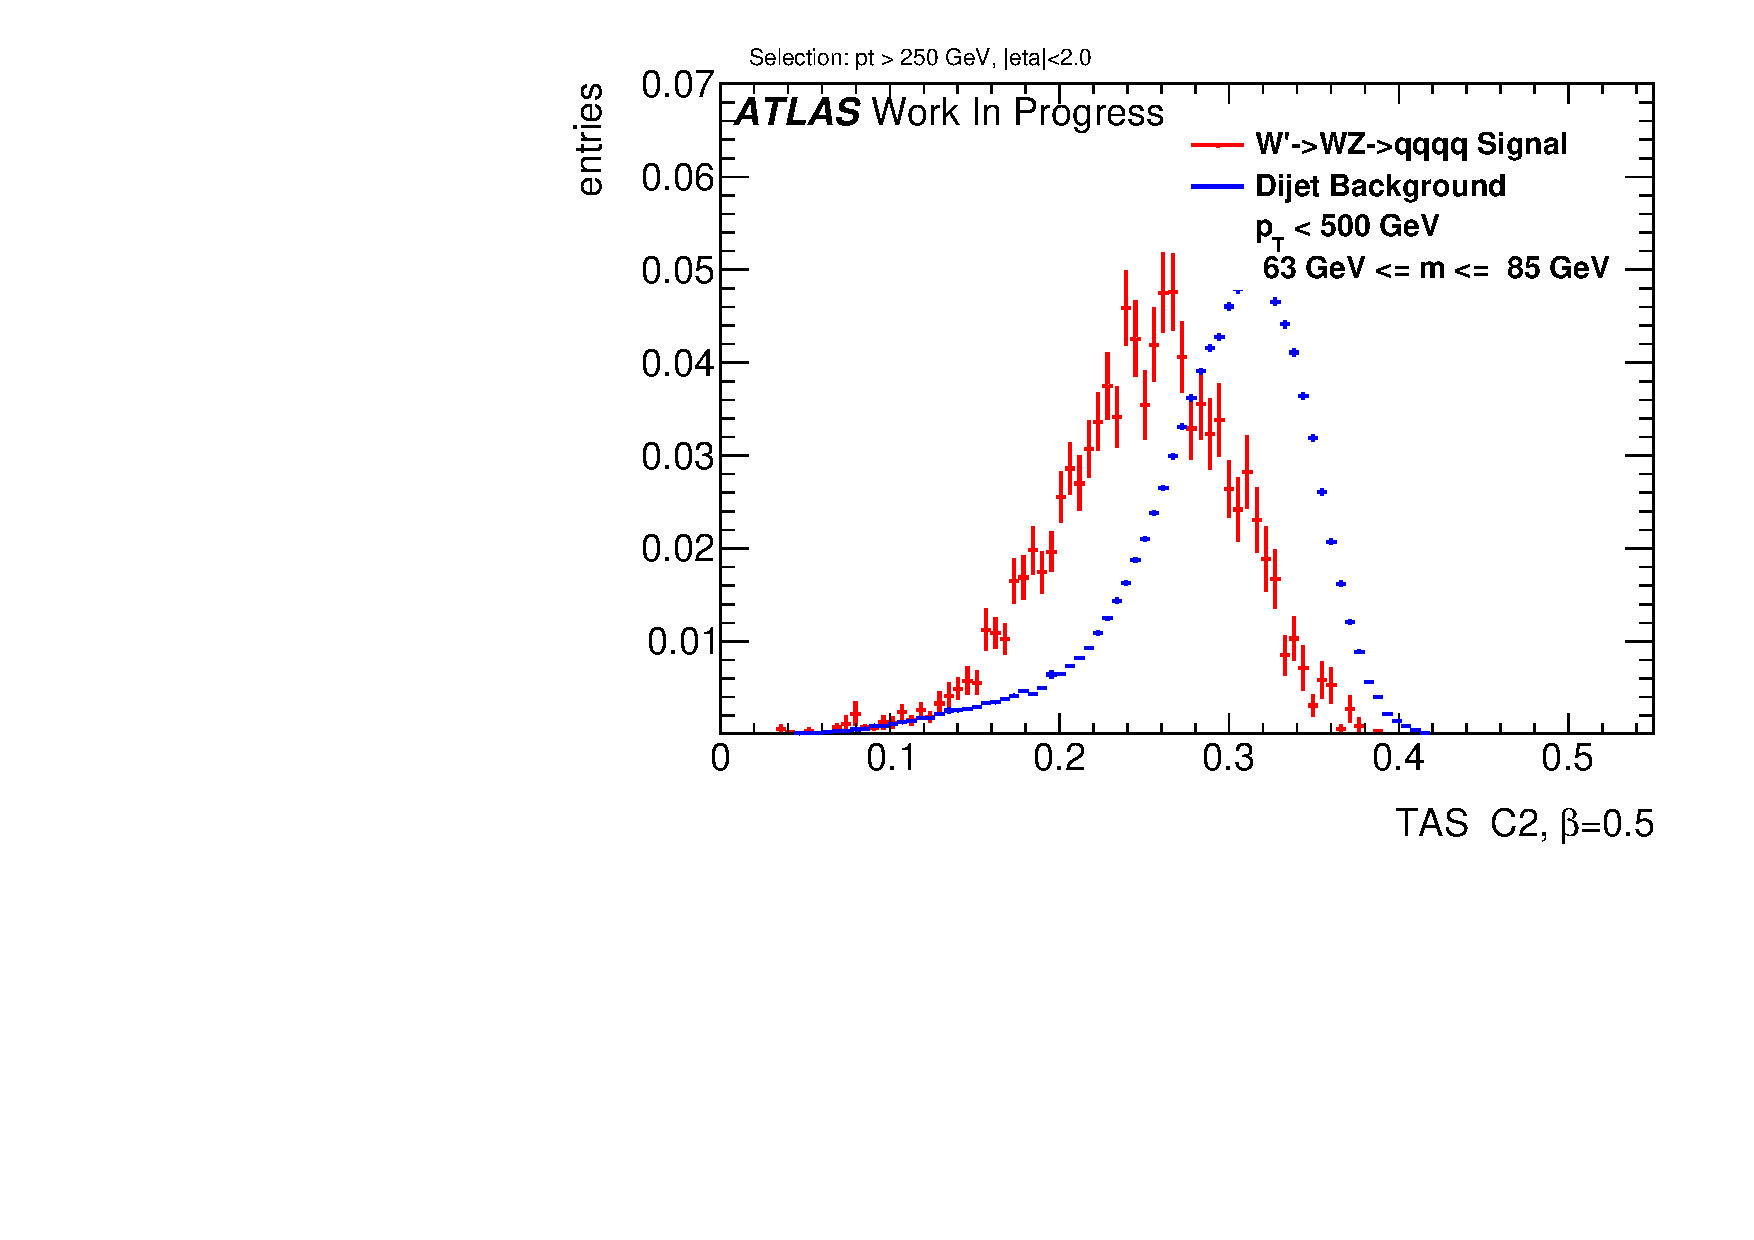
\includegraphics[width=0.3\textwidth]{sascha_input/Appendix/Distributions/w/distributions/beta05/h_assisted_tj_C2_05_bin1.pdf} \hspace{1mm}
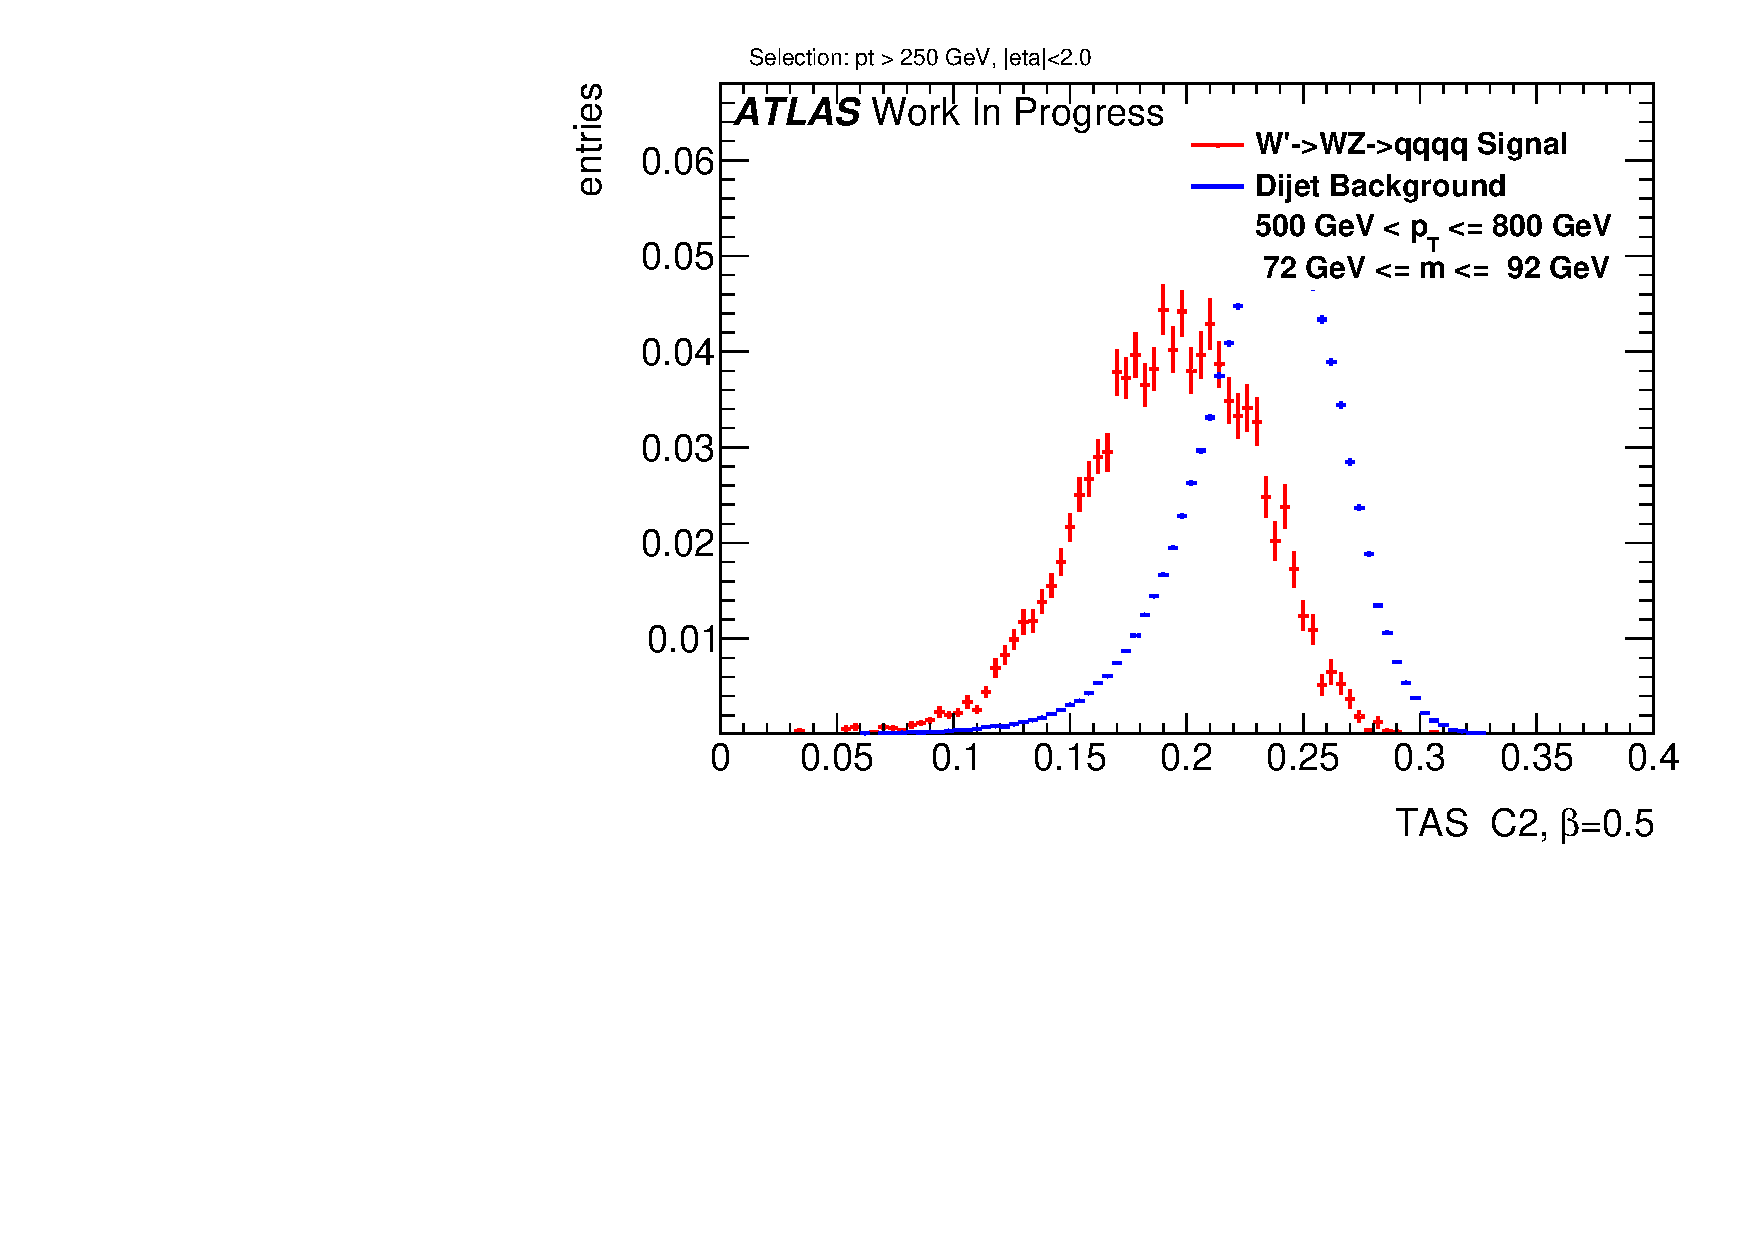
\includegraphics[width=0.3\textwidth]{sascha_input/Appendix/Distributions/w/distributions/beta05/h_assisted_tj_C2_05_bin2.pdf} \hspace{1mm}
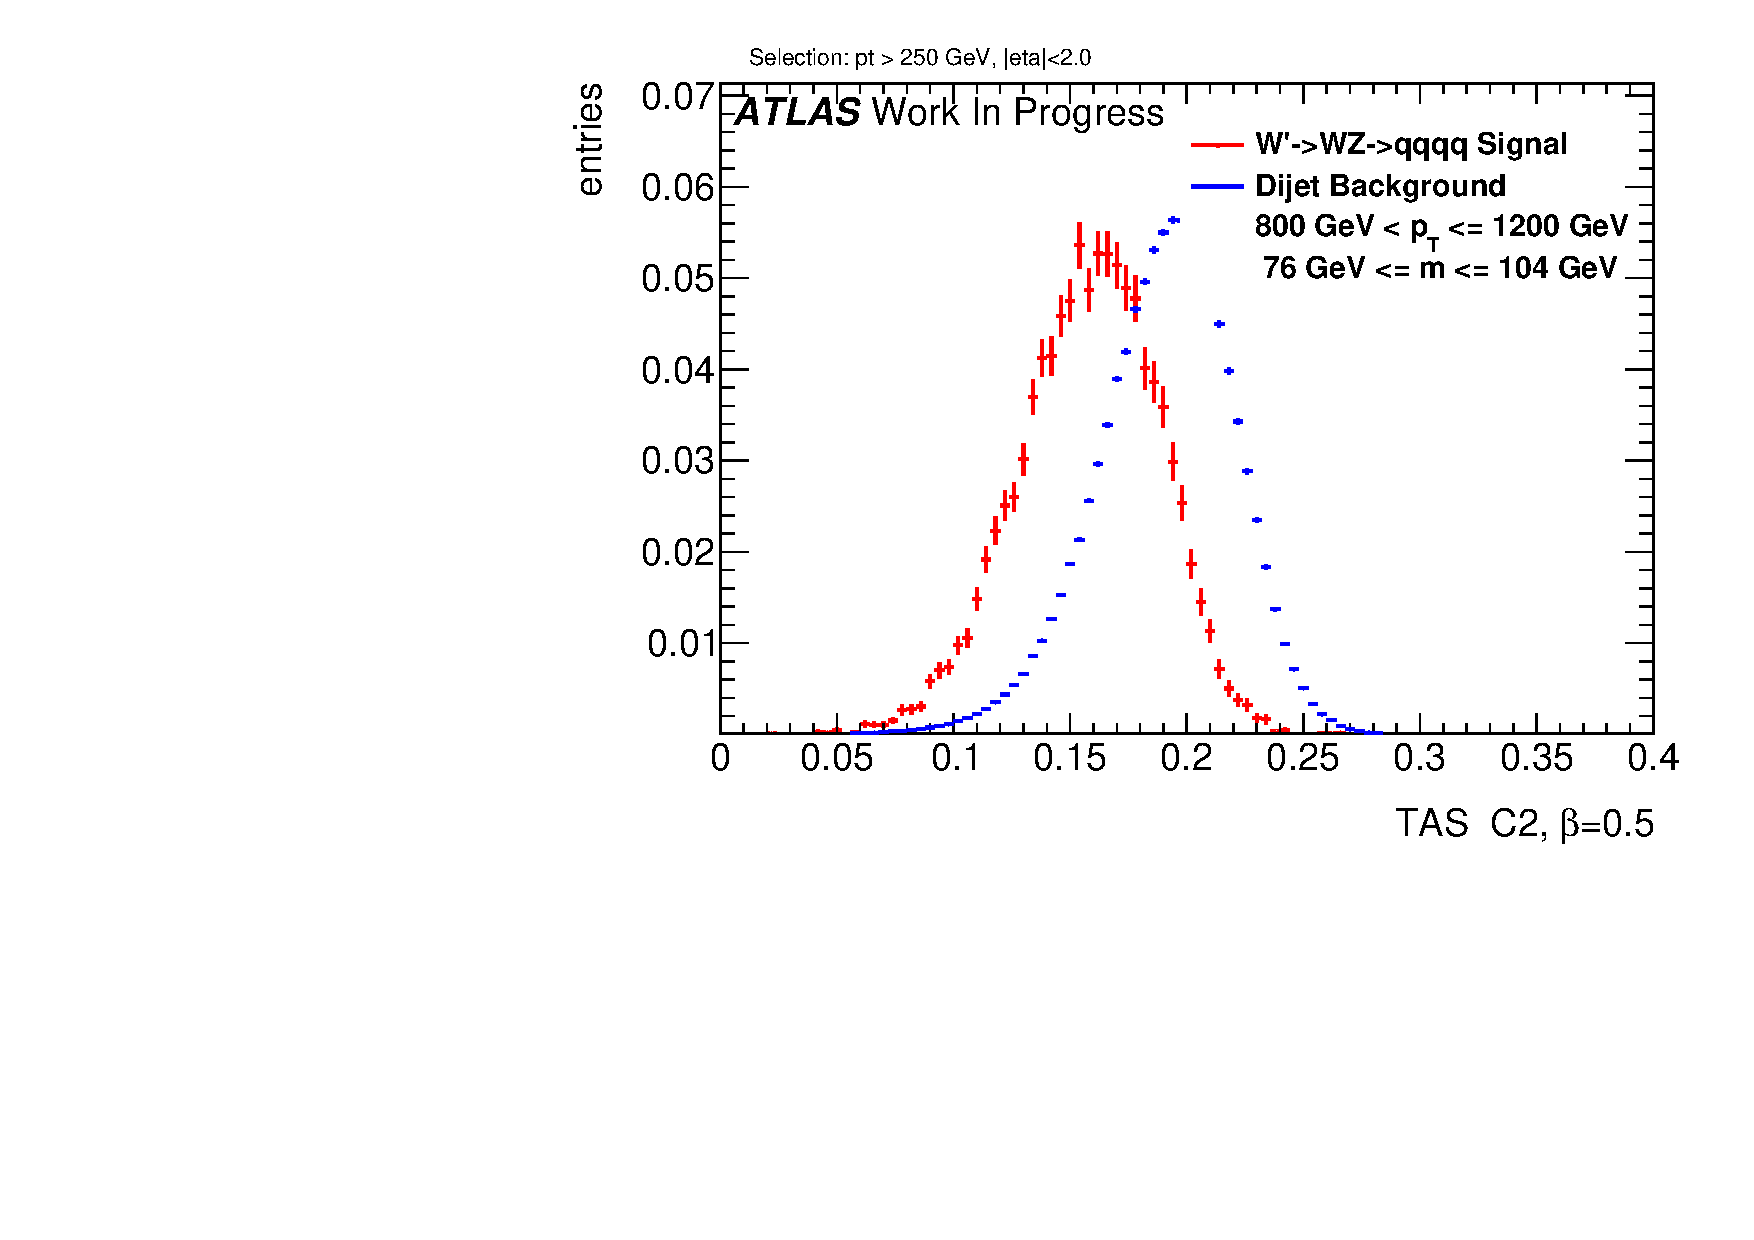
\includegraphics[width=0.3\textwidth]{sascha_input/Appendix/Distributions/w/distributions/beta05/h_assisted_tj_C2_05_bin3.pdf} 
\bigskip
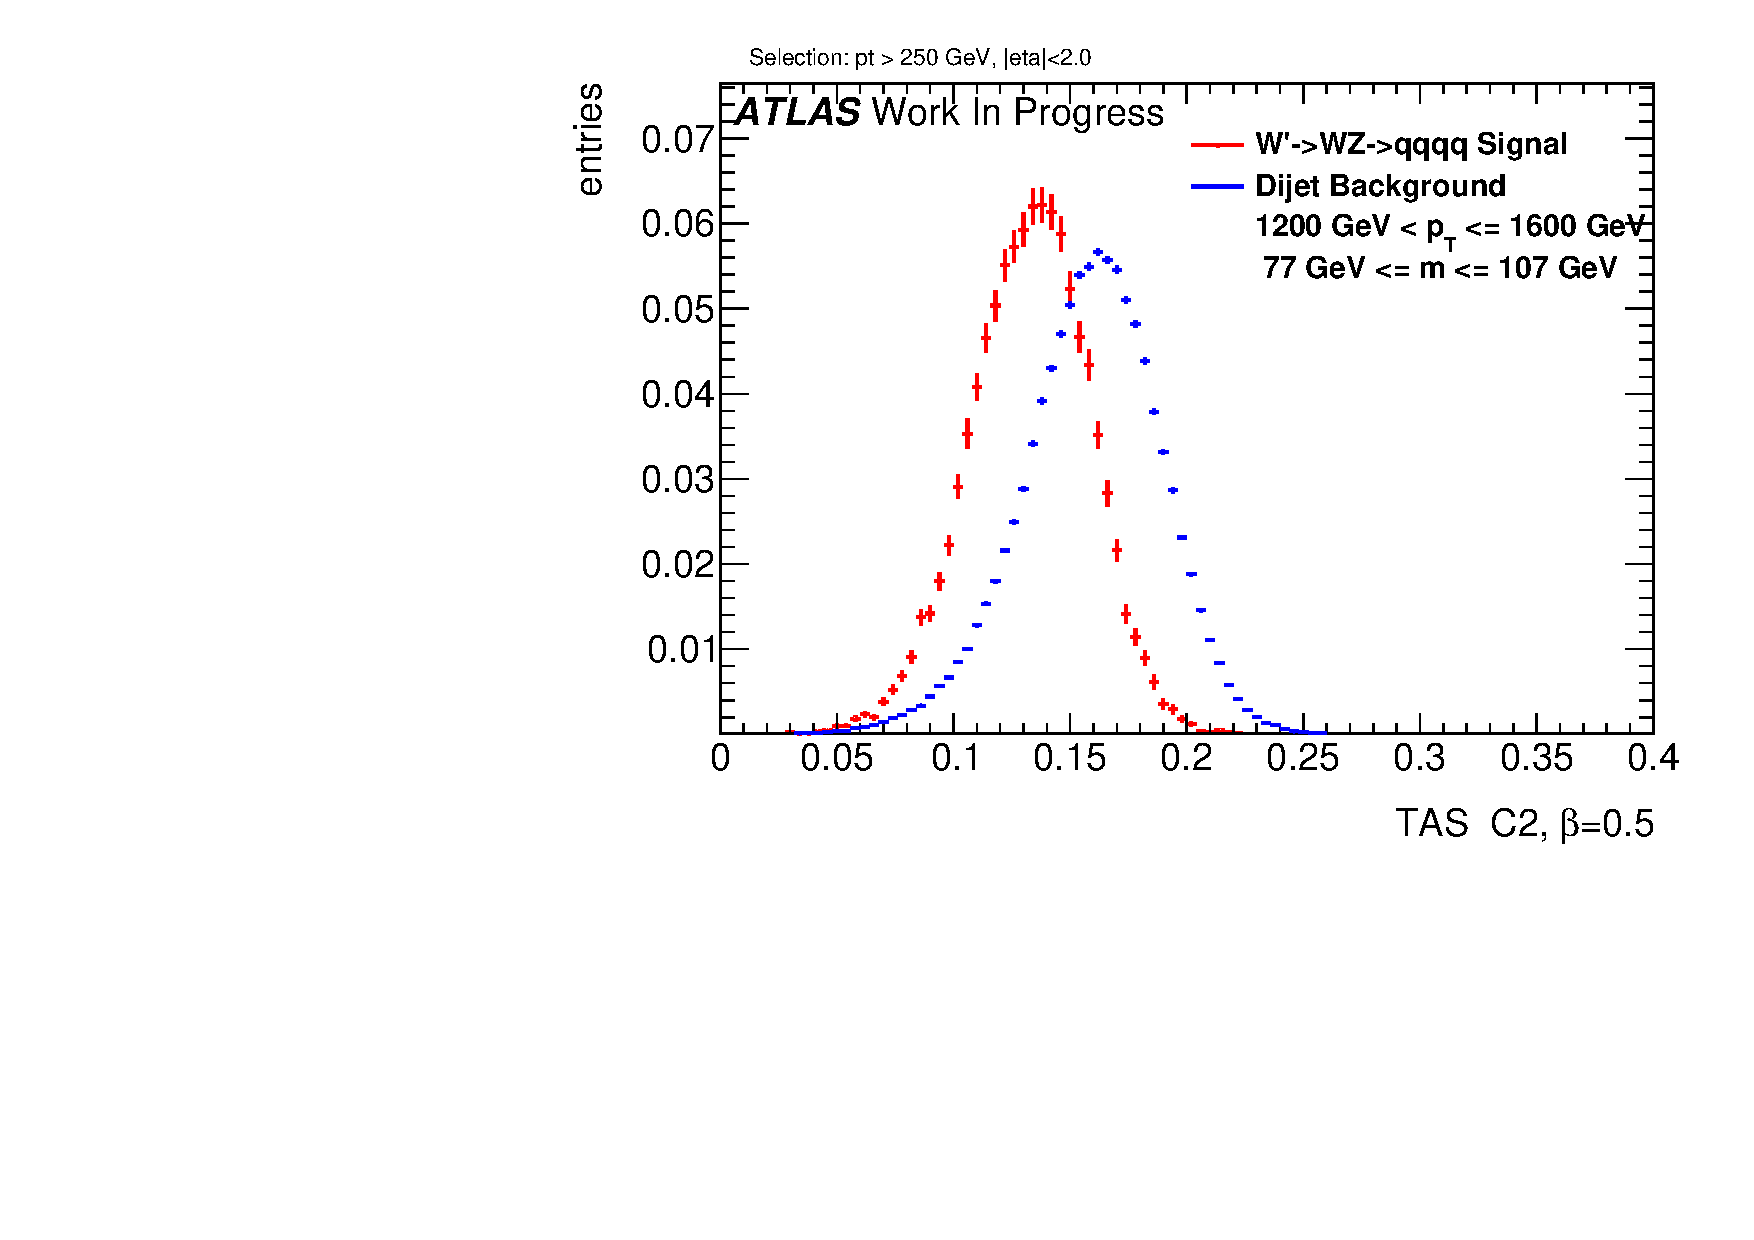
\includegraphics[width=0.3\textwidth]{sascha_input/Appendix/Distributions/w/distributions/beta05/h_assisted_tj_C2_05_bin4.pdf} \hspace{1mm}
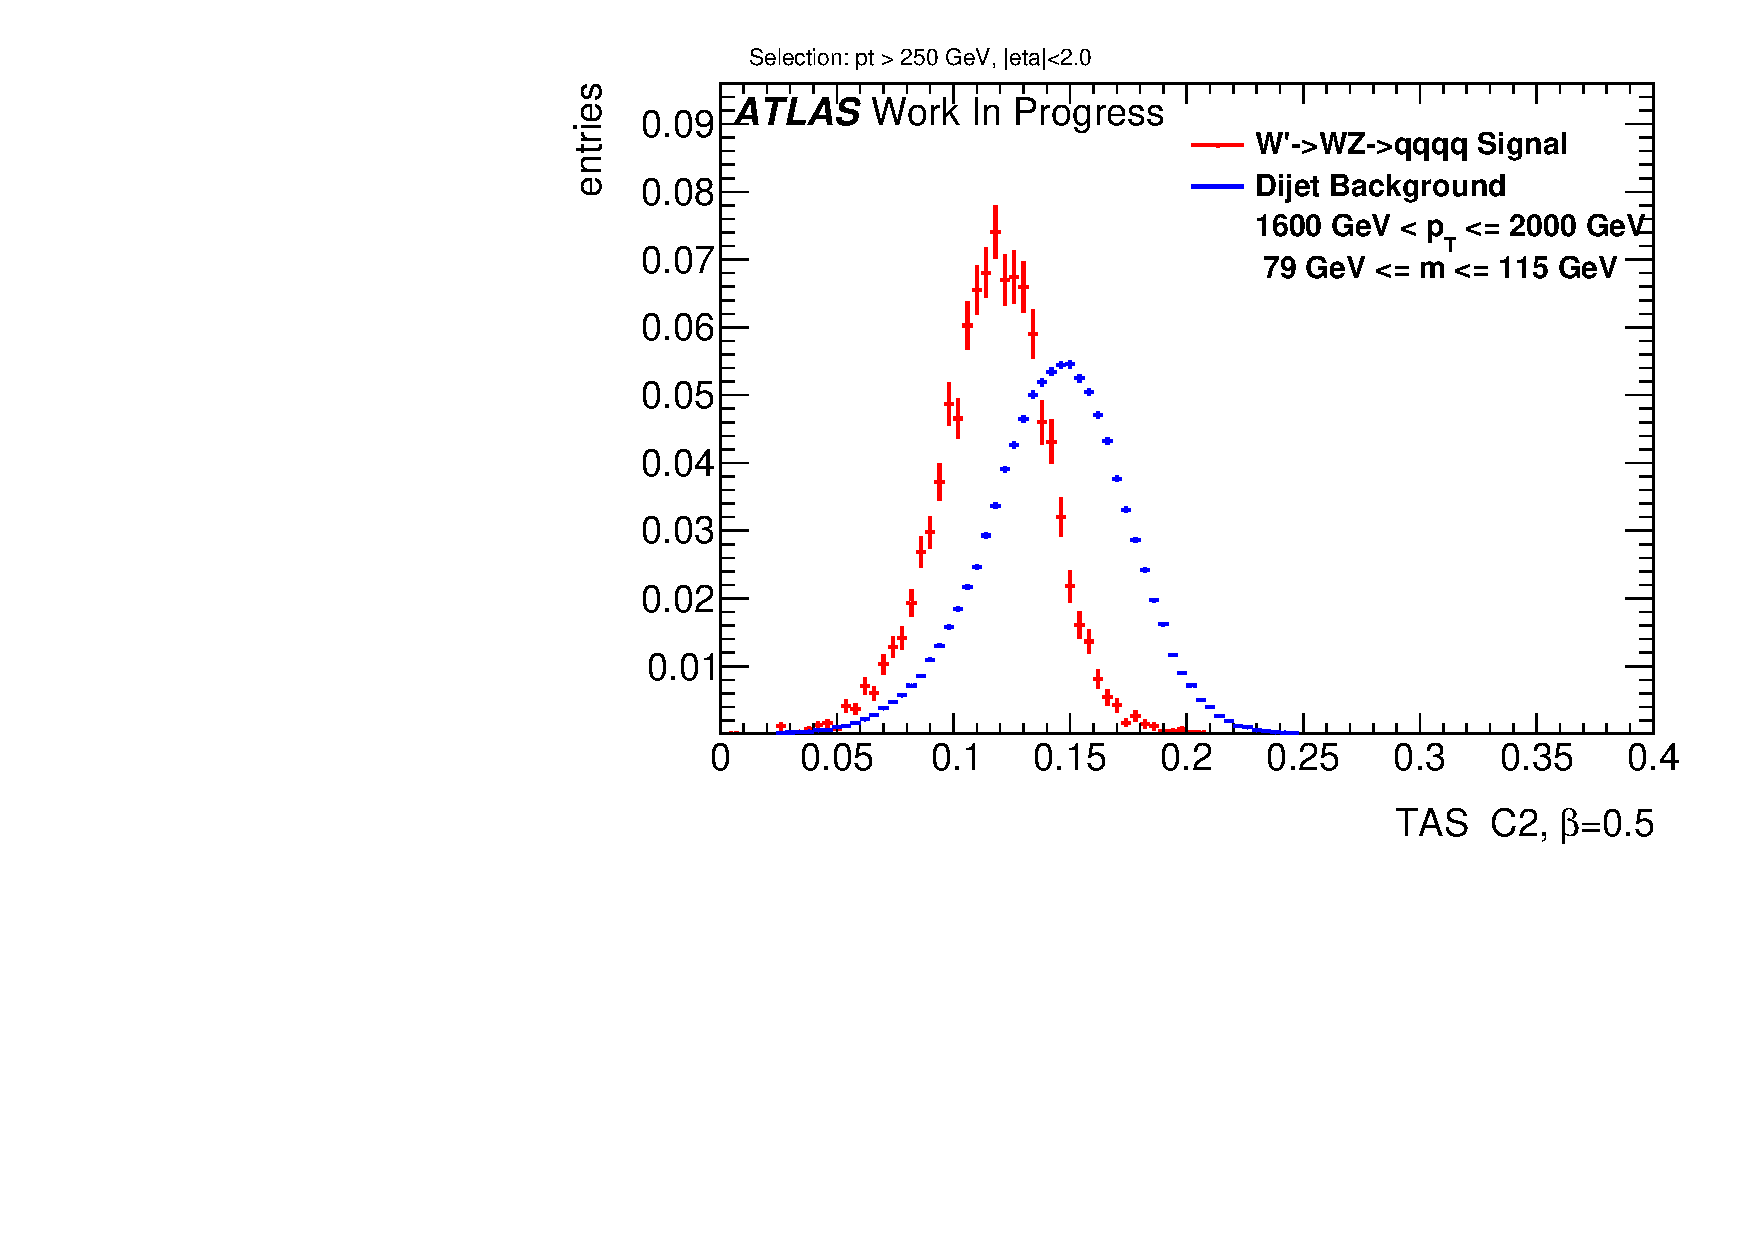
\includegraphics[width=0.3\textwidth]{sascha_input/Appendix/Distributions/w/distributions/beta05/h_assisted_tj_C2_05_bin5.pdf} \hspace{1mm}
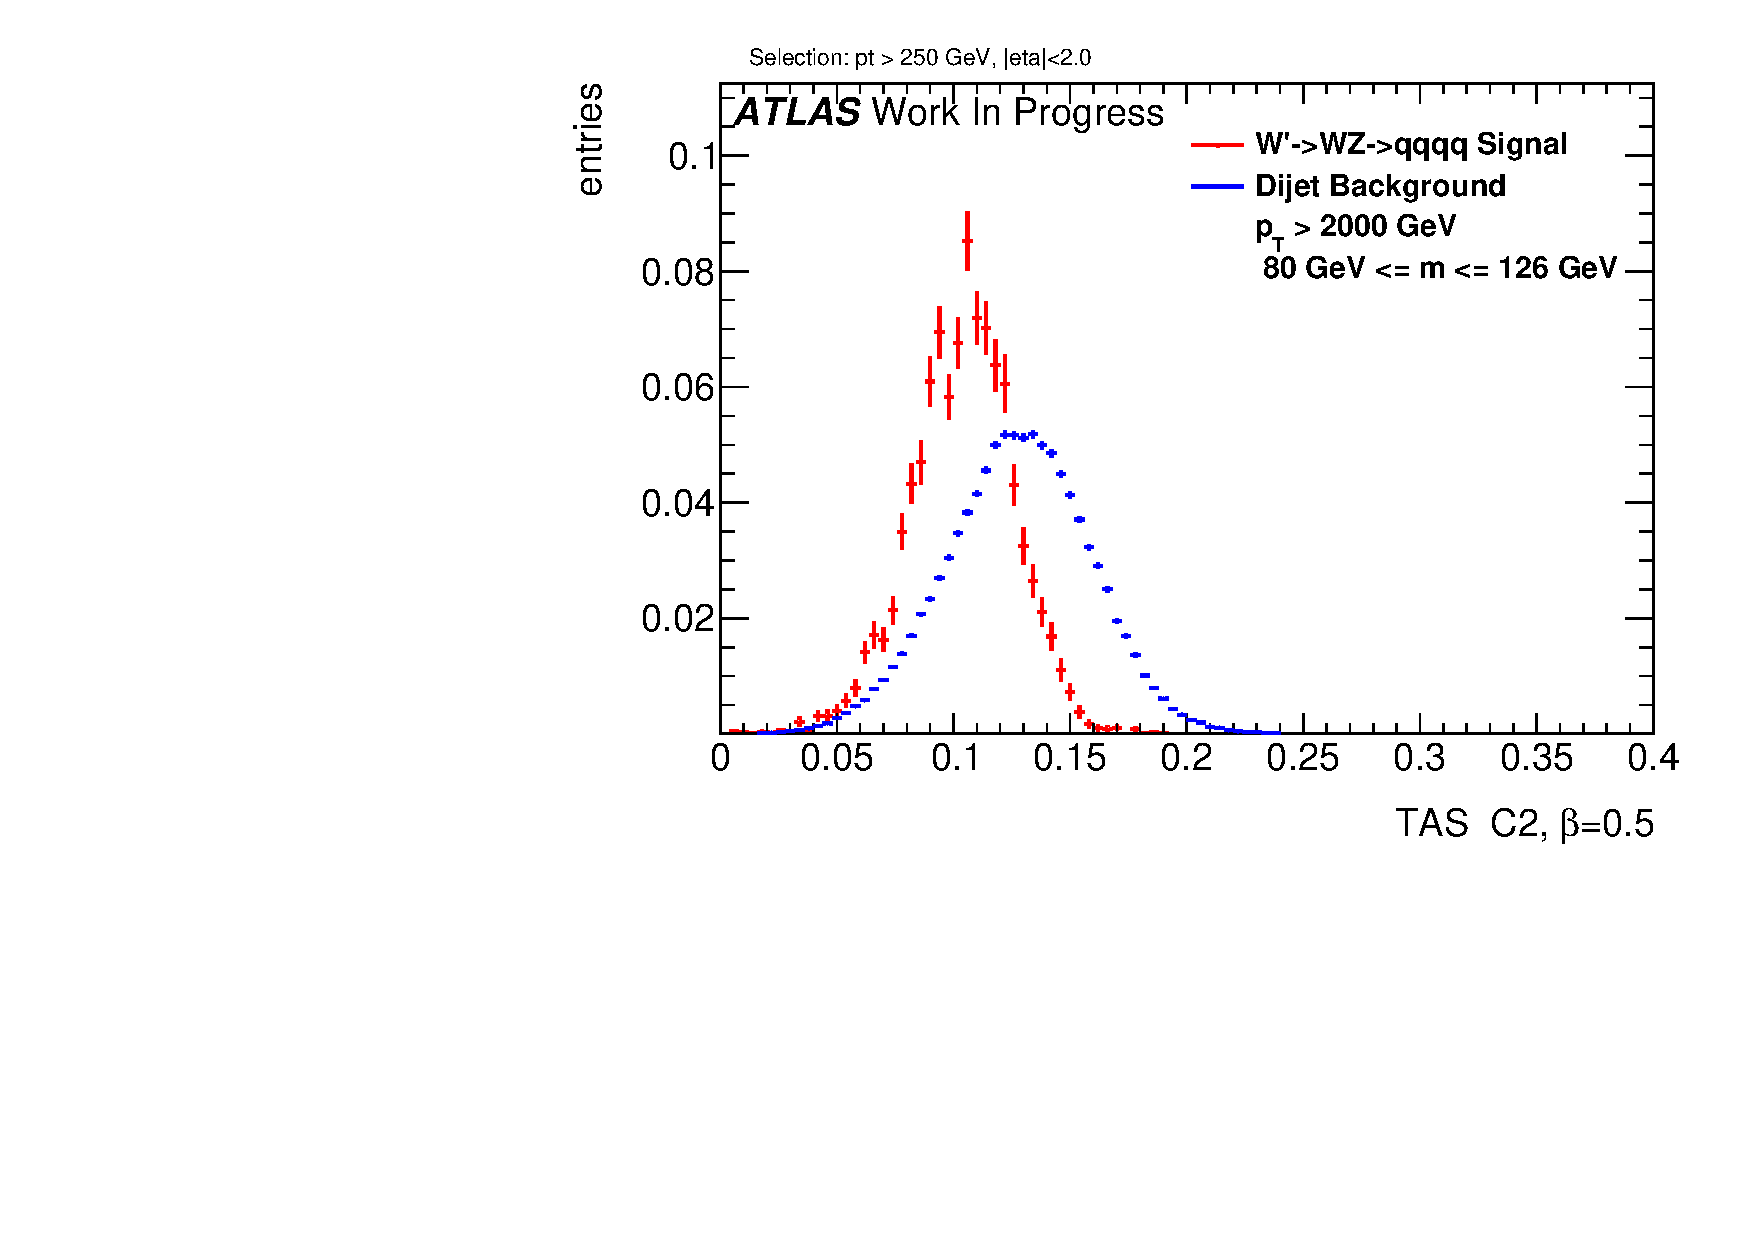
\includegraphics[width=0.3\textwidth]{sascha_input/Appendix/Distributions/w/distributions/beta05/h_assisted_tj_C2_05_bin6.pdf} 
\bigskip
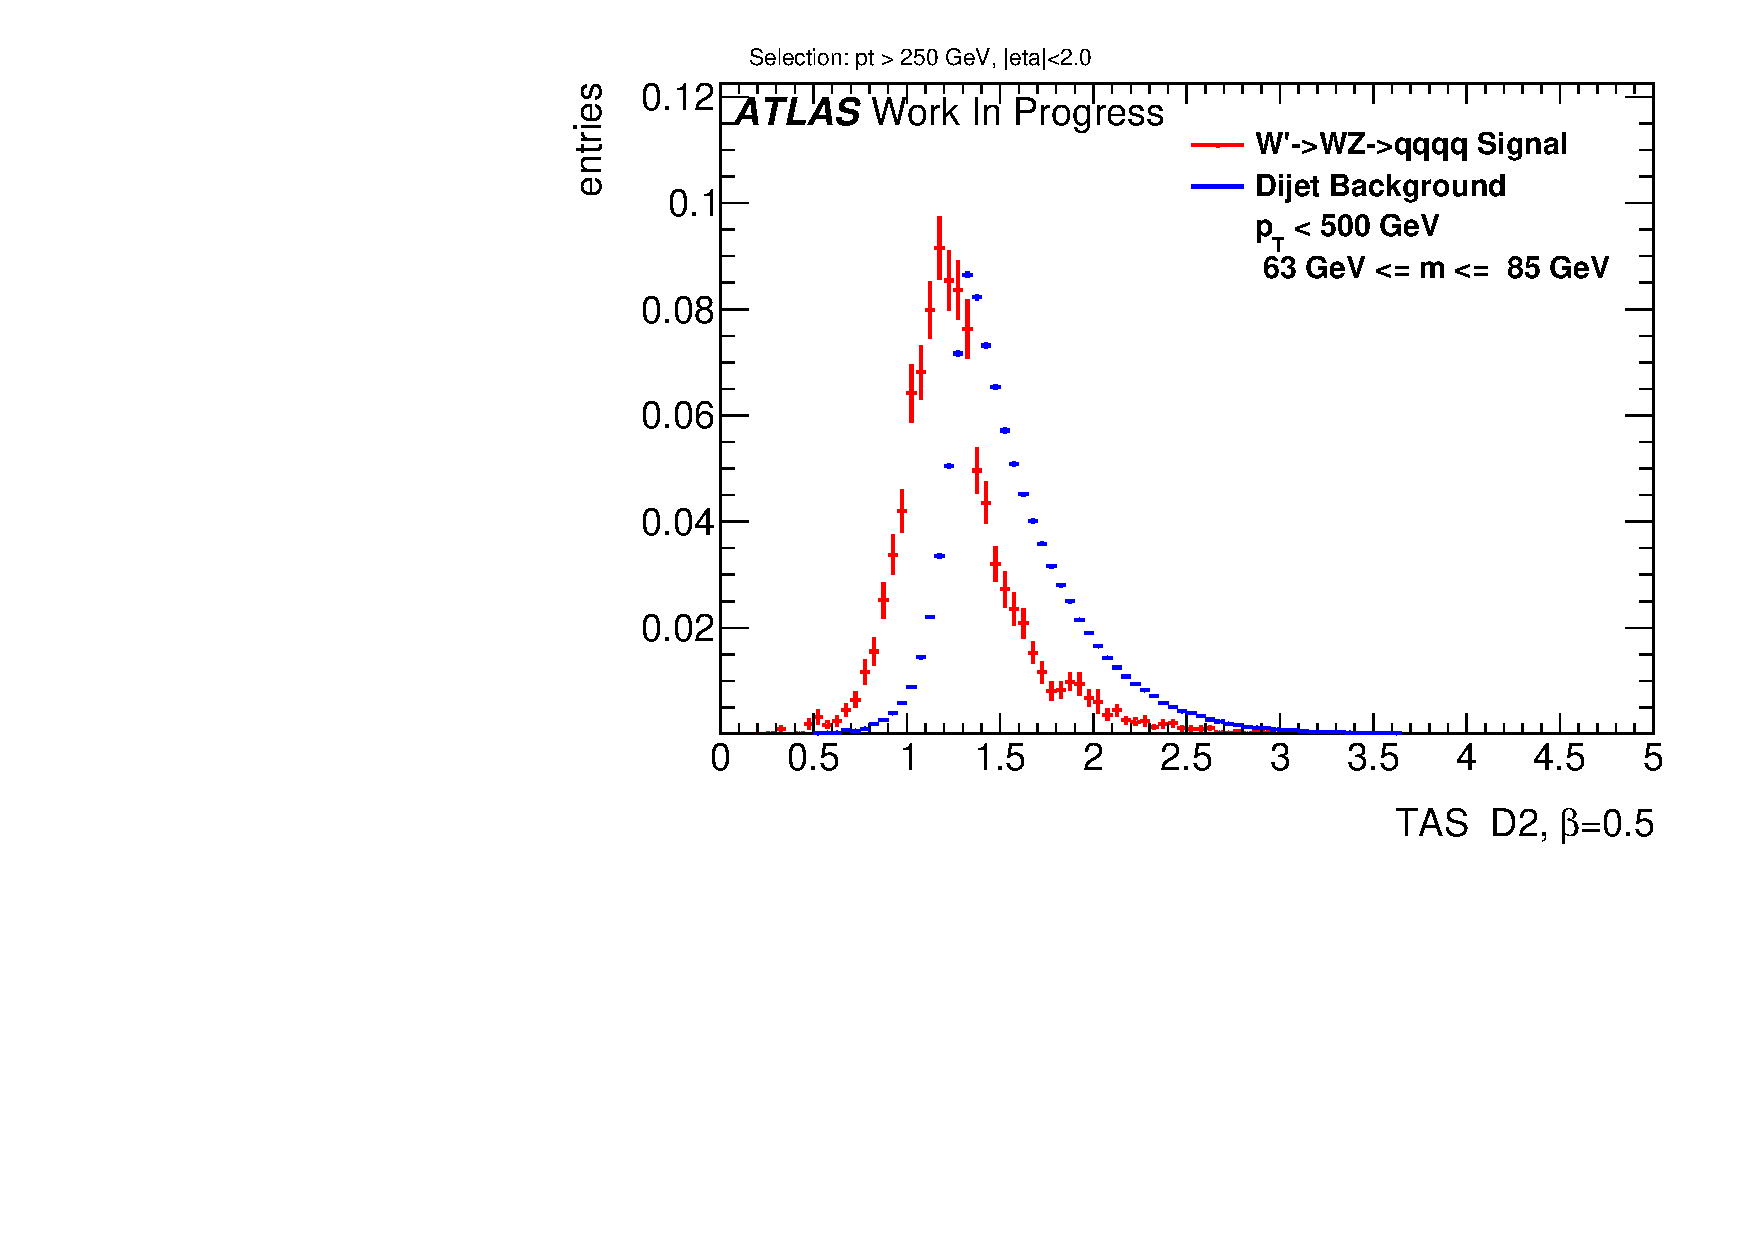
\includegraphics[width=0.3\textwidth]{sascha_input/Appendix/Distributions/w/distributions/beta05/h_assisted_tj_D2_05_bin1.pdf} \hspace{1mm}
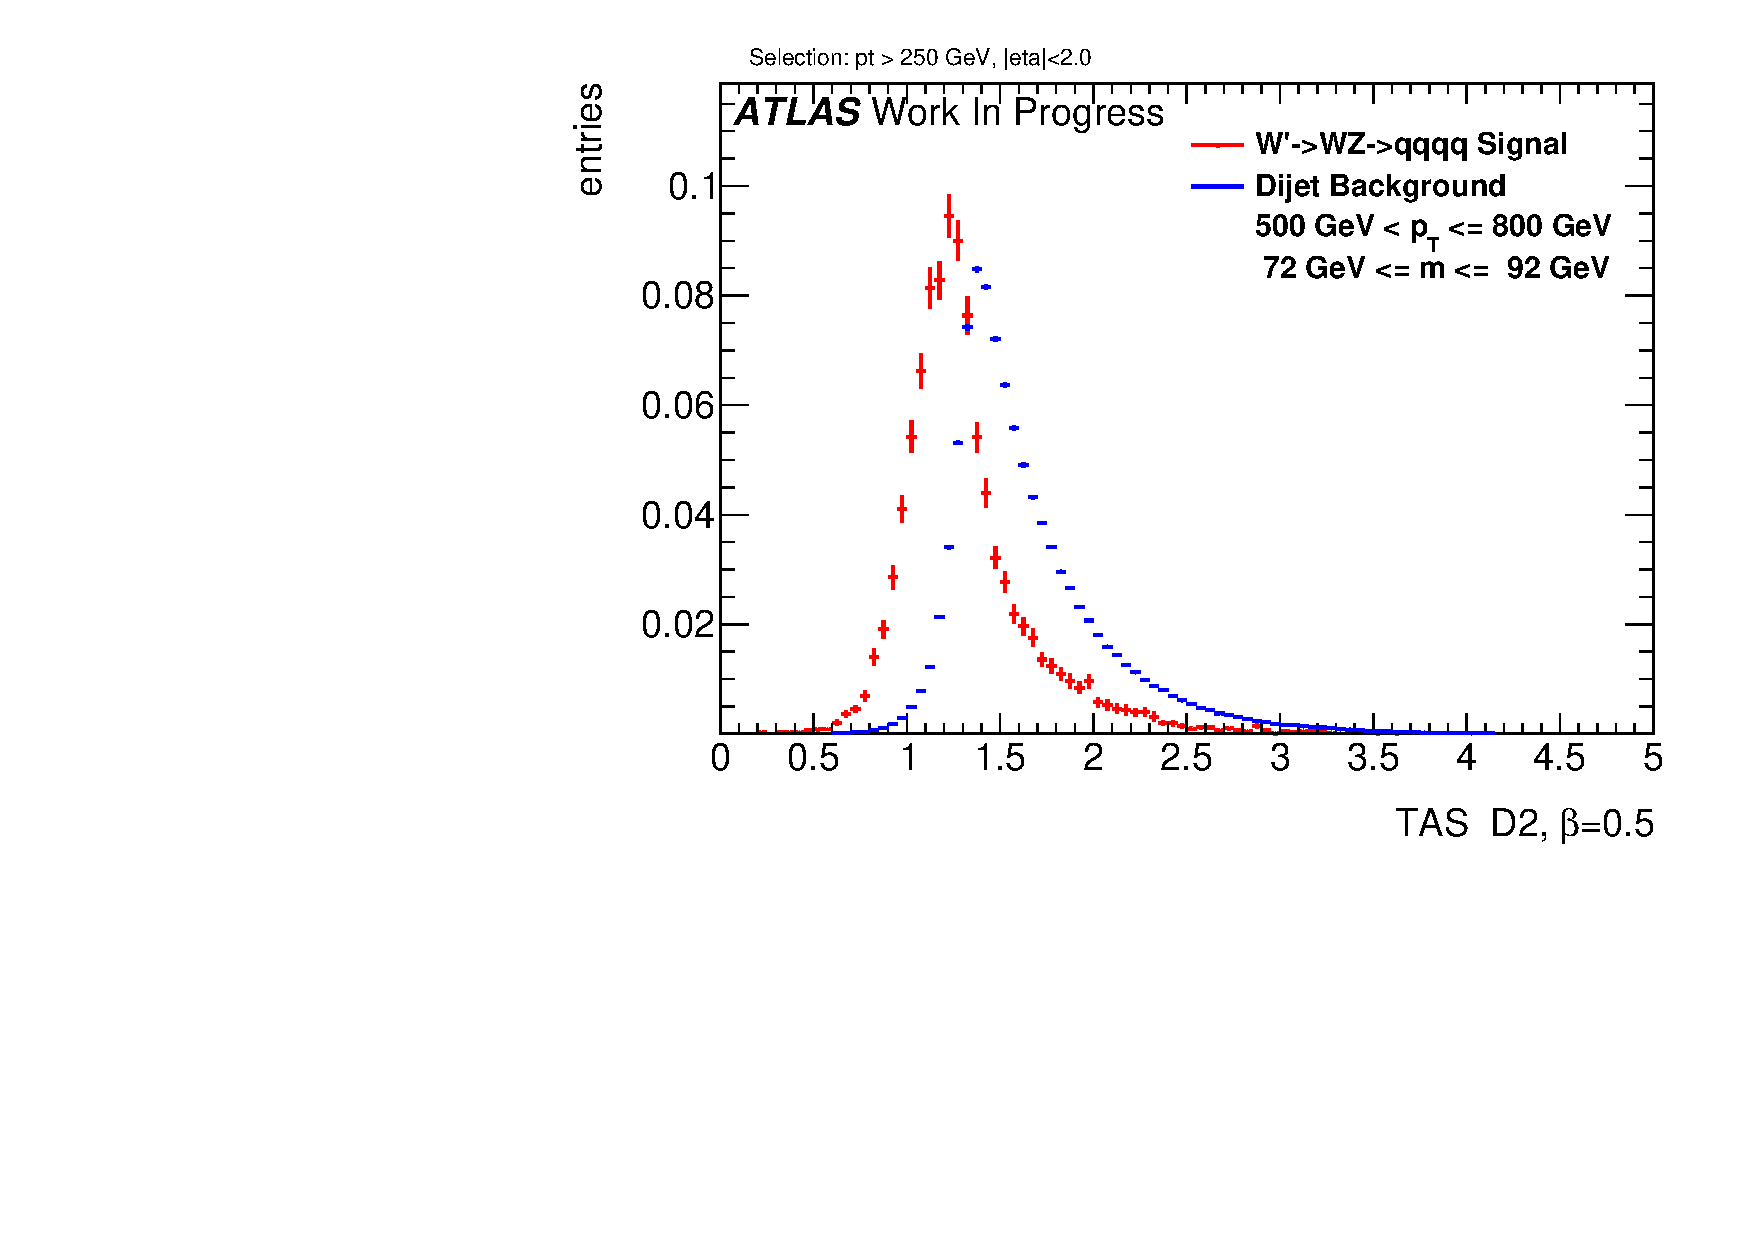
\includegraphics[width=0.3\textwidth]{sascha_input/Appendix/Distributions/w/distributions/beta05/h_assisted_tj_D2_05_bin2.pdf} \hspace{1mm}
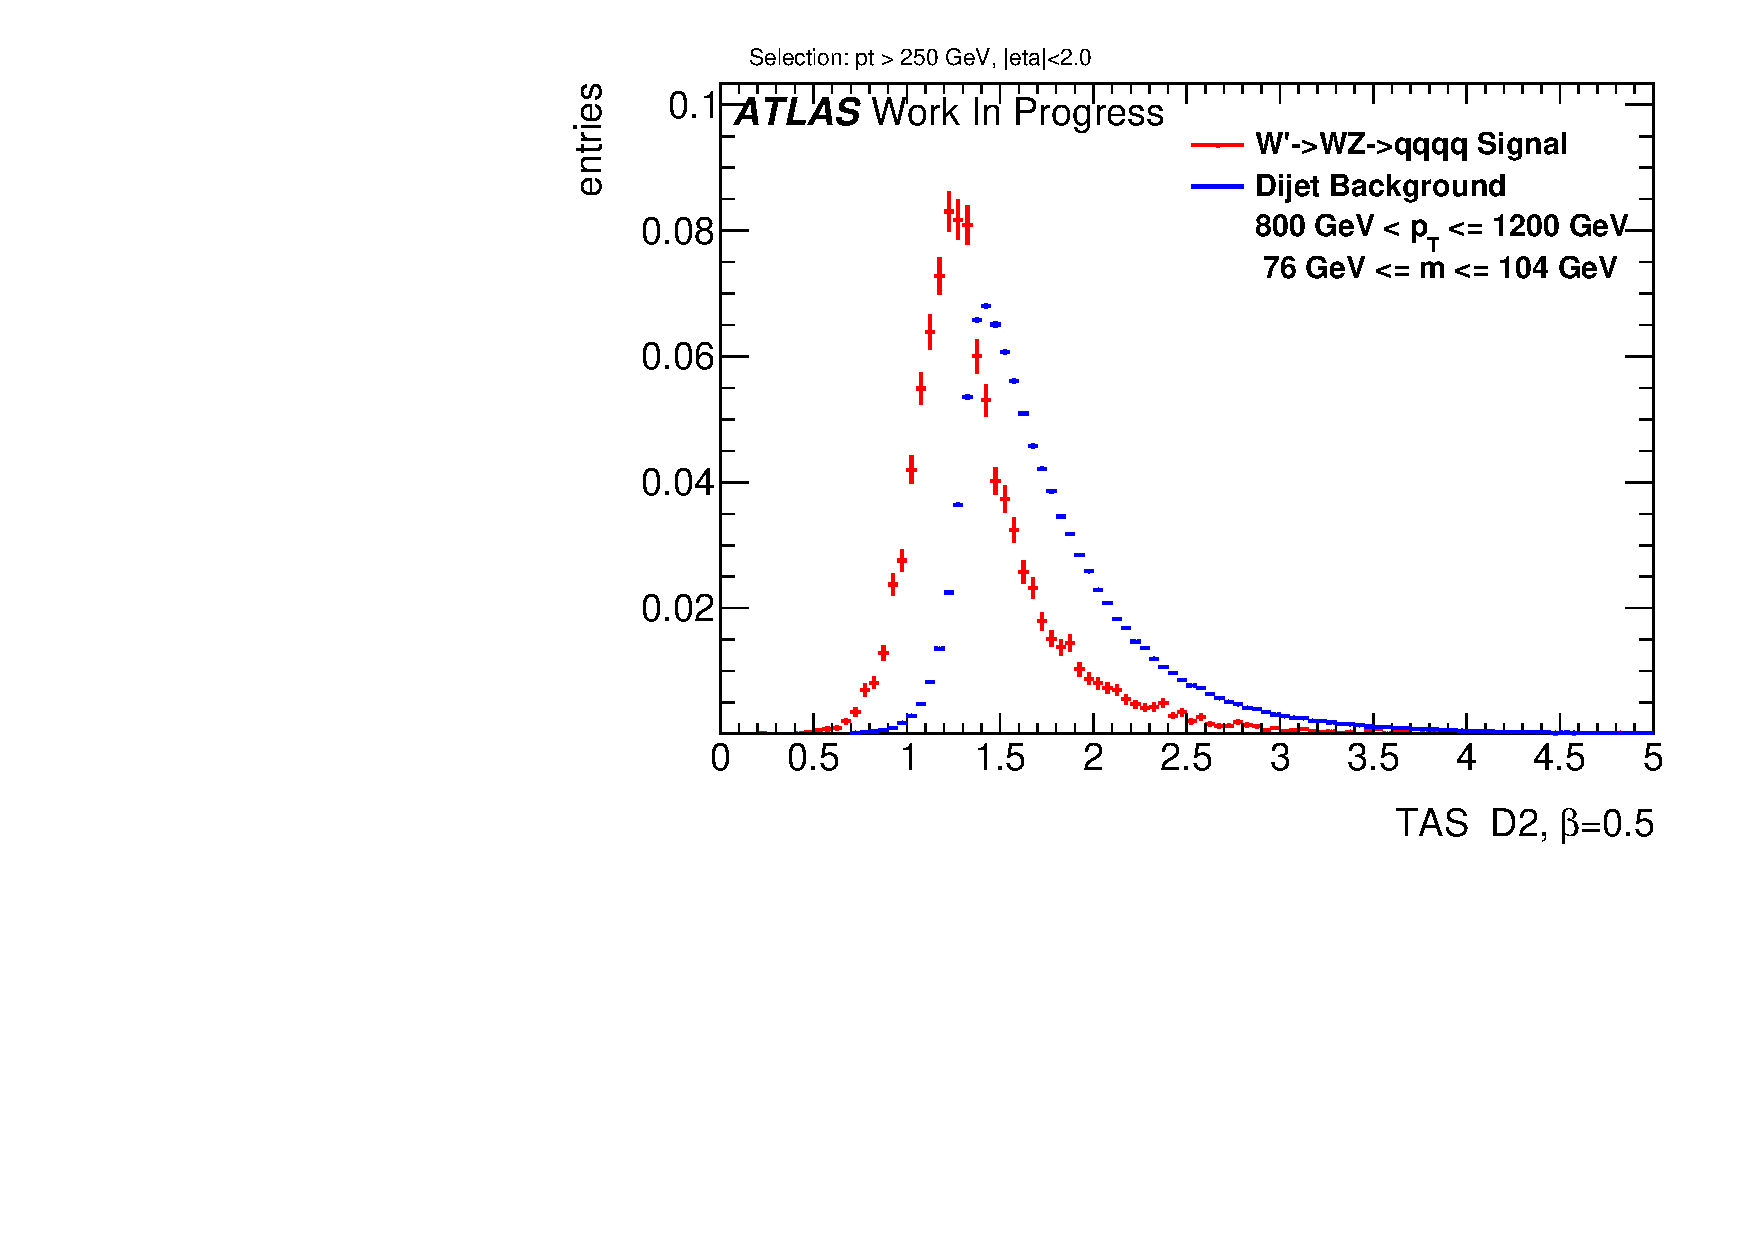
\includegraphics[width=0.3\textwidth]{sascha_input/Appendix/Distributions/w/distributions/beta05/h_assisted_tj_D2_05_bin3.pdf} 
\bigskip
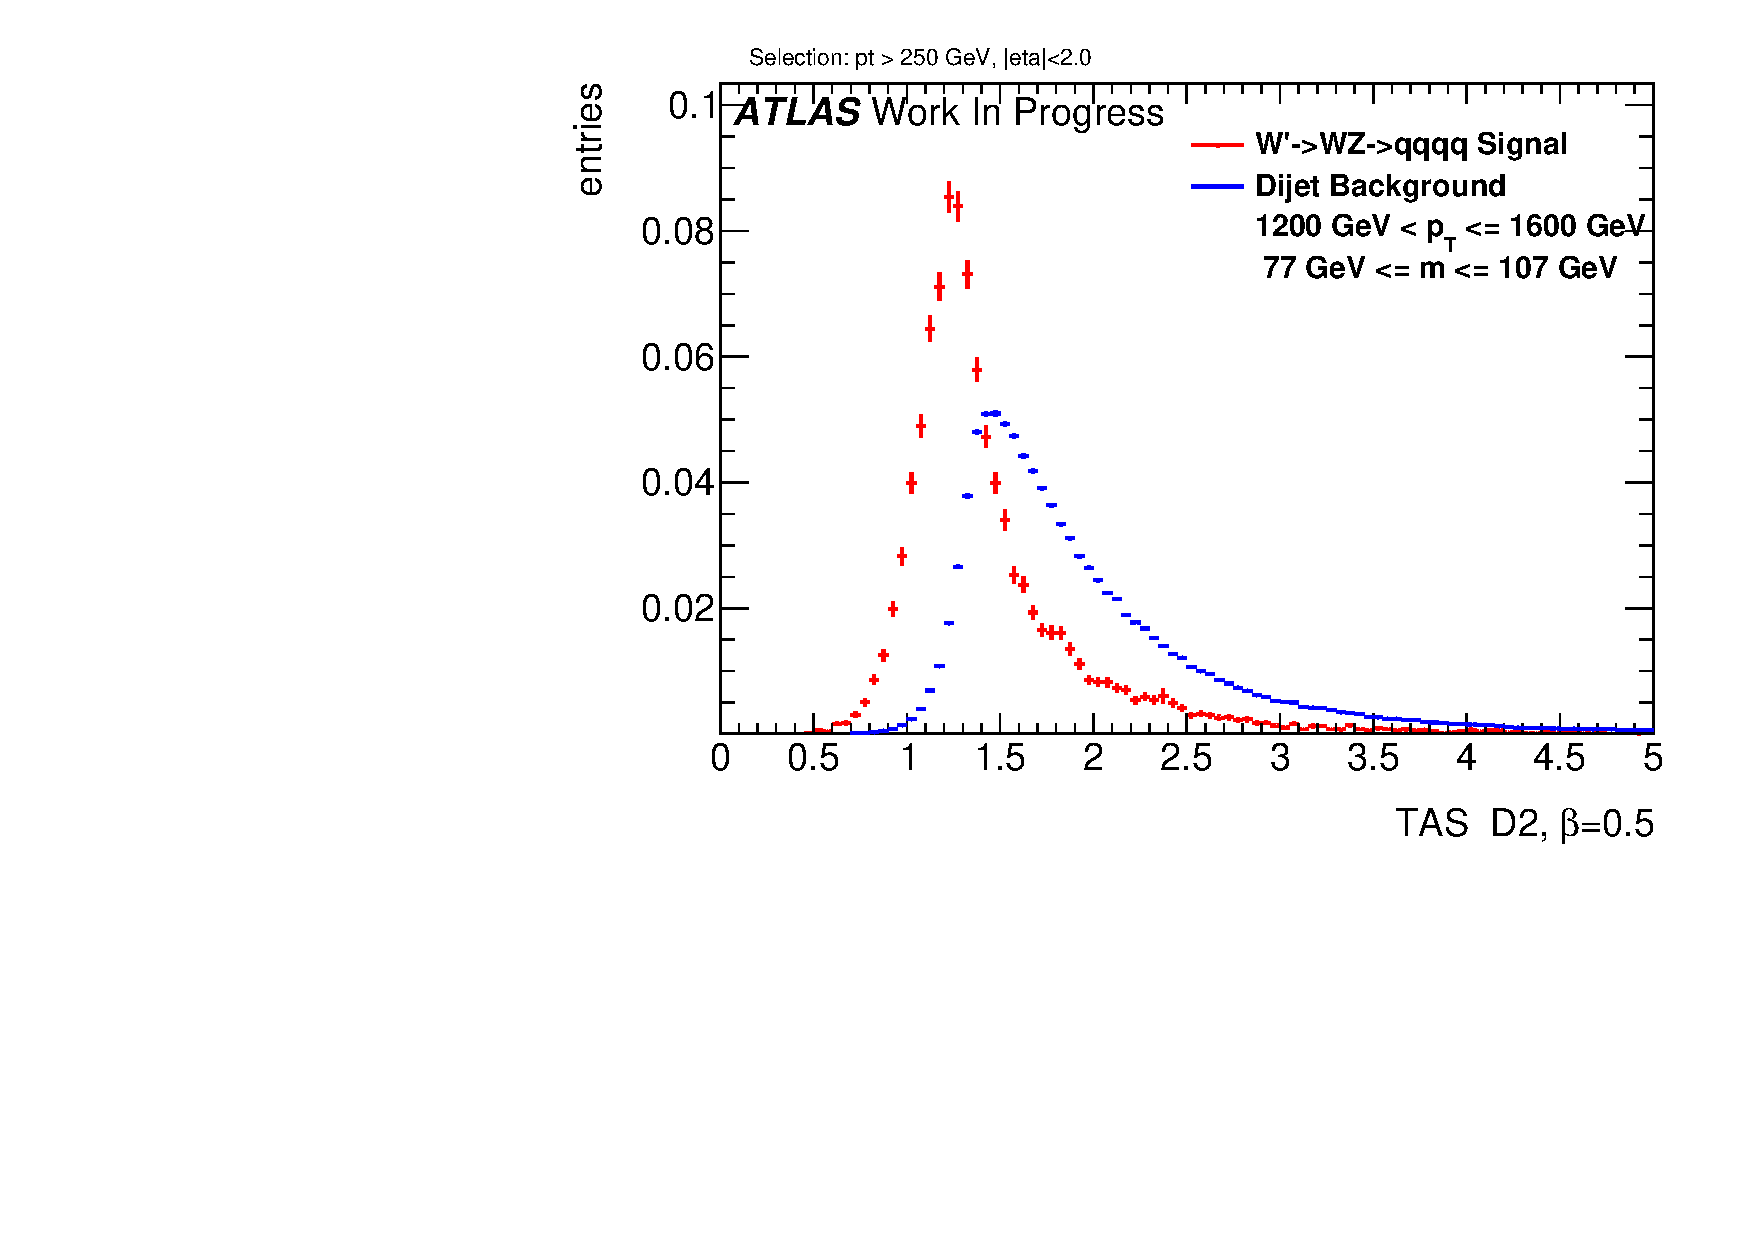
\includegraphics[width=0.3\textwidth]{sascha_input/Appendix/Distributions/w/distributions/beta05/h_assisted_tj_D2_05_bin4.pdf} \hspace{1mm}
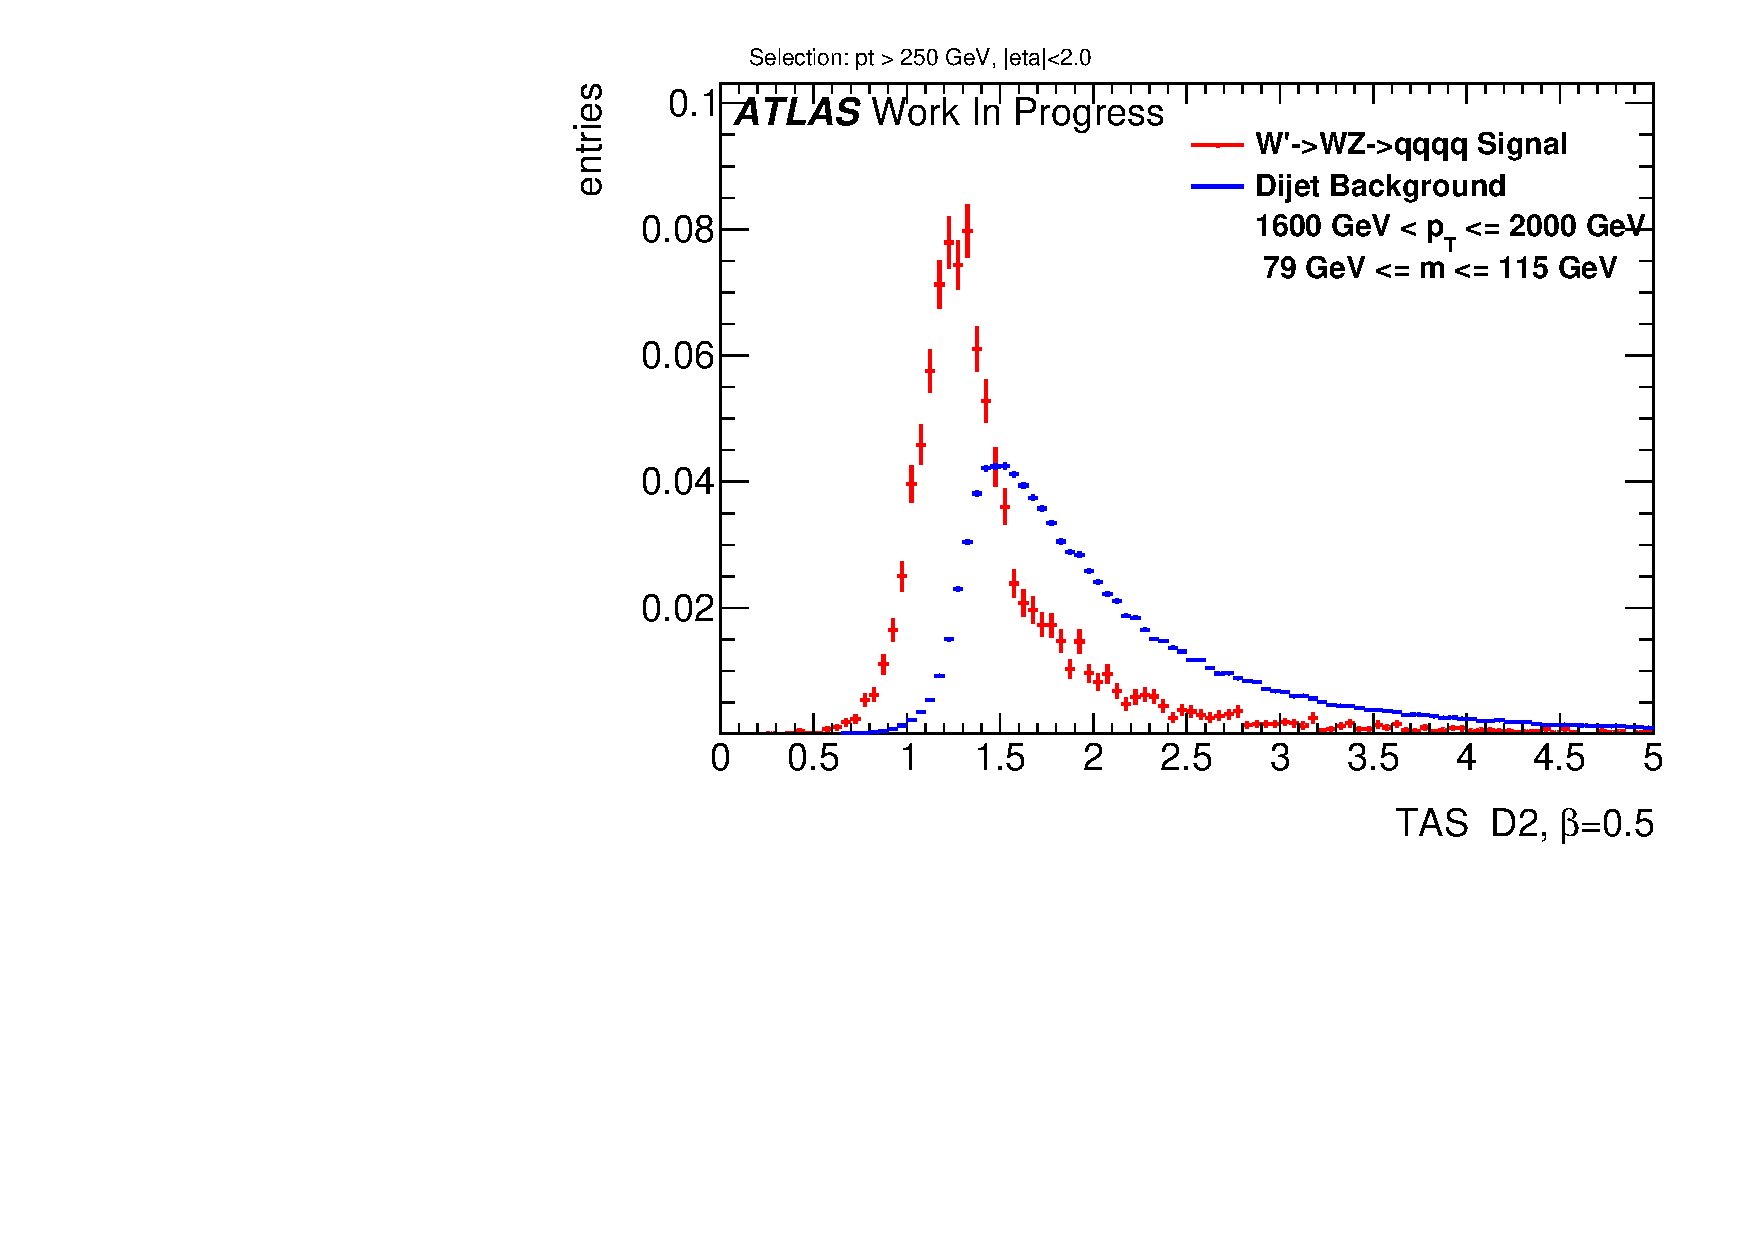
\includegraphics[width=0.3\textwidth]{sascha_input/Appendix/Distributions/w/distributions/beta05/h_assisted_tj_D2_05_bin5.pdf} \hspace{1mm}
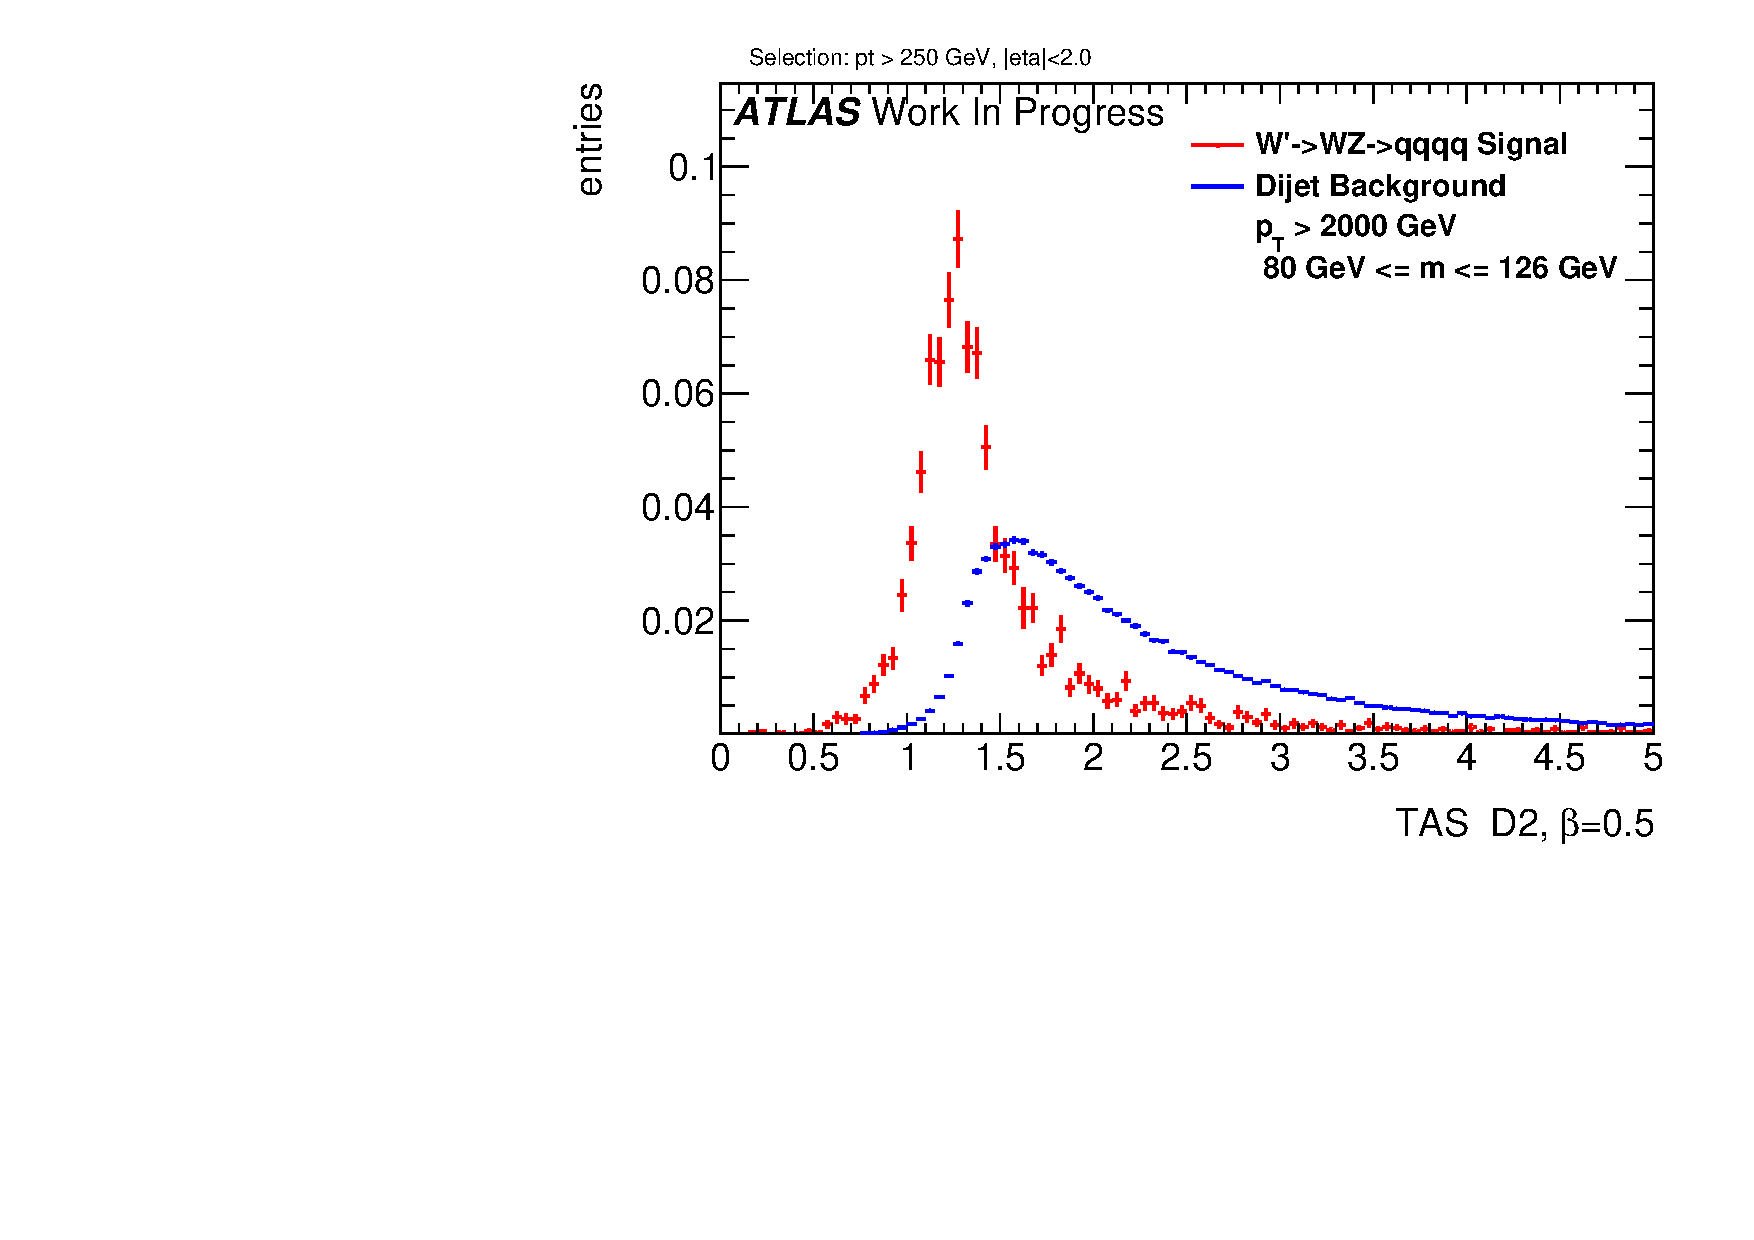
\includegraphics[width=0.3\textwidth]{sascha_input/Appendix/Distributions/w/distributions/beta05/h_assisted_tj_D2_05_bin6.pdf}
\bigskip 
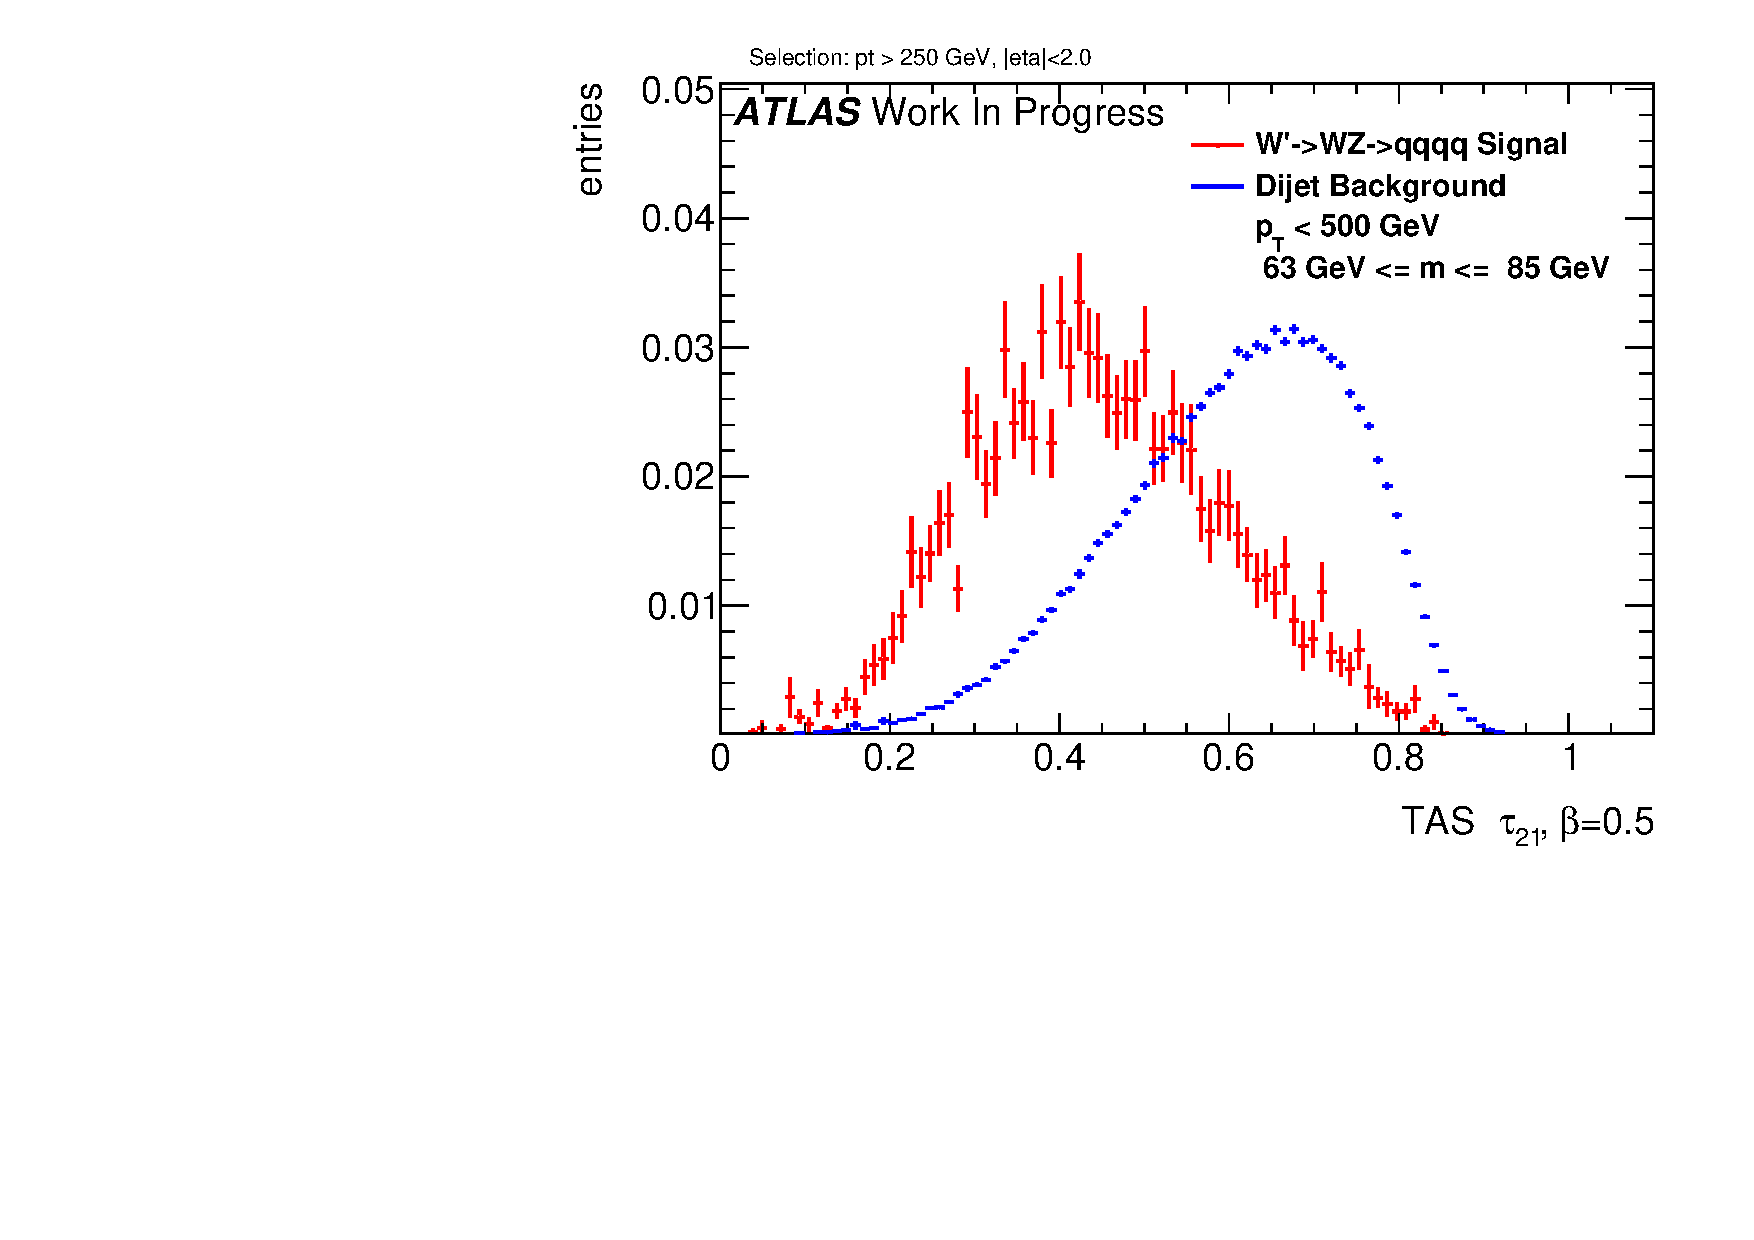
\includegraphics[width=0.3\textwidth]{sascha_input/Appendix/Distributions/w/distributions/beta05/h_assisted_tj_nSub21_05_bin1.pdf} \hspace{1mm}
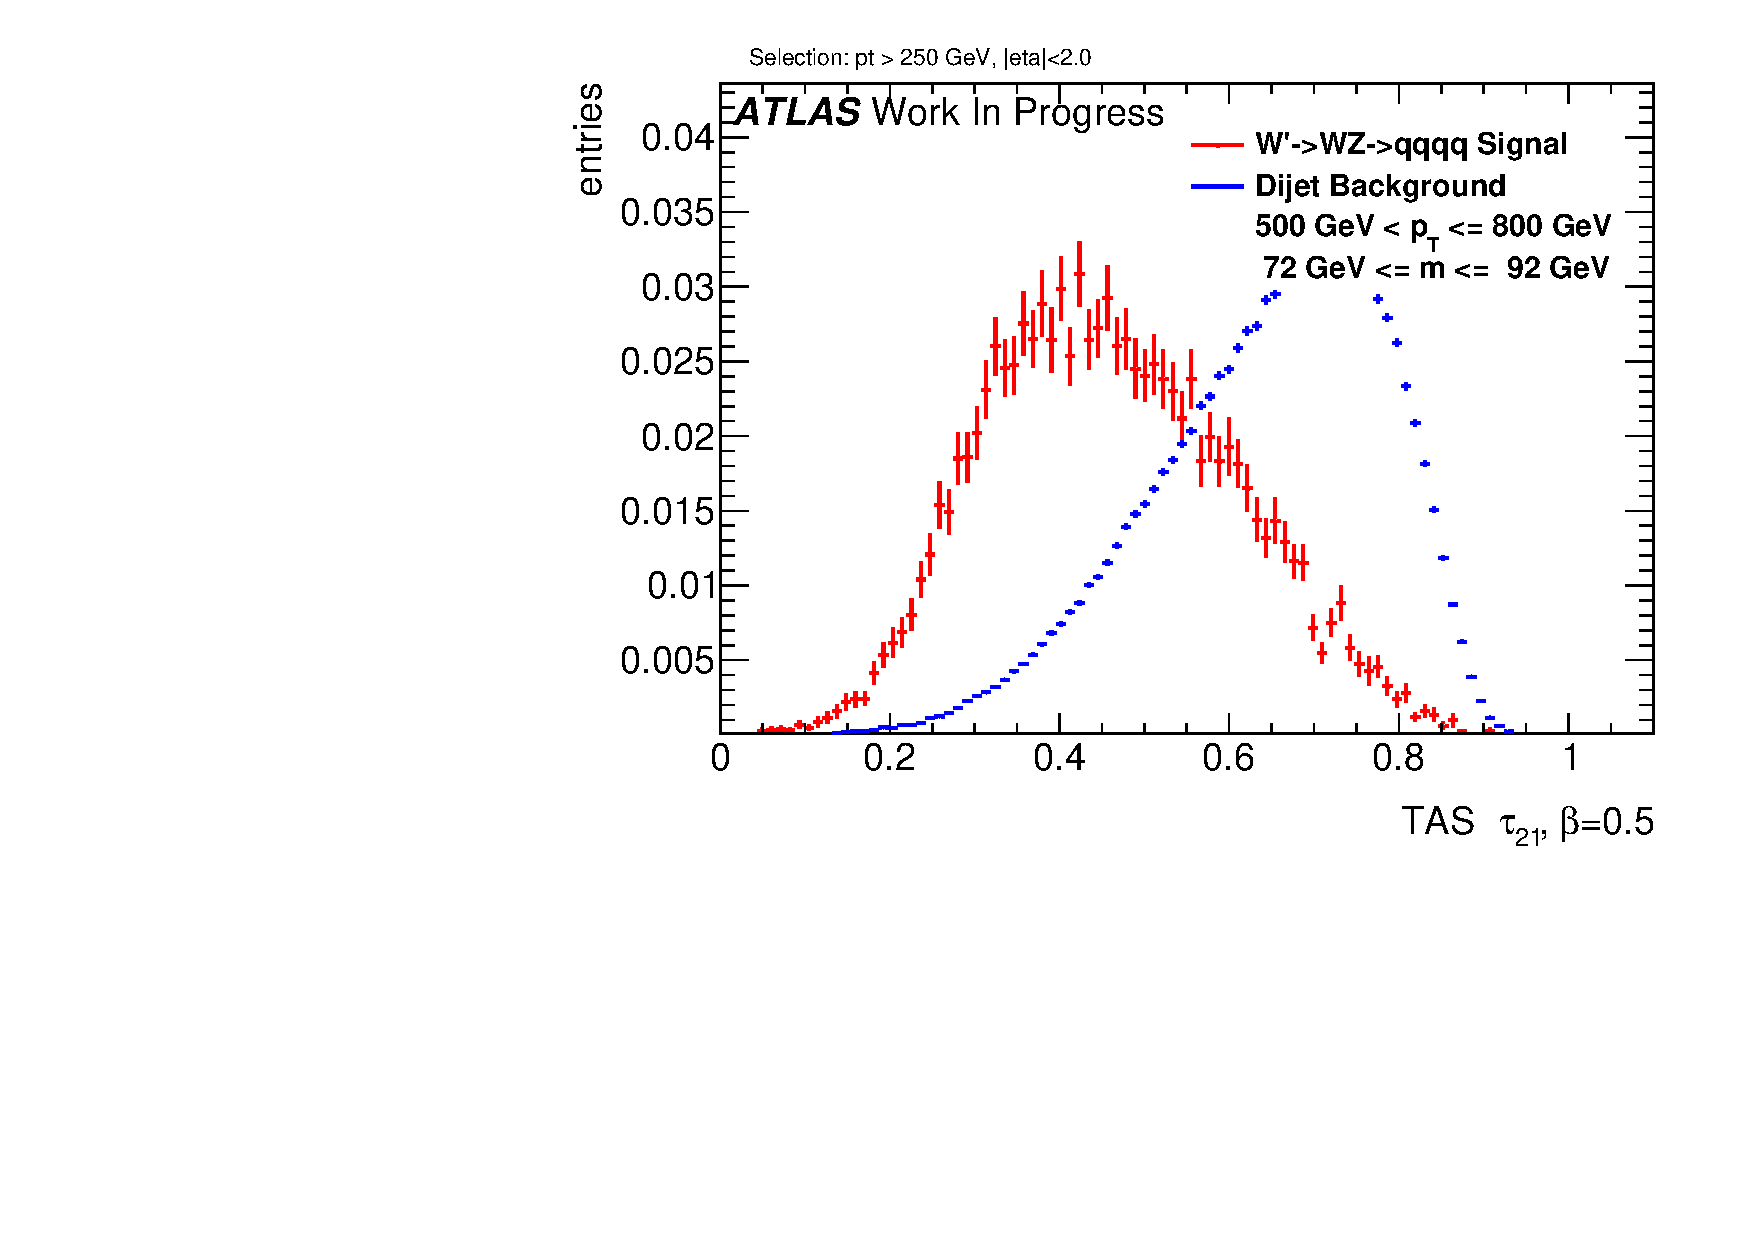
\includegraphics[width=0.3\textwidth]{sascha_input/Appendix/Distributions/w/distributions/beta05/h_assisted_tj_nSub21_05_bin2.pdf} \hspace{1mm}
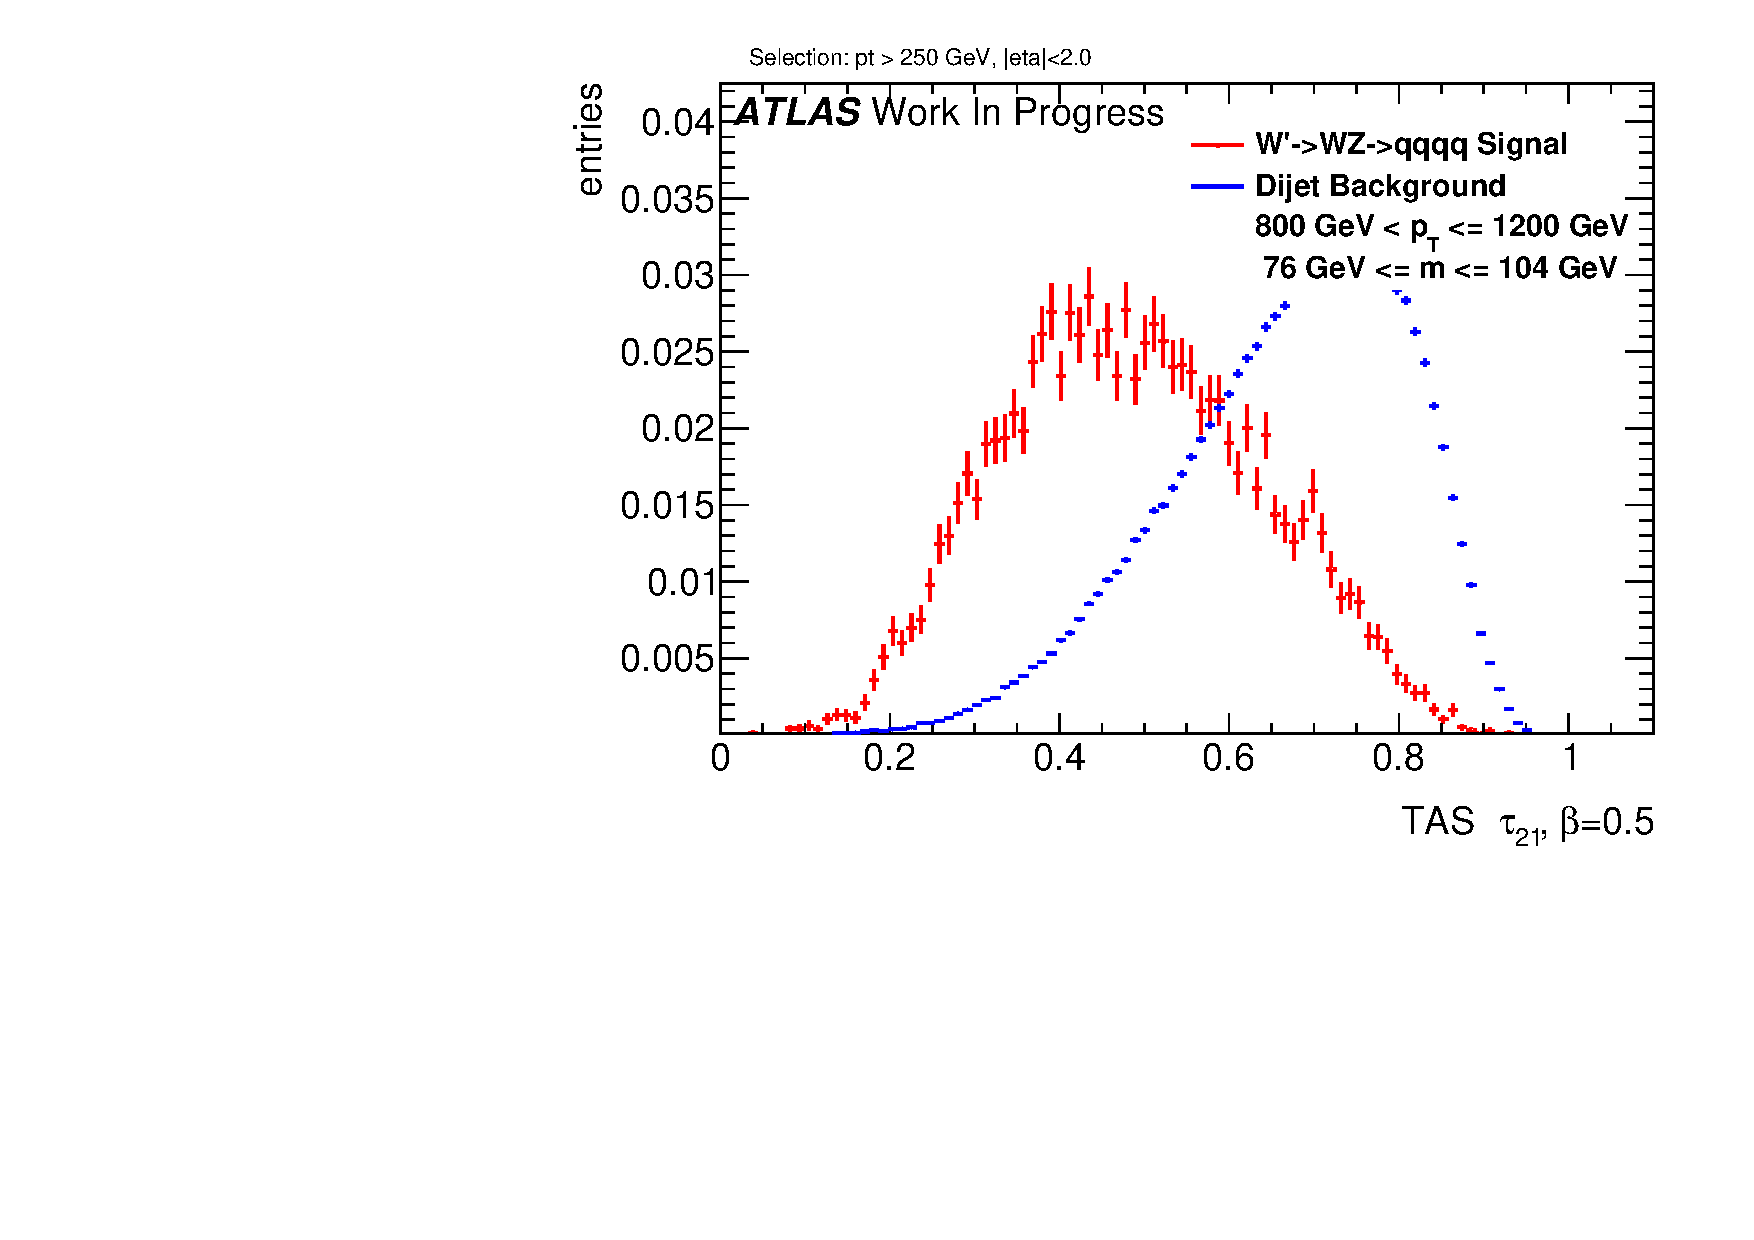
\includegraphics[width=0.3\textwidth]{sascha_input/Appendix/Distributions/w/distributions/beta05/h_assisted_tj_nSub21_05_bin3.pdf} 
\bigskip
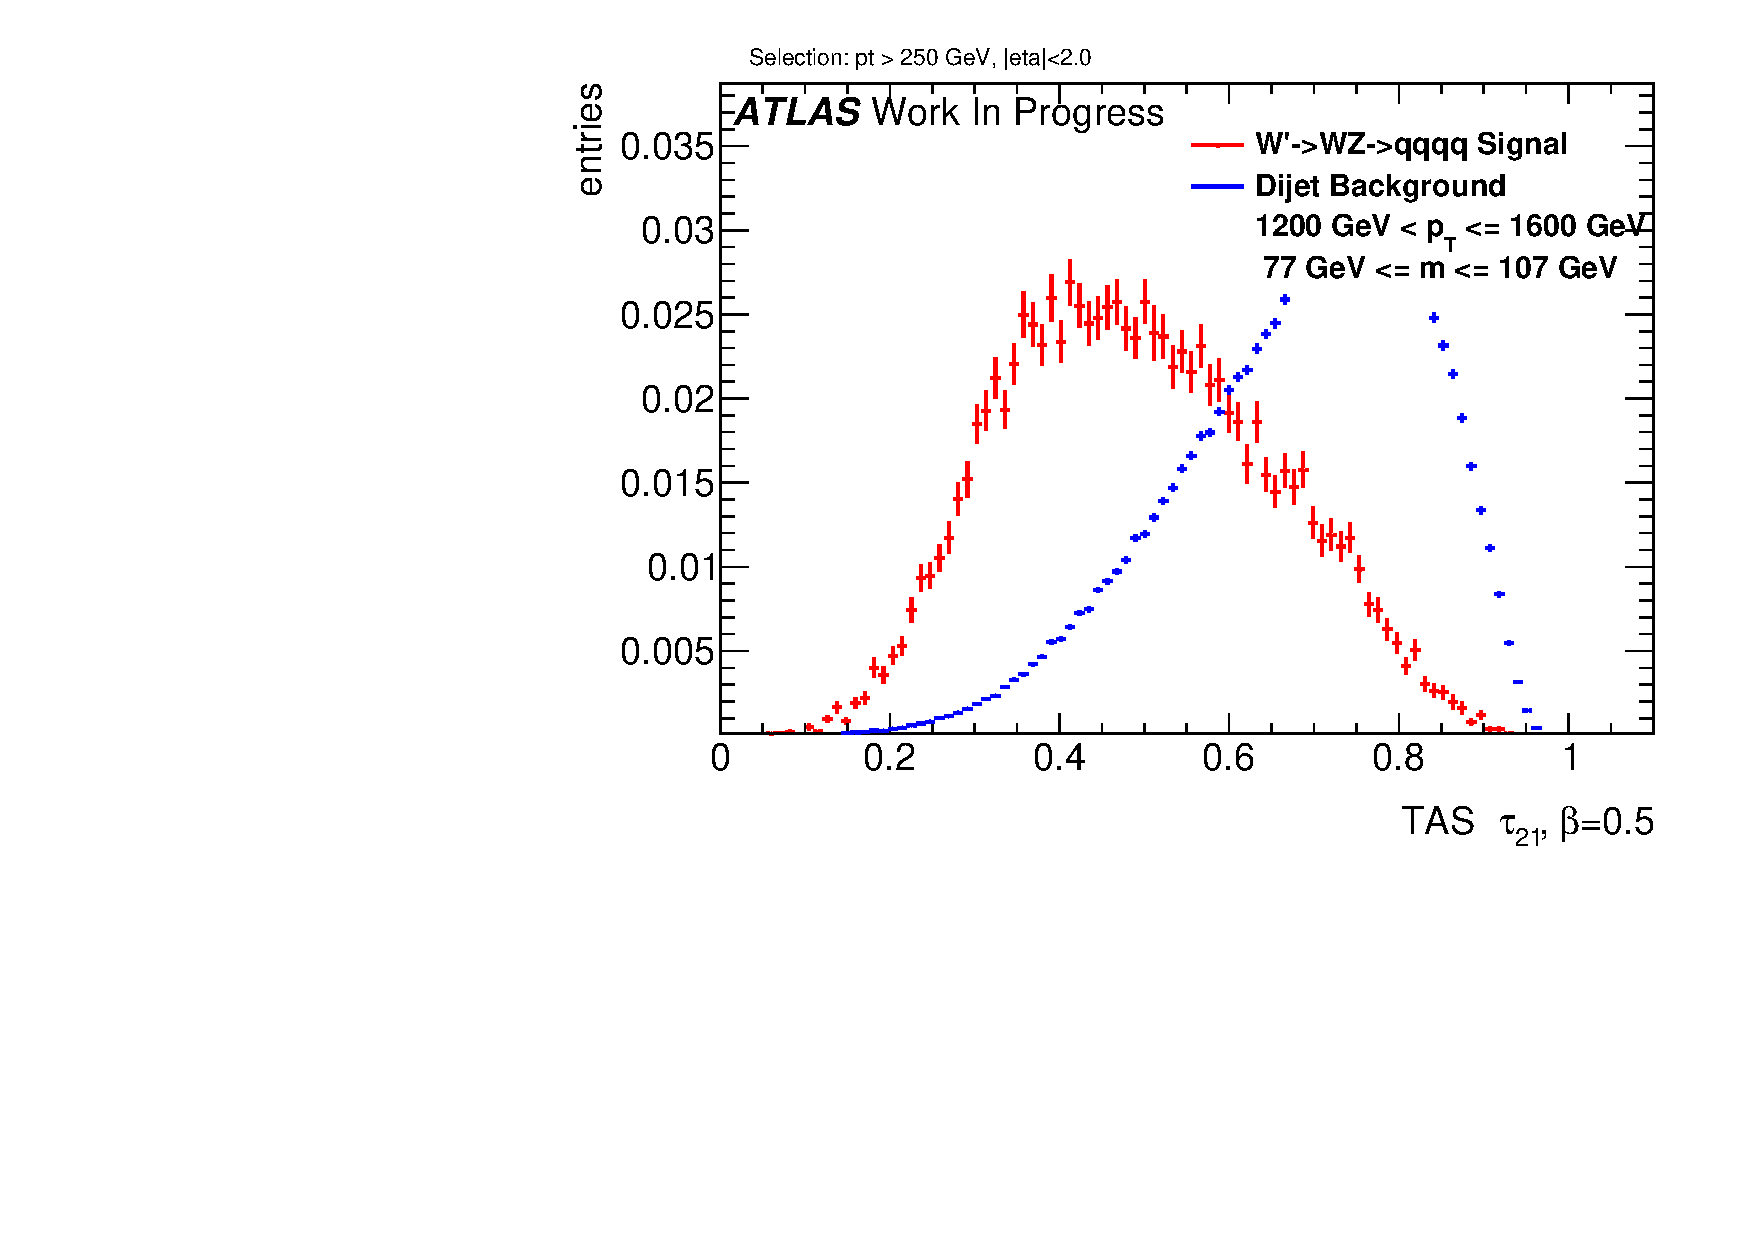
\includegraphics[width=0.3\textwidth]{sascha_input/Appendix/Distributions/w/distributions/beta05/h_assisted_tj_nSub21_05_bin4.pdf} \hspace{6mm}
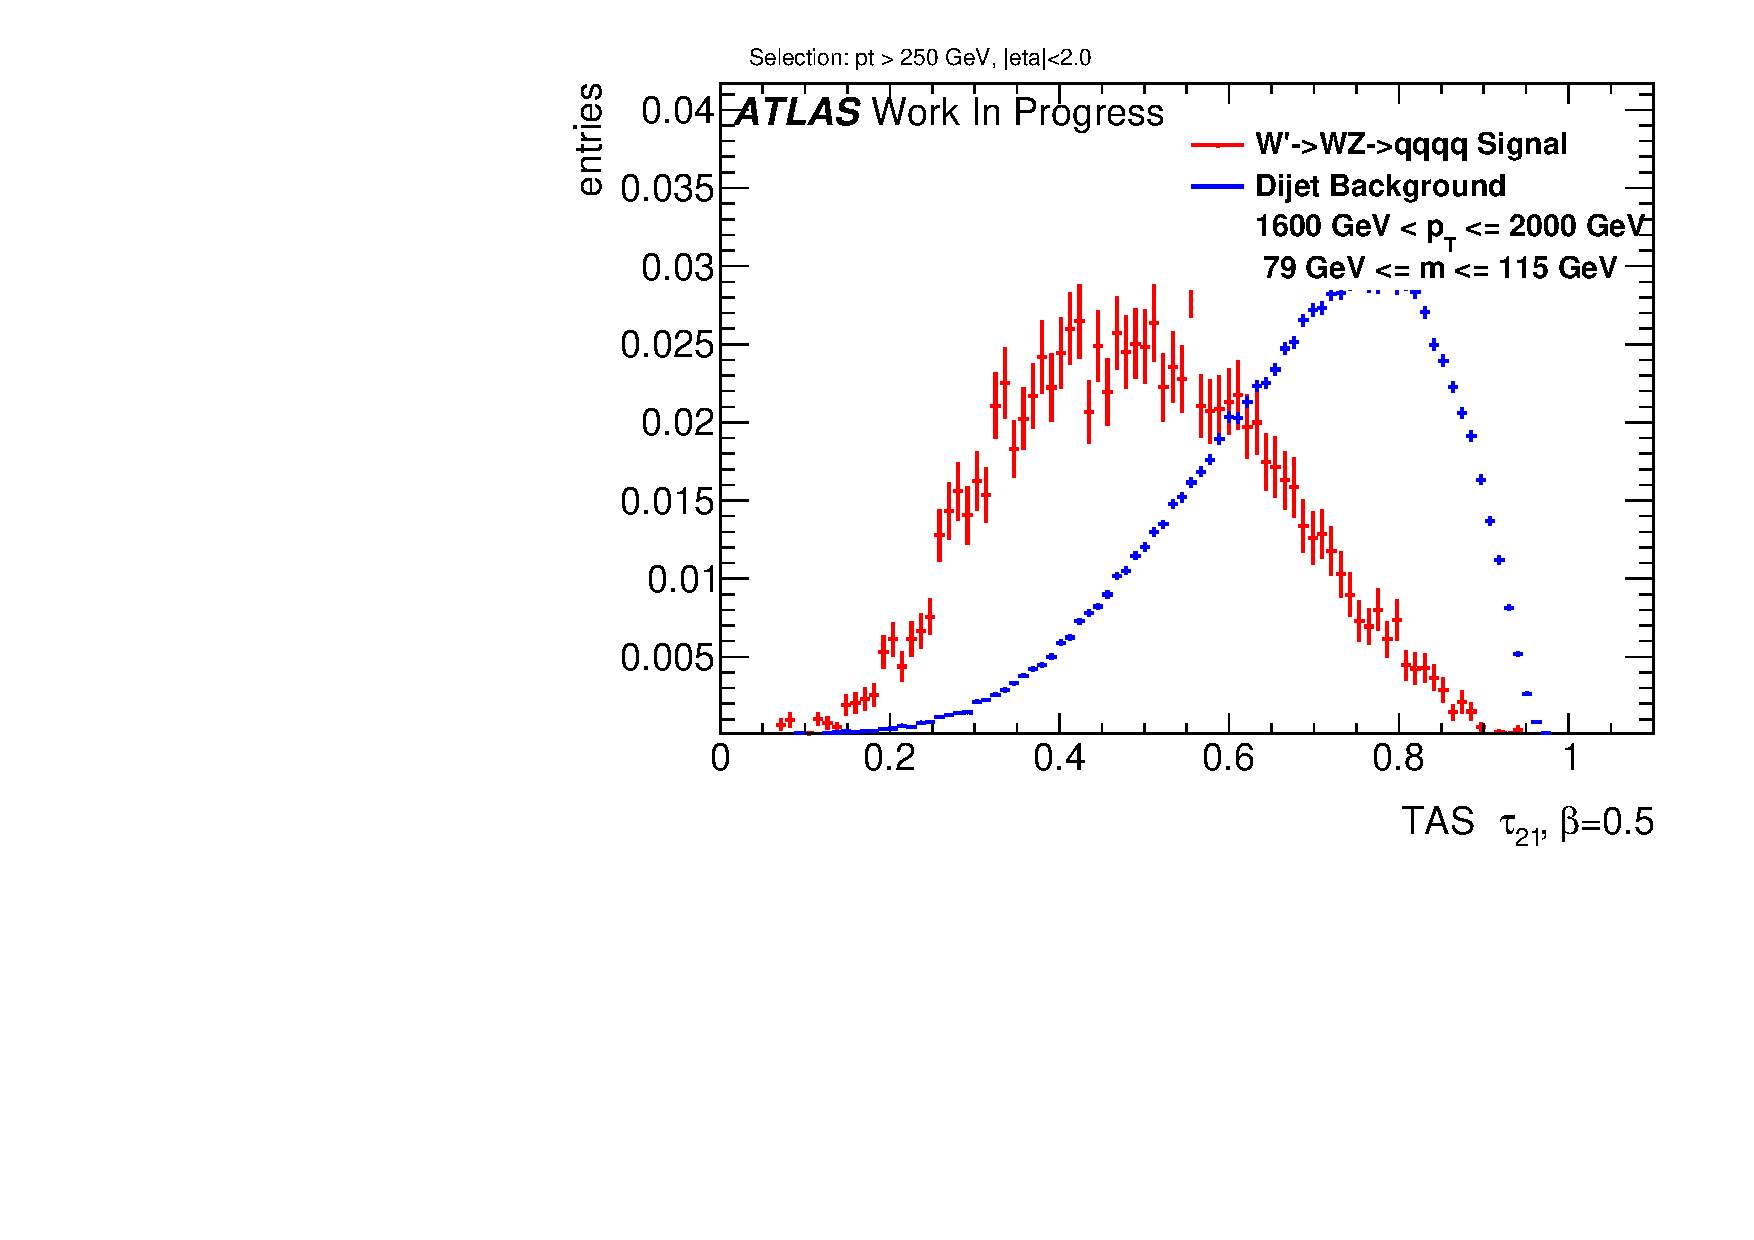
\includegraphics[width=0.3\textwidth]{sascha_input/Appendix/Distributions/w/distributions/beta05/h_assisted_tj_nSub21_05_bin5.pdf} \hspace{6mm}
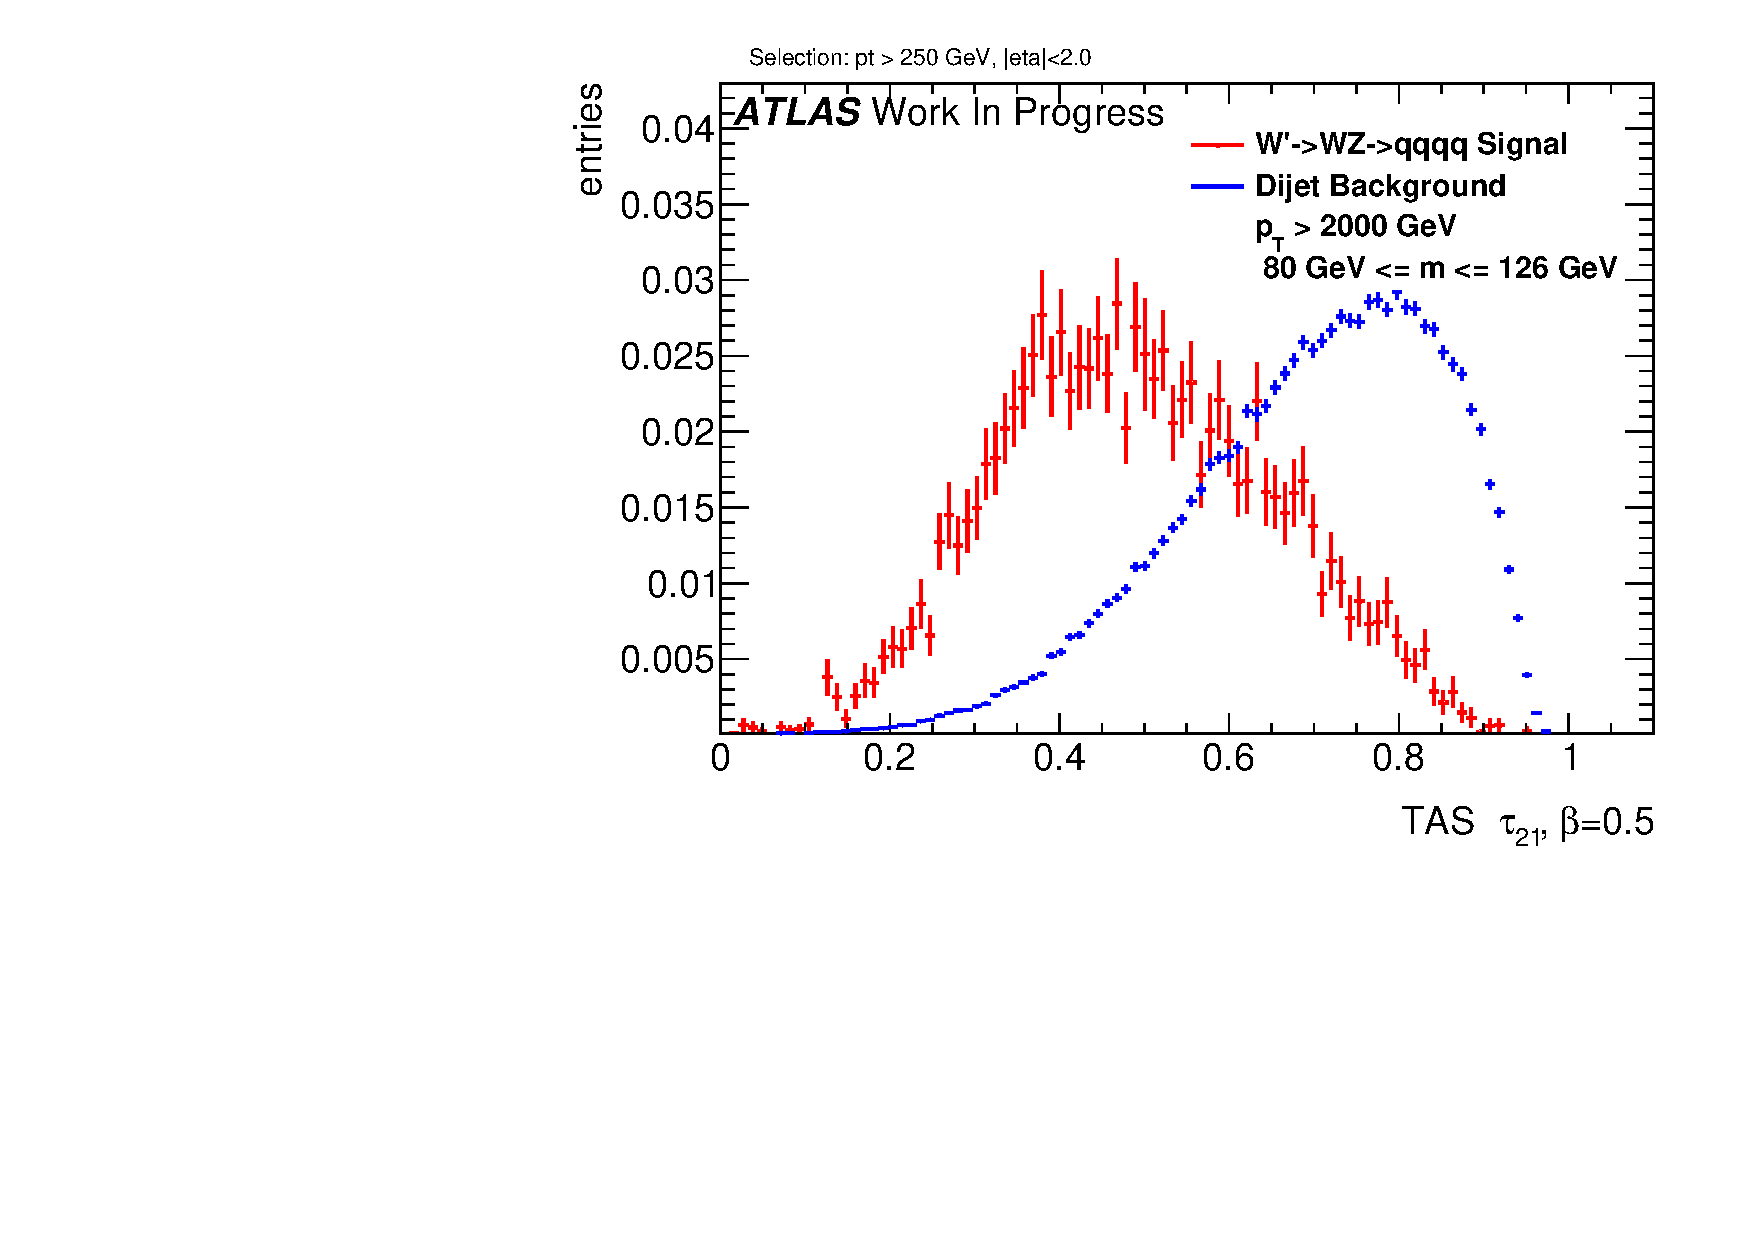
\includegraphics[width=0.3\textwidth]{sascha_input/Appendix/Distributions/w/distributions/beta05/h_assisted_tj_nSub21_05_bin6.pdf} 
\vspace{-1.25cm}
\caption{{Distributions for $W$ boson tagging using TAS $\beta=0.5$. C2, D2, $\tau_{21}$ top down.}}
\end{figure}
\begin{figure}[H]
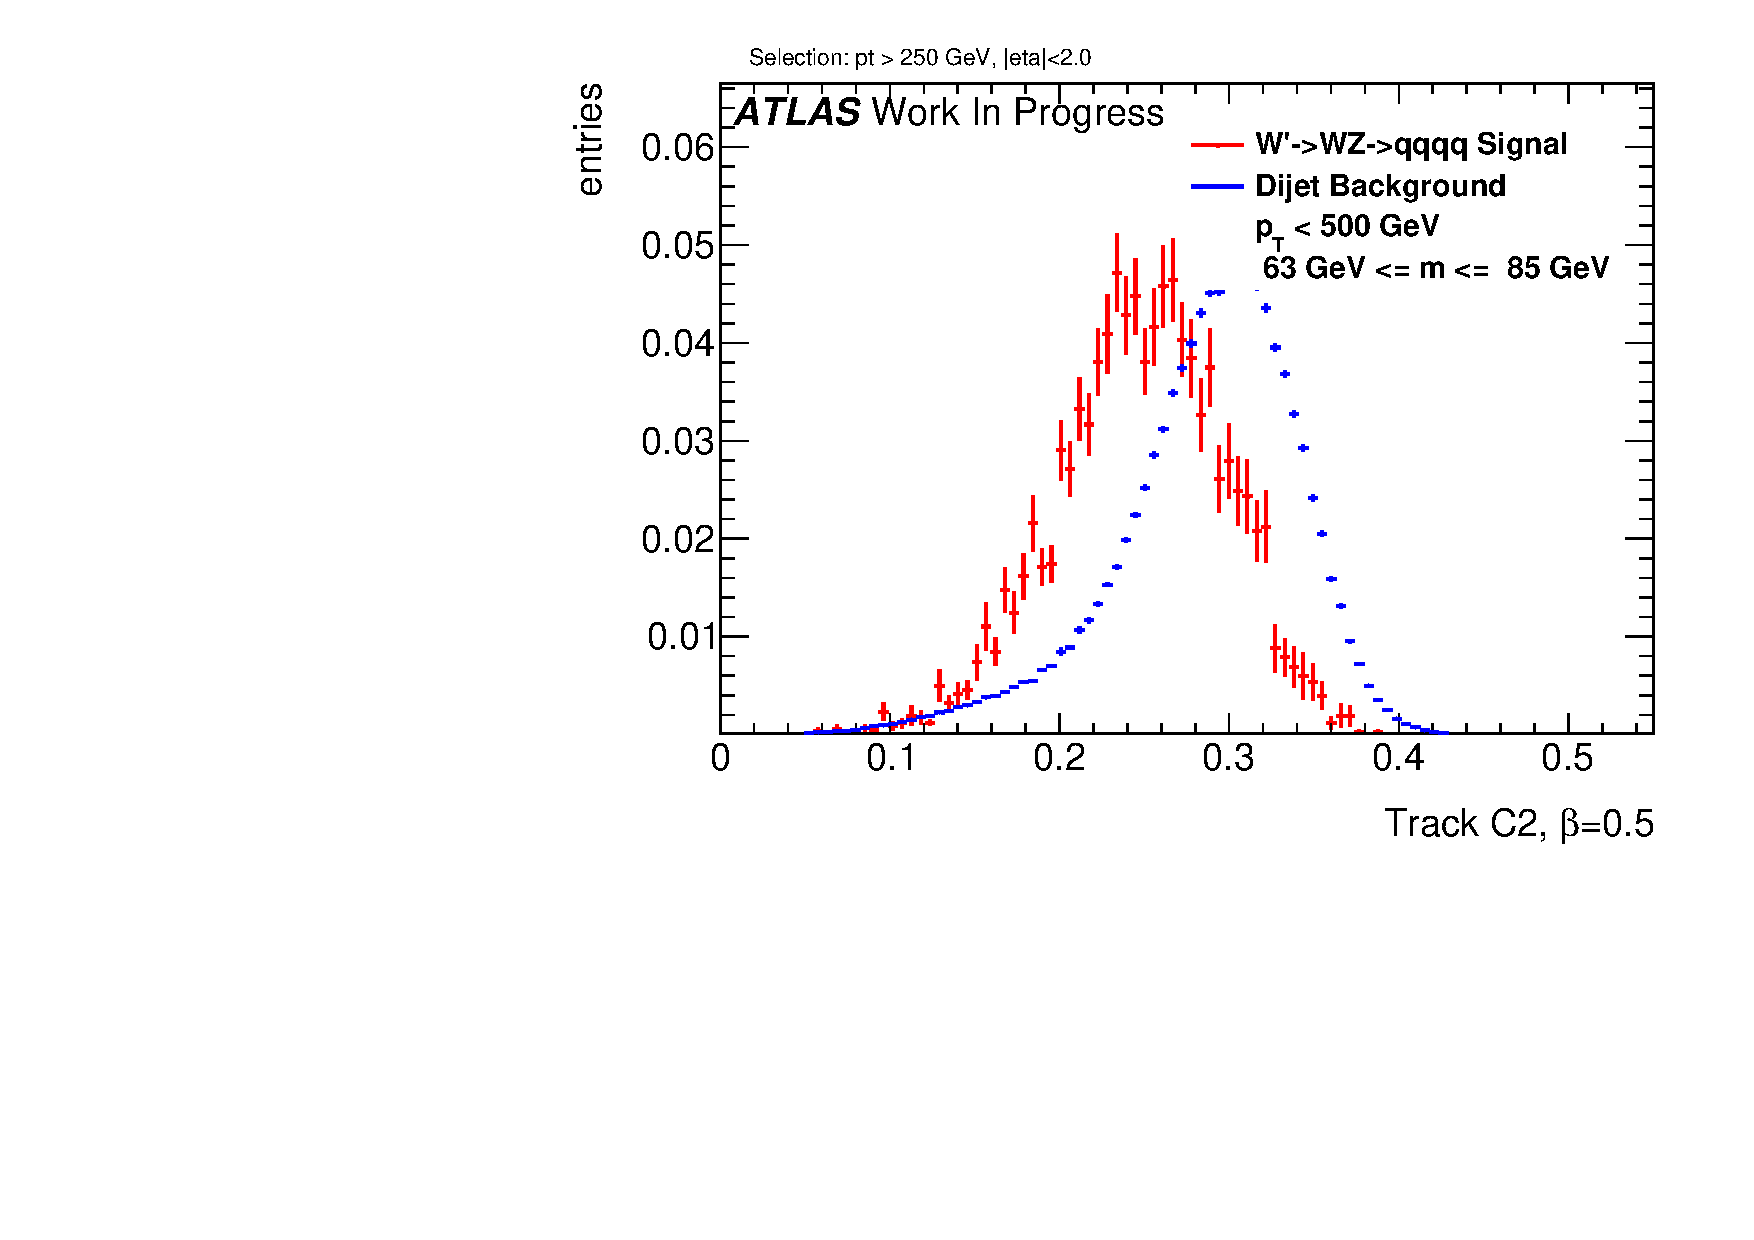
\includegraphics[width=0.3\textwidth]{sascha_input/Appendix/Distributions/w/distributions/beta05/h_normal_tj_C2_05_bin1.pdf} \hspace{1mm}
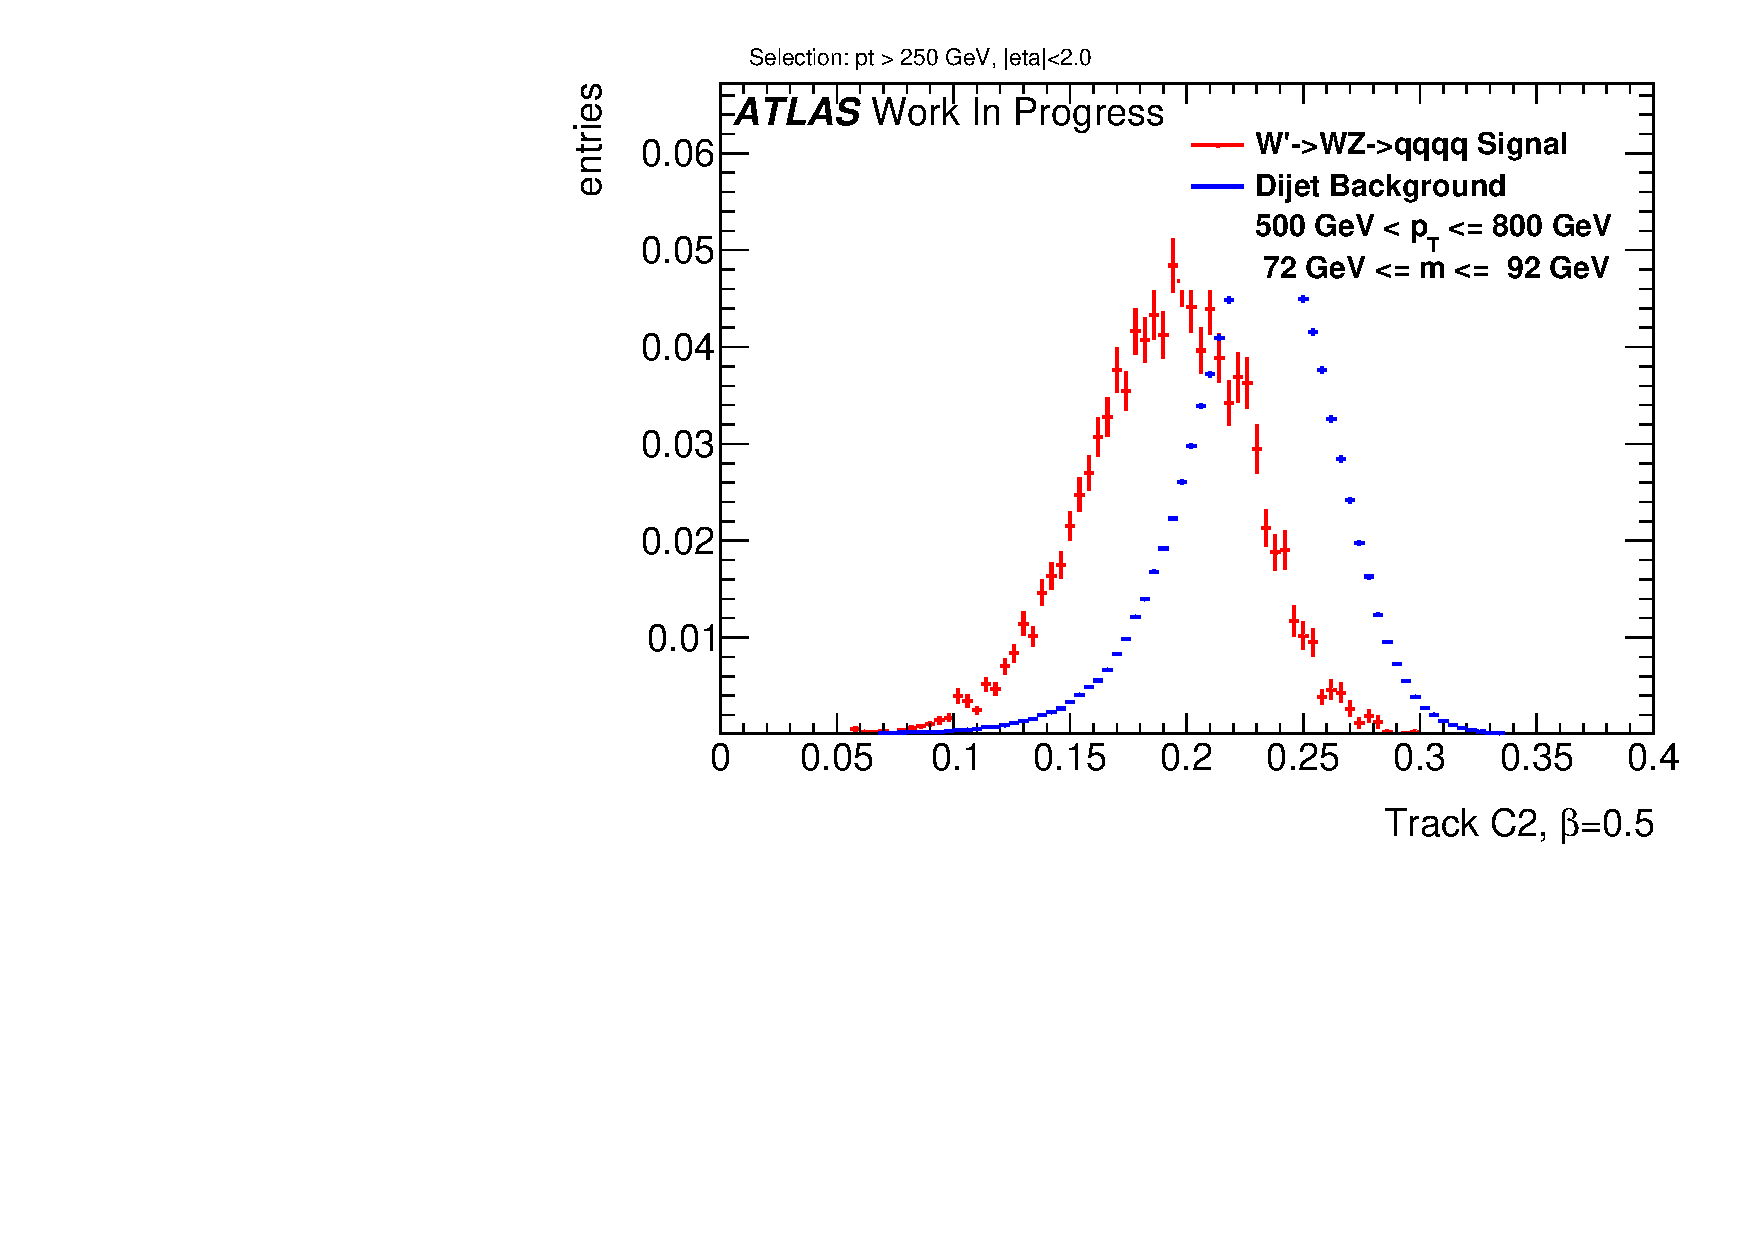
\includegraphics[width=0.3\textwidth]{sascha_input/Appendix/Distributions/w/distributions/beta05/h_normal_tj_C2_05_bin2.pdf} \hspace{1mm}
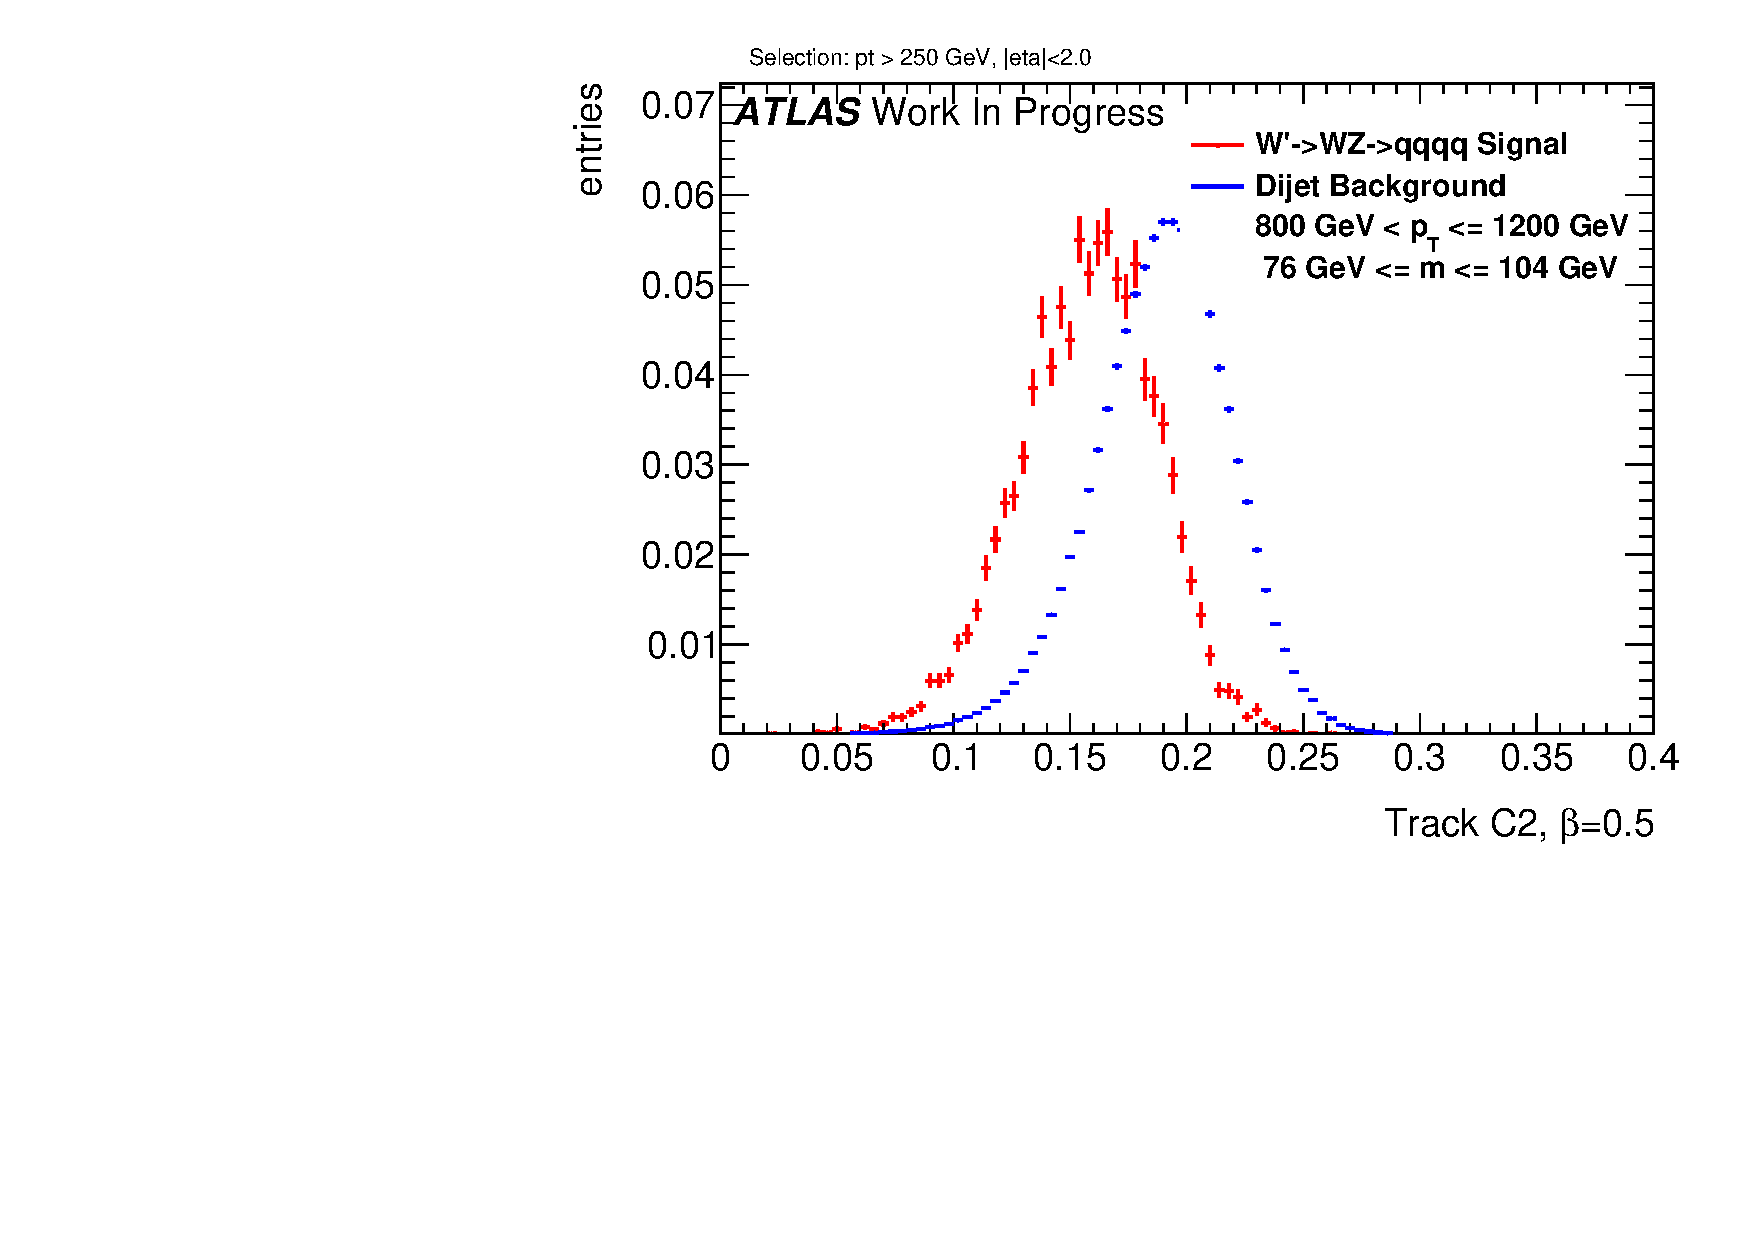
\includegraphics[width=0.3\textwidth]{sascha_input/Appendix/Distributions/w/distributions/beta05/h_normal_tj_C2_05_bin3.pdf} 
\bigskip
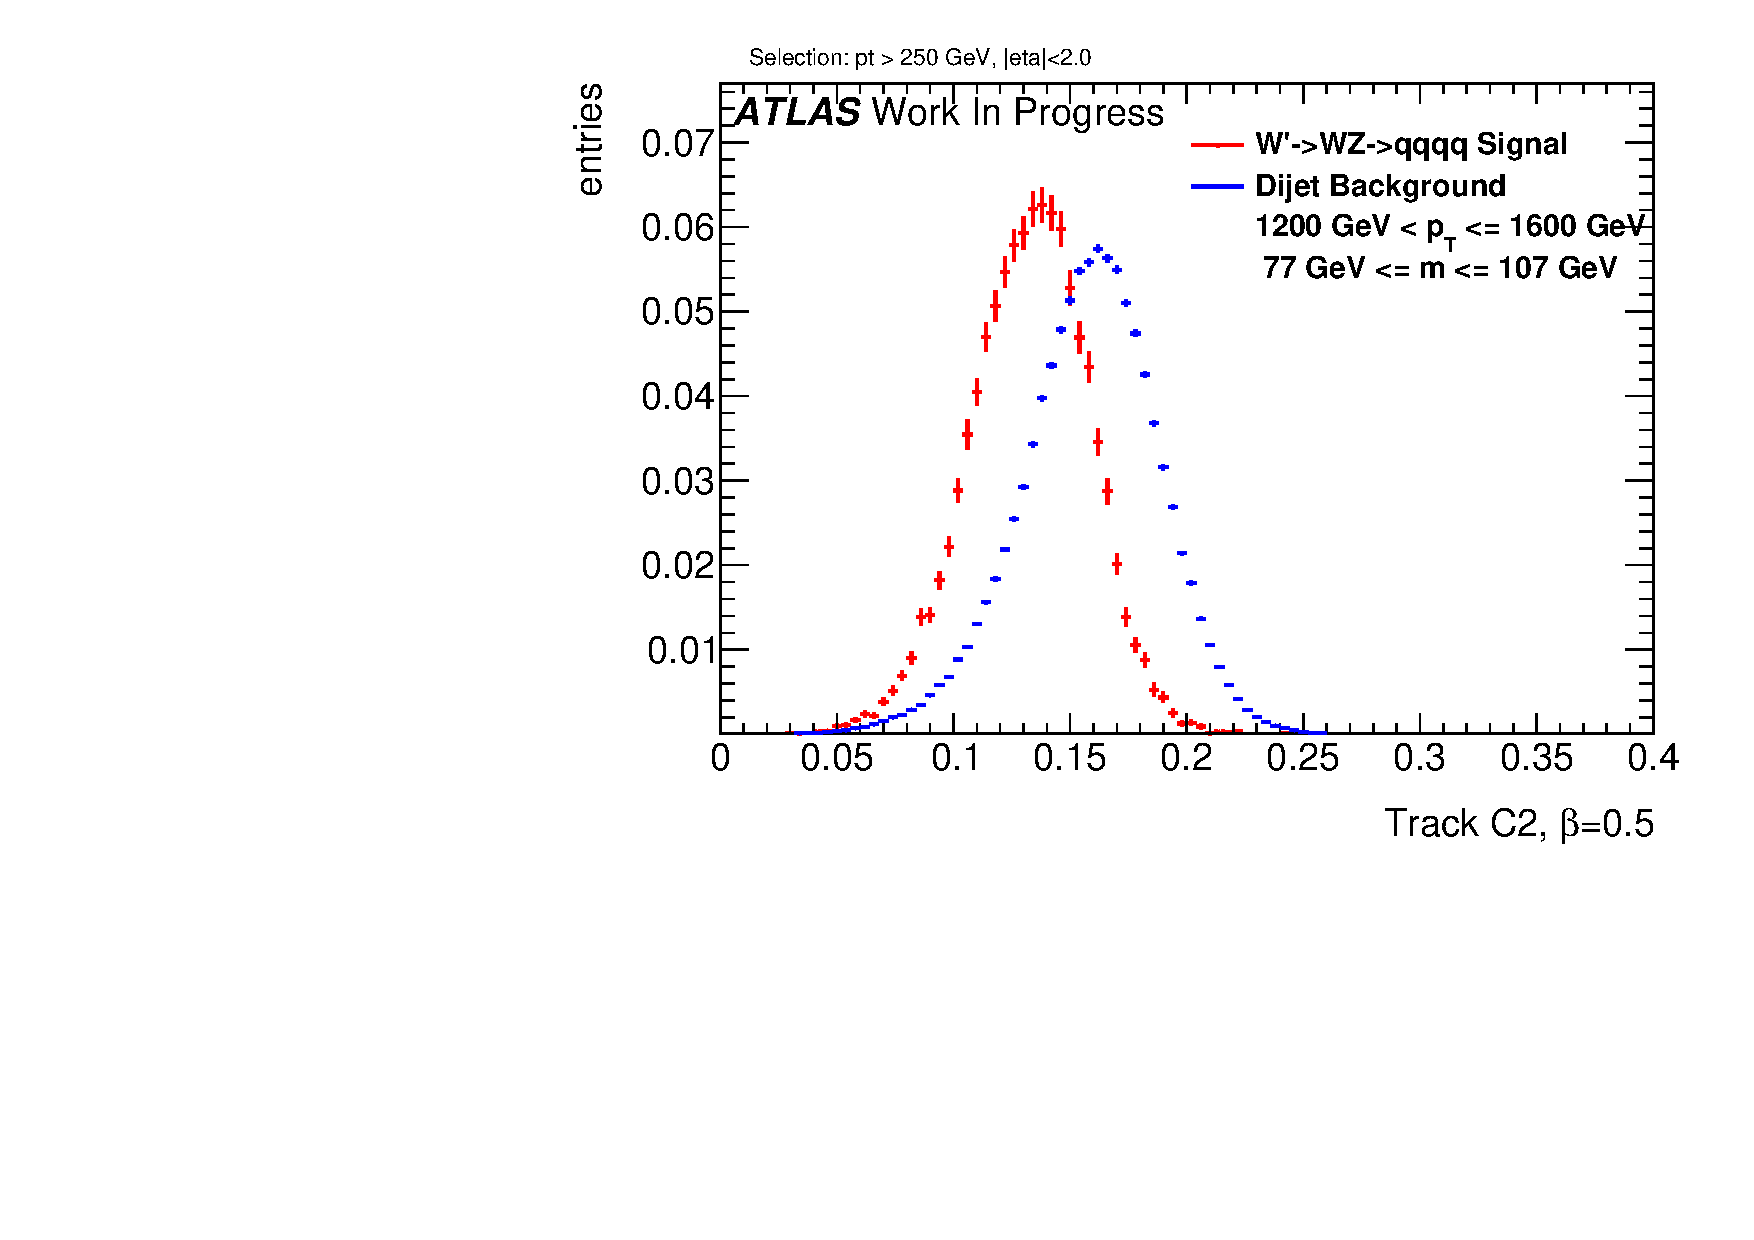
\includegraphics[width=0.3\textwidth]{sascha_input/Appendix/Distributions/w/distributions/beta05/h_normal_tj_C2_05_bin4.pdf} \hspace{1mm}
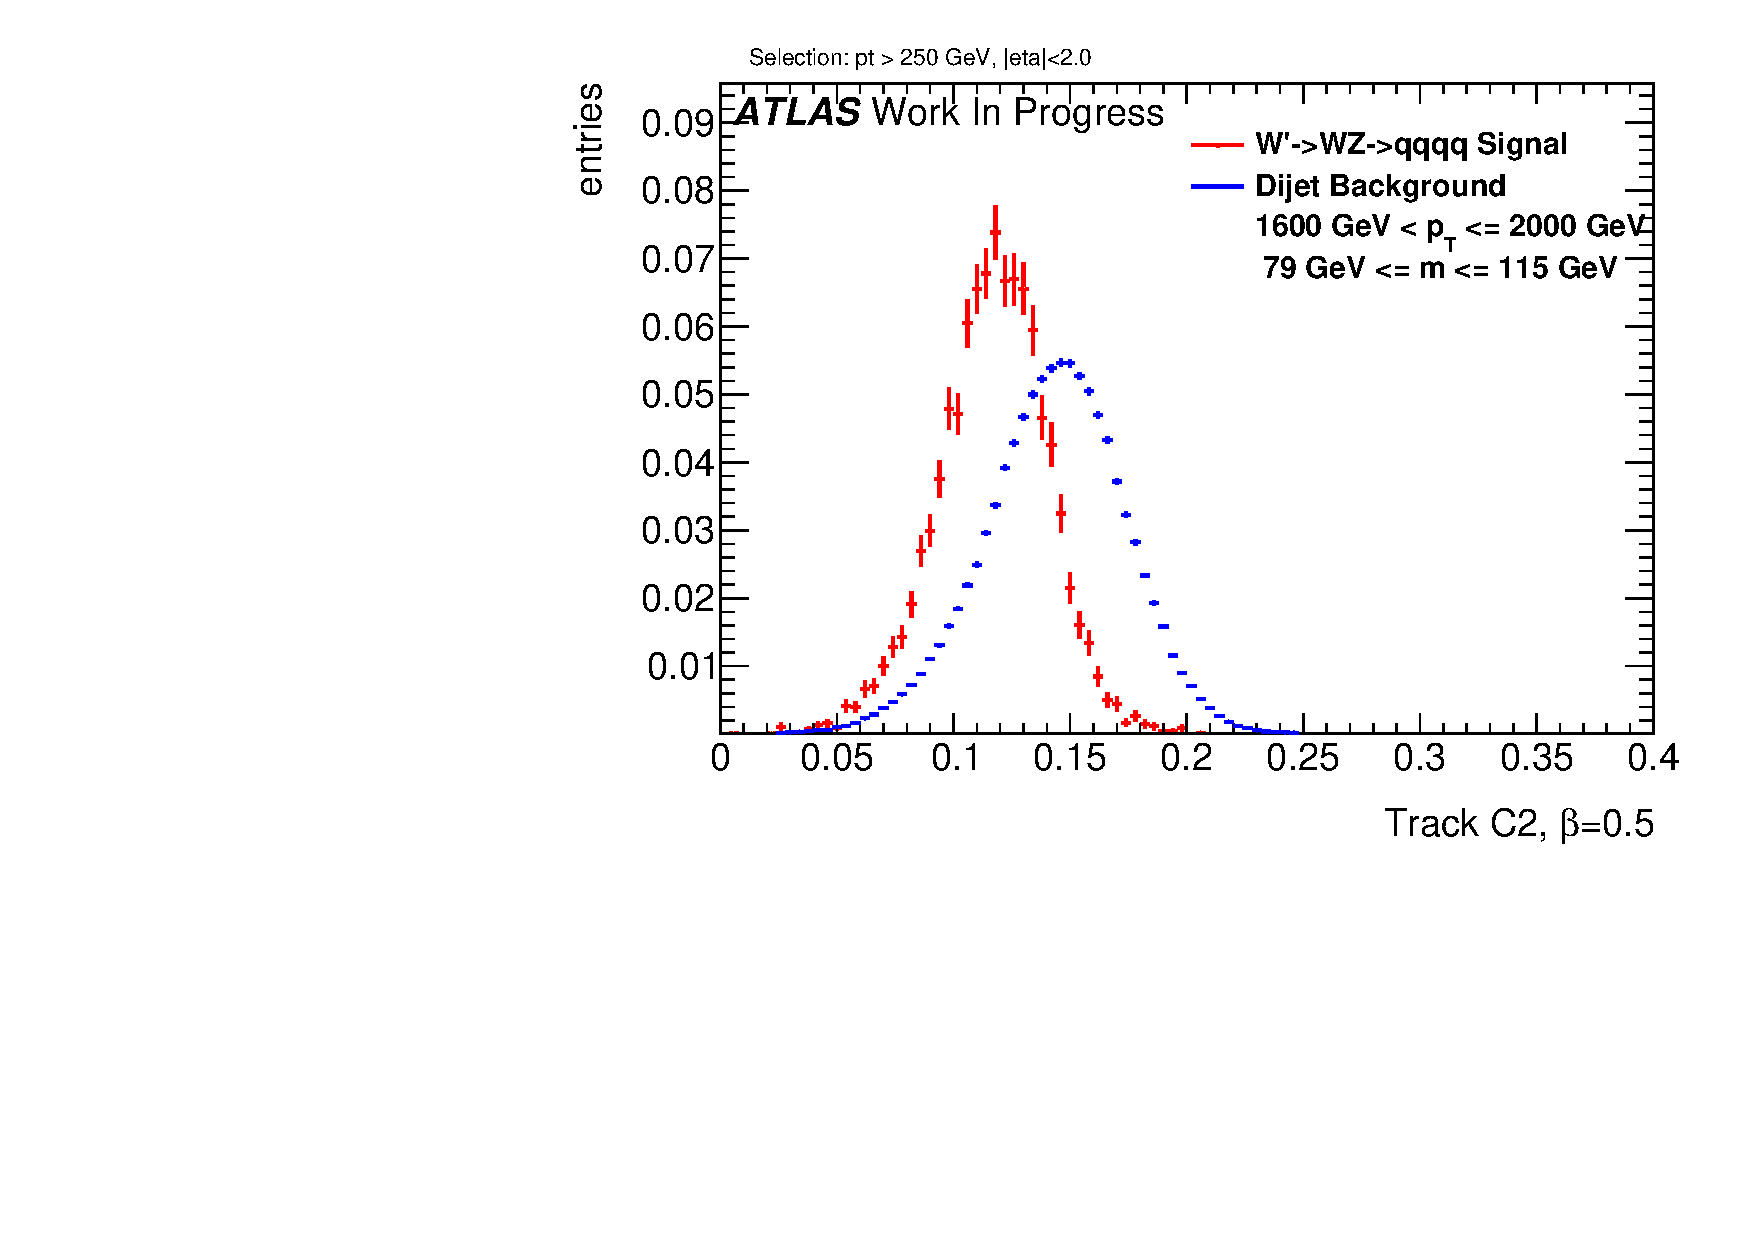
\includegraphics[width=0.3\textwidth]{sascha_input/Appendix/Distributions/w/distributions/beta05/h_normal_tj_C2_05_bin5.pdf} \hspace{1mm}
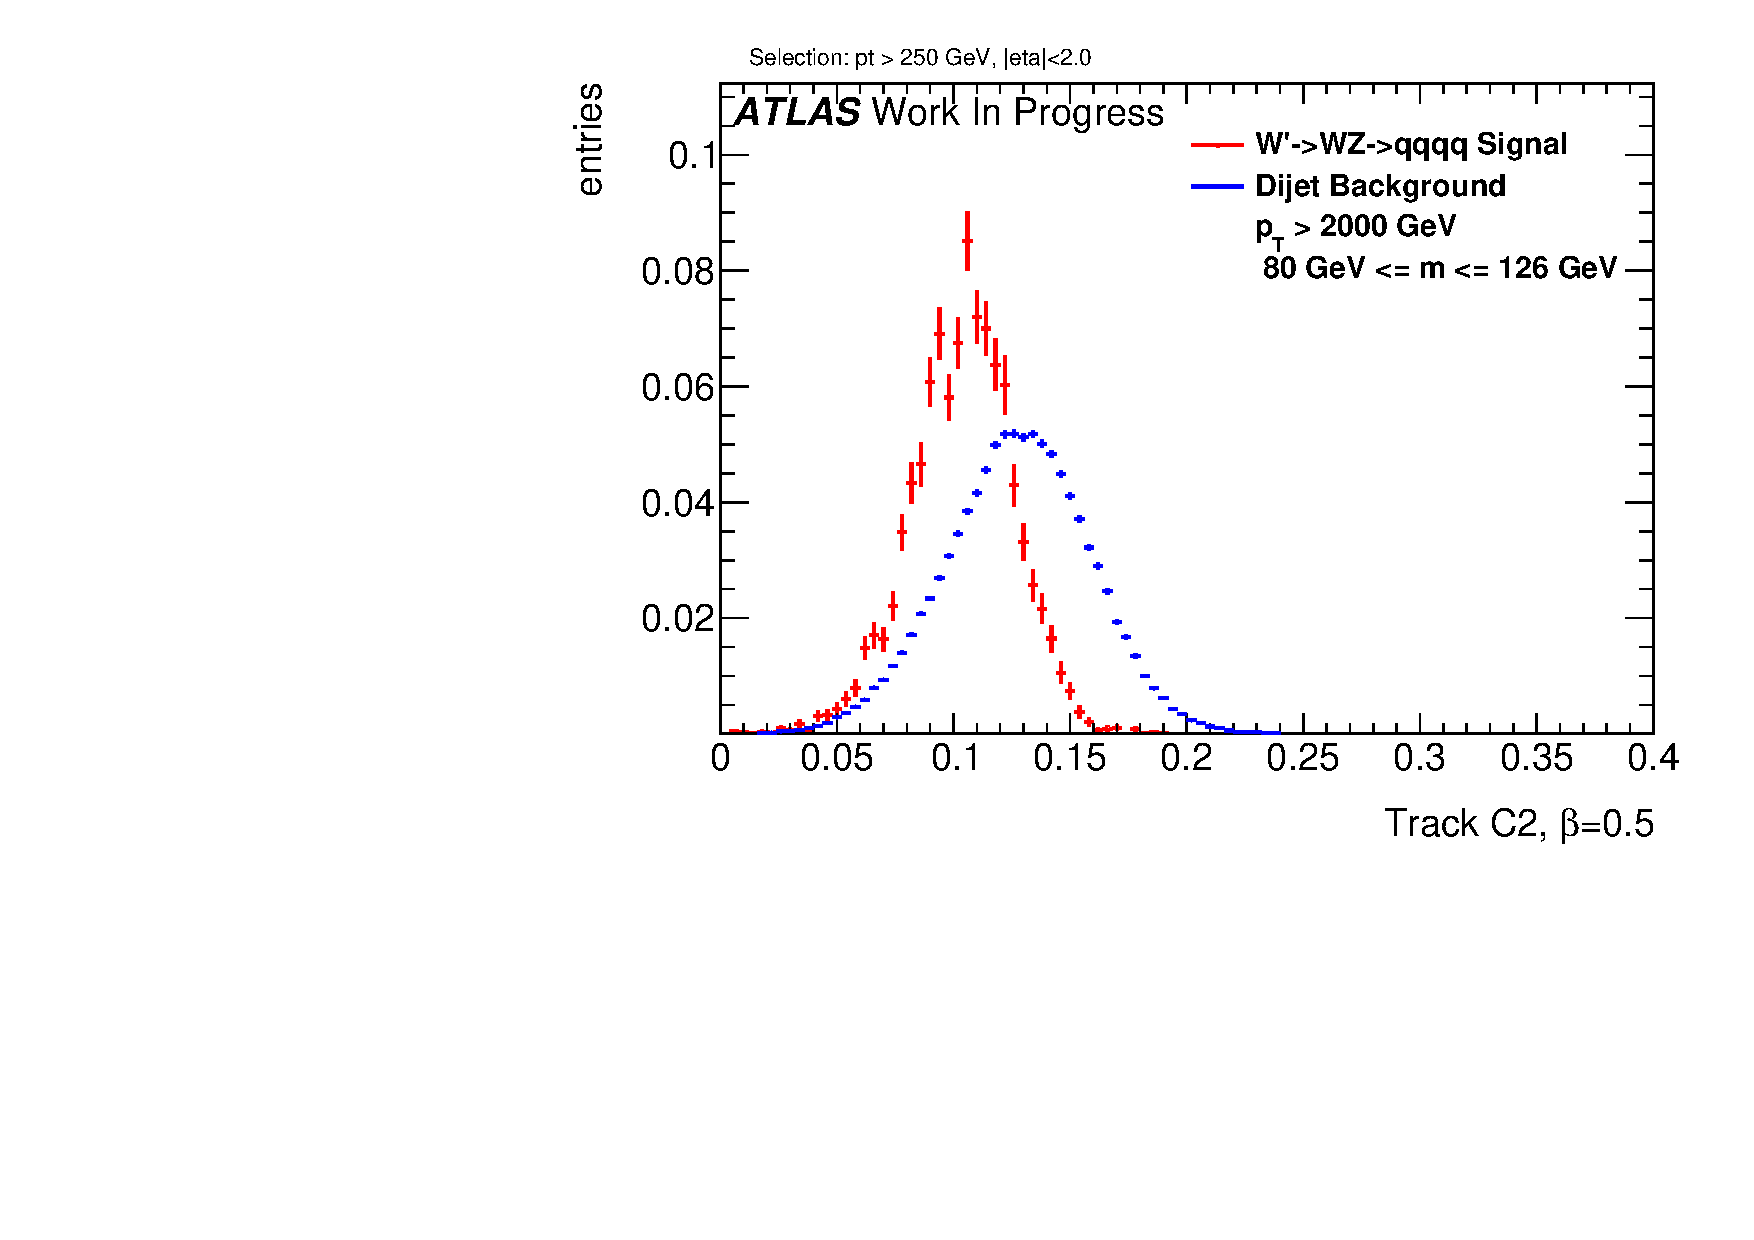
\includegraphics[width=0.3\textwidth]{sascha_input/Appendix/Distributions/w/distributions/beta05/h_normal_tj_C2_05_bin6.pdf} 
\bigskip
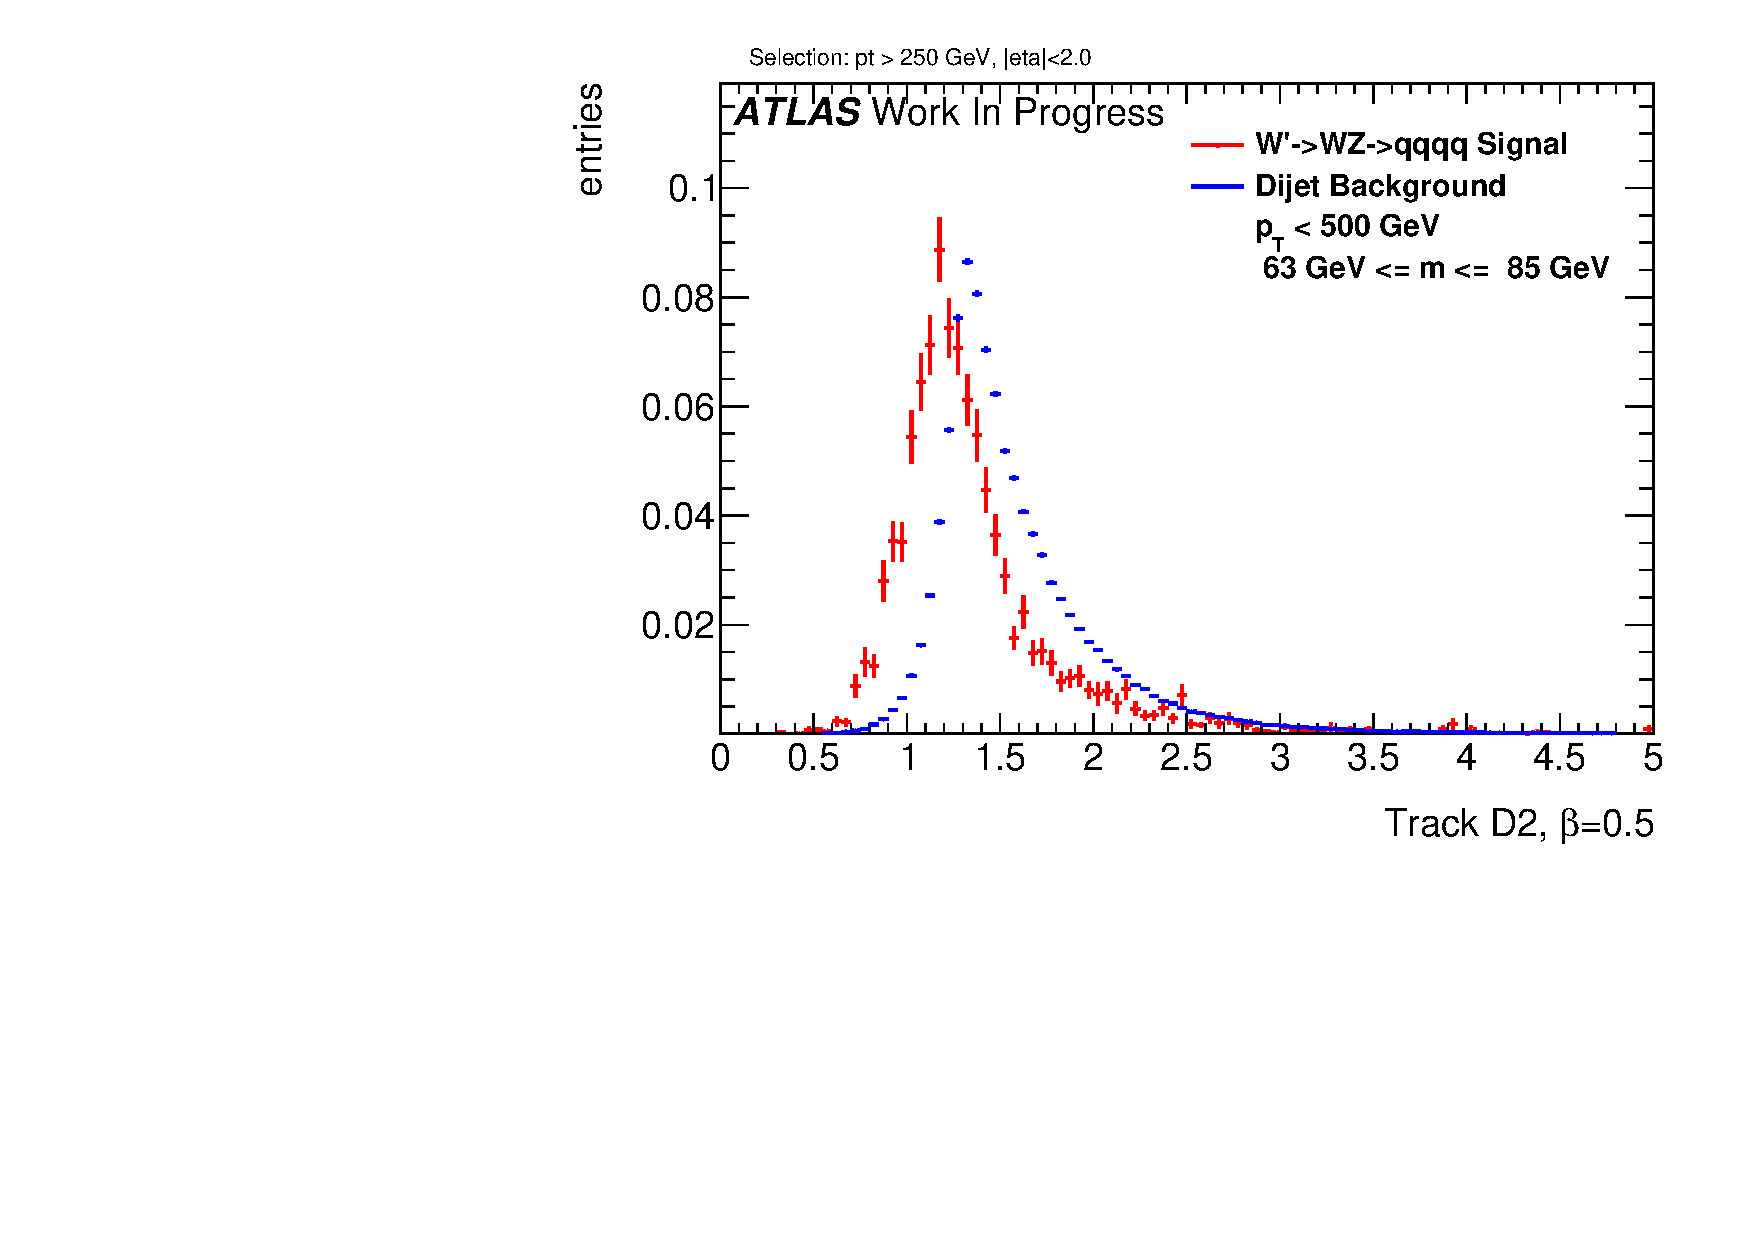
\includegraphics[width=0.3\textwidth]{sascha_input/Appendix/Distributions/w/distributions/beta05/h_normal_tj_D2_05_bin1.pdf} \hspace{1mm}
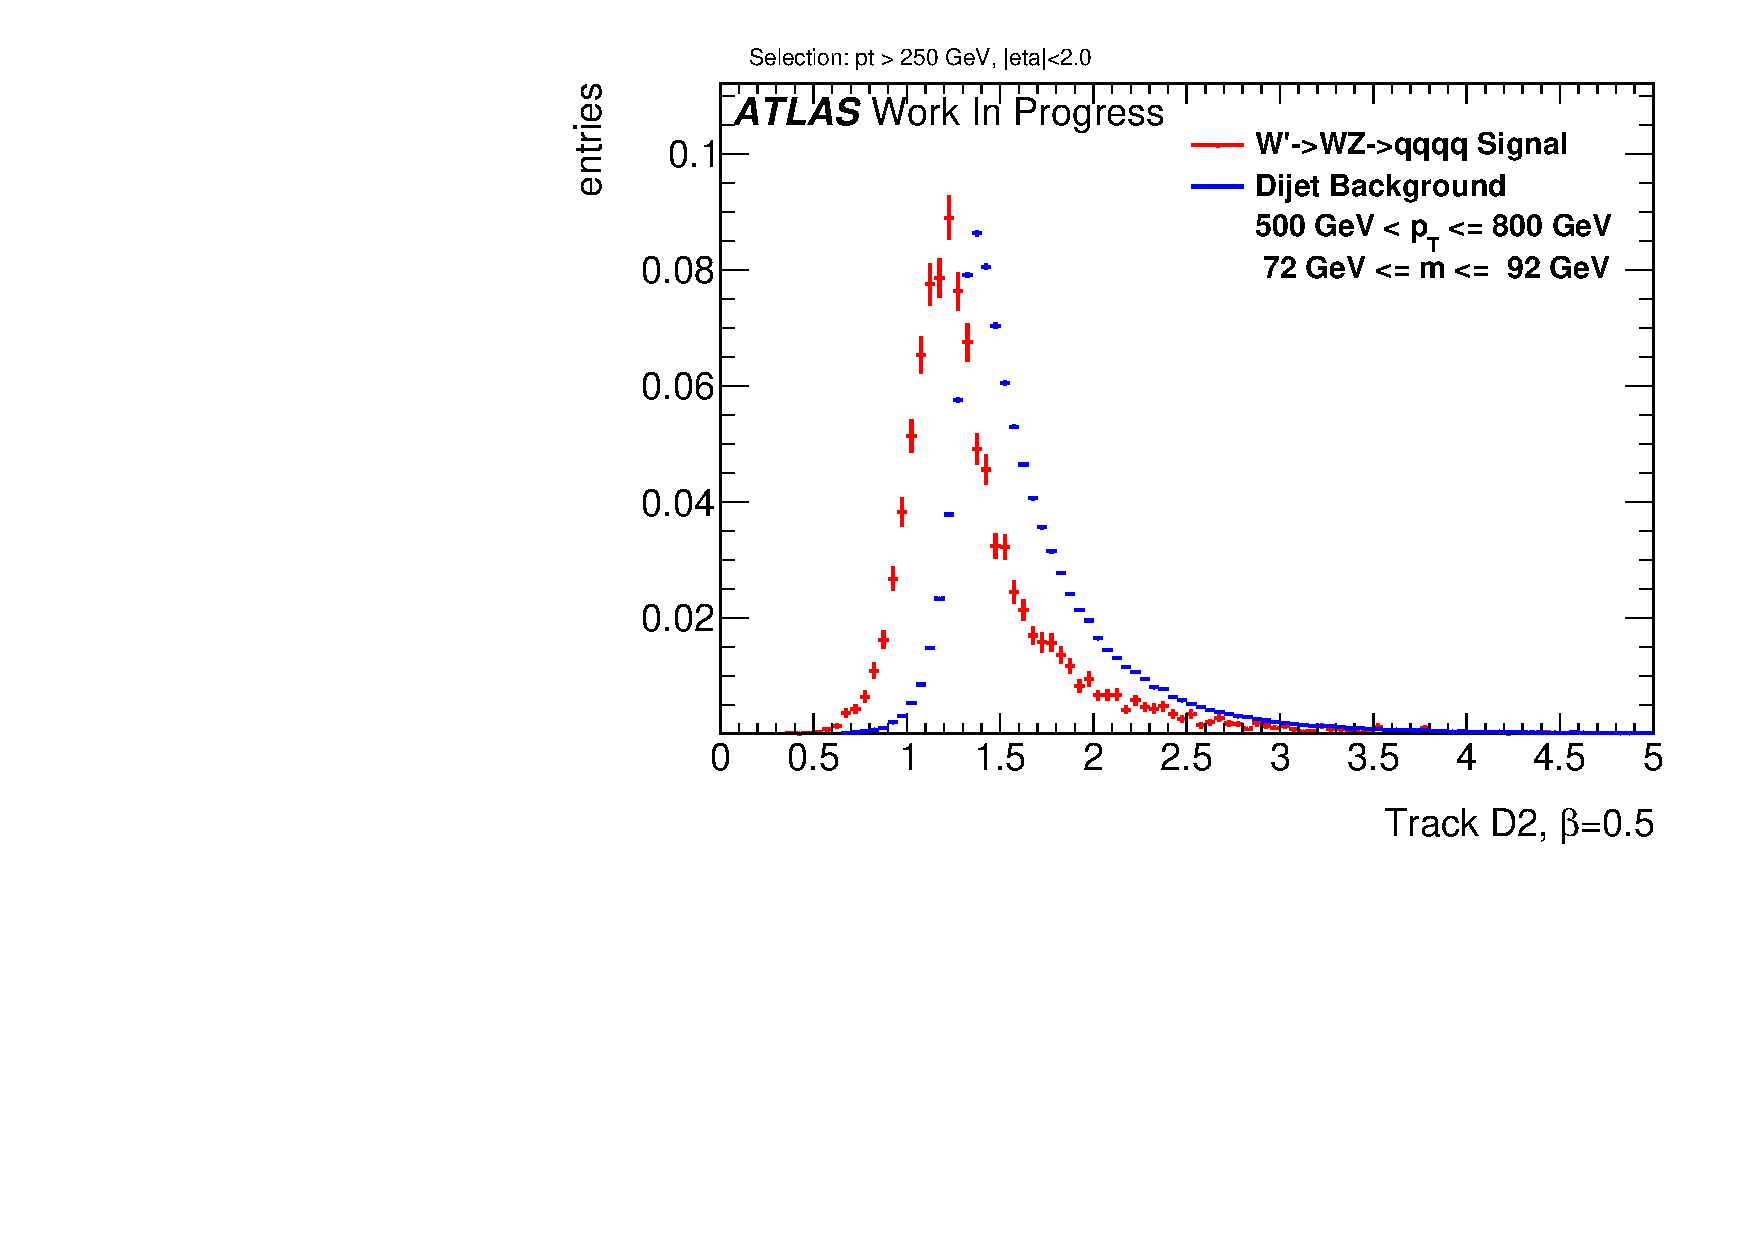
\includegraphics[width=0.3\textwidth]{sascha_input/Appendix/Distributions/w/distributions/beta05/h_normal_tj_D2_05_bin2.pdf} \hspace{1mm}
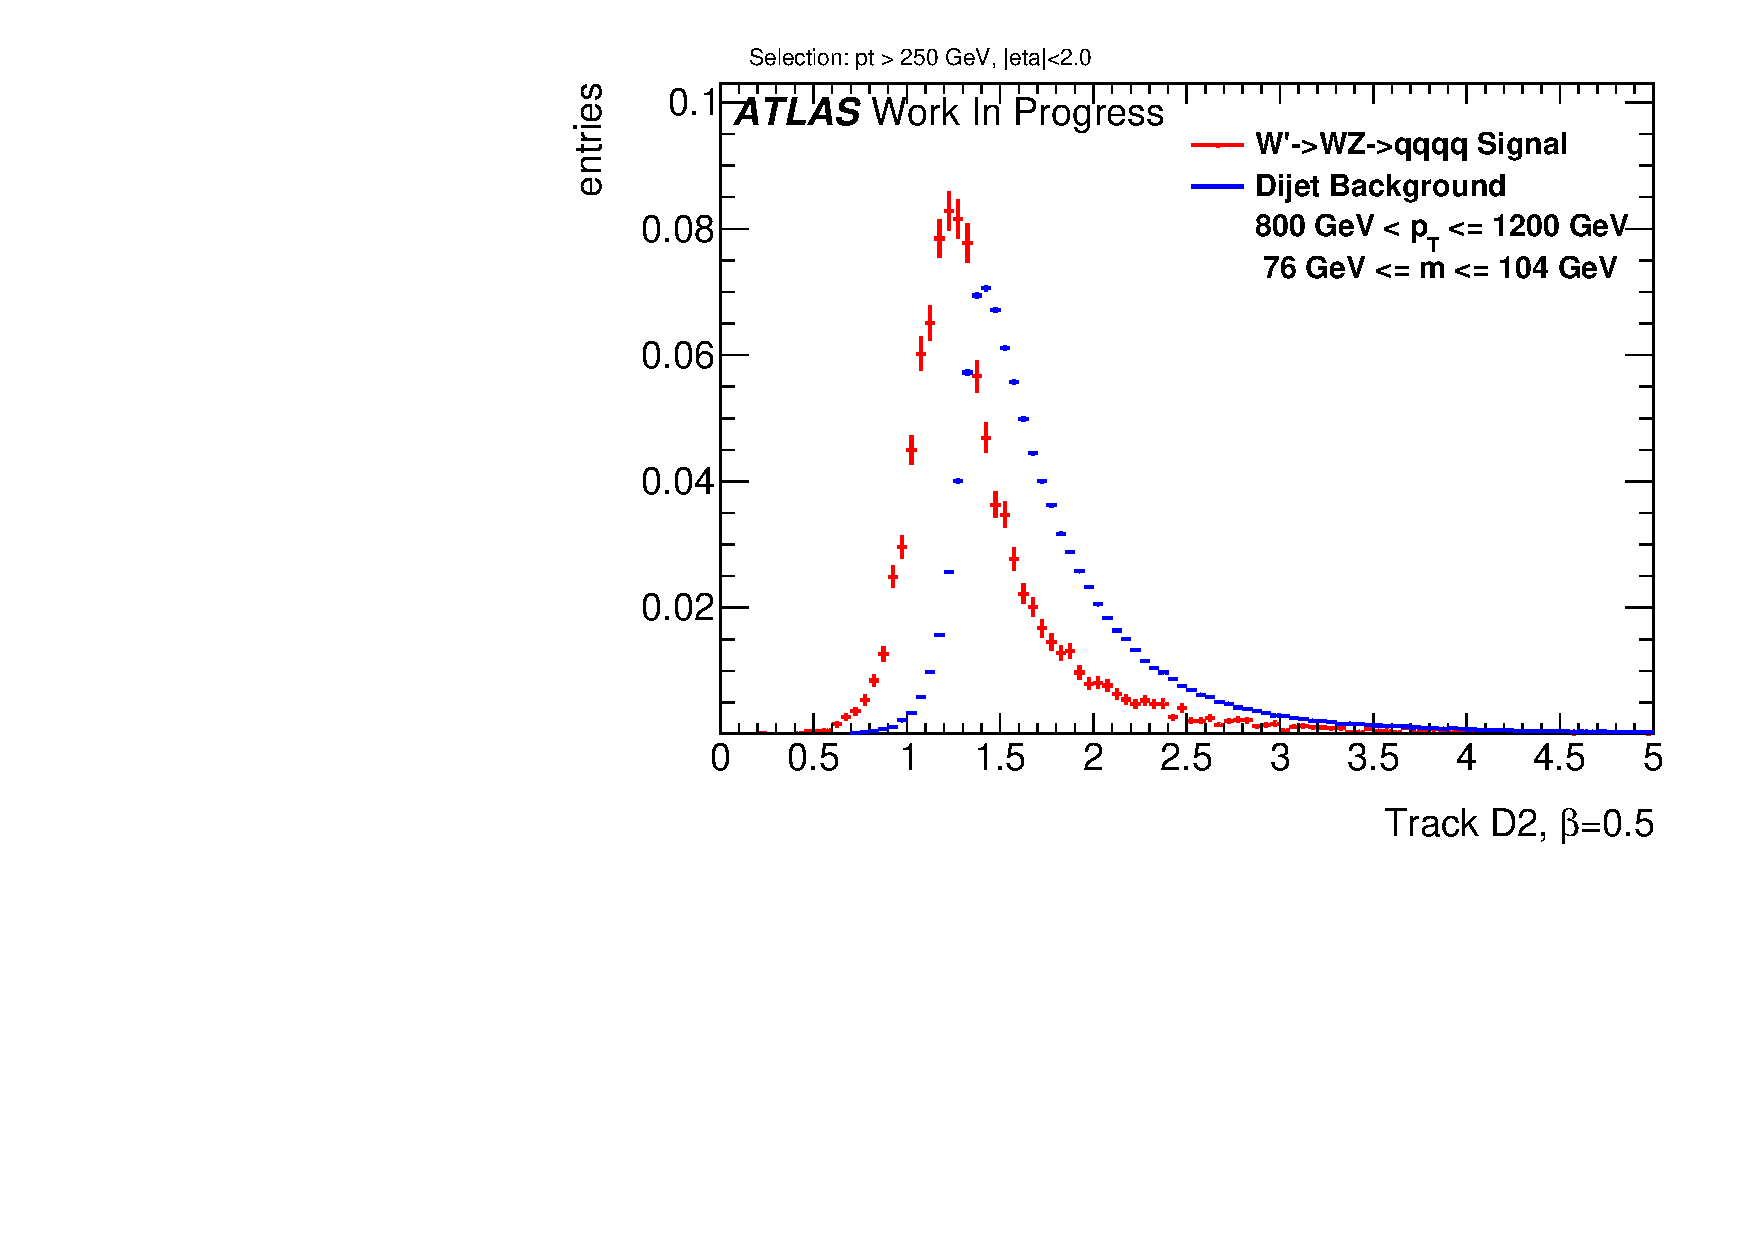
\includegraphics[width=0.3\textwidth]{sascha_input/Appendix/Distributions/w/distributions/beta05/h_normal_tj_D2_05_bin3.pdf} 
\bigskip
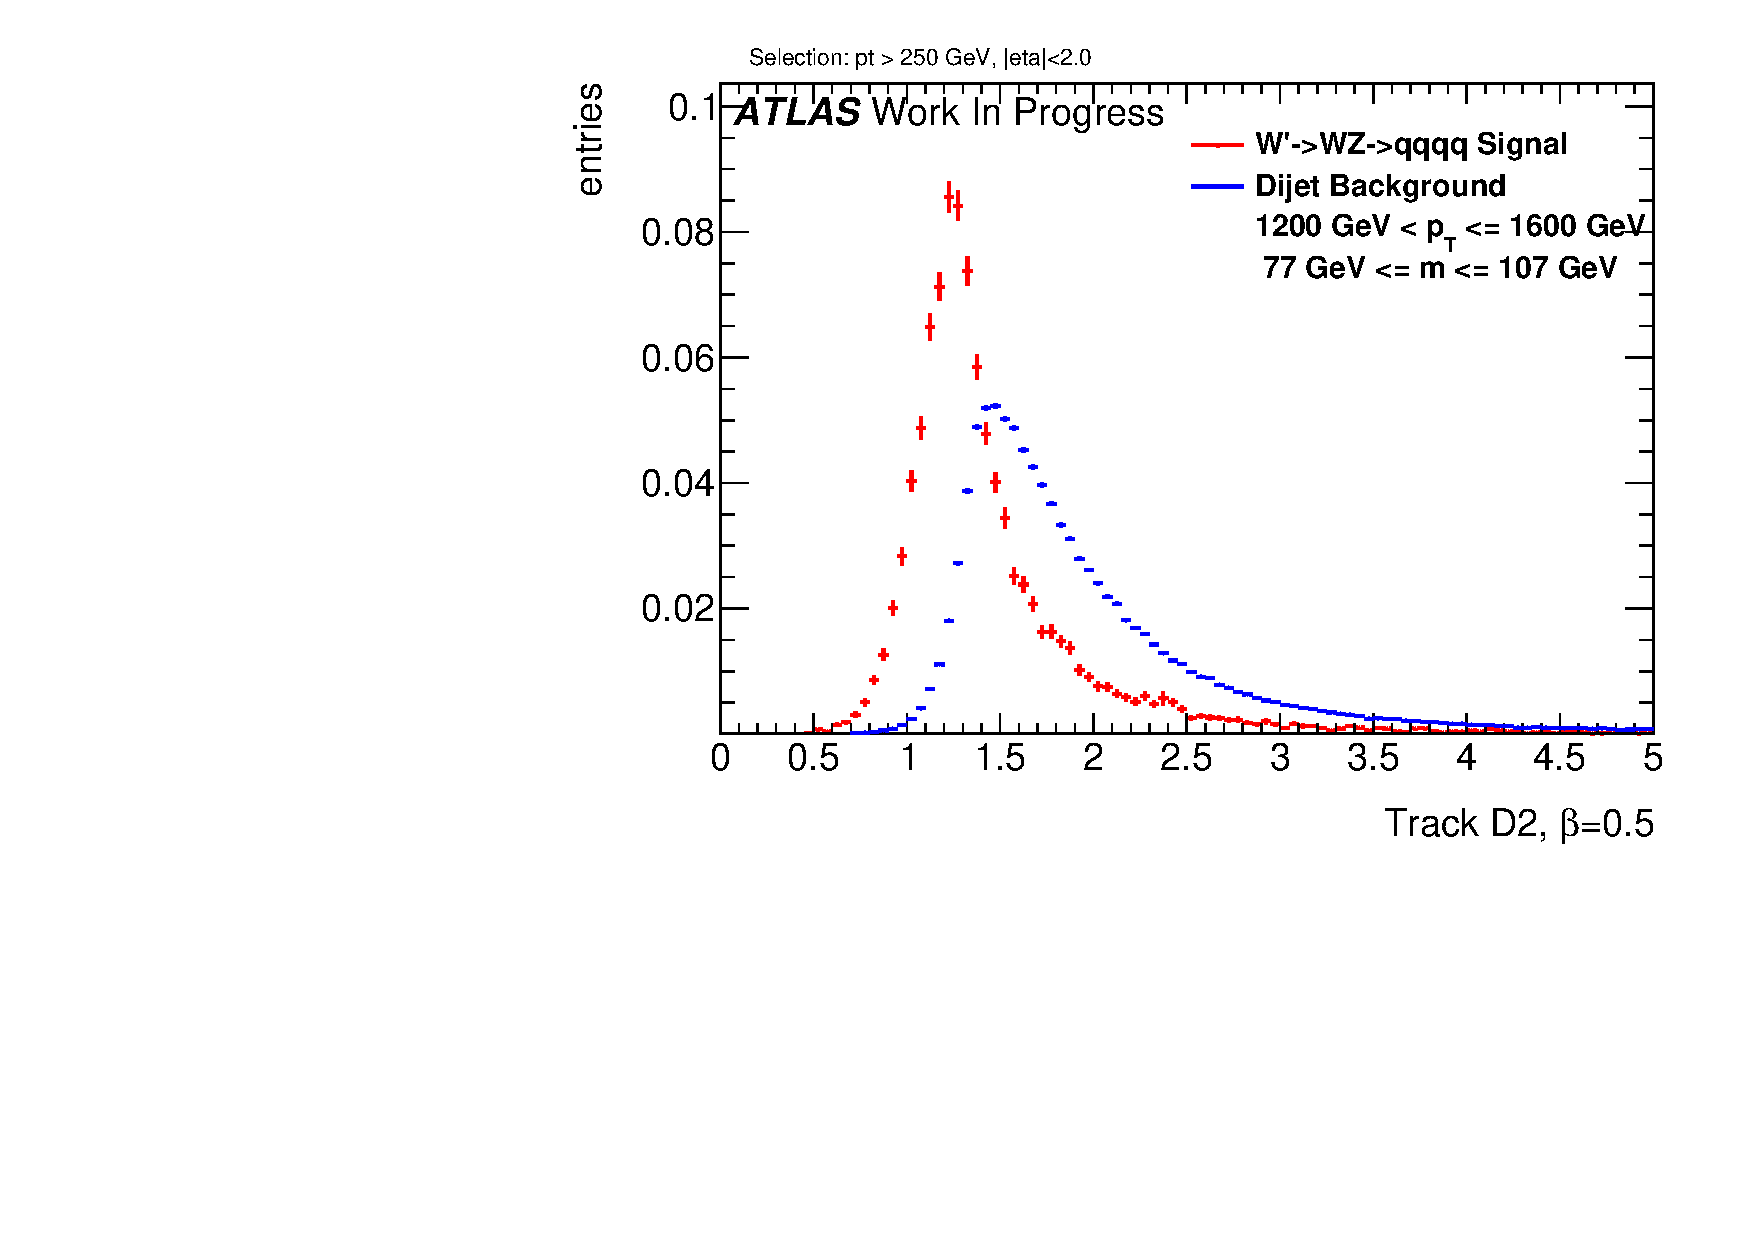
\includegraphics[width=0.3\textwidth]{sascha_input/Appendix/Distributions/w/distributions/beta05/h_normal_tj_D2_05_bin4.pdf} \hspace{1mm}
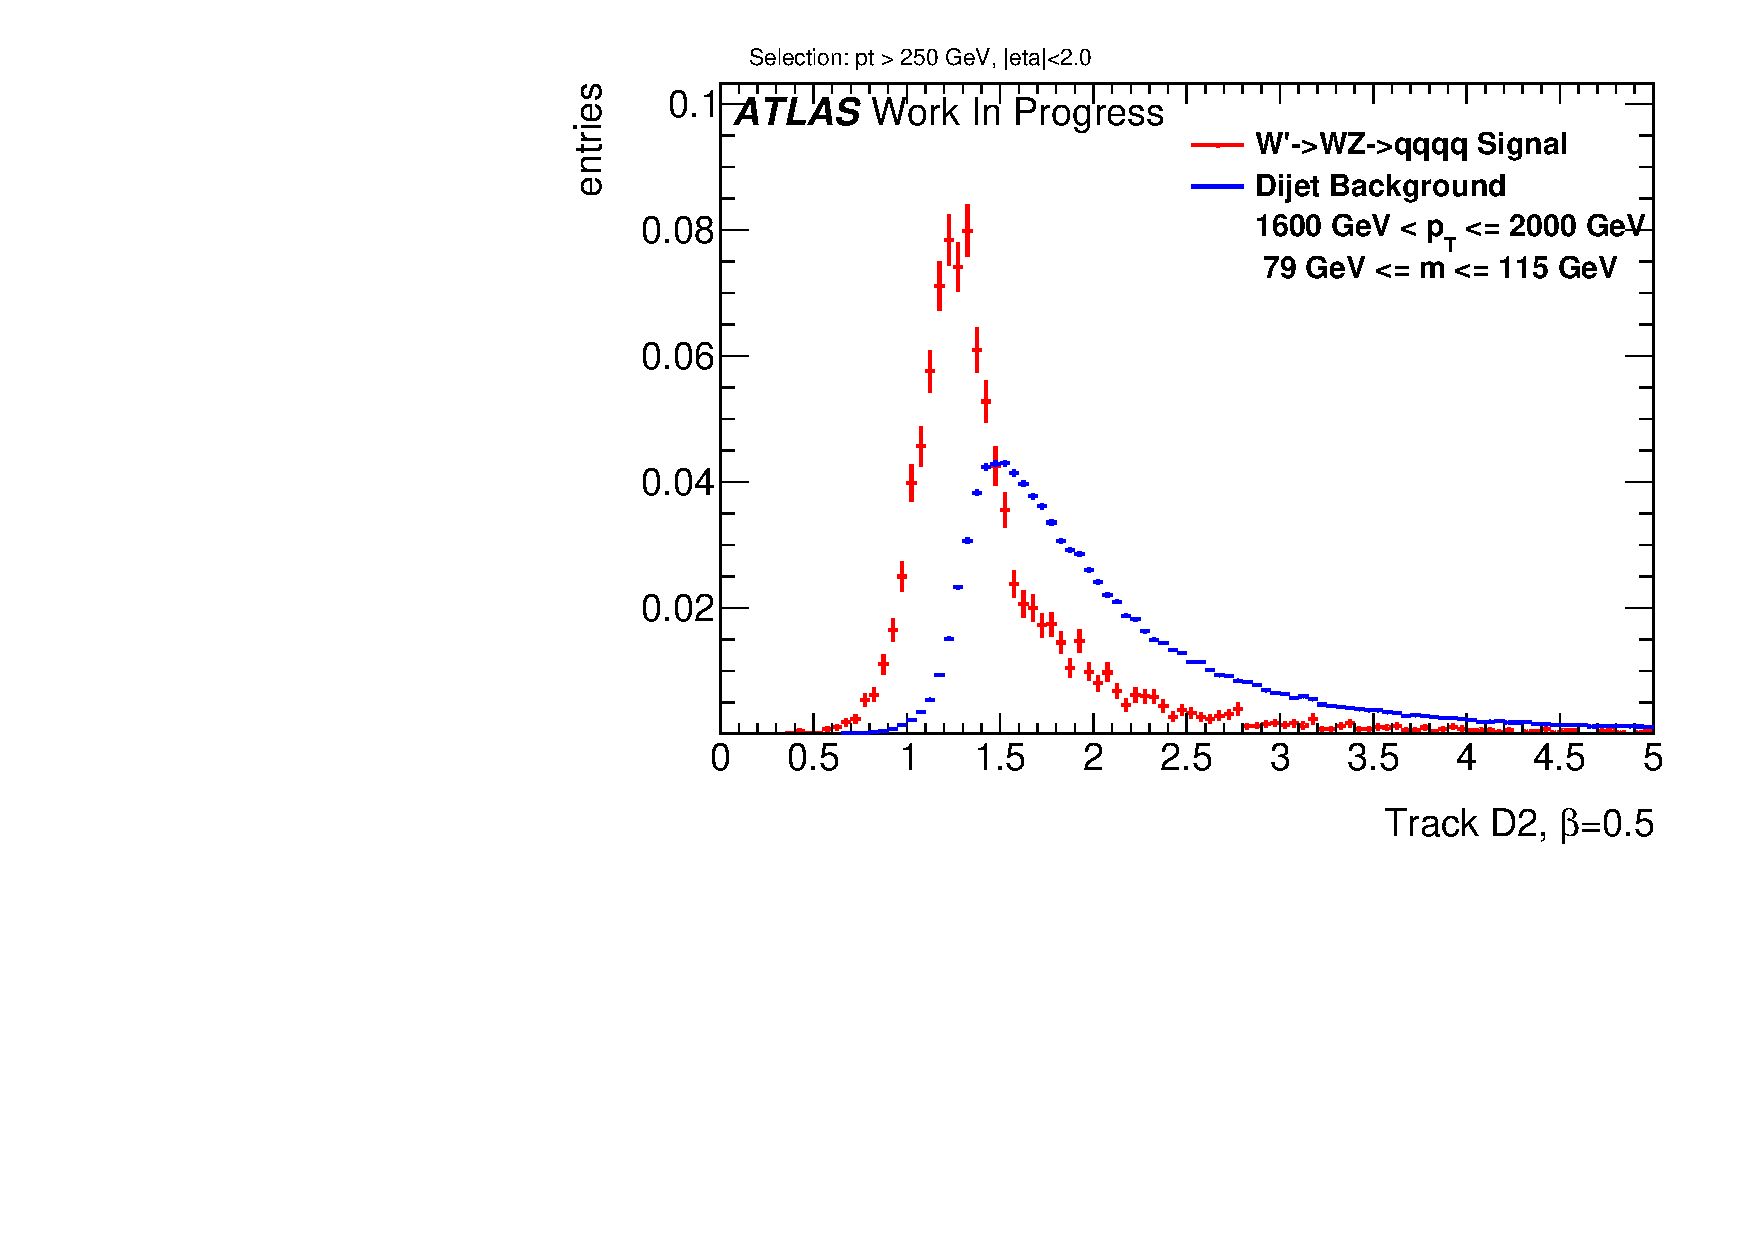
\includegraphics[width=0.3\textwidth]{sascha_input/Appendix/Distributions/w/distributions/beta05/h_normal_tj_D2_05_bin5.pdf} \hspace{1mm}
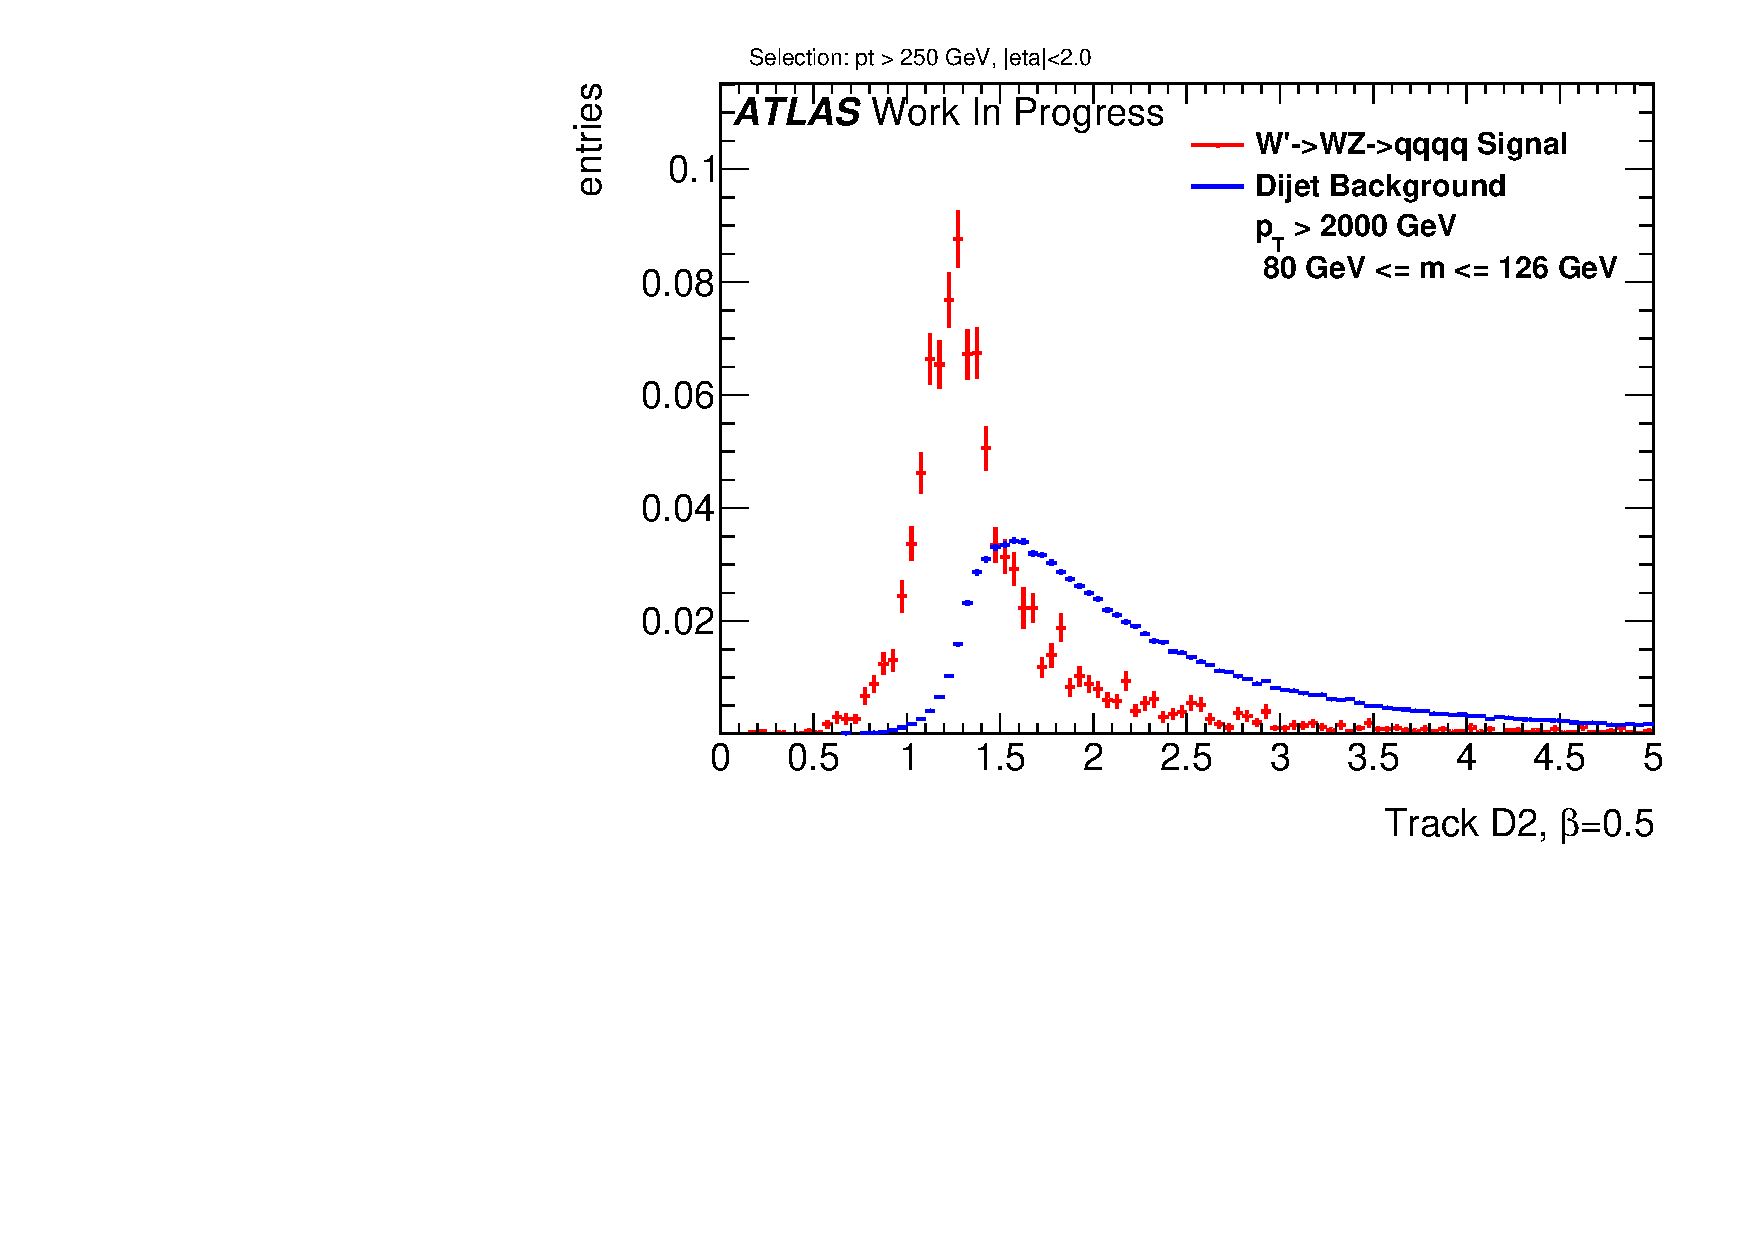
\includegraphics[width=0.3\textwidth]{sascha_input/Appendix/Distributions/w/distributions/beta05/h_normal_tj_D2_05_bin6.pdf}
\bigskip
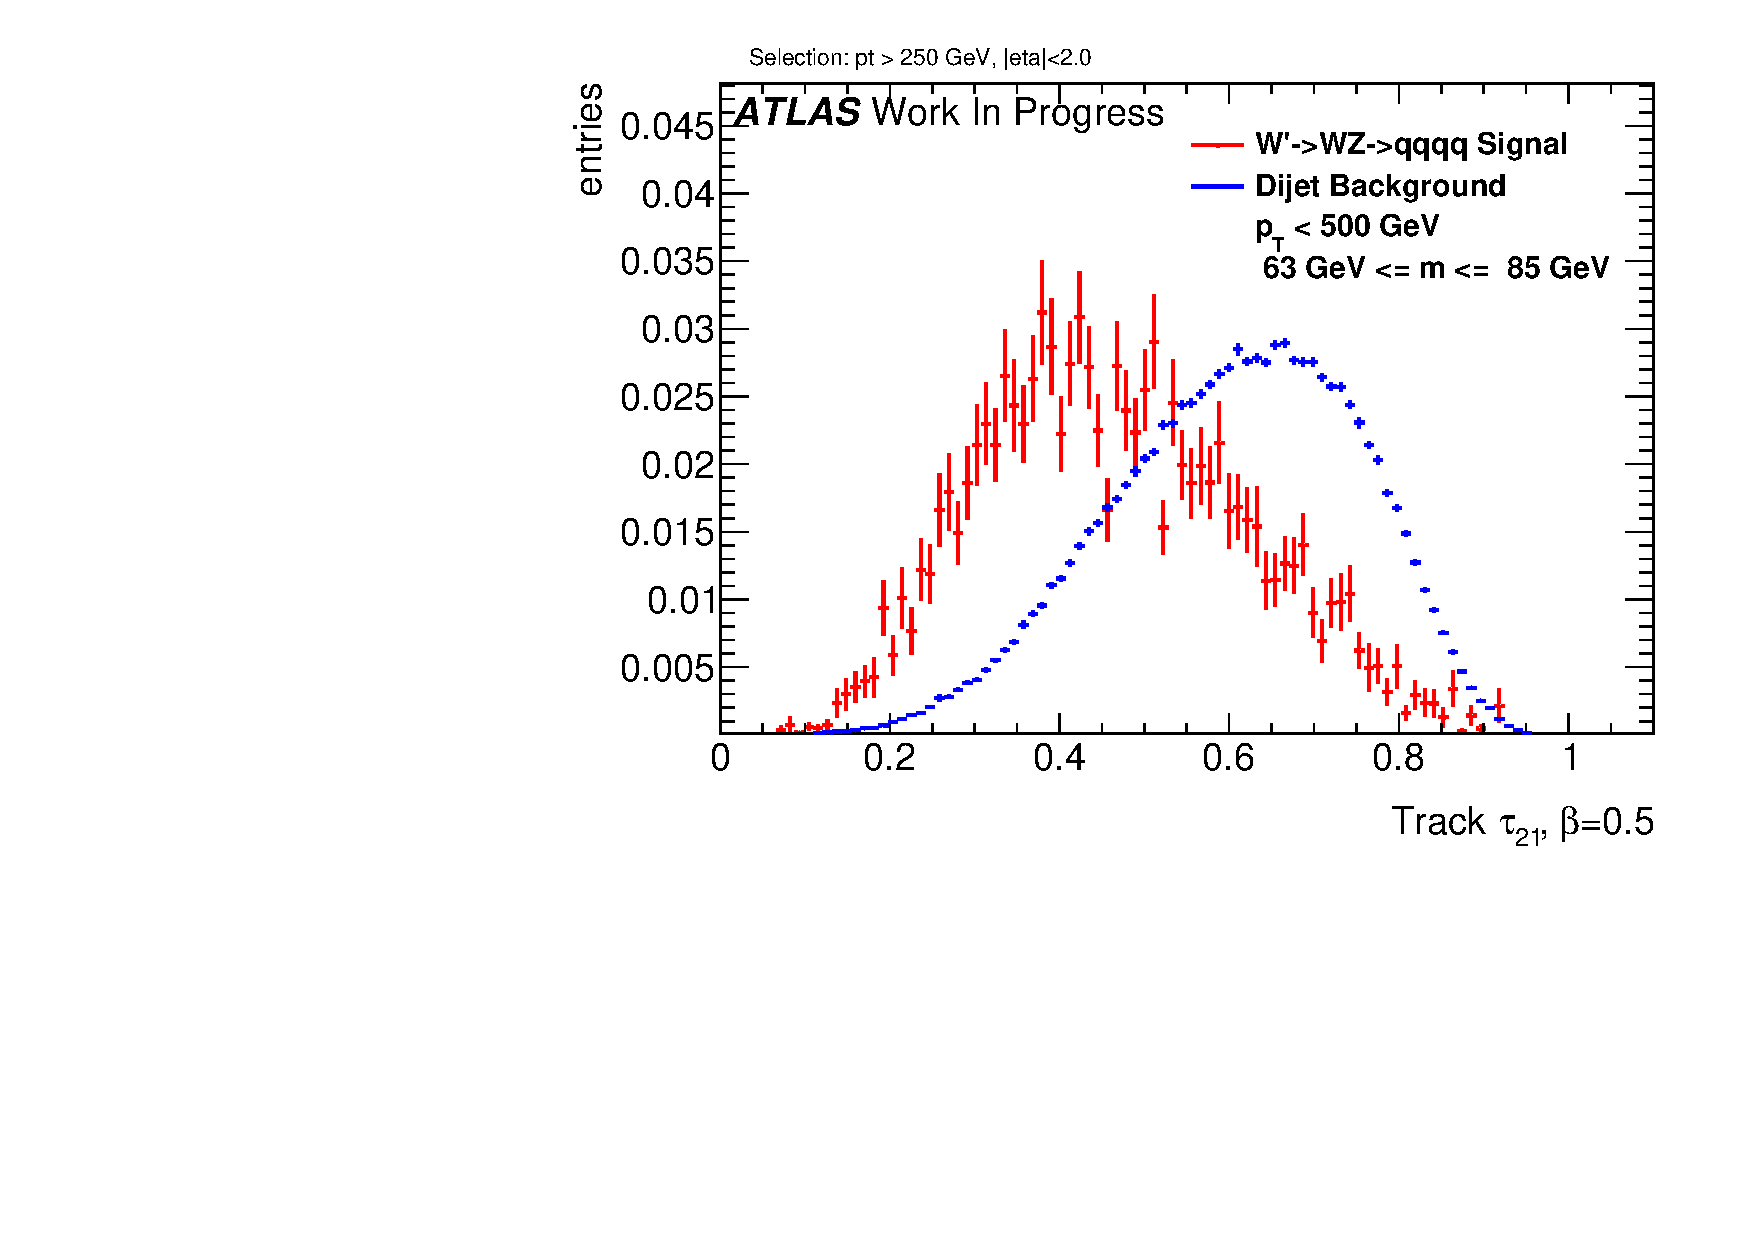
\includegraphics[width=0.3\textwidth]{sascha_input/Appendix/Distributions/w/distributions/beta05/h_normal_tj_nSub21_05_bin1.pdf} \hspace{1mm}
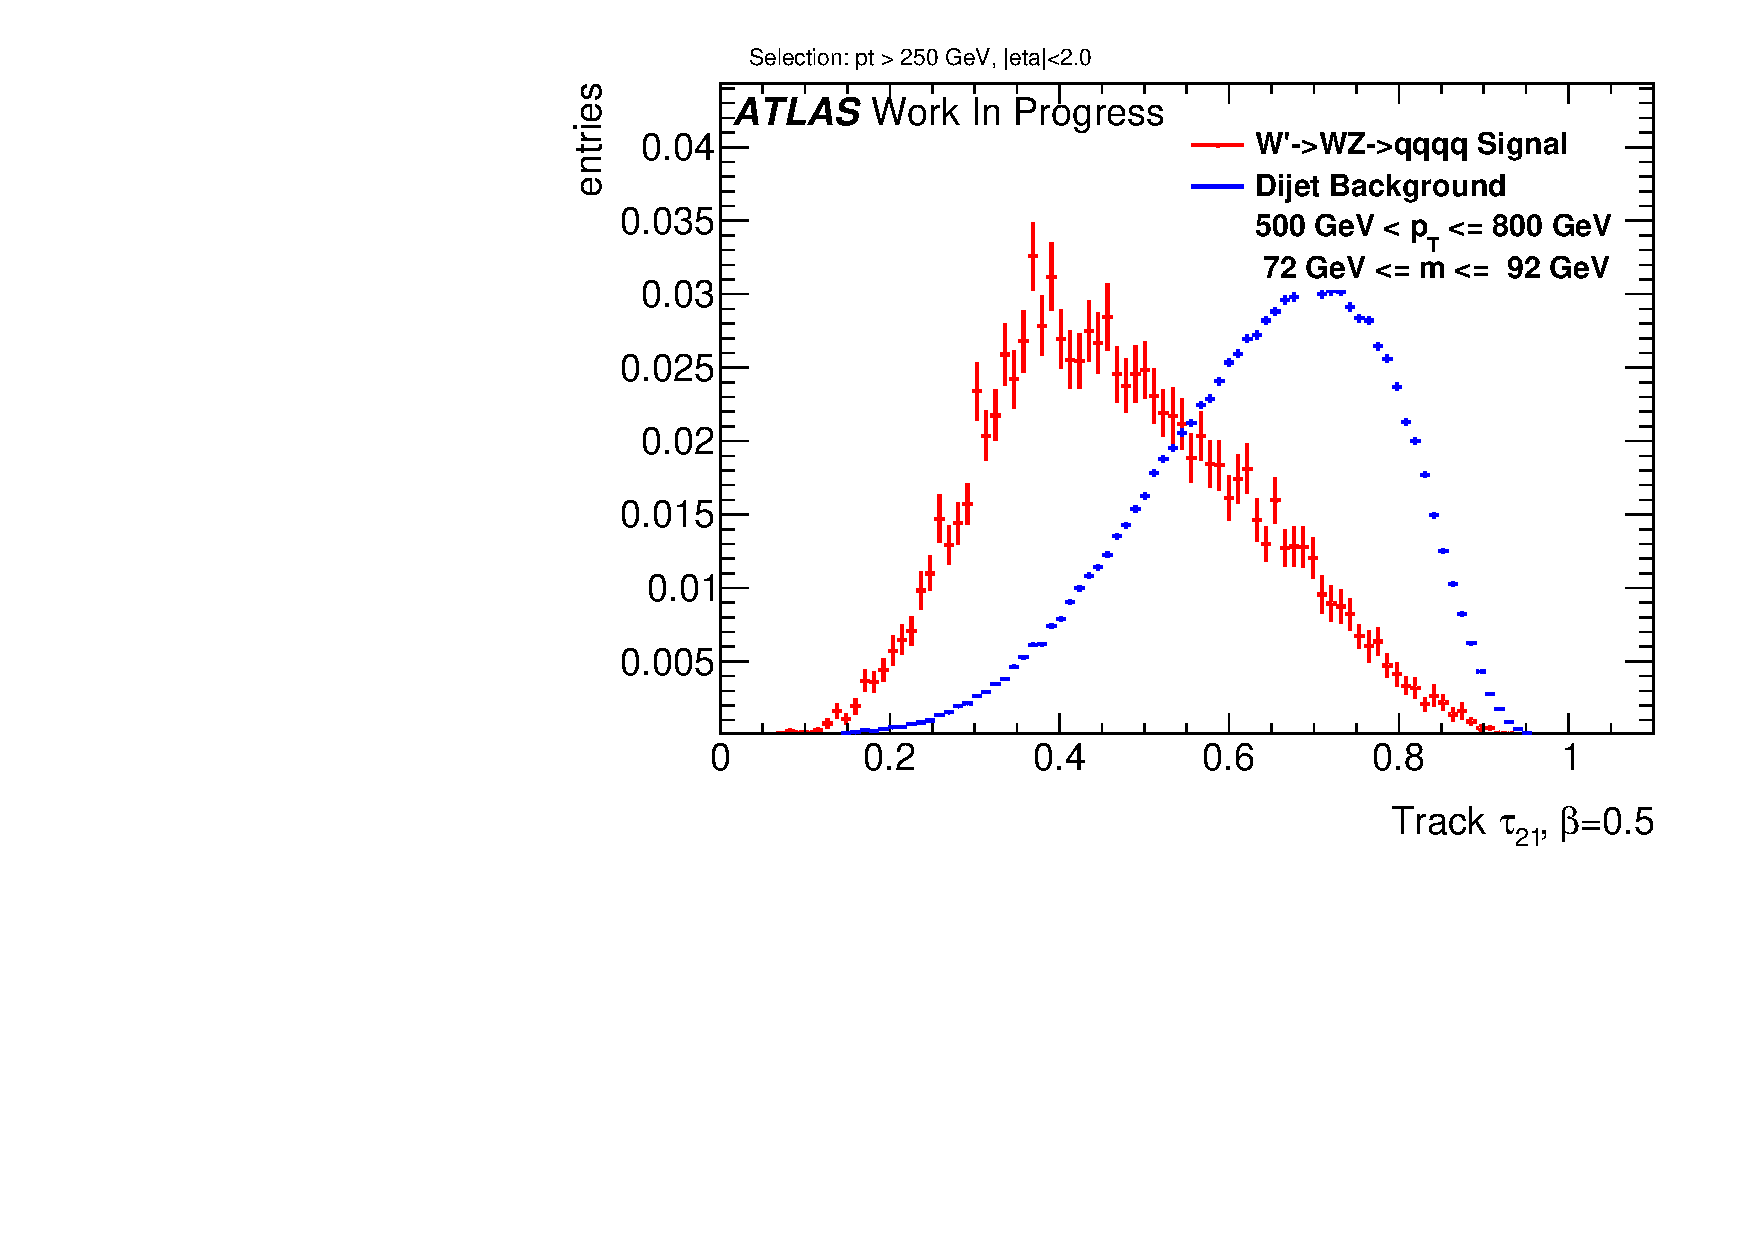
\includegraphics[width=0.3\textwidth]{sascha_input/Appendix/Distributions/w/distributions/beta05/h_normal_tj_nSub21_05_bin2.pdf} \hspace{1mm}
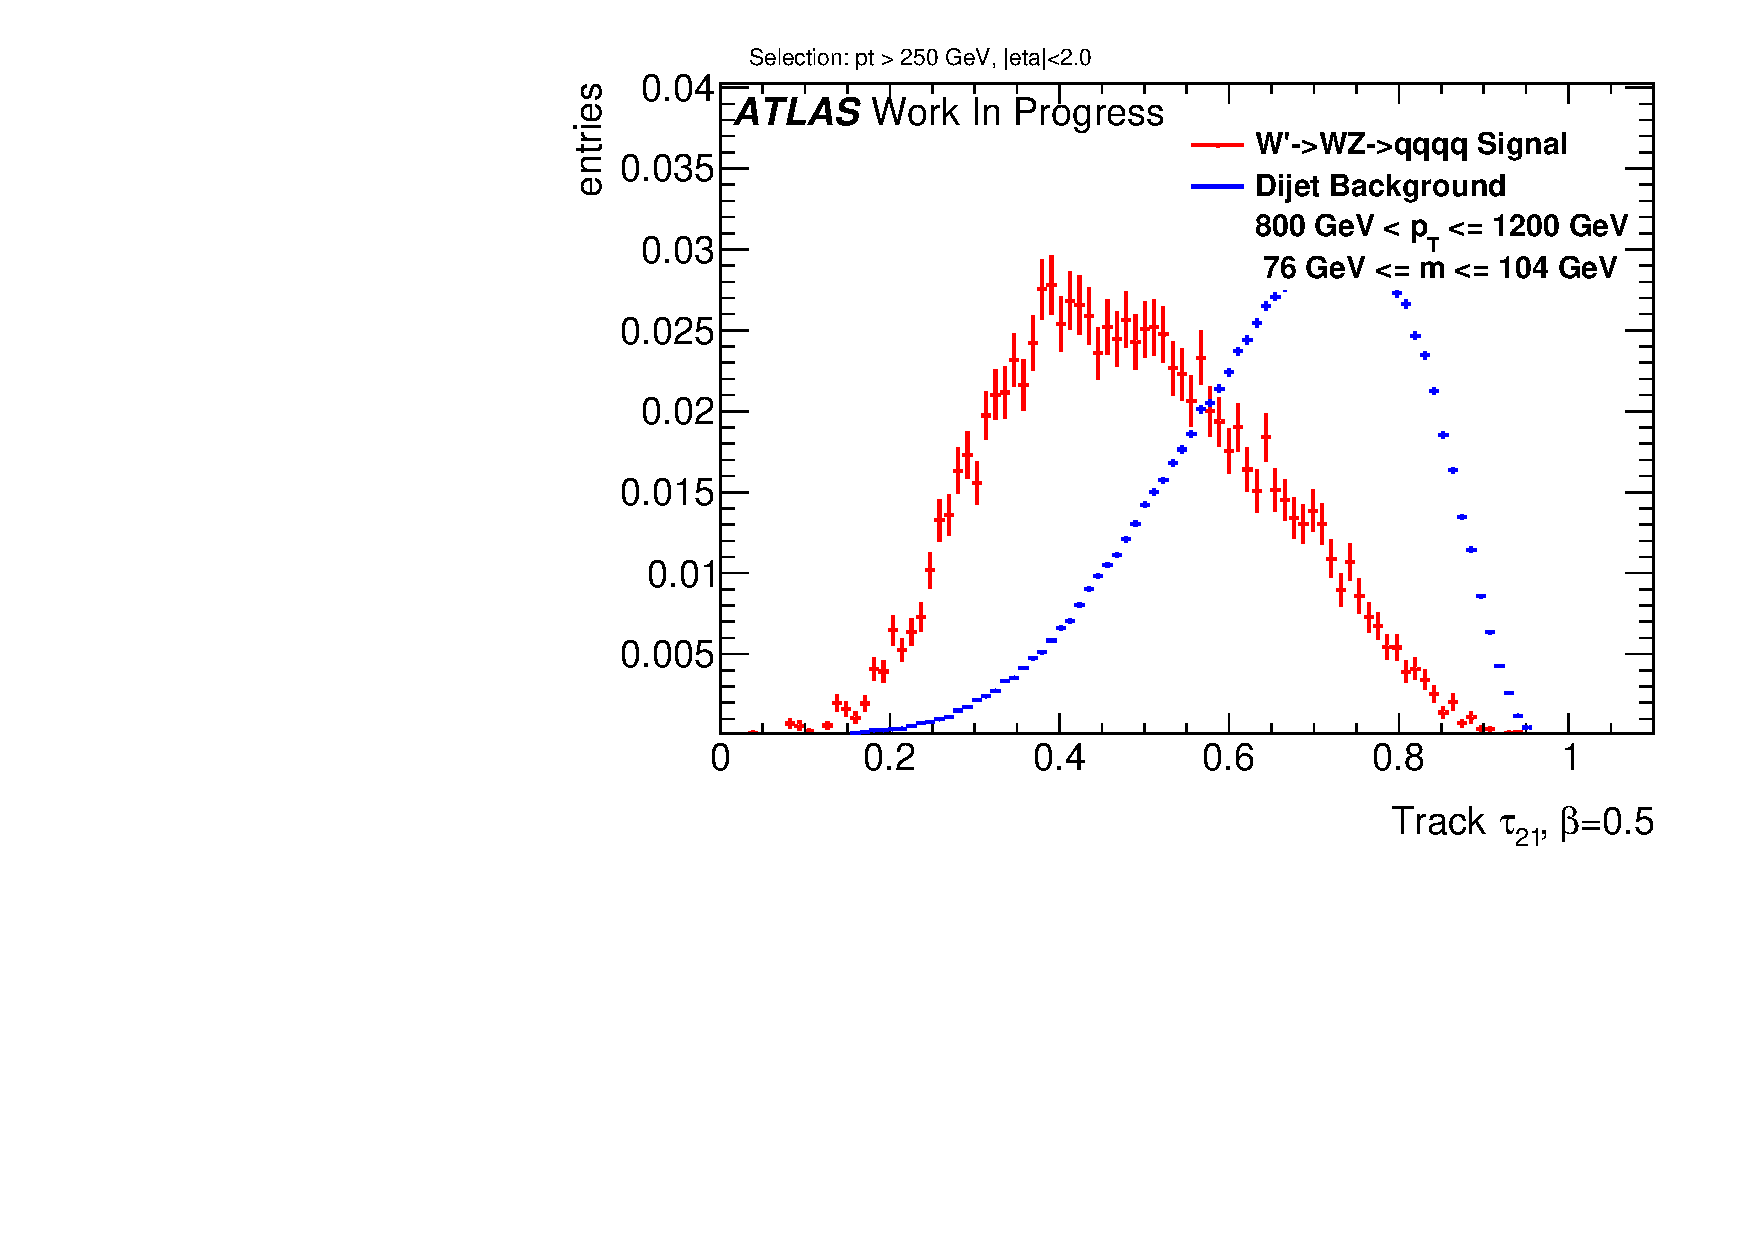
\includegraphics[width=0.3\textwidth]{sascha_input/Appendix/Distributions/w/distributions/beta05/h_normal_tj_nSub21_05_bin3.pdf} 
\bigskip
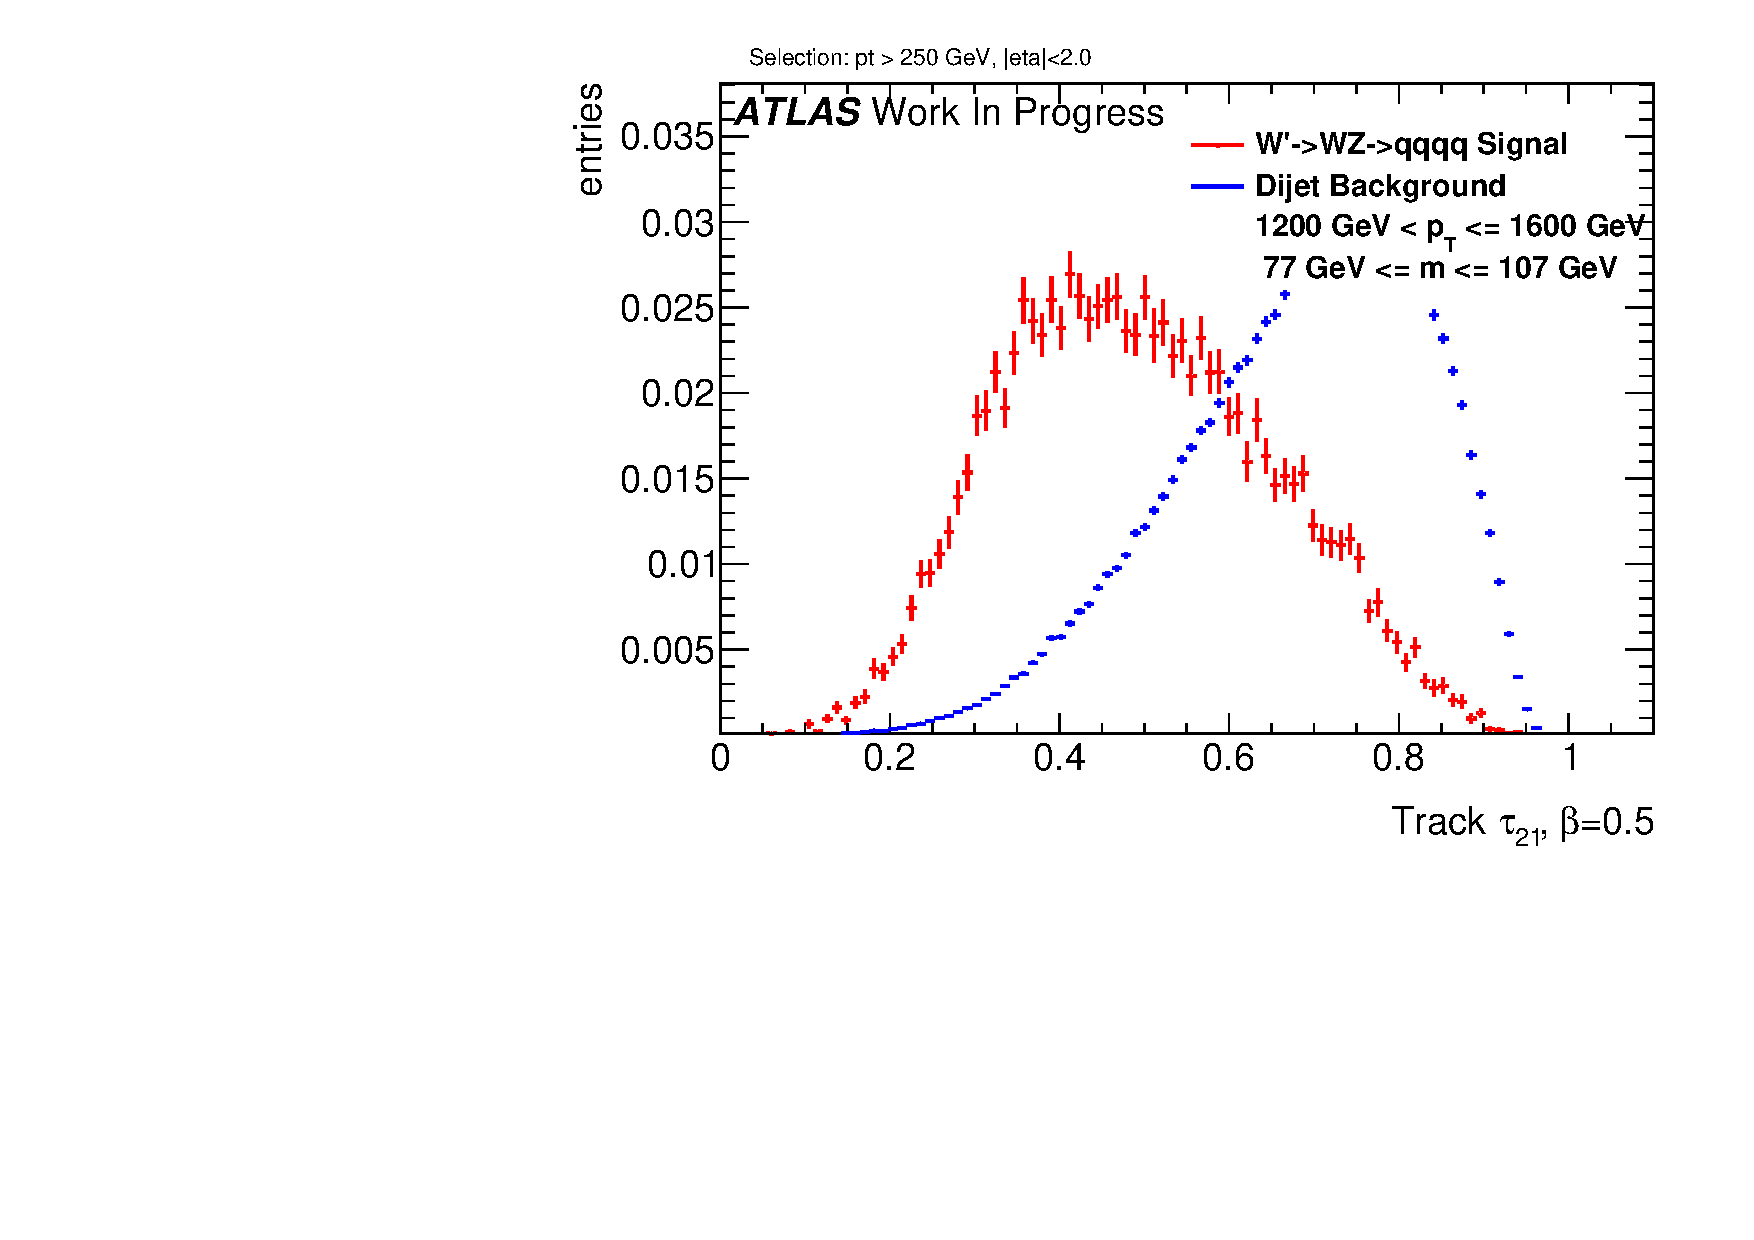
\includegraphics[width=0.3\textwidth]{sascha_input/Appendix/Distributions/w/distributions/beta05/h_normal_tj_nSub21_05_bin4.pdf} \hspace{6mm}
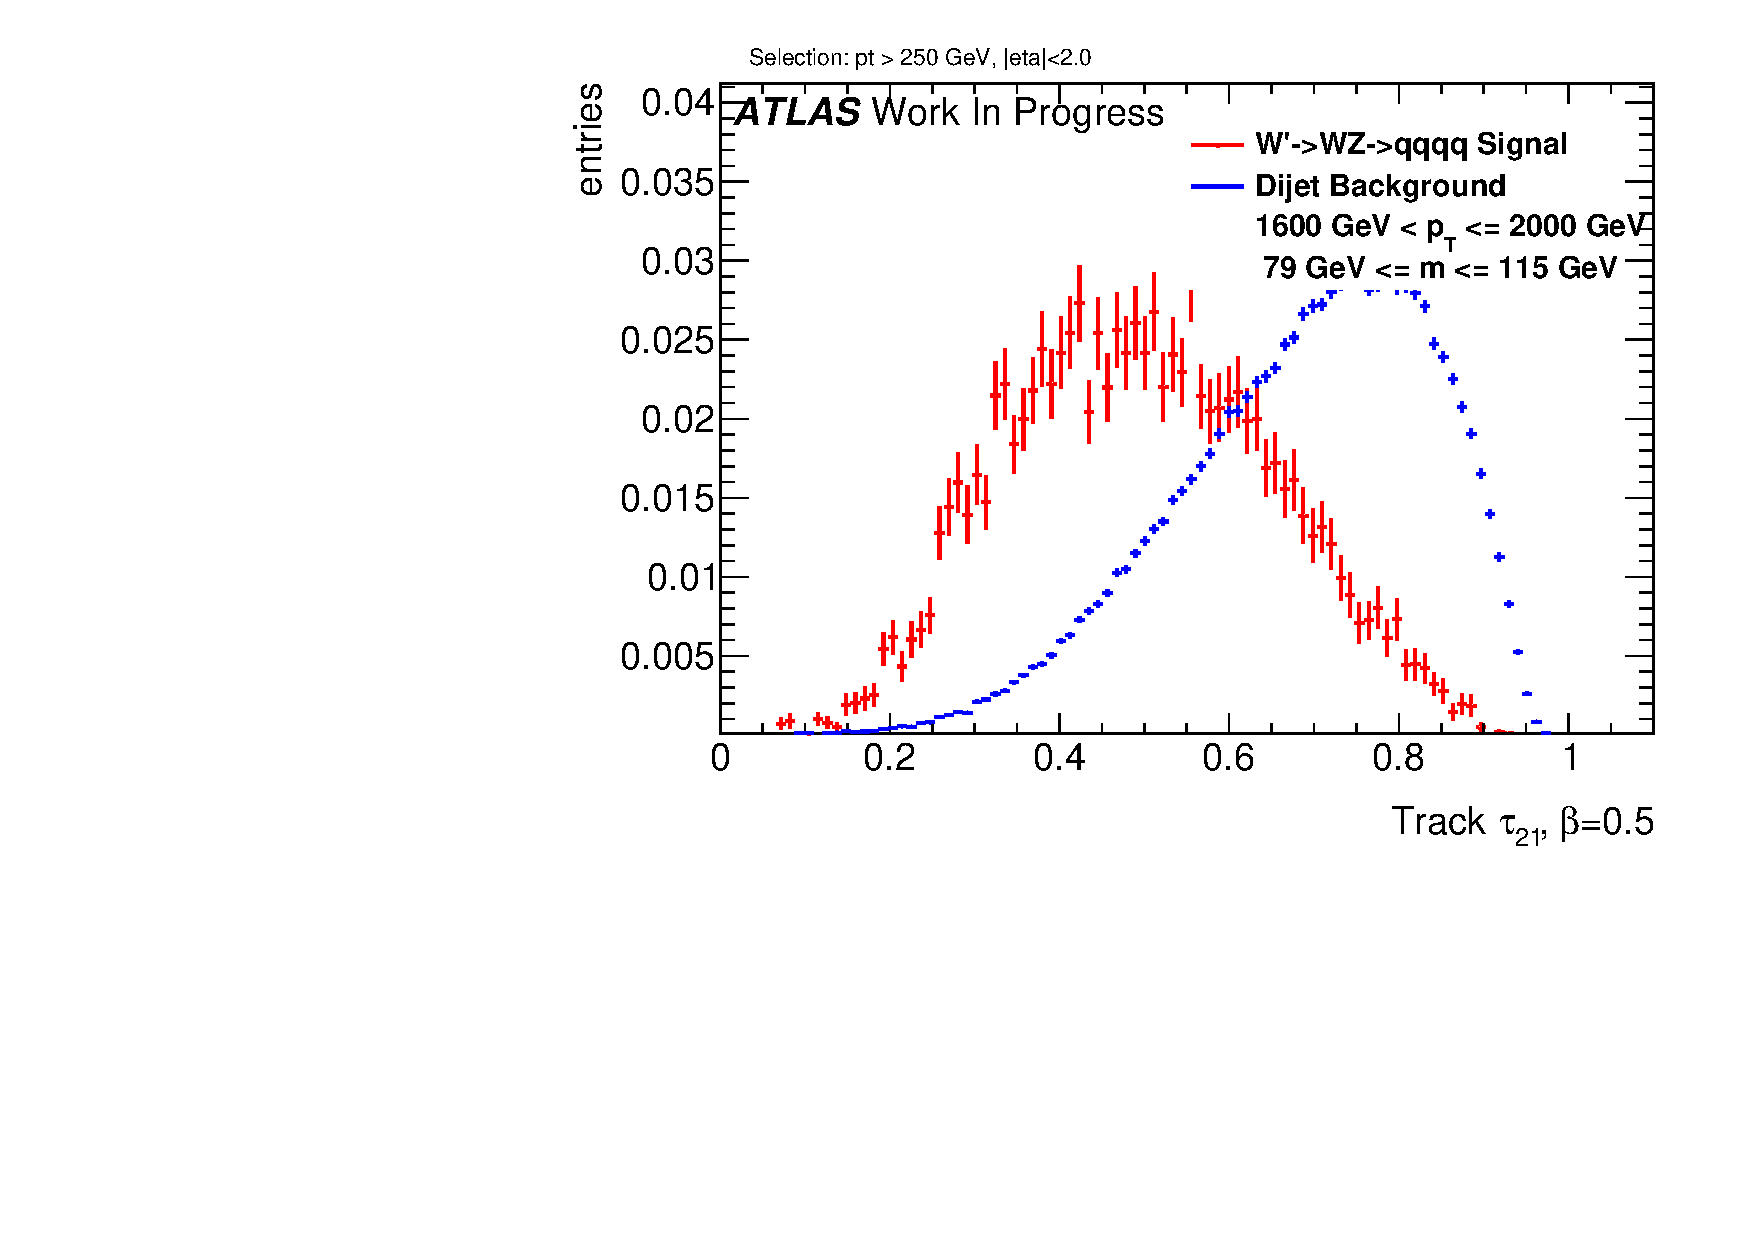
\includegraphics[width=0.3\textwidth]{sascha_input/Appendix/Distributions/w/distributions/beta05/h_normal_tj_nSub21_05_bin5.pdf} \hspace{6mm}
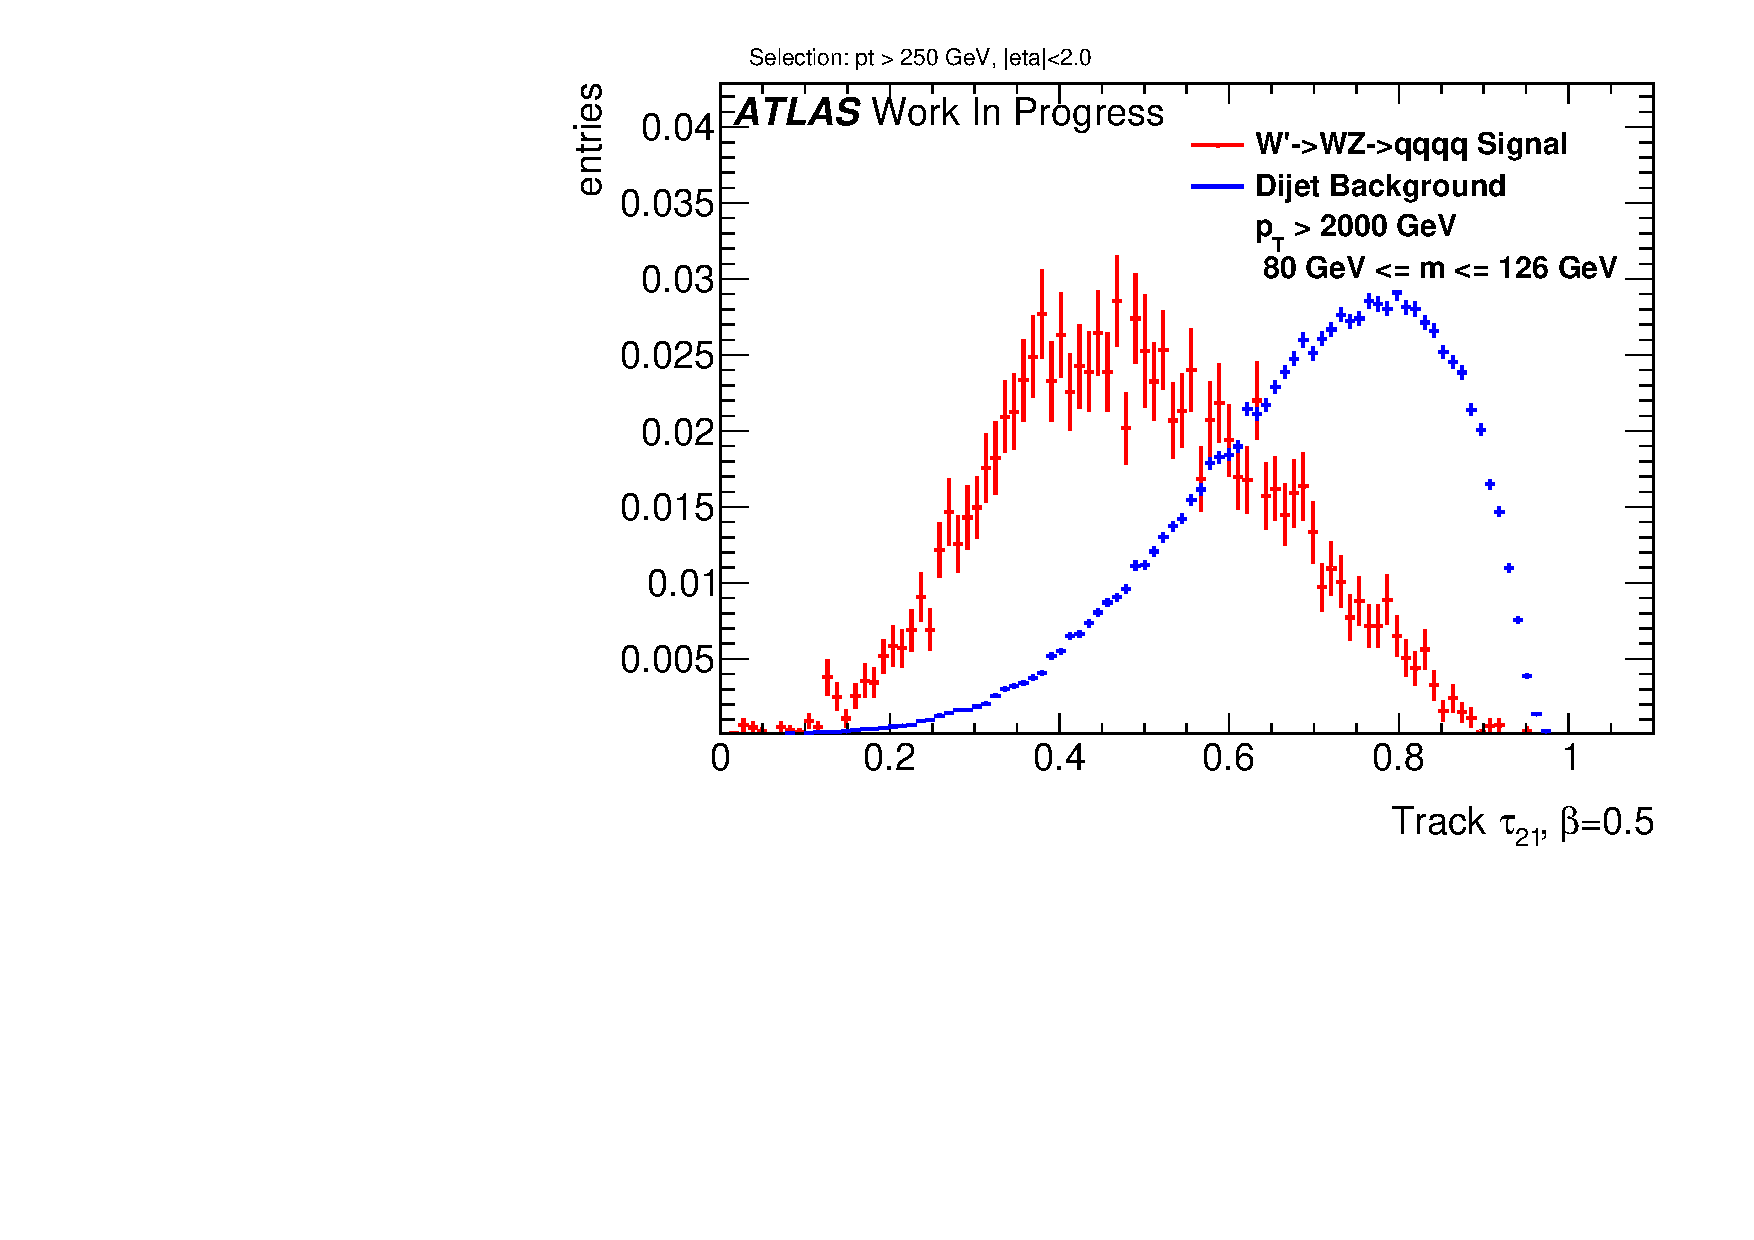
\includegraphics[width=0.3\textwidth]{sascha_input/Appendix/Distributions/w/distributions/beta05/h_normal_tj_nSub21_05_bin6.pdf}
\caption{{Distributions for $W$ boson tagging using tracks $\beta=0.5$. C2, D2, $\tau_{21}$ top down.}}
\end{figure}
\begin{figure}[H]
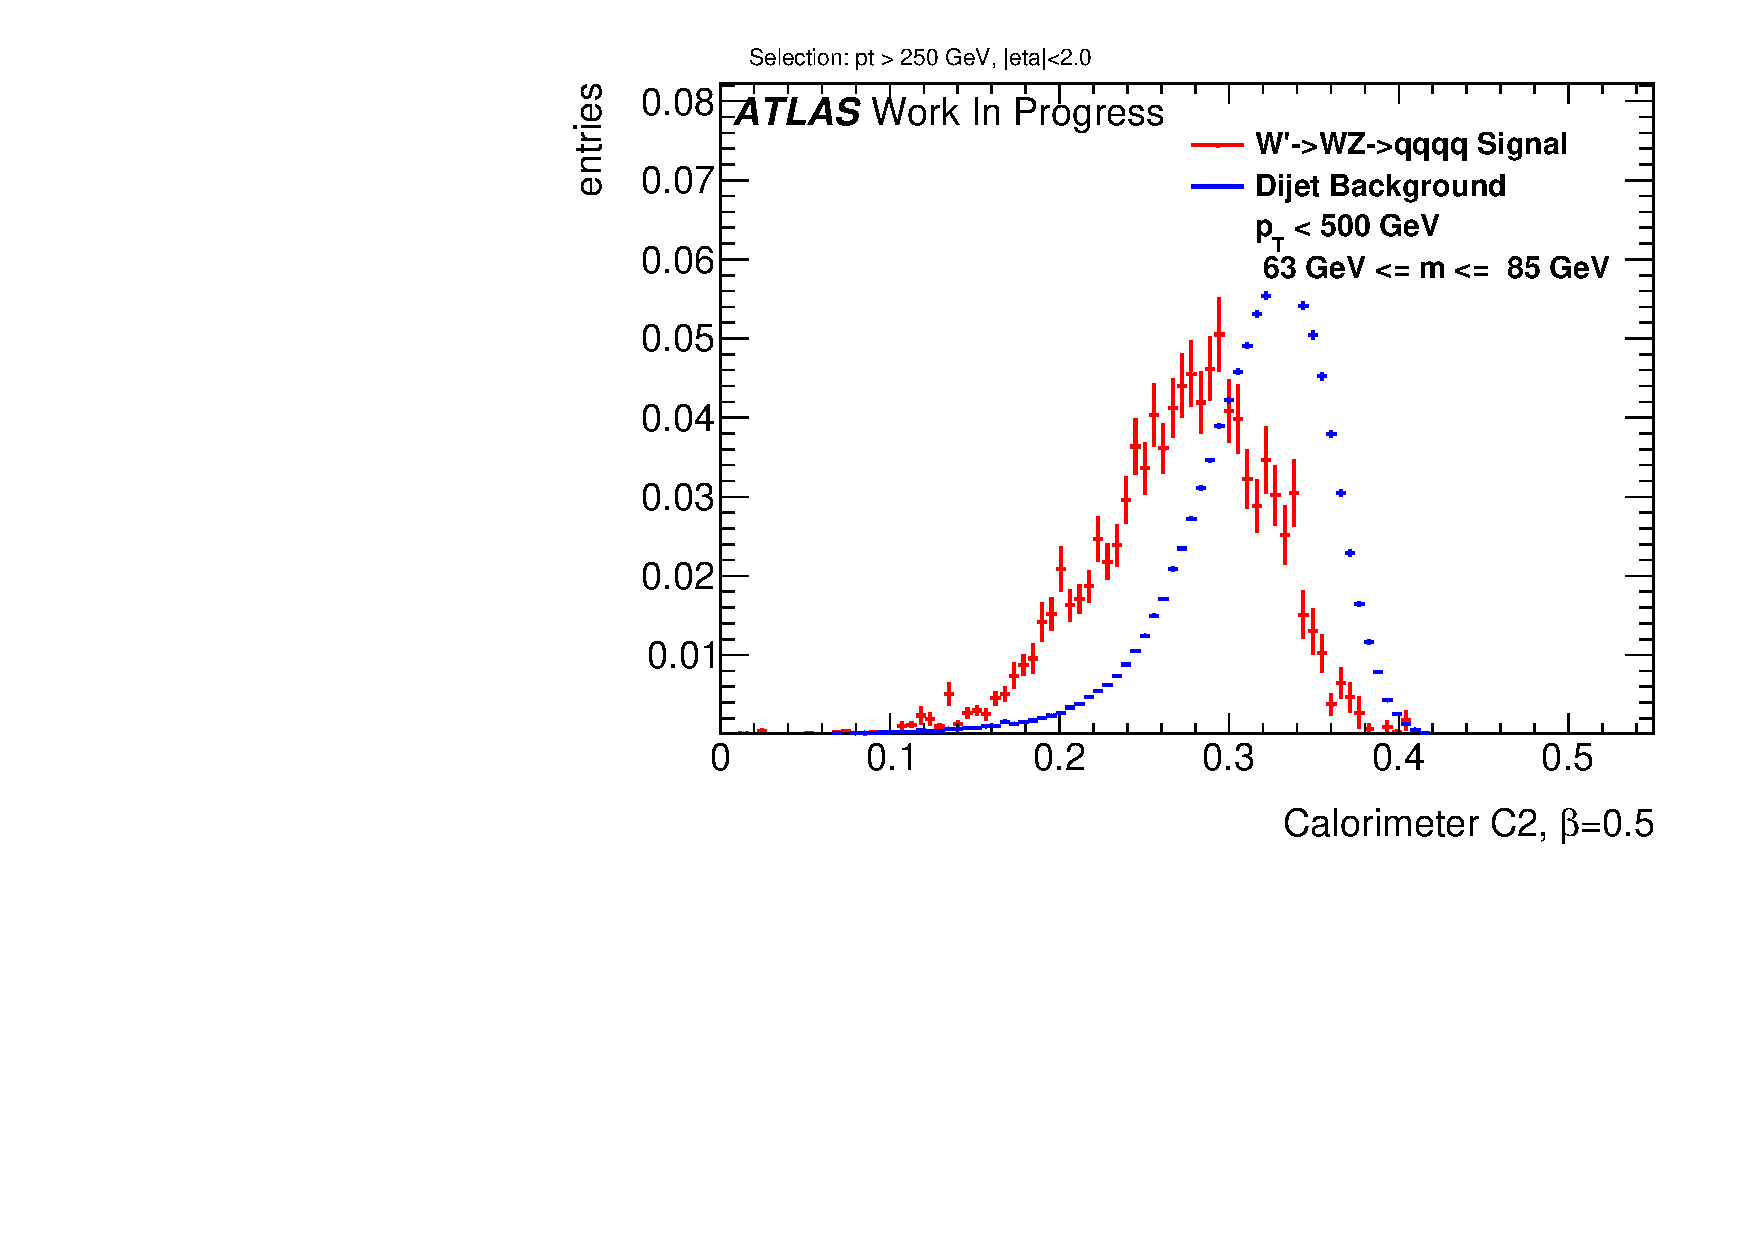
\includegraphics[width=0.3\textwidth]{sascha_input/Appendix/Distributions/w/distributions/beta05/h_recoJet_C2_05_bin1.pdf} \hspace{1mm}
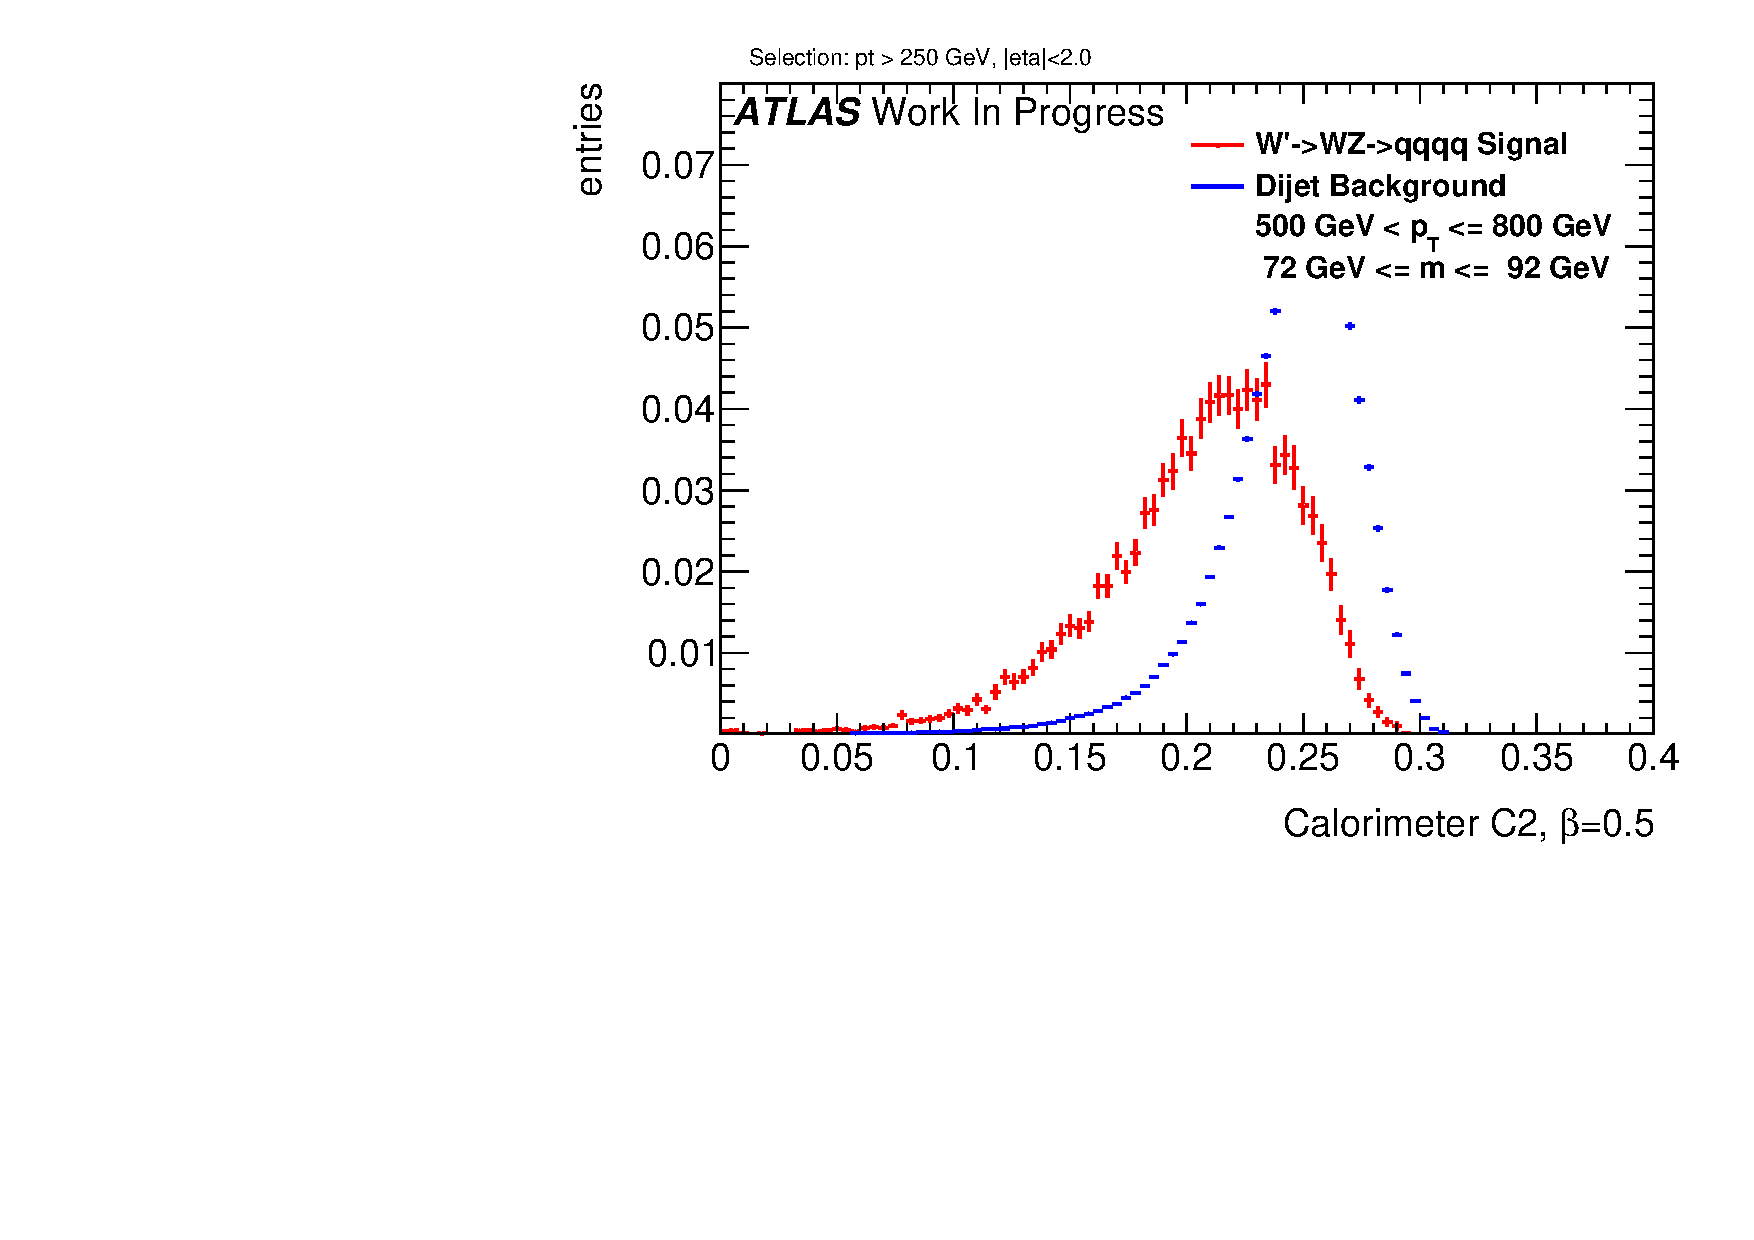
\includegraphics[width=0.3\textwidth]{sascha_input/Appendix/Distributions/w/distributions/beta05/h_recoJet_C2_05_bin2.pdf} \hspace{1mm}
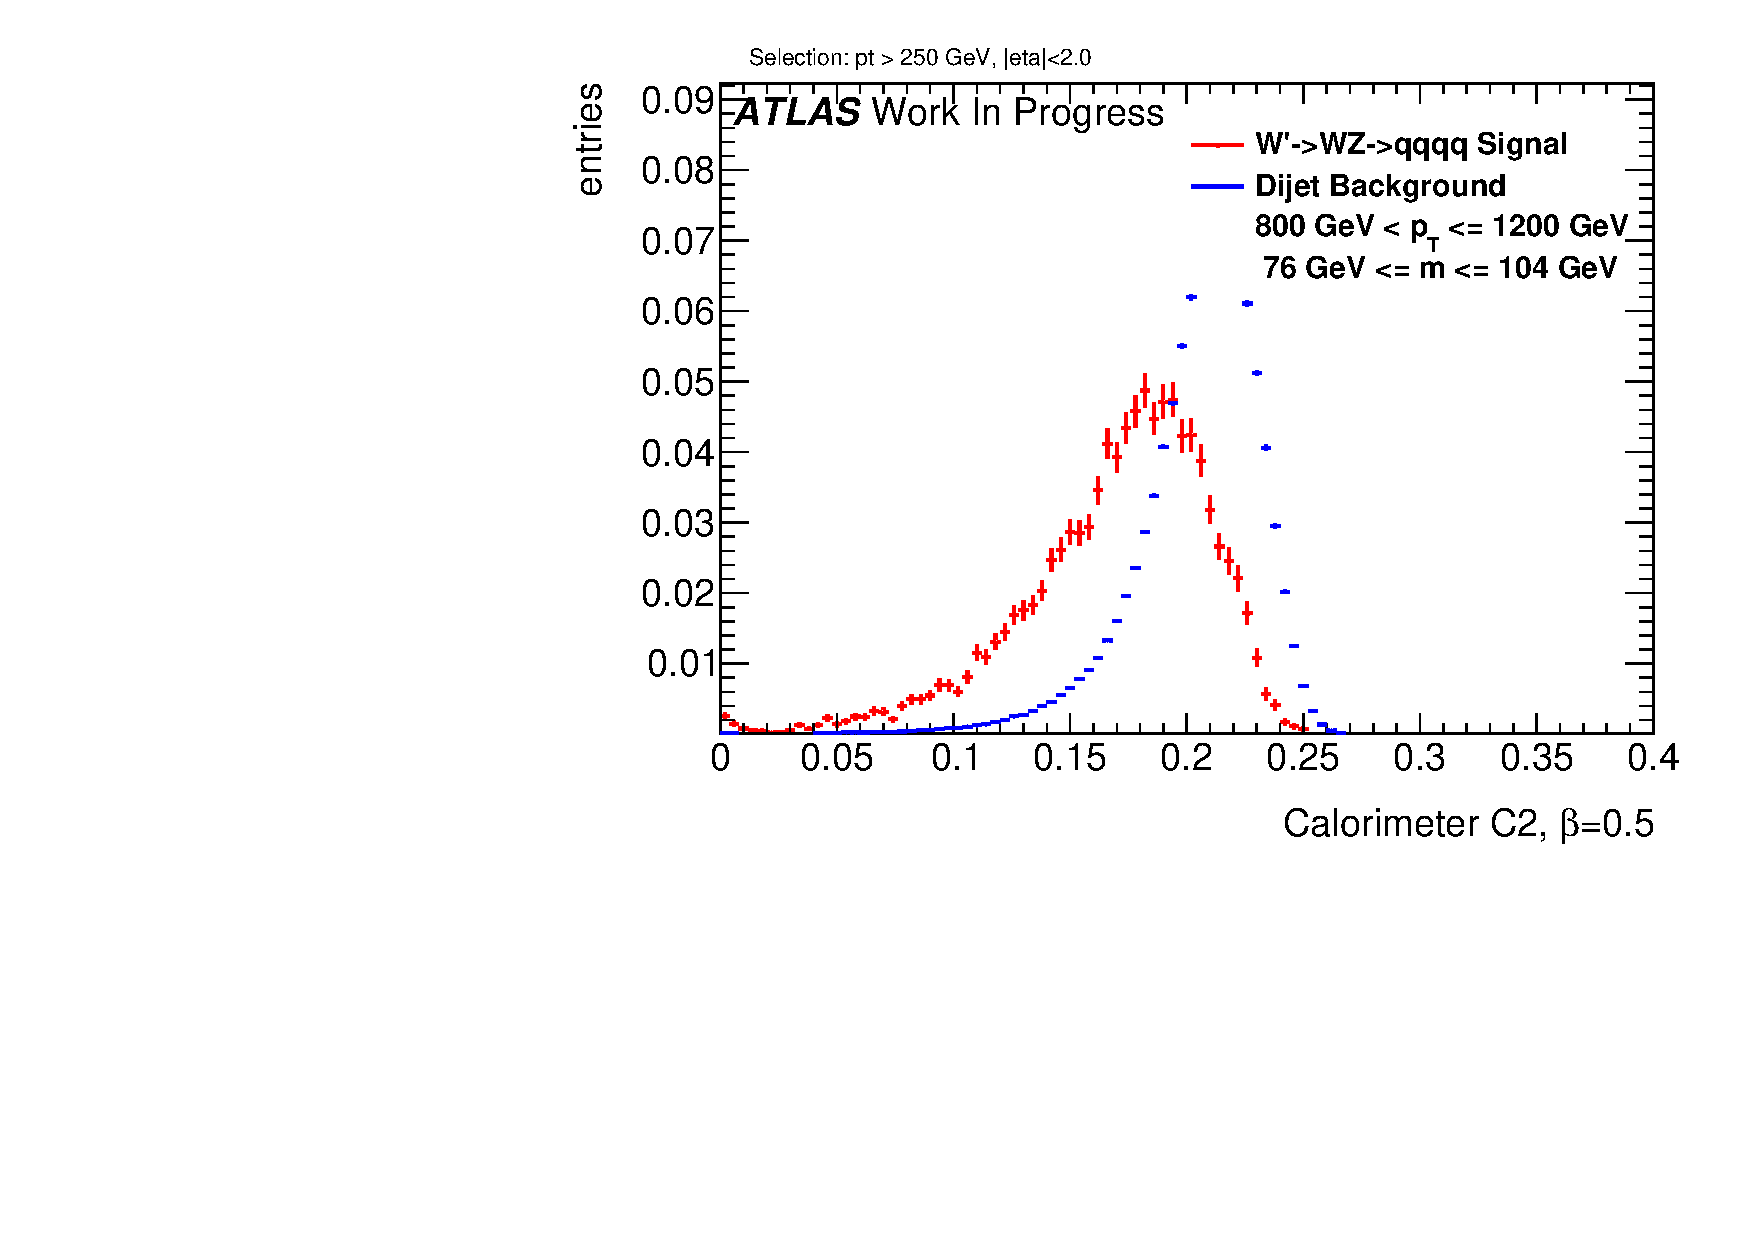
\includegraphics[width=0.3\textwidth]{sascha_input/Appendix/Distributions/w/distributions/beta05/h_recoJet_C2_05_bin3.pdf} 
\bigskip
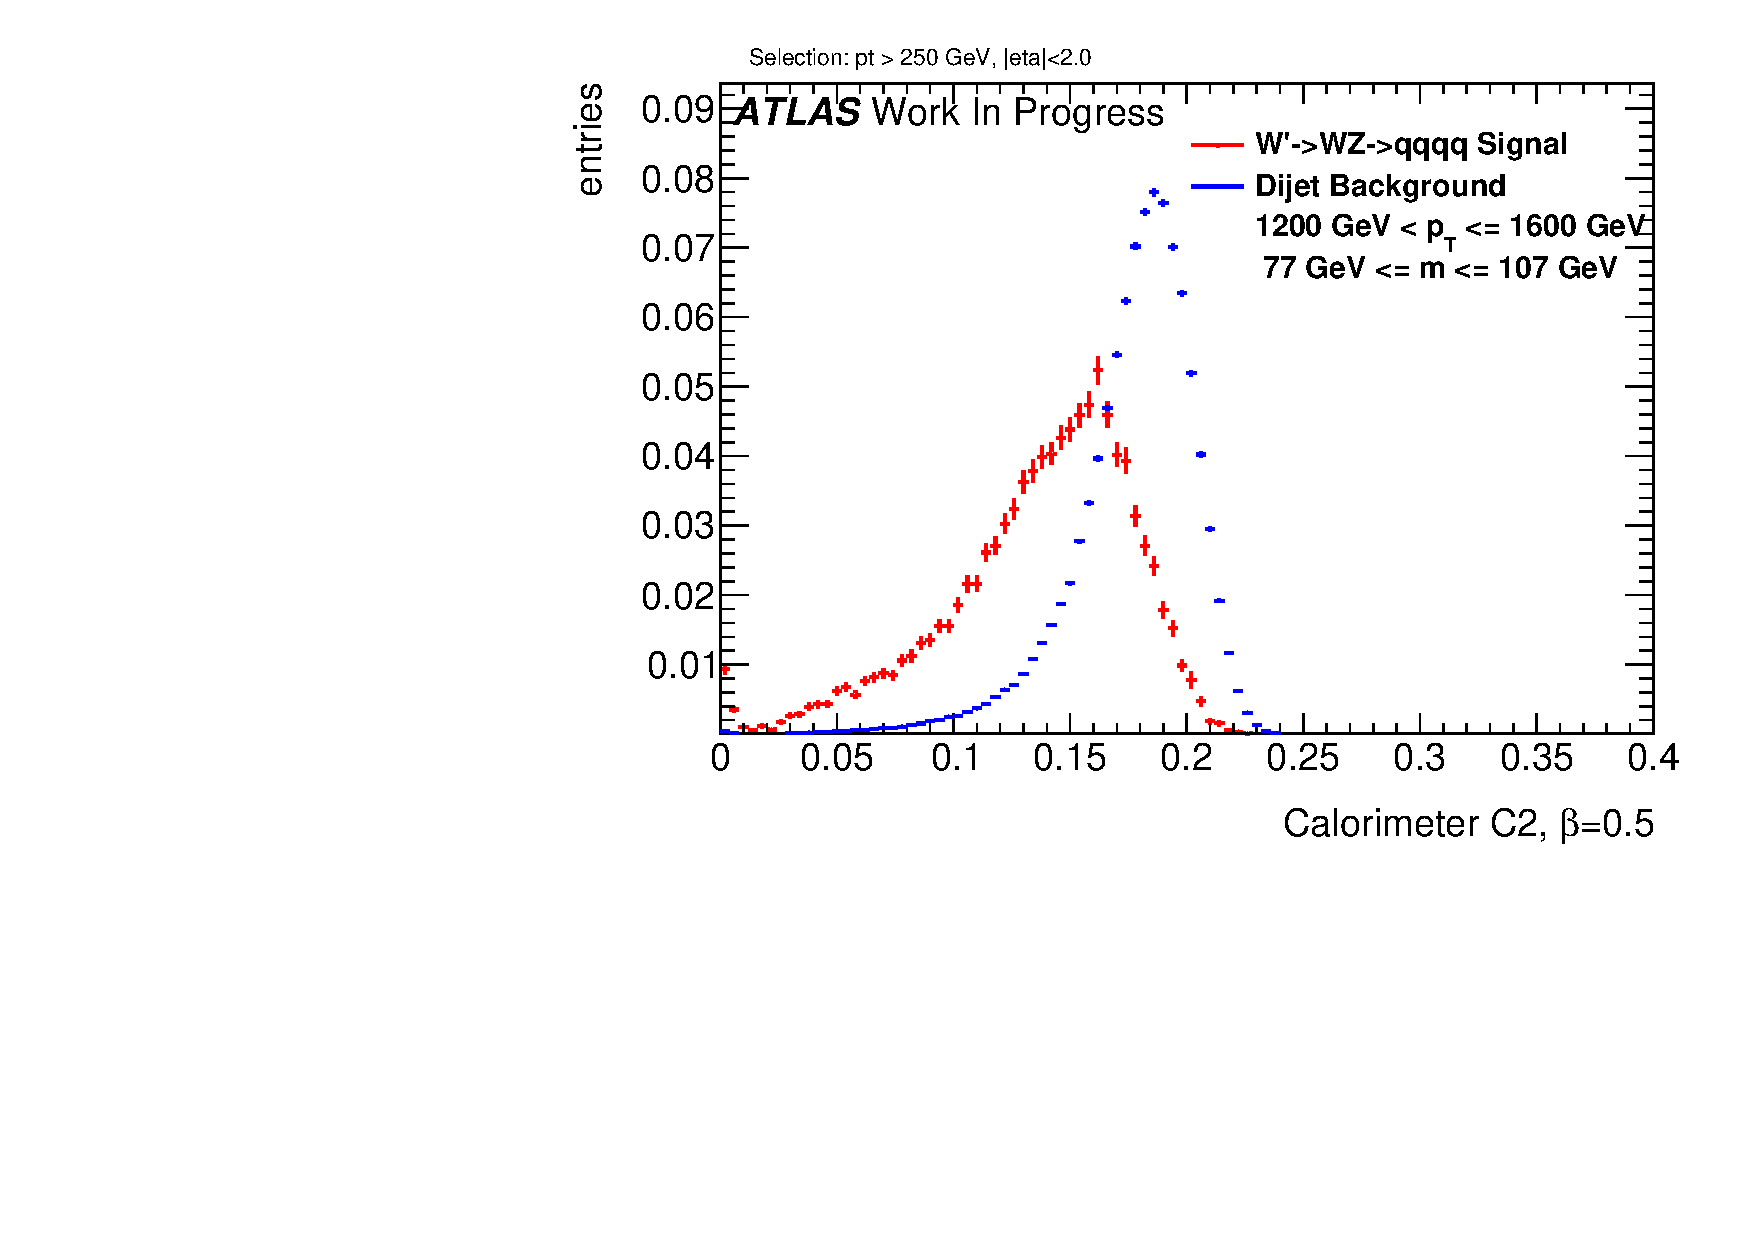
\includegraphics[width=0.3\textwidth]{sascha_input/Appendix/Distributions/w/distributions/beta05/h_recoJet_C2_05_bin4.pdf} \hspace{1mm}
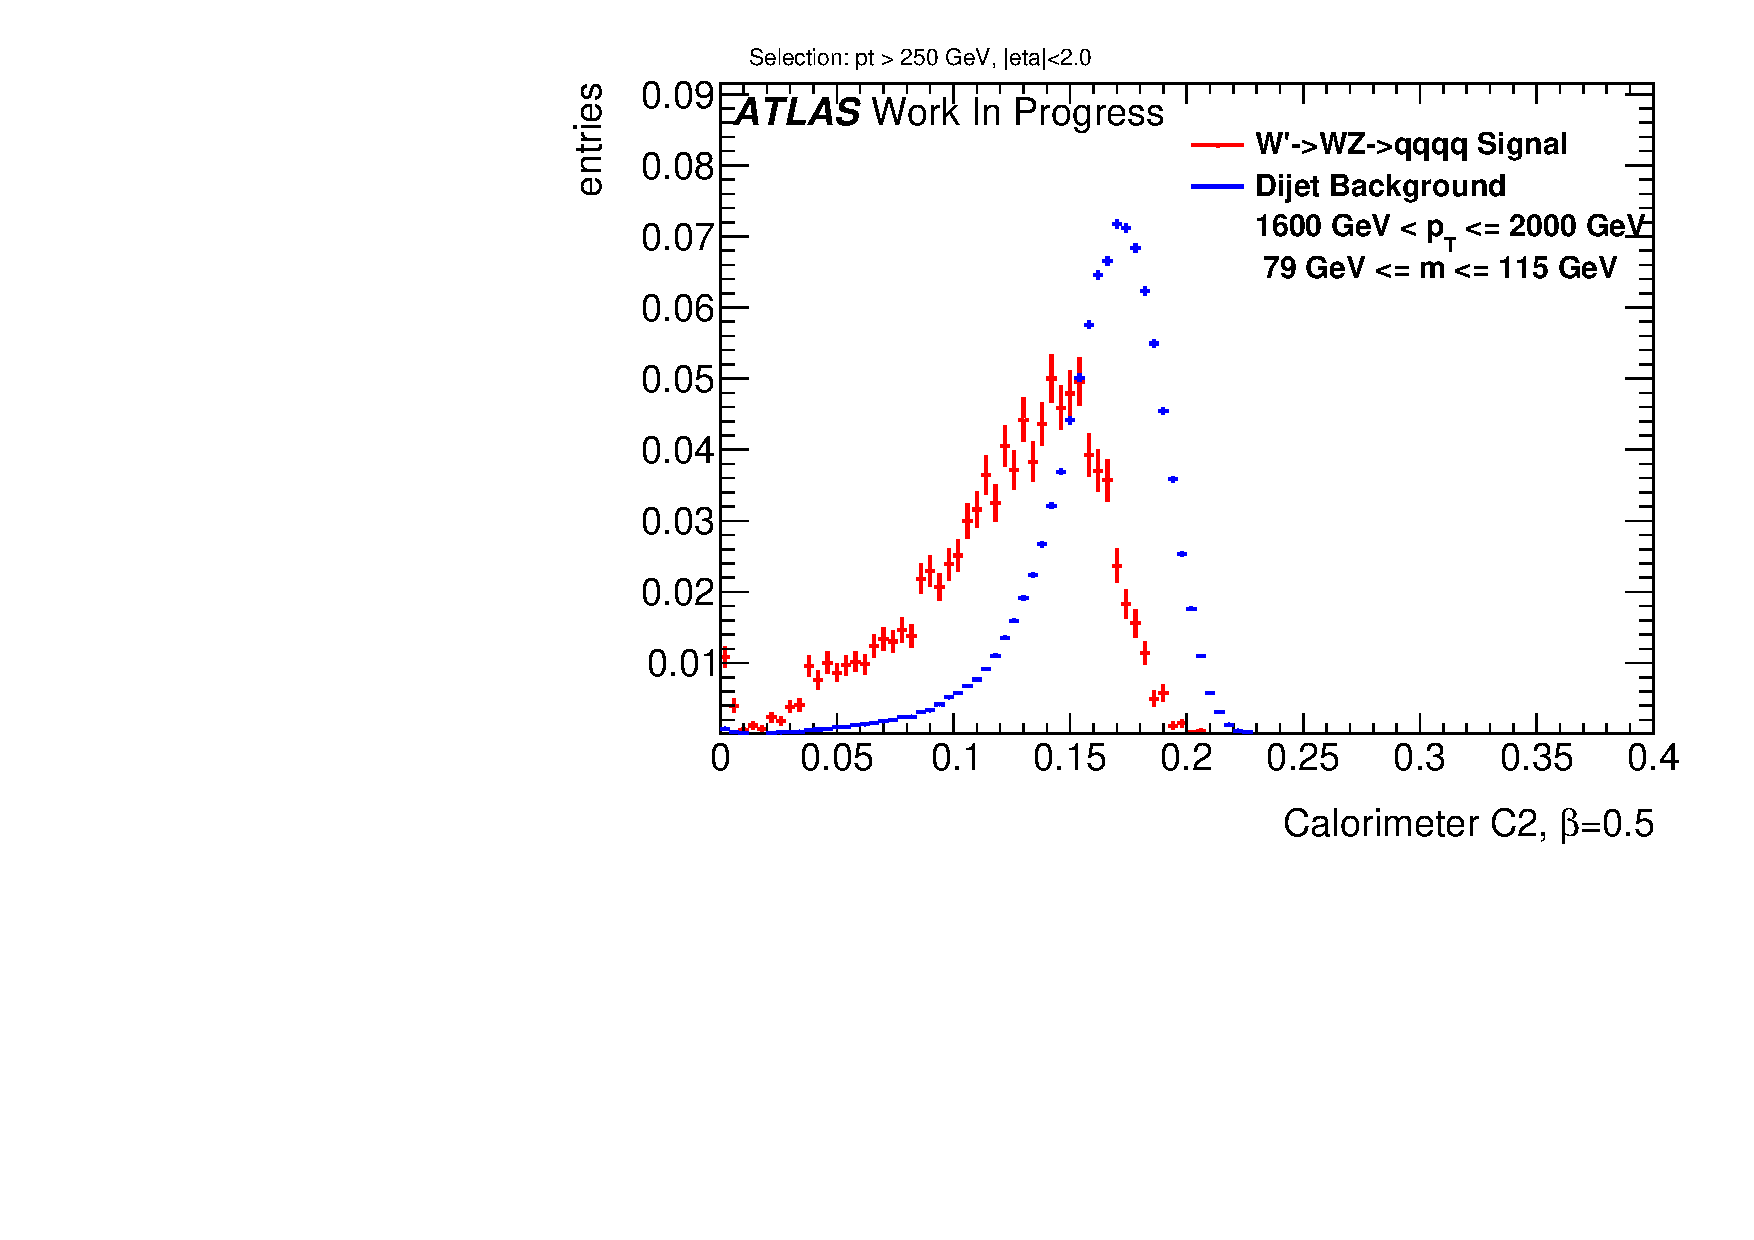
\includegraphics[width=0.3\textwidth]{sascha_input/Appendix/Distributions/w/distributions/beta05/h_recoJet_C2_05_bin5.pdf} \hspace{1mm}
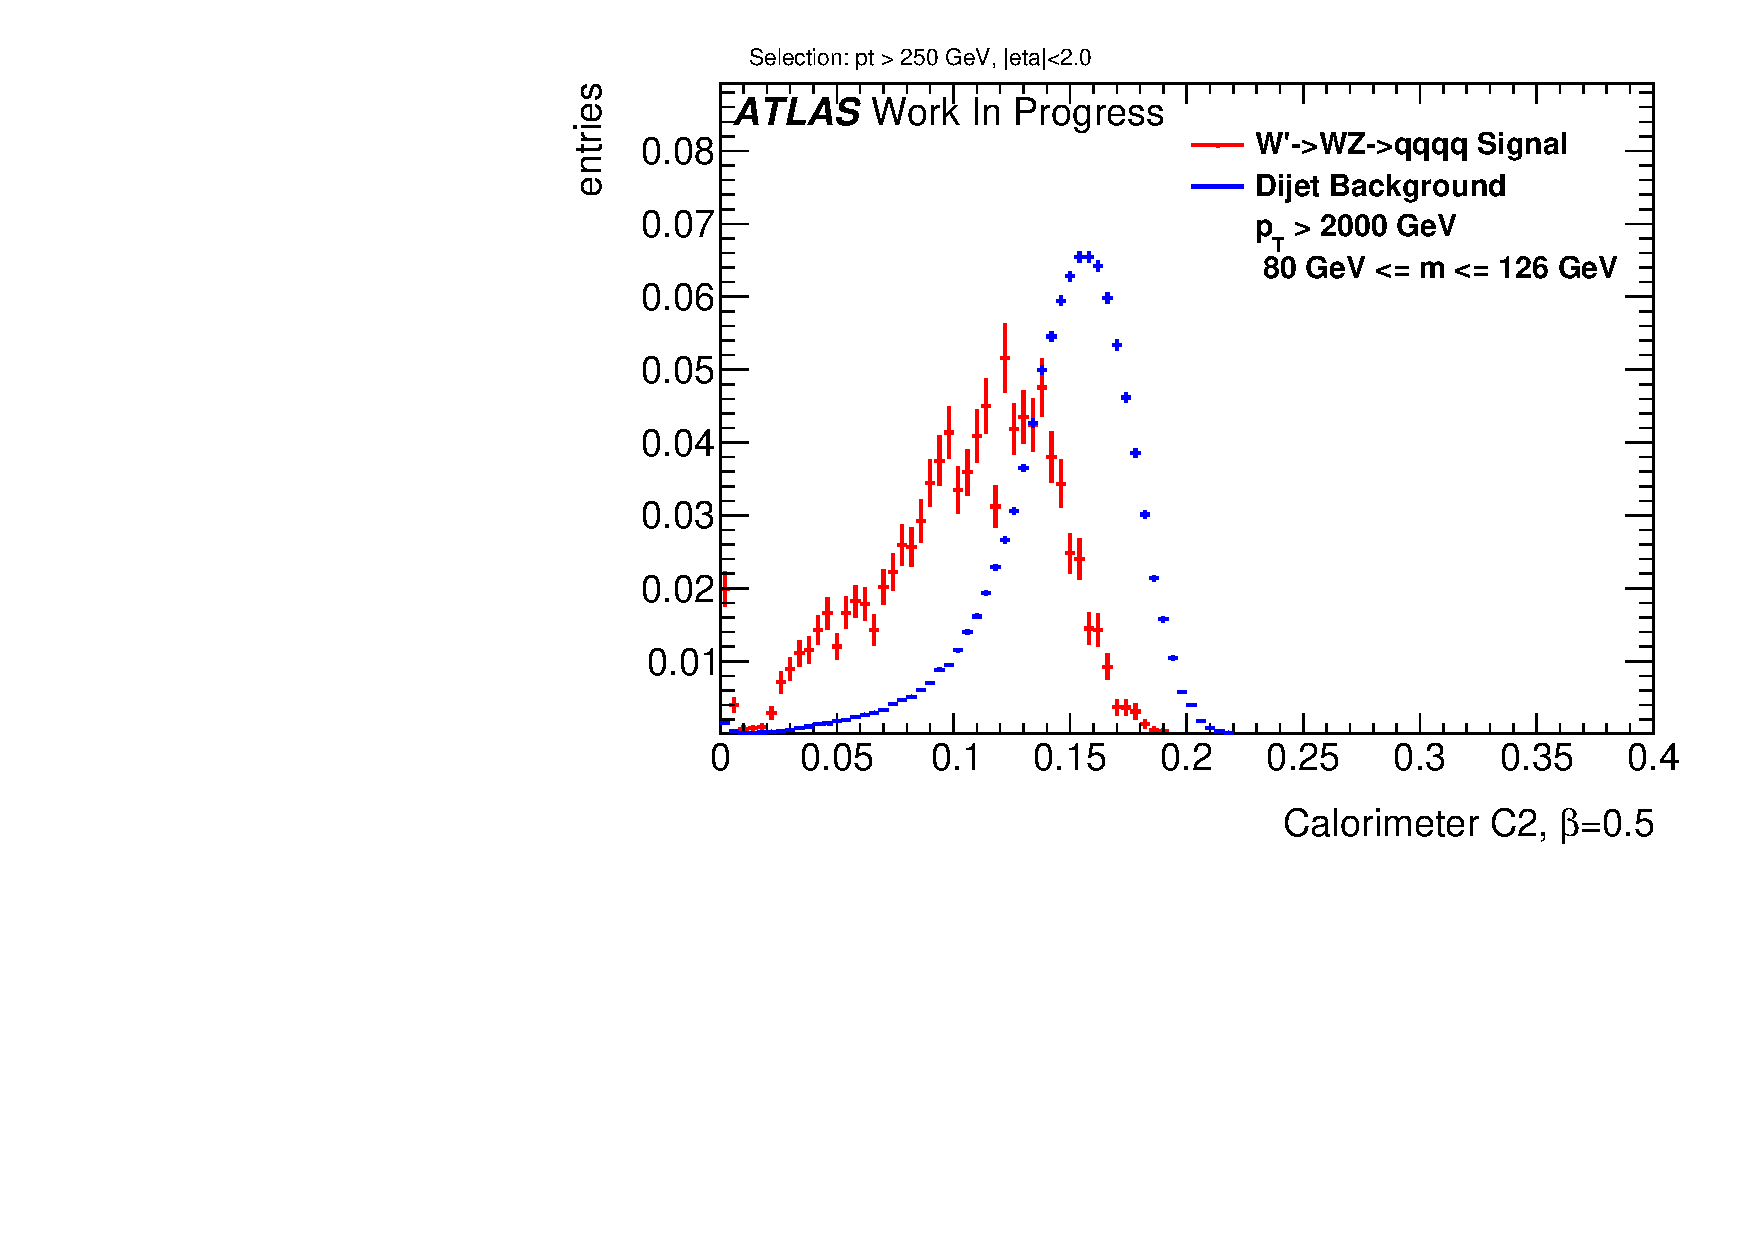
\includegraphics[width=0.3\textwidth]{sascha_input/Appendix/Distributions/w/distributions/beta05/h_recoJet_C2_05_bin6.pdf}
\bigskip
\includegraphics[width=0.3\textwidth]{sascha_input/Appendix/Distributions/w/distributions/beta05/h_recoJet_D2_05_bin1.pdf} \hspace{1mm}
\includegraphics[width=0.3\textwidth]{sascha_input/Appendix/Distributions/w/distributions/beta05/h_recoJet_D2_05_bin2.pdf} \hspace{1mm}
\includegraphics[width=0.3\textwidth]{sascha_input/Appendix/Distributions/w/distributions/beta05/h_recoJet_D2_05_bin3.pdf} 
\bigskip
\includegraphics[width=0.3\textwidth]{sascha_input/Appendix/Distributions/w/distributions/beta05/h_recoJet_D2_05_bin4.pdf} \hspace{1mm}
\includegraphics[width=0.3\textwidth]{sascha_input/Appendix/Distributions/w/distributions/beta05/h_recoJet_D2_05_bin5.pdf} \hspace{1mm}
\includegraphics[width=0.3\textwidth]{sascha_input/Appendix/Distributions/w/distributions/beta05/h_recoJet_D2_05_bin6.pdf}
\bigskip
\includegraphics[width=0.3\textwidth]{sascha_input/Appendix/Distributions/w/distributions/beta05/h_recoJet_nSub21_05_bin1.pdf} \hspace{1mm}
\includegraphics[width=0.3\textwidth]{sascha_input/Appendix/Distributions/w/distributions/beta05/h_recoJet_nSub21_05_bin2.pdf} \hspace{1mm}
\includegraphics[width=0.3\textwidth]{sascha_input/Appendix/Distributions/w/distributions/beta05/h_recoJet_nSub21_05_bin3.pdf} 
\bigskip
\includegraphics[width=0.3\textwidth]{sascha_input/Appendix/Distributions/w/distributions/beta05/h_recoJet_nSub21_05_bin4.pdf} \hspace{6mm}
\includegraphics[width=0.3\textwidth]{sascha_input/Appendix/Distributions/w/distributions/beta05/h_recoJet_nSub21_05_bin5.pdf} \hspace{6mm}
\includegraphics[width=0.3\textwidth]{sascha_input/Appendix/Distributions/w/distributions/beta05/h_recoJet_nSub21_05_bin6.pdf}
\caption{{Distributions for $W$ boson tagging using calorimeter clusters $\beta=0.5$. C2, D2, $\tau_{21}$ top down.}}
\end{figure}
\subsubsection*{$\beta=1$}\label{subsec:app_w_1}
\vspace{-0.5cm}
\begin{figure}[H]
\includegraphics[width=0.3\textwidth]{sascha_input/Appendix/Distributions/w/distributions/beta1/h_assisted_tj_C2_bin1.pdf} \hspace{1mm}
\includegraphics[width=0.3\textwidth]{sascha_input/Appendix/Distributions/w/distributions/beta1/h_assisted_tj_C2_bin2.pdf} \hspace{1mm}
\includegraphics[width=0.3\textwidth]{sascha_input/Appendix/Distributions/w/distributions/beta1/h_assisted_tj_C2_bin3.pdf} 
\bigskip
\includegraphics[width=0.3\textwidth]{sascha_input/Appendix/Distributions/w/distributions/beta1/h_assisted_tj_C2_bin4.pdf} \hspace{1mm}
\includegraphics[width=0.3\textwidth]{sascha_input/Appendix/Distributions/w/distributions/beta1/h_assisted_tj_C2_bin5.pdf} \hspace{1mm}
\includegraphics[width=0.3\textwidth]{sascha_input/Appendix/Distributions/w/distributions/beta1/h_assisted_tj_C2_bin6.pdf} 
\bigskip
\includegraphics[width=0.3\textwidth]{sascha_input/Appendix/Distributions/w/distributions/beta1/h_assisted_tj_D2_bin1.pdf} \hspace{1mm}
\includegraphics[width=0.3\textwidth]{sascha_input/Appendix/Distributions/w/distributions/beta1/h_assisted_tj_D2_bin2.pdf} \hspace{1mm}
\includegraphics[width=0.3\textwidth]{sascha_input/Appendix/Distributions/w/distributions/beta1/h_assisted_tj_D2_bin3.pdf} 
\bigskip
\includegraphics[width=0.3\textwidth]{sascha_input/Appendix/Distributions/w/distributions/beta1/h_assisted_tj_D2_bin4.pdf} \hspace{1mm}
\includegraphics[width=0.3\textwidth]{sascha_input/Appendix/Distributions/w/distributions/beta1/h_assisted_tj_D2_bin5.pdf} \hspace{1mm}
\includegraphics[width=0.3\textwidth]{sascha_input/Appendix/Distributions/w/distributions/beta1/h_assisted_tj_D2_bin6.pdf}
\bigskip 
\includegraphics[width=0.3\textwidth]{sascha_input/Appendix/Distributions/w/distributions/beta1/h_assisted_tj_nSub21_bin1.pdf} \hspace{1mm}
\includegraphics[width=0.3\textwidth]{sascha_input/Appendix/Distributions/w/distributions/beta1/h_assisted_tj_nSub21_bin2.pdf} \hspace{1mm}
\includegraphics[width=0.3\textwidth]{sascha_input/Appendix/Distributions/w/distributions/beta1/h_assisted_tj_nSub21_bin3.pdf} 
\bigskip
\includegraphics[width=0.3\textwidth]{sascha_input/Appendix/Distributions/w/distributions/beta1/h_assisted_tj_nSub21_bin4.pdf} \hspace{6mm}
\includegraphics[width=0.3\textwidth]{sascha_input/Appendix/Distributions/w/distributions/beta1/h_assisted_tj_nSub21_bin5.pdf} \hspace{6mm}
\includegraphics[width=0.3\textwidth]{sascha_input/Appendix/Distributions/w/distributions/beta1/h_assisted_tj_nSub21_bin6.pdf} 
\vspace{-0.5cm}
\caption{{Distributions for $W$ boson tagging using TAS $\beta=1$. C2, D2, $\tau_{21}$ top down.}}\label{app:W_TAS_1}
\end{figure}
\begin{figure}[H]
\includegraphics[width=0.3\textwidth]{sascha_input/Appendix/Distributions/w/distributions/beta1/h_normal_tj_C2_bin1.pdf} \hspace{1mm}
\includegraphics[width=0.3\textwidth]{sascha_input/Appendix/Distributions/w/distributions/beta1/h_normal_tj_C2_bin2.pdf} \hspace{1mm}
\includegraphics[width=0.3\textwidth]{sascha_input/Appendix/Distributions/w/distributions/beta1/h_normal_tj_C2_bin3.pdf} 
\bigskip
\includegraphics[width=0.3\textwidth]{sascha_input/Appendix/Distributions/w/distributions/beta1/h_normal_tj_C2_bin4.pdf} \hspace{1mm}
\includegraphics[width=0.3\textwidth]{sascha_input/Appendix/Distributions/w/distributions/beta1/h_normal_tj_C2_bin5.pdf} \hspace{1mm}
\includegraphics[width=0.3\textwidth]{sascha_input/Appendix/Distributions/w/distributions/beta1/h_normal_tj_C2_bin6.pdf} 
\bigskip
\includegraphics[width=0.3\textwidth]{sascha_input/Appendix/Distributions/w/distributions/beta1/h_normal_tj_D2_bin1.pdf} \hspace{1mm}
\includegraphics[width=0.3\textwidth]{sascha_input/Appendix/Distributions/w/distributions/beta1/h_normal_tj_D2_bin2.pdf} \hspace{1mm}
\includegraphics[width=0.3\textwidth]{sascha_input/Appendix/Distributions/w/distributions/beta1/h_normal_tj_D2_bin3.pdf} 
\bigskip
\includegraphics[width=0.3\textwidth]{sascha_input/Appendix/Distributions/w/distributions/beta1/h_normal_tj_D2_bin4.pdf} \hspace{1mm}
\includegraphics[width=0.3\textwidth]{sascha_input/Appendix/Distributions/w/distributions/beta1/h_normal_tj_D2_bin5.pdf} \hspace{1mm}
\includegraphics[width=0.3\textwidth]{sascha_input/Appendix/Distributions/w/distributions/beta1/h_normal_tj_D2_bin6.pdf}
\bigskip
\includegraphics[width=0.3\textwidth]{sascha_input/Appendix/Distributions/w/distributions/beta1/h_normal_tj_nSub21_bin1.pdf} \hspace{1mm}
\includegraphics[width=0.3\textwidth]{sascha_input/Appendix/Distributions/w/distributions/beta1/h_normal_tj_nSub21_bin2.pdf} \hspace{1mm}
\includegraphics[width=0.3\textwidth]{sascha_input/Appendix/Distributions/w/distributions/beta1/h_normal_tj_nSub21_bin3.pdf} 
\bigskip
\includegraphics[width=0.3\textwidth]{sascha_input/Appendix/Distributions/w/distributions/beta1/h_normal_tj_nSub21_bin4.pdf} \hspace{6mm}
\includegraphics[width=0.3\textwidth]{sascha_input/Appendix/Distributions/w/distributions/beta1/h_normal_tj_nSub21_bin5.pdf} \hspace{6mm}
\includegraphics[width=0.3\textwidth]{sascha_input/Appendix/Distributions/w/distributions/beta1/h_normal_tj_nSub21_bin6.pdf}
\caption{{Distributions for $W$ boson tagging using tracks $\beta=1$. C2, D2, $\tau_{21}$ top down.}}\label{app:W_track_1}
\end{figure}
\begin{figure}[H]
\includegraphics[width=0.3\textwidth]{sascha_input/Appendix/Distributions/w/distributions/beta1/h_recoJet_C2_bin1.pdf} \hspace{1mm}
\includegraphics[width=0.3\textwidth]{sascha_input/Appendix/Distributions/w/distributions/beta1/h_recoJet_C2_bin2.pdf} \hspace{1mm}
\includegraphics[width=0.3\textwidth]{sascha_input/Appendix/Distributions/w/distributions/beta1/h_recoJet_C2_bin3.pdf} 
\bigskip
\includegraphics[width=0.3\textwidth]{sascha_input/Appendix/Distributions/w/distributions/beta1/h_recoJet_C2_bin4.pdf} \hspace{1mm}
\includegraphics[width=0.3\textwidth]{sascha_input/Appendix/Distributions/w/distributions/beta1/h_recoJet_C2_bin5.pdf} \hspace{1mm}
\includegraphics[width=0.3\textwidth]{sascha_input/Appendix/Distributions/w/distributions/beta1/h_recoJet_C2_bin6.pdf}
\bigskip
\includegraphics[width=0.3\textwidth]{sascha_input/Appendix/Distributions/w/distributions/beta1/h_recoJet_D2_bin1.pdf} \hspace{1mm}
\includegraphics[width=0.3\textwidth]{sascha_input/Appendix/Distributions/w/distributions/beta1/h_recoJet_D2_bin2.pdf} \hspace{1mm}
\includegraphics[width=0.3\textwidth]{sascha_input/Appendix/Distributions/w/distributions/beta1/h_recoJet_D2_bin3.pdf} 
\bigskip
\includegraphics[width=0.3\textwidth]{sascha_input/Appendix/Distributions/w/distributions/beta1/h_recoJet_D2_bin4.pdf} \hspace{1mm}
\includegraphics[width=0.3\textwidth]{sascha_input/Appendix/Distributions/w/distributions/beta1/h_recoJet_D2_bin5.pdf} \hspace{1mm}
\includegraphics[width=0.3\textwidth]{sascha_input/Appendix/Distributions/w/distributions/beta1/h_recoJet_D2_bin6.pdf}
\bigskip
\includegraphics[width=0.3\textwidth]{sascha_input/Appendix/Distributions/w/distributions/beta1/h_recoJet_nSub21_bin1.pdf} \hspace{1mm}
\includegraphics[width=0.3\textwidth]{sascha_input/Appendix/Distributions/w/distributions/beta1/h_recoJet_nSub21_bin2.pdf} \hspace{1mm}
\includegraphics[width=0.3\textwidth]{sascha_input/Appendix/Distributions/w/distributions/beta1/h_recoJet_nSub21_bin3.pdf} 
\bigskip
\includegraphics[width=0.3\textwidth]{sascha_input/Appendix/Distributions/w/distributions/beta1/h_recoJet_nSub21_bin4.pdf} \hspace{6mm}
\includegraphics[width=0.3\textwidth]{sascha_input/Appendix/Distributions/w/distributions/beta1/h_recoJet_nSub21_bin5.pdf} \hspace{6mm}
\includegraphics[width=0.3\textwidth]{sascha_input/Appendix/Distributions/w/distributions/beta1/h_recoJet_nSub21_bin6.pdf}
\caption{{Distributions for $W$ boson tagging using calorimeter clusters $\beta=1$. C2, D2, $\tau_{21}$ top down.}}\label{app:W_calo_1}
\end{figure}
\subsubsection*{$\beta=1.7$}
\begin{figure}[H]
\includegraphics[width=0.3\textwidth]{sascha_input/Appendix/Distributions/w/distributions/beta17/h_assisted_tj_C2_17_bin1.pdf} \hspace{1mm}
\includegraphics[width=0.3\textwidth]{sascha_input/Appendix/Distributions/w/distributions/beta17/h_assisted_tj_C2_17_bin2.pdf} \hspace{1mm}
\includegraphics[width=0.3\textwidth]{sascha_input/Appendix/Distributions/w/distributions/beta17/h_assisted_tj_C2_17_bin3.pdf} 
\bigskip
\includegraphics[width=0.3\textwidth]{sascha_input/Appendix/Distributions/w/distributions/beta17/h_assisted_tj_C2_17_bin4.pdf} \hspace{1mm}
\includegraphics[width=0.3\textwidth]{sascha_input/Appendix/Distributions/w/distributions/beta17/h_assisted_tj_C2_17_bin5.pdf} \hspace{1mm}
\includegraphics[width=0.3\textwidth]{sascha_input/Appendix/Distributions/w/distributions/beta17/h_assisted_tj_C2_17_bin6.pdf} 
\bigskip
\includegraphics[width=0.3\textwidth]{sascha_input/Appendix/Distributions/w/distributions/beta17/h_assisted_tj_D2_17_bin1.pdf} \hspace{1mm}
\includegraphics[width=0.3\textwidth]{sascha_input/Appendix/Distributions/w/distributions/beta17/h_assisted_tj_D2_17_bin2.pdf} \hspace{1mm}
\includegraphics[width=0.3\textwidth]{sascha_input/Appendix/Distributions/w/distributions/beta17/h_assisted_tj_D2_17_bin3.pdf} 
\bigskip
\includegraphics[width=0.3\textwidth]{sascha_input/Appendix/Distributions/w/distributions/beta17/h_assisted_tj_D2_17_bin4.pdf} \hspace{1mm}
\includegraphics[width=0.3\textwidth]{sascha_input/Appendix/Distributions/w/distributions/beta17/h_assisted_tj_D2_17_bin5.pdf} \hspace{1mm}
\includegraphics[width=0.3\textwidth]{sascha_input/Appendix/Distributions/w/distributions/beta17/h_assisted_tj_D2_17_bin6.pdf}
\bigskip 
\includegraphics[width=0.3\textwidth]{sascha_input/Appendix/Distributions/w/distributions/beta17/h_assisted_tj_nSub21_17_bin1.pdf} \hspace{1mm}
\includegraphics[width=0.3\textwidth]{sascha_input/Appendix/Distributions/w/distributions/beta17/h_assisted_tj_nSub21_17_bin2.pdf} \hspace{1mm}
\includegraphics[width=0.3\textwidth]{sascha_input/Appendix/Distributions/w/distributions/beta17/h_assisted_tj_nSub21_17_bin3.pdf} 
\bigskip
\includegraphics[width=0.3\textwidth]{sascha_input/Appendix/Distributions/w/distributions/beta17/h_assisted_tj_nSub21_17_bin4.pdf} \hspace{6mm}
\includegraphics[width=0.3\textwidth]{sascha_input/Appendix/Distributions/w/distributions/beta17/h_assisted_tj_nSub21_17_bin5.pdf} \hspace{6mm}
\includegraphics[width=0.3\textwidth]{sascha_input/Appendix/Distributions/w/distributions/beta17/h_assisted_tj_nSub21_17_bin6.pdf} 
\caption{{Distributions for $W$ boson tagging using TAS $\beta=1.7$. C2, D2, $\tau_{21}$ top down.}} \label{app:W_TAS_17}
\end{figure}
\begin{figure}[H]
\includegraphics[width=0.3\textwidth]{sascha_input/Appendix/Distributions/w/distributions/beta17/h_normal_tj_C2_17_bin1.pdf} \hspace{1mm}
\includegraphics[width=0.3\textwidth]{sascha_input/Appendix/Distributions/w/distributions/beta17/h_normal_tj_C2_17_bin2.pdf} \hspace{1mm}
\includegraphics[width=0.3\textwidth]{sascha_input/Appendix/Distributions/w/distributions/beta17/h_normal_tj_C2_17_bin3.pdf} 
\bigskip
\includegraphics[width=0.3\textwidth]{sascha_input/Appendix/Distributions/w/distributions/beta17/h_normal_tj_C2_17_bin4.pdf} \hspace{1mm}
\includegraphics[width=0.3\textwidth]{sascha_input/Appendix/Distributions/w/distributions/beta17/h_normal_tj_C2_17_bin5.pdf} \hspace{1mm}
\includegraphics[width=0.3\textwidth]{sascha_input/Appendix/Distributions/w/distributions/beta17/h_normal_tj_C2_17_bin6.pdf} 
\bigskip
\includegraphics[width=0.3\textwidth]{sascha_input/Appendix/Distributions/w/distributions/beta17/h_normal_tj_D2_17_bin1.pdf} \hspace{1mm}
\includegraphics[width=0.3\textwidth]{sascha_input/Appendix/Distributions/w/distributions/beta17/h_normal_tj_D2_17_bin2.pdf} \hspace{1mm}
\includegraphics[width=0.3\textwidth]{sascha_input/Appendix/Distributions/w/distributions/beta17/h_normal_tj_D2_17_bin3.pdf} 
\bigskip
\includegraphics[width=0.3\textwidth]{sascha_input/Appendix/Distributions/w/distributions/beta17/h_normal_tj_D2_17_bin4.pdf} \hspace{1mm}
\includegraphics[width=0.3\textwidth]{sascha_input/Appendix/Distributions/w/distributions/beta17/h_normal_tj_D2_17_bin5.pdf} \hspace{1mm}
\includegraphics[width=0.3\textwidth]{sascha_input/Appendix/Distributions/w/distributions/beta17/h_normal_tj_D2_17_bin6.pdf}
\bigskip
\includegraphics[width=0.3\textwidth]{sascha_input/Appendix/Distributions/w/distributions/beta17/h_normal_tj_nSub21_17_bin1.pdf} \hspace{1mm}
\includegraphics[width=0.3\textwidth]{sascha_input/Appendix/Distributions/w/distributions/beta17/h_normal_tj_nSub21_17_bin2.pdf} \hspace{1mm}
\includegraphics[width=0.3\textwidth]{sascha_input/Appendix/Distributions/w/distributions/beta17/h_normal_tj_nSub21_17_bin3.pdf} 
\bigskip
\includegraphics[width=0.3\textwidth]{sascha_input/Appendix/Distributions/w/distributions/beta17/h_normal_tj_nSub21_17_bin4.pdf} \hspace{6mm}
\includegraphics[width=0.3\textwidth]{sascha_input/Appendix/Distributions/w/distributions/beta17/h_normal_tj_nSub21_17_bin5.pdf} \hspace{6mm}
\includegraphics[width=0.3\textwidth]{sascha_input/Appendix/Distributions/w/distributions/beta17/h_normal_tj_nSub21_17_bin6.pdf}
\caption{{Distributions for $W$ boson tagging using tracks $\beta=1.7$. C2, D2, $\tau_{21}$ top down.}}\label{app:W_track_17}
\end{figure}
\begin{figure}[H]
\includegraphics[width=0.3\textwidth]{sascha_input/Appendix/Distributions/w/distributions/beta17/h_recoJet_C2_17_bin1.pdf} \hspace{1mm}
\includegraphics[width=0.3\textwidth]{sascha_input/Appendix/Distributions/w/distributions/beta17/h_recoJet_C2_17_bin2.pdf} \hspace{1mm}
\includegraphics[width=0.3\textwidth]{sascha_input/Appendix/Distributions/w/distributions/beta17/h_recoJet_C2_17_bin3.pdf} 
\bigskip
\includegraphics[width=0.3\textwidth]{sascha_input/Appendix/Distributions/w/distributions/beta17/h_recoJet_C2_17_bin4.pdf} \hspace{1mm}
\includegraphics[width=0.3\textwidth]{sascha_input/Appendix/Distributions/w/distributions/beta17/h_recoJet_C2_17_bin5.pdf} \hspace{1mm}
\includegraphics[width=0.3\textwidth]{sascha_input/Appendix/Distributions/w/distributions/beta17/h_recoJet_C2_17_bin6.pdf}
\bigskip
\includegraphics[width=0.3\textwidth]{sascha_input/Appendix/Distributions/w/distributions/beta17/h_recoJet_D2_17_bin1.pdf} \hspace{1mm}
\includegraphics[width=0.3\textwidth]{sascha_input/Appendix/Distributions/w/distributions/beta17/h_recoJet_D2_17_bin2.pdf} \hspace{1mm}
\includegraphics[width=0.3\textwidth]{sascha_input/Appendix/Distributions/w/distributions/beta17/h_recoJet_D2_17_bin3.pdf} 
\bigskip
\includegraphics[width=0.3\textwidth]{sascha_input/Appendix/Distributions/w/distributions/beta17/h_recoJet_D2_17_bin4.pdf} \hspace{1mm}
\includegraphics[width=0.3\textwidth]{sascha_input/Appendix/Distributions/w/distributions/beta17/h_recoJet_D2_17_bin5.pdf} \hspace{1mm}
\includegraphics[width=0.3\textwidth]{sascha_input/Appendix/Distributions/w/distributions/beta17/h_recoJet_D2_17_bin6.pdf}
\bigskip
\includegraphics[width=0.3\textwidth]{sascha_input/Appendix/Distributions/w/distributions/beta17/h_recoJet_nSub21_17_bin1.pdf} \hspace{1mm}
\includegraphics[width=0.3\textwidth]{sascha_input/Appendix/Distributions/w/distributions/beta17/h_recoJet_nSub21_17_bin2.pdf} \hspace{1mm}
\includegraphics[width=0.3\textwidth]{sascha_input/Appendix/Distributions/w/distributions/beta17/h_recoJet_nSub21_17_bin3.pdf} 
\bigskip
\includegraphics[width=0.3\textwidth]{sascha_input/Appendix/Distributions/w/distributions/beta17/h_recoJet_nSub21_17_bin4.pdf} \hspace{6mm}
\includegraphics[width=0.3\textwidth]{sascha_input/Appendix/Distributions/w/distributions/beta17/h_recoJet_nSub21_17_bin5.pdf} \hspace{6mm}
\includegraphics[width=0.3\textwidth]{sascha_input/Appendix/Distributions/w/distributions/beta17/h_recoJet_nSub21_17_bin6.pdf}
\caption{{Distributions for $W$ boson tagging using calorimeter clusters $\beta=1.7$. C2, D2, $\tau_{21}$ top down.}}
\end{figure}
\subsubsection*{$\beta=2$}
\begin{figure}[H]
\includegraphics[width=0.3\textwidth]{sascha_input/Appendix/Distributions/w/distributions/beta2/h_assisted_tj_C2_2_bin1.pdf} \hspace{1mm}
\includegraphics[width=0.3\textwidth]{sascha_input/Appendix/Distributions/w/distributions/beta2/h_assisted_tj_C2_2_bin2.pdf} \hspace{1mm}
\includegraphics[width=0.3\textwidth]{sascha_input/Appendix/Distributions/w/distributions/beta2/h_assisted_tj_C2_2_bin3.pdf} 
\bigskip
\includegraphics[width=0.3\textwidth]{sascha_input/Appendix/Distributions/w/distributions/beta2/h_assisted_tj_C2_2_bin4.pdf} \hspace{1mm}
\includegraphics[width=0.3\textwidth]{sascha_input/Appendix/Distributions/w/distributions/beta2/h_assisted_tj_C2_2_bin5.pdf} \hspace{1mm}
\includegraphics[width=0.3\textwidth]{sascha_input/Appendix/Distributions/w/distributions/beta2/h_assisted_tj_C2_2_bin6.pdf} 
\bigskip
\includegraphics[width=0.3\textwidth]{sascha_input/Appendix/Distributions/w/distributions/beta2/h_assisted_tj_D2_2_bin1.pdf} \hspace{1mm}
\includegraphics[width=0.3\textwidth]{sascha_input/Appendix/Distributions/w/distributions/beta2/h_assisted_tj_D2_2_bin2.pdf} \hspace{1mm}
\includegraphics[width=0.3\textwidth]{sascha_input/Appendix/Distributions/w/distributions/beta2/h_assisted_tj_D2_2_bin3.pdf} 
\bigskip
\includegraphics[width=0.3\textwidth]{sascha_input/Appendix/Distributions/w/distributions/beta2/h_assisted_tj_D2_2_bin4.pdf} \hspace{1mm}
\includegraphics[width=0.3\textwidth]{sascha_input/Appendix/Distributions/w/distributions/beta2/h_assisted_tj_D2_2_bin5.pdf} \hspace{1mm}
\includegraphics[width=0.3\textwidth]{sascha_input/Appendix/Distributions/w/distributions/beta2/h_assisted_tj_D2_2_bin6.pdf}
\bigskip 
\includegraphics[width=0.3\textwidth]{sascha_input/Appendix/Distributions/w/distributions/beta2/h_assisted_tj_nSub21_2_bin1.pdf} \hspace{1mm}
\includegraphics[width=0.3\textwidth]{sascha_input/Appendix/Distributions/w/distributions/beta2/h_assisted_tj_nSub21_2_bin2.pdf} \hspace{1mm}
\includegraphics[width=0.3\textwidth]{sascha_input/Appendix/Distributions/w/distributions/beta2/h_assisted_tj_nSub21_2_bin3.pdf} 
\bigskip
\includegraphics[width=0.3\textwidth]{sascha_input/Appendix/Distributions/w/distributions/beta2/h_assisted_tj_nSub21_2_bin4.pdf} \hspace{6mm}
\includegraphics[width=0.3\textwidth]{sascha_input/Appendix/Distributions/w/distributions/beta2/h_assisted_tj_nSub21_2_bin5.pdf} \hspace{6mm}
\includegraphics[width=0.3\textwidth]{sascha_input/Appendix/Distributions/w/distributions/beta2/h_assisted_tj_nSub21_2_bin6.pdf} 
\caption{{Distributions for $W$ boson tagging using TAS $\beta=2$. C2, D2, $\tau_{21}$ top down.}}
\end{figure}
\begin{figure}[H]
\includegraphics[width=0.3\textwidth]{sascha_input/Appendix/Distributions/w/distributions/beta2/h_normal_tj_C2_2_bin1.pdf} \hspace{1mm}
\includegraphics[width=0.3\textwidth]{sascha_input/Appendix/Distributions/w/distributions/beta2/h_normal_tj_C2_2_bin2.pdf} \hspace{1mm}
\includegraphics[width=0.3\textwidth]{sascha_input/Appendix/Distributions/w/distributions/beta2/h_normal_tj_C2_2_bin3.pdf} 
\bigskip
\includegraphics[width=0.3\textwidth]{sascha_input/Appendix/Distributions/w/distributions/beta2/h_normal_tj_C2_2_bin4.pdf} \hspace{1mm}
\includegraphics[width=0.3\textwidth]{sascha_input/Appendix/Distributions/w/distributions/beta2/h_normal_tj_C2_2_bin5.pdf} \hspace{1mm}
\includegraphics[width=0.3\textwidth]{sascha_input/Appendix/Distributions/w/distributions/beta2/h_normal_tj_C2_2_bin6.pdf} 
\bigskip
\includegraphics[width=0.3\textwidth]{sascha_input/Appendix/Distributions/w/distributions/beta2/h_normal_tj_D2_2_bin1.pdf} \hspace{1mm}
\includegraphics[width=0.3\textwidth]{sascha_input/Appendix/Distributions/w/distributions/beta2/h_normal_tj_D2_2_bin2.pdf} \hspace{1mm}
\includegraphics[width=0.3\textwidth]{sascha_input/Appendix/Distributions/w/distributions/beta2/h_normal_tj_D2_2_bin3.pdf} 
\bigskip
\includegraphics[width=0.3\textwidth]{sascha_input/Appendix/Distributions/w/distributions/beta2/h_normal_tj_D2_2_bin4.pdf} \hspace{1mm}
\includegraphics[width=0.3\textwidth]{sascha_input/Appendix/Distributions/w/distributions/beta2/h_normal_tj_D2_2_bin5.pdf} \hspace{1mm}
\includegraphics[width=0.3\textwidth]{sascha_input/Appendix/Distributions/w/distributions/beta2/h_normal_tj_D2_2_bin6.pdf}
\bigskip
\includegraphics[width=0.3\textwidth]{sascha_input/Appendix/Distributions/w/distributions/beta2/h_normal_tj_nSub21_2_bin1.pdf} \hspace{1mm}
\includegraphics[width=0.3\textwidth]{sascha_input/Appendix/Distributions/w/distributions/beta2/h_normal_tj_nSub21_2_bin2.pdf} \hspace{1mm}
\includegraphics[width=0.3\textwidth]{sascha_input/Appendix/Distributions/w/distributions/beta2/h_normal_tj_nSub21_2_bin3.pdf} 
\bigskip
\includegraphics[width=0.3\textwidth]{sascha_input/Appendix/Distributions/w/distributions/beta2/h_normal_tj_nSub21_2_bin4.pdf} \hspace{6mm}
\includegraphics[width=0.3\textwidth]{sascha_input/Appendix/Distributions/w/distributions/beta2/h_normal_tj_nSub21_2_bin5.pdf} \hspace{6mm}
\includegraphics[width=0.3\textwidth]{sascha_input/Appendix/Distributions/w/distributions/beta2/h_normal_tj_nSub21_2_bin6.pdf}
\caption{{Distributions for $W$ boson tagging using tracks $\beta=2$. C2, D2, $\tau_{21}$ top down.}}
\end{figure}
\begin{figure}[H]
\includegraphics[width=0.3\textwidth]{sascha_input/Appendix/Distributions/w/distributions/beta2/h_recoJet_C2_2_bin1.pdf} \hspace{1mm}
\includegraphics[width=0.3\textwidth]{sascha_input/Appendix/Distributions/w/distributions/beta2/h_recoJet_C2_2_bin2.pdf} \hspace{1mm}
\includegraphics[width=0.3\textwidth]{sascha_input/Appendix/Distributions/w/distributions/beta2/h_recoJet_C2_2_bin3.pdf} 
\bigskip
\includegraphics[width=0.3\textwidth]{sascha_input/Appendix/Distributions/w/distributions/beta2/h_recoJet_C2_2_bin4.pdf} \hspace{1mm}
\includegraphics[width=0.3\textwidth]{sascha_input/Appendix/Distributions/w/distributions/beta2/h_recoJet_C2_2_bin5.pdf} \hspace{1mm}
\includegraphics[width=0.3\textwidth]{sascha_input/Appendix/Distributions/w/distributions/beta2/h_recoJet_C2_2_bin6.pdf}
\bigskip
\includegraphics[width=0.3\textwidth]{sascha_input/Appendix/Distributions/w/distributions/beta2/h_recoJet_D2_2_bin1.pdf} \hspace{1mm}
\includegraphics[width=0.3\textwidth]{sascha_input/Appendix/Distributions/w/distributions/beta2/h_recoJet_D2_2_bin2.pdf} \hspace{1mm}
\includegraphics[width=0.3\textwidth]{sascha_input/Appendix/Distributions/w/distributions/beta2/h_recoJet_D2_2_bin3.pdf} 
\bigskip
\includegraphics[width=0.3\textwidth]{sascha_input/Appendix/Distributions/w/distributions/beta2/h_recoJet_D2_2_bin4.pdf} \hspace{1mm}
\includegraphics[width=0.3\textwidth]{sascha_input/Appendix/Distributions/w/distributions/beta2/h_recoJet_D2_2_bin5.pdf} \hspace{1mm}
\includegraphics[width=0.3\textwidth]{sascha_input/Appendix/Distributions/w/distributions/beta2/h_recoJet_D2_2_bin6.pdf}
\bigskip
\includegraphics[width=0.3\textwidth]{sascha_input/Appendix/Distributions/w/distributions/beta2/h_recoJet_nSub21_2_bin1.pdf} \hspace{1mm}
\includegraphics[width=0.3\textwidth]{sascha_input/Appendix/Distributions/w/distributions/beta2/h_recoJet_nSub21_2_bin2.pdf} \hspace{1mm}
\includegraphics[width=0.3\textwidth]{sascha_input/Appendix/Distributions/w/distributions/beta2/h_recoJet_nSub21_2_bin3.pdf} 
\bigskip
\includegraphics[width=0.3\textwidth]{sascha_input/Appendix/Distributions/w/distributions/beta2/h_recoJet_nSub21_2_bin4.pdf} \hspace{6mm}
\includegraphics[width=0.3\textwidth]{sascha_input/Appendix/Distributions/w/distributions/beta2/h_recoJet_nSub21_2_bin5.pdf} \hspace{6mm}
\includegraphics[width=0.3\textwidth]{sascha_input/Appendix/Distributions/w/distributions/beta2/h_recoJet_nSub21_2_bin6.pdf}
\caption{{Distributions for $W$ boson tagging using calorimeter clusters $\beta=2$. C2, D2, $\tau_{21}$ top down.}}
\end{figure}
\subsubsection*{$\beta=3$}
\begin{figure}[H]
\includegraphics[width=0.3\textwidth]{sascha_input/Appendix/Distributions/w/distributions/beta3/h_assisted_tj_C2_3_bin1.pdf} \hspace{1mm}
\includegraphics[width=0.3\textwidth]{sascha_input/Appendix/Distributions/w/distributions/beta3/h_assisted_tj_C2_3_bin2.pdf} \hspace{1mm}
\includegraphics[width=0.3\textwidth]{sascha_input/Appendix/Distributions/w/distributions/beta3/h_assisted_tj_C2_3_bin3.pdf} 
\bigskip
\includegraphics[width=0.3\textwidth]{sascha_input/Appendix/Distributions/w/distributions/beta3/h_assisted_tj_C2_3_bin4.pdf} \hspace{1mm}
\includegraphics[width=0.3\textwidth]{sascha_input/Appendix/Distributions/w/distributions/beta3/h_assisted_tj_C2_3_bin5.pdf} \hspace{1mm}
\includegraphics[width=0.3\textwidth]{sascha_input/Appendix/Distributions/w/distributions/beta3/h_assisted_tj_C2_3_bin6.pdf} 
\bigskip
\includegraphics[width=0.3\textwidth]{sascha_input/Appendix/Distributions/w/distributions/beta3/h_assisted_tj_D2_3_bin1.pdf} \hspace{1mm}
\includegraphics[width=0.3\textwidth]{sascha_input/Appendix/Distributions/w/distributions/beta3/h_assisted_tj_D2_3_bin2.pdf} \hspace{1mm}
\includegraphics[width=0.3\textwidth]{sascha_input/Appendix/Distributions/w/distributions/beta3/h_assisted_tj_D2_3_bin3.pdf} 
\bigskip
\includegraphics[width=0.3\textwidth]{sascha_input/Appendix/Distributions/w/distributions/beta3/h_assisted_tj_D2_3_bin4.pdf} \hspace{1mm}
\includegraphics[width=0.3\textwidth]{sascha_input/Appendix/Distributions/w/distributions/beta3/h_assisted_tj_D2_3_bin5.pdf} \hspace{1mm}
\includegraphics[width=0.3\textwidth]{sascha_input/Appendix/Distributions/w/distributions/beta3/h_assisted_tj_D2_3_bin6.pdf}
\bigskip 
\includegraphics[width=0.3\textwidth]{sascha_input/Appendix/Distributions/w/distributions/beta3/h_assisted_tj_nSub21_3_bin1.pdf} \hspace{1mm}
\includegraphics[width=0.3\textwidth]{sascha_input/Appendix/Distributions/w/distributions/beta3/h_assisted_tj_nSub21_3_bin2.pdf} \hspace{1mm}
\includegraphics[width=0.3\textwidth]{sascha_input/Appendix/Distributions/w/distributions/beta3/h_assisted_tj_nSub21_3_bin3.pdf} 
\bigskip
\includegraphics[width=0.3\textwidth]{sascha_input/Appendix/Distributions/w/distributions/beta3/h_assisted_tj_nSub21_3_bin4.pdf} \hspace{6mm}
\includegraphics[width=0.3\textwidth]{sascha_input/Appendix/Distributions/w/distributions/beta3/h_assisted_tj_nSub21_3_bin5.pdf} \hspace{6mm}
\includegraphics[width=0.3\textwidth]{sascha_input/Appendix/Distributions/w/distributions/beta3/h_assisted_tj_nSub21_3_bin6.pdf} 
\caption{{Distributions for $W$ boson tagging using TAS $\beta=3$. C2, D2, $\tau_{21}$ top down.}}
\end{figure}
\begin{figure}[H]
\includegraphics[width=0.3\textwidth]{sascha_input/Appendix/Distributions/w/distributions/beta3/h_normal_tj_C2_3_bin1.pdf} \hspace{1mm}
\includegraphics[width=0.3\textwidth]{sascha_input/Appendix/Distributions/w/distributions/beta3/h_normal_tj_C2_3_bin2.pdf} \hspace{1mm}
\includegraphics[width=0.3\textwidth]{sascha_input/Appendix/Distributions/w/distributions/beta3/h_normal_tj_C2_3_bin3.pdf} 
\bigskip
\includegraphics[width=0.3\textwidth]{sascha_input/Appendix/Distributions/w/distributions/beta3/h_normal_tj_C2_3_bin4.pdf} \hspace{1mm}
\includegraphics[width=0.3\textwidth]{sascha_input/Appendix/Distributions/w/distributions/beta3/h_normal_tj_C2_3_bin5.pdf} \hspace{1mm}
\includegraphics[width=0.3\textwidth]{sascha_input/Appendix/Distributions/w/distributions/beta3/h_normal_tj_C2_3_bin6.pdf} 
\bigskip
\includegraphics[width=0.3\textwidth]{sascha_input/Appendix/Distributions/w/distributions/beta3/h_normal_tj_D2_3_bin1.pdf} \hspace{1mm}
\includegraphics[width=0.3\textwidth]{sascha_input/Appendix/Distributions/w/distributions/beta3/h_normal_tj_D2_3_bin2.pdf} \hspace{1mm}
\includegraphics[width=0.3\textwidth]{sascha_input/Appendix/Distributions/w/distributions/beta3/h_normal_tj_D2_3_bin3.pdf} 
\bigskip
\includegraphics[width=0.3\textwidth]{sascha_input/Appendix/Distributions/w/distributions/beta3/h_normal_tj_D2_3_bin4.pdf} \hspace{1mm}
\includegraphics[width=0.3\textwidth]{sascha_input/Appendix/Distributions/w/distributions/beta3/h_normal_tj_D2_3_bin5.pdf} \hspace{1mm}
\includegraphics[width=0.3\textwidth]{sascha_input/Appendix/Distributions/w/distributions/beta3/h_normal_tj_D2_3_bin6.pdf}
\bigskip
\includegraphics[width=0.3\textwidth]{sascha_input/Appendix/Distributions/w/distributions/beta3/h_normal_tj_nSub21_3_bin1.pdf} \hspace{1mm}
\includegraphics[width=0.3\textwidth]{sascha_input/Appendix/Distributions/w/distributions/beta3/h_normal_tj_nSub21_3_bin2.pdf} \hspace{1mm}
\includegraphics[width=0.3\textwidth]{sascha_input/Appendix/Distributions/w/distributions/beta3/h_normal_tj_nSub21_3_bin3.pdf} 
\bigskip
\includegraphics[width=0.3\textwidth]{sascha_input/Appendix/Distributions/w/distributions/beta3/h_normal_tj_nSub21_3_bin4.pdf} \hspace{6mm}
\includegraphics[width=0.3\textwidth]{sascha_input/Appendix/Distributions/w/distributions/beta3/h_normal_tj_nSub21_3_bin5.pdf} \hspace{6mm}
\includegraphics[width=0.3\textwidth]{sascha_input/Appendix/Distributions/w/distributions/beta3/h_normal_tj_nSub21_3_bin6.pdf}
\caption{{Distributions for $W$ boson tagging using tracks $\beta=3$. C2, D2, $\tau_{21}$ top down.}}
\end{figure}
\begin{figure}[H]
\includegraphics[width=0.3\textwidth]{sascha_input/Appendix/Distributions/w/distributions/beta3/h_recoJet_C2_3_bin1.pdf} \hspace{1mm}
\includegraphics[width=0.3\textwidth]{sascha_input/Appendix/Distributions/w/distributions/beta3/h_recoJet_C2_3_bin2.pdf} \hspace{1mm}
\includegraphics[width=0.3\textwidth]{sascha_input/Appendix/Distributions/w/distributions/beta3/h_recoJet_C2_3_bin3.pdf} 
\bigskip
\includegraphics[width=0.3\textwidth]{sascha_input/Appendix/Distributions/w/distributions/beta3/h_recoJet_C2_3_bin4.pdf} \hspace{1mm}
\includegraphics[width=0.3\textwidth]{sascha_input/Appendix/Distributions/w/distributions/beta3/h_recoJet_C2_3_bin5.pdf} \hspace{1mm}
\includegraphics[width=0.3\textwidth]{sascha_input/Appendix/Distributions/w/distributions/beta3/h_recoJet_C2_3_bin6.pdf}
\bigskip
\includegraphics[width=0.3\textwidth]{sascha_input/Appendix/Distributions/w/distributions/beta3/h_recoJet_D2_3_bin1.pdf} \hspace{1mm}
\includegraphics[width=0.3\textwidth]{sascha_input/Appendix/Distributions/w/distributions/beta3/h_recoJet_D2_3_bin2.pdf} \hspace{1mm}
\includegraphics[width=0.3\textwidth]{sascha_input/Appendix/Distributions/w/distributions/beta3/h_recoJet_D2_3_bin3.pdf} 
\bigskip
\includegraphics[width=0.3\textwidth]{sascha_input/Appendix/Distributions/w/distributions/beta3/h_recoJet_D2_3_bin4.pdf} \hspace{1mm}
\includegraphics[width=0.3\textwidth]{sascha_input/Appendix/Distributions/w/distributions/beta3/h_recoJet_D2_3_bin5.pdf} \hspace{1mm}
\includegraphics[width=0.3\textwidth]{sascha_input/Appendix/Distributions/w/distributions/beta3/h_recoJet_D2_3_bin6.pdf}
\bigskip
\includegraphics[width=0.3\textwidth]{sascha_input/Appendix/Distributions/w/distributions/beta3/h_recoJet_nSub21_3_bin1.pdf} \hspace{1mm}
\includegraphics[width=0.3\textwidth]{sascha_input/Appendix/Distributions/w/distributions/beta3/h_recoJet_nSub21_3_bin2.pdf} \hspace{1mm}
\includegraphics[width=0.3\textwidth]{sascha_input/Appendix/Distributions/w/distributions/beta3/h_recoJet_nSub21_3_bin3.pdf} 
\bigskip
\includegraphics[width=0.3\textwidth]{sascha_input/Appendix/Distributions/w/distributions/beta3/h_recoJet_nSub21_3_bin4.pdf} \hspace{6mm}
\includegraphics[width=0.3\textwidth]{sascha_input/Appendix/Distributions/w/distributions/beta3/h_recoJet_nSub21_3_bin5.pdf} \hspace{6mm}
\includegraphics[width=0.3\textwidth]{sascha_input/Appendix/Distributions/w/distributions/beta3/h_recoJet_nSub21_3_bin6.pdf}
\caption{{Distributions for $W$ boson tagging using calorimeter clusters $\beta=3$. C2, D2, $\tau_{21}$ top down.}}
\end{figure}


\subsection{Higgs Distributions}
\subsubsection*{$\beta=0.5$}
\begin{figure}[H]
\includegraphics[width=0.3\textwidth]{sascha_input/Appendix/Distributions/higgs/distributions/beta05/h_assisted_tj_C2_05_bin1.pdf} \hspace{1mm}
\includegraphics[width=0.3\textwidth]{sascha_input/Appendix/Distributions/higgs/distributions/beta05/h_assisted_tj_C2_05_bin2.pdf} \hspace{4mm}
\includegraphics[width=0.3\textwidth]{sascha_input/Appendix/Distributions/higgs/distributions/beta05/h_assisted_tj_C2_05_bin3.pdf} 
\bigskip
\includegraphics[width=0.3\textwidth]{sascha_input/Appendix/Distributions/higgs/distributions/beta05/h_assisted_tj_C2_05_bin4.pdf} \hspace{4mm}
\includegraphics[width=0.3\textwidth]{sascha_input/Appendix/Distributions/higgs/distributions/beta05/h_assisted_tj_C2_05_bin5.pdf} 

\bigskip
\includegraphics[width=0.3\textwidth]{sascha_input/Appendix/Distributions/higgs/distributions/beta05/h_assisted_tj_D2_05_bin1.pdf} \hspace{1mm}
\includegraphics[width=0.3\textwidth]{sascha_input/Appendix/Distributions/higgs/distributions/beta05/h_assisted_tj_D2_05_bin2.pdf} \hspace{4mm}
\includegraphics[width=0.3\textwidth]{sascha_input/Appendix/Distributions/higgs/distributions/beta05/h_assisted_tj_D2_05_bin3.pdf} 
\bigskip
\includegraphics[width=0.3\textwidth]{sascha_input/Appendix/Distributions/higgs/distributions/beta05/h_assisted_tj_D2_05_bin4.pdf} \hspace{4mm}
\includegraphics[width=0.3\textwidth]{sascha_input/Appendix/Distributions/higgs/distributions/beta05/h_assisted_tj_D2_05_bin5.pdf} 

\bigskip 
\includegraphics[width=0.3\textwidth]{sascha_input/Appendix/Distributions/higgs/distributions/beta05/h_assisted_tj_nSub21_05_bin1.pdf} \hspace{1mm}
\includegraphics[width=0.3\textwidth]{sascha_input/Appendix/Distributions/higgs/distributions/beta05/h_assisted_tj_nSub21_05_bin2.pdf} \hspace{4mm}
\includegraphics[width=0.3\textwidth]{sascha_input/Appendix/Distributions/higgs/distributions/beta05/h_assisted_tj_nSub21_05_bin3.pdf} 
\bigskip
\includegraphics[width=0.3\textwidth]{sascha_input/Appendix/Distributions/higgs/distributions/beta05/h_assisted_tj_nSub21_05_bin4.pdf} \hspace{4mm}
\includegraphics[width=0.3\textwidth]{sascha_input/Appendix/Distributions/higgs/distributions/beta05/h_assisted_tj_nSub21_05_bin5.pdf} 
\vspace{-0.75cm}
\caption{{Distributions for Higgs boson tagging using TAS $\beta=0.5$. C2, D2, $\tau_{21}$ top down.}}
\end{figure}
\begin{figure}[H]
\includegraphics[width=0.3\textwidth]{sascha_input/Appendix/Distributions/higgs/distributions/beta05/h_normal_tj_C2_05_bin1.pdf} 	\hspace{1mm}
\includegraphics[width=0.3\textwidth]{sascha_input/Appendix/Distributions/higgs/distributions/beta05/h_normal_tj_C2_05_bin2.pdf} 	\hspace{4mm}
\includegraphics[width=0.3\textwidth]{sascha_input/Appendix/Distributions/higgs/distributions/beta05/h_normal_tj_C2_05_bin3.pdf} 
\bigskip
\includegraphics[width=0.3\textwidth]{sascha_input/Appendix/Distributions/higgs/distributions/beta05/h_normal_tj_C2_05_bin4.pdf} 	\hspace{4mm}
\includegraphics[width=0.3\textwidth]{sascha_input/Appendix/Distributions/higgs/distributions/beta05/h_normal_tj_C2_05_bin5.pdf} 

\bigskip
\includegraphics[width=0.3\textwidth]{sascha_input/Appendix/Distributions/higgs/distributions/beta05/h_normal_tj_D2_05_bin1.pdf} 	\hspace{1mm}
\includegraphics[width=0.3\textwidth]{sascha_input/Appendix/Distributions/higgs/distributions/beta05/h_normal_tj_D2_05_bin2.pdf} 	\hspace{4mm}
\includegraphics[width=0.3\textwidth]{sascha_input/Appendix/Distributions/higgs/distributions/beta05/h_normal_tj_D2_05_bin3.pdf} 
\bigskip
\includegraphics[width=0.3\textwidth]{sascha_input/Appendix/Distributions/higgs/distributions/beta05/h_normal_tj_D2_05_bin4.pdf} 	\hspace{4mm}
\includegraphics[width=0.3\textwidth]{sascha_input/Appendix/Distributions/higgs/distributions/beta05/h_normal_tj_D2_05_bin5.pdf} 

\bigskip
\includegraphics[width=0.3\textwidth]{sascha_input/Appendix/Distributions/higgs/distributions/beta05/h_normal_tj_nSub21_05_bin1.pdf} 	\hspace{1mm}
\includegraphics[width=0.3\textwidth]{sascha_input/Appendix/Distributions/higgs/distributions/beta05/h_normal_tj_nSub21_05_bin2.pdf} 	\hspace{4mm}
\includegraphics[width=0.3\textwidth]{sascha_input/Appendix/Distributions/higgs/distributions/beta05/h_normal_tj_nSub21_05_bin3.pdf} 
\bigskip
\includegraphics[width=0.3\textwidth]{sascha_input/Appendix/Distributions/higgs/distributions/beta05/h_normal_tj_nSub21_05_bin4.pdf} \hspace{4mm}
\includegraphics[width=0.3\textwidth]{sascha_input/Appendix/Distributions/higgs/distributions/beta05/h_normal_tj_nSub21_05_bin5.pdf} 

\caption{{Distributions for Higgs boson tagging using tracks $\beta=0.5$. C2, D2, $\tau_{21}$ top down.}}
\end{figure}
\begin{figure}[H]
\includegraphics[width=0.3\textwidth]{sascha_input/Appendix/Distributions/higgs/distributions/beta05/h_recoJet_C2_05_bin1.pdf} \hspace{1mm}
\includegraphics[width=0.3\textwidth]{sascha_input/Appendix/Distributions/higgs/distributions/beta05/h_recoJet_C2_05_bin2.pdf} \hspace{4mm}
\includegraphics[width=0.3\textwidth]{sascha_input/Appendix/Distributions/higgs/distributions/beta05/h_recoJet_C2_05_bin3.pdf} 
\bigskip
\includegraphics[width=0.3\textwidth]{sascha_input/Appendix/Distributions/higgs/distributions/beta05/h_recoJet_C2_05_bin4.pdf} \hspace{4mm}
\includegraphics[width=0.3\textwidth]{sascha_input/Appendix/Distributions/higgs/distributions/beta05/h_recoJet_C2_05_bin5.pdf} 

\bigskip
\includegraphics[width=0.3\textwidth]{sascha_input/Appendix/Distributions/higgs/distributions/beta05/h_recoJet_D2_05_bin1.pdf} \hspace{1mm}
\includegraphics[width=0.3\textwidth]{sascha_input/Appendix/Distributions/higgs/distributions/beta05/h_recoJet_D2_05_bin2.pdf} \hspace{4mm}
\includegraphics[width=0.3\textwidth]{sascha_input/Appendix/Distributions/higgs/distributions/beta05/h_recoJet_D2_05_bin3.pdf} 
\bigskip
\includegraphics[width=0.3\textwidth]{sascha_input/Appendix/Distributions/higgs/distributions/beta05/h_recoJet_D2_05_bin4.pdf} \hspace{4mm}
\includegraphics[width=0.3\textwidth]{sascha_input/Appendix/Distributions/higgs/distributions/beta05/h_recoJet_D2_05_bin5.pdf} 

\bigskip
\includegraphics[width=0.3\textwidth]{sascha_input/Appendix/Distributions/higgs/distributions/beta05/h_recoJet_nSub21_05_bin1.pdf} \hspace{1mm}
\includegraphics[width=0.3\textwidth]{sascha_input/Appendix/Distributions/higgs/distributions/beta05/h_recoJet_nSub21_05_bin2.pdf} \hspace{4mm}
\includegraphics[width=0.3\textwidth]{sascha_input/Appendix/Distributions/higgs/distributions/beta05/h_recoJet_nSub21_05_bin3.pdf} 
\bigskip
\includegraphics[width=0.3\textwidth]{sascha_input/Appendix/Distributions/higgs/distributions/beta05/h_recoJet_nSub21_05_bin4.pdf} \hspace{4mm}
\includegraphics[width=0.3\textwidth]{sascha_input/Appendix/Distributions/higgs/distributions/beta05/h_recoJet_nSub21_05_bin5.pdf} 

\caption{{Distributions for Higgs boson tagging using calorimeter clusters $\beta=0.5$. C2, D2, $\tau_{21}$ top down.}}
\end{figure}
\subsubsection*{$\beta=1$}
\begin{figure}[H]
\includegraphics[width=0.3\textwidth]{sascha_input/Appendix/Distributions/higgs/distributions/beta1/h_assisted_tj_C2_bin1.pdf} \hspace{1mm}
\includegraphics[width=0.3\textwidth]{sascha_input/Appendix/Distributions/higgs/distributions/beta1/h_assisted_tj_C2_bin2.pdf} \hspace{4mm}
\includegraphics[width=0.3\textwidth]{sascha_input/Appendix/Distributions/higgs/distributions/beta1/h_assisted_tj_C2_bin3.pdf} 
\bigskip
\includegraphics[width=0.3\textwidth]{sascha_input/Appendix/Distributions/higgs/distributions/beta1/h_assisted_tj_C2_bin4.pdf} \hspace{4mm}
\includegraphics[width=0.3\textwidth]{sascha_input/Appendix/Distributions/higgs/distributions/beta1/h_assisted_tj_C2_bin5.pdf} 

\bigskip
\includegraphics[width=0.3\textwidth]{sascha_input/Appendix/Distributions/higgs/distributions/beta1/h_assisted_tj_D2_bin1.pdf} \hspace{1mm}
\includegraphics[width=0.3\textwidth]{sascha_input/Appendix/Distributions/higgs/distributions/beta1/h_assisted_tj_D2_bin2.pdf} \hspace{4mm}
\includegraphics[width=0.3\textwidth]{sascha_input/Appendix/Distributions/higgs/distributions/beta1/h_assisted_tj_D2_bin3.pdf} 
\bigskip
\includegraphics[width=0.3\textwidth]{sascha_input/Appendix/Distributions/higgs/distributions/beta1/h_assisted_tj_D2_bin4.pdf} \hspace{4mm}
\includegraphics[width=0.3\textwidth]{sascha_input/Appendix/Distributions/higgs/distributions/beta1/h_assisted_tj_D2_bin5.pdf} 

\bigskip 
\includegraphics[width=0.3\textwidth]{sascha_input/Appendix/Distributions/higgs/distributions/beta1/h_assisted_tj_nSub21_bin1.pdf} \hspace{1mm}
\includegraphics[width=0.3\textwidth]{sascha_input/Appendix/Distributions/higgs/distributions/beta1/h_assisted_tj_nSub21_bin2.pdf} \hspace{4mm}
\includegraphics[width=0.3\textwidth]{sascha_input/Appendix/Distributions/higgs/distributions/beta1/h_assisted_tj_nSub21_bin3.pdf} 
\bigskip
\includegraphics[width=0.3\textwidth]{sascha_input/Appendix/Distributions/higgs/distributions/beta1/h_assisted_tj_nSub21_bin4.pdf} \hspace{4mm}
\includegraphics[width=0.3\textwidth]{sascha_input/Appendix/Distributions/higgs/distributions/beta1/h_assisted_tj_nSub21_bin5.pdf} 

\vspace{-0.5cm}
\caption{{Distributions for Higgs boson tagging using TAS $\beta=1$. C2, D2, $\tau_{21}$ top down.}}
\end{figure}
\begin{figure}[H]
\includegraphics[width=0.3\textwidth]{sascha_input/Appendix/Distributions/higgs/distributions/beta1/h_normal_tj_C2_bin1.pdf} \hspace{1mm}
\includegraphics[width=0.3\textwidth]{sascha_input/Appendix/Distributions/higgs/distributions/beta1/h_normal_tj_C2_bin2.pdf} \hspace{4mm}
\includegraphics[width=0.3\textwidth]{sascha_input/Appendix/Distributions/higgs/distributions/beta1/h_normal_tj_C2_bin3.pdf} 
\bigskip
\includegraphics[width=0.3\textwidth]{sascha_input/Appendix/Distributions/higgs/distributions/beta1/h_normal_tj_C2_bin4.pdf} \hspace{4mm}
\includegraphics[width=0.3\textwidth]{sascha_input/Appendix/Distributions/higgs/distributions/beta1/h_normal_tj_C2_bin5.pdf} 

\bigskip
\includegraphics[width=0.3\textwidth]{sascha_input/Appendix/Distributions/higgs/distributions/beta1/h_normal_tj_D2_bin1.pdf} \hspace{1mm}
\includegraphics[width=0.3\textwidth]{sascha_input/Appendix/Distributions/higgs/distributions/beta1/h_normal_tj_D2_bin2.pdf} \hspace{4mm}
\includegraphics[width=0.3\textwidth]{sascha_input/Appendix/Distributions/higgs/distributions/beta1/h_normal_tj_D2_bin3.pdf} 
\bigskip
\includegraphics[width=0.3\textwidth]{sascha_input/Appendix/Distributions/higgs/distributions/beta1/h_normal_tj_D2_bin4.pdf} \hspace{4mm}
\includegraphics[width=0.3\textwidth]{sascha_input/Appendix/Distributions/higgs/distributions/beta1/h_normal_tj_D2_bin5.pdf} 

\bigskip
\includegraphics[width=0.3\textwidth]{sascha_input/Appendix/Distributions/higgs/distributions/beta1/h_normal_tj_nSub21_bin1.pdf} \hspace{1mm}
\includegraphics[width=0.3\textwidth]{sascha_input/Appendix/Distributions/higgs/distributions/beta1/h_normal_tj_nSub21_bin2.pdf} \hspace{4mm}
\includegraphics[width=0.3\textwidth]{sascha_input/Appendix/Distributions/higgs/distributions/beta1/h_normal_tj_nSub21_bin3.pdf} 
\bigskip
\includegraphics[width=0.3\textwidth]{sascha_input/Appendix/Distributions/higgs/distributions/beta1/h_normal_tj_nSub21_bin4.pdf} \hspace{4mm}
\includegraphics[width=0.3\textwidth]{sascha_input/Appendix/Distributions/higgs/distributions/beta1/h_normal_tj_nSub21_bin5.pdf} 

\caption{{Distributions for Higgs boson tagging using tracks $\beta=1$. C2, D2, $\tau_{21}$ top down.}}
\end{figure}
\begin{figure}[H]
\includegraphics[width=0.3\textwidth]{sascha_input/Appendix/Distributions/higgs/distributions/beta1/h_recoJet_C2_bin1.pdf} \hspace{1mm}
\includegraphics[width=0.3\textwidth]{sascha_input/Appendix/Distributions/higgs/distributions/beta1/h_recoJet_C2_bin2.pdf} \hspace{4mm}
\includegraphics[width=0.3\textwidth]{sascha_input/Appendix/Distributions/higgs/distributions/beta1/h_recoJet_C2_bin3.pdf} 
\bigskip
\includegraphics[width=0.3\textwidth]{sascha_input/Appendix/Distributions/higgs/distributions/beta1/h_recoJet_C2_bin4.pdf} \hspace{4mm}
\includegraphics[width=0.3\textwidth]{sascha_input/Appendix/Distributions/higgs/distributions/beta1/h_recoJet_C2_bin5.pdf} 

\bigskip
\includegraphics[width=0.3\textwidth]{sascha_input/Appendix/Distributions/higgs/distributions/beta1/h_recoJet_D2_bin1.pdf} \hspace{1mm}
\includegraphics[width=0.3\textwidth]{sascha_input/Appendix/Distributions/higgs/distributions/beta1/h_recoJet_D2_bin2.pdf} \hspace{4mm}
\includegraphics[width=0.3\textwidth]{sascha_input/Appendix/Distributions/higgs/distributions/beta1/h_recoJet_D2_bin3.pdf} 
\bigskip
\includegraphics[width=0.3\textwidth]{sascha_input/Appendix/Distributions/higgs/distributions/beta1/h_recoJet_D2_bin4.pdf} \hspace{4mm}
\includegraphics[width=0.3\textwidth]{sascha_input/Appendix/Distributions/higgs/distributions/beta1/h_recoJet_D2_bin5.pdf} 

\bigskip
\includegraphics[width=0.3\textwidth]{sascha_input/Appendix/Distributions/higgs/distributions/beta1/h_recoJet_nSub21_bin1.pdf} \hspace{1mm}
\includegraphics[width=0.3\textwidth]{sascha_input/Appendix/Distributions/higgs/distributions/beta1/h_recoJet_nSub21_bin2.pdf} \hspace{4mm}
\includegraphics[width=0.3\textwidth]{sascha_input/Appendix/Distributions/higgs/distributions/beta1/h_recoJet_nSub21_bin3.pdf} 
\bigskip
\includegraphics[width=0.3\textwidth]{sascha_input/Appendix/Distributions/higgs/distributions/beta1/h_recoJet_nSub21_bin4.pdf} \hspace{4mm}
\includegraphics[width=0.3\textwidth]{sascha_input/Appendix/Distributions/higgs/distributions/beta1/h_recoJet_nSub21_bin5.pdf} 

\caption{{Distributions for Higgs boson tagging using calorimeter clusters $\beta=1$. C2, D2, $\tau_{21}$ top down.}}
\end{figure}
\subsubsection*{$\beta=1.7$}
\begin{figure}[H]
\includegraphics[width=0.3\textwidth]{sascha_input/Appendix/Distributions/higgs/distributions/beta17/h_assisted_tj_C2_17_bin1.pdf} \hspace{1mm}
\includegraphics[width=0.3\textwidth]{sascha_input/Appendix/Distributions/higgs/distributions/beta17/h_assisted_tj_C2_17_bin2.pdf} \hspace{4mm}
\includegraphics[width=0.3\textwidth]{sascha_input/Appendix/Distributions/higgs/distributions/beta17/h_assisted_tj_C2_17_bin3.pdf} 
\bigskip
\includegraphics[width=0.3\textwidth]{sascha_input/Appendix/Distributions/higgs/distributions/beta17/h_assisted_tj_C2_17_bin4.pdf} \hspace{4mm}
\includegraphics[width=0.3\textwidth]{sascha_input/Appendix/Distributions/higgs/distributions/beta17/h_assisted_tj_C2_17_bin5.pdf} 

\bigskip
\includegraphics[width=0.3\textwidth]{sascha_input/Appendix/Distributions/higgs/distributions/beta17/h_assisted_tj_D2_17_bin1.pdf} \hspace{1mm}
\includegraphics[width=0.3\textwidth]{sascha_input/Appendix/Distributions/higgs/distributions/beta17/h_assisted_tj_D2_17_bin2.pdf} \hspace{4mm}
\includegraphics[width=0.3\textwidth]{sascha_input/Appendix/Distributions/higgs/distributions/beta17/h_assisted_tj_D2_17_bin3.pdf} 
\bigskip
\includegraphics[width=0.3\textwidth]{sascha_input/Appendix/Distributions/higgs/distributions/beta17/h_assisted_tj_D2_17_bin4.pdf} \hspace{4mm}
\includegraphics[width=0.3\textwidth]{sascha_input/Appendix/Distributions/higgs/distributions/beta17/h_assisted_tj_D2_17_bin5.pdf} 

\bigskip 
\includegraphics[width=0.3\textwidth]{sascha_input/Appendix/Distributions/higgs/distributions/beta17/h_assisted_tj_nSub21_17_bin1.pdf} \hspace{1mm}
\includegraphics[width=0.3\textwidth]{sascha_input/Appendix/Distributions/higgs/distributions/beta17/h_assisted_tj_nSub21_17_bin2.pdf} \hspace{4mm}
\includegraphics[width=0.3\textwidth]{sascha_input/Appendix/Distributions/higgs/distributions/beta17/h_assisted_tj_nSub21_17_bin3.pdf} 
\bigskip
\includegraphics[width=0.3\textwidth]{sascha_input/Appendix/Distributions/higgs/distributions/beta17/h_assisted_tj_nSub21_17_bin4.pdf} \hspace{4mm}
\includegraphics[width=0.3\textwidth]{sascha_input/Appendix/Distributions/higgs/distributions/beta17/h_assisted_tj_nSub21_17_bin5.pdf} 

\caption{{Distributions for Higgs boson tagging using TAS $\beta=1.7$. C2, D2, $\tau_{21}$ top down.}}
\end{figure}
\begin{figure}[H]
\includegraphics[width=0.3\textwidth]{sascha_input/Appendix/Distributions/higgs/distributions/beta17/h_normal_tj_C2_17_bin1.pdf} \hspace{1mm}
\includegraphics[width=0.3\textwidth]{sascha_input/Appendix/Distributions/higgs/distributions/beta17/h_normal_tj_C2_17_bin2.pdf} \hspace{4mm}
\includegraphics[width=0.3\textwidth]{sascha_input/Appendix/Distributions/higgs/distributions/beta17/h_normal_tj_C2_17_bin3.pdf} 
\bigskip
\includegraphics[width=0.3\textwidth]{sascha_input/Appendix/Distributions/higgs/distributions/beta17/h_normal_tj_C2_17_bin4.pdf} \hspace{4mm}
\includegraphics[width=0.3\textwidth]{sascha_input/Appendix/Distributions/higgs/distributions/beta17/h_normal_tj_C2_17_bin5.pdf} 

\bigskip
\includegraphics[width=0.3\textwidth]{sascha_input/Appendix/Distributions/higgs/distributions/beta17/h_normal_tj_D2_17_bin1.pdf} \hspace{1mm}
\includegraphics[width=0.3\textwidth]{sascha_input/Appendix/Distributions/higgs/distributions/beta17/h_normal_tj_D2_17_bin2.pdf} \hspace{4mm}
\includegraphics[width=0.3\textwidth]{sascha_input/Appendix/Distributions/higgs/distributions/beta17/h_normal_tj_D2_17_bin3.pdf} 
\bigskip
\includegraphics[width=0.3\textwidth]{sascha_input/Appendix/Distributions/higgs/distributions/beta17/h_normal_tj_D2_17_bin4.pdf} \hspace{4mm}
\includegraphics[width=0.3\textwidth]{sascha_input/Appendix/Distributions/higgs/distributions/beta17/h_normal_tj_D2_17_bin5.pdf} 

\bigskip
\includegraphics[width=0.3\textwidth]{sascha_input/Appendix/Distributions/higgs/distributions/beta17/h_normal_tj_nSub21_17_bin1.pdf} \hspace{1mm}
\includegraphics[width=0.3\textwidth]{sascha_input/Appendix/Distributions/higgs/distributions/beta17/h_normal_tj_nSub21_17_bin2.pdf} \hspace{4mm}
\includegraphics[width=0.3\textwidth]{sascha_input/Appendix/Distributions/higgs/distributions/beta17/h_normal_tj_nSub21_17_bin3.pdf} 
\bigskip
\includegraphics[width=0.3\textwidth]{sascha_input/Appendix/Distributions/higgs/distributions/beta17/h_normal_tj_nSub21_17_bin4.pdf} \hspace{4mm}
\includegraphics[width=0.3\textwidth]{sascha_input/Appendix/Distributions/higgs/distributions/beta17/h_normal_tj_nSub21_17_bin5.pdf} 

\caption{{Distributions for Higgs boson tagging using tracks $\beta=1.7$. C2, D2, $\tau_{21}$ top down.}}
\end{figure}
\begin{figure}[H]
\includegraphics[width=0.3\textwidth]{sascha_input/Appendix/Distributions/higgs/distributions/beta17/h_recoJet_C2_17_bin1.pdf} \hspace{1mm}
\includegraphics[width=0.3\textwidth]{sascha_input/Appendix/Distributions/higgs/distributions/beta17/h_recoJet_C2_17_bin2.pdf} \hspace{4mm}
\includegraphics[width=0.3\textwidth]{sascha_input/Appendix/Distributions/higgs/distributions/beta17/h_recoJet_C2_17_bin3.pdf} 
\bigskip
\includegraphics[width=0.3\textwidth]{sascha_input/Appendix/Distributions/higgs/distributions/beta17/h_recoJet_C2_17_bin4.pdf} \hspace{4mm}
\includegraphics[width=0.3\textwidth]{sascha_input/Appendix/Distributions/higgs/distributions/beta17/h_recoJet_C2_17_bin5.pdf} 

\bigskip
\includegraphics[width=0.3\textwidth]{sascha_input/Appendix/Distributions/higgs/distributions/beta17/h_recoJet_D2_17_bin1.pdf} \hspace{1mm}
\includegraphics[width=0.3\textwidth]{sascha_input/Appendix/Distributions/higgs/distributions/beta17/h_recoJet_D2_17_bin2.pdf} \hspace{4mm}
\includegraphics[width=0.3\textwidth]{sascha_input/Appendix/Distributions/higgs/distributions/beta17/h_recoJet_D2_17_bin3.pdf} 
\bigskip
\includegraphics[width=0.3\textwidth]{sascha_input/Appendix/Distributions/higgs/distributions/beta17/h_recoJet_D2_17_bin4.pdf} \hspace{4mm}
\includegraphics[width=0.3\textwidth]{sascha_input/Appendix/Distributions/higgs/distributions/beta17/h_recoJet_D2_17_bin5.pdf} 

\bigskip
\includegraphics[width=0.3\textwidth]{sascha_input/Appendix/Distributions/higgs/distributions/beta17/h_recoJet_nSub21_17_bin1.pdf} \hspace{1mm}
\includegraphics[width=0.3\textwidth]{sascha_input/Appendix/Distributions/higgs/distributions/beta17/h_recoJet_nSub21_17_bin2.pdf} \hspace{4mm}
\includegraphics[width=0.3\textwidth]{sascha_input/Appendix/Distributions/higgs/distributions/beta17/h_recoJet_nSub21_17_bin3.pdf} 
\bigskip
\includegraphics[width=0.3\textwidth]{sascha_input/Appendix/Distributions/higgs/distributions/beta17/h_recoJet_nSub21_17_bin4.pdf} \hspace{4mm}
\includegraphics[width=0.3\textwidth]{sascha_input/Appendix/Distributions/higgs/distributions/beta17/h_recoJet_nSub21_17_bin5.pdf}

\caption{{Distributions for Higgs boson tagging using calorimeter clusters $\beta=1.7$. C2, D2, $\tau_{21}$ top down.}}
\end{figure}
\subsubsection*{$\beta=2$}
\begin{figure}[H]
\includegraphics[width=0.3\textwidth]{sascha_input/Appendix/Distributions/higgs/distributions/beta2/h_assisted_tj_C2_2_bin1.pdf} \hspace{1mm}
\includegraphics[width=0.3\textwidth]{sascha_input/Appendix/Distributions/higgs/distributions/beta2/h_assisted_tj_C2_2_bin2.pdf} \hspace{4mm}
\includegraphics[width=0.3\textwidth]{sascha_input/Appendix/Distributions/higgs/distributions/beta2/h_assisted_tj_C2_2_bin3.pdf} 
\bigskip
\includegraphics[width=0.3\textwidth]{sascha_input/Appendix/Distributions/higgs/distributions/beta2/h_assisted_tj_C2_2_bin4.pdf} \hspace{4mm}
\includegraphics[width=0.3\textwidth]{sascha_input/Appendix/Distributions/higgs/distributions/beta2/h_assisted_tj_C2_2_bin5.pdf} 

\bigskip
\includegraphics[width=0.3\textwidth]{sascha_input/Appendix/Distributions/higgs/distributions/beta2/h_assisted_tj_D2_2_bin1.pdf} \hspace{1mm}
\includegraphics[width=0.3\textwidth]{sascha_input/Appendix/Distributions/higgs/distributions/beta2/h_assisted_tj_D2_2_bin2.pdf} \hspace{4mm}
\includegraphics[width=0.3\textwidth]{sascha_input/Appendix/Distributions/higgs/distributions/beta2/h_assisted_tj_D2_2_bin3.pdf} 
\bigskip
\includegraphics[width=0.3\textwidth]{sascha_input/Appendix/Distributions/higgs/distributions/beta2/h_assisted_tj_D2_2_bin4.pdf} \hspace{4mm}
\includegraphics[width=0.3\textwidth]{sascha_input/Appendix/Distributions/higgs/distributions/beta2/h_assisted_tj_D2_2_bin5.pdf} 

\bigskip 
\includegraphics[width=0.3\textwidth]{sascha_input/Appendix/Distributions/higgs/distributions/beta2/h_assisted_tj_nSub21_2_bin1.pdf} \hspace{1mm}
\includegraphics[width=0.3\textwidth]{sascha_input/Appendix/Distributions/higgs/distributions/beta2/h_assisted_tj_nSub21_2_bin2.pdf} \hspace{4mm}
\includegraphics[width=0.3\textwidth]{sascha_input/Appendix/Distributions/higgs/distributions/beta2/h_assisted_tj_nSub21_2_bin3.pdf} 
\bigskip
\includegraphics[width=0.3\textwidth]{sascha_input/Appendix/Distributions/higgs/distributions/beta2/h_assisted_tj_nSub21_2_bin4.pdf} \hspace{4mm}
\includegraphics[width=0.3\textwidth]{sascha_input/Appendix/Distributions/higgs/distributions/beta2/h_assisted_tj_nSub21_2_bin5.pdf} 

\caption{{Distributions for Higgs boson tagging using TAS $\beta=2$. C2, D2, $\tau_{21}$ top down.}}
\end{figure}
\begin{figure}[H]
\includegraphics[width=0.3\textwidth]{sascha_input/Appendix/Distributions/higgs/distributions/beta2/h_normal_tj_C2_2_bin1.pdf} \hspace{1mm}
\includegraphics[width=0.3\textwidth]{sascha_input/Appendix/Distributions/higgs/distributions/beta2/h_normal_tj_C2_2_bin2.pdf} \hspace{4mm}
\includegraphics[width=0.3\textwidth]{sascha_input/Appendix/Distributions/higgs/distributions/beta2/h_normal_tj_C2_2_bin3.pdf} 
\bigskip
\includegraphics[width=0.3\textwidth]{sascha_input/Appendix/Distributions/higgs/distributions/beta2/h_normal_tj_C2_2_bin4.pdf} \hspace{4mm}
\includegraphics[width=0.3\textwidth]{sascha_input/Appendix/Distributions/higgs/distributions/beta2/h_normal_tj_C2_2_bin5.pdf} 

\bigskip
\includegraphics[width=0.3\textwidth]{sascha_input/Appendix/Distributions/higgs/distributions/beta2/h_normal_tj_D2_2_bin1.pdf} \hspace{1mm}
\includegraphics[width=0.3\textwidth]{sascha_input/Appendix/Distributions/higgs/distributions/beta2/h_normal_tj_D2_2_bin2.pdf} \hspace{4mm}
\includegraphics[width=0.3\textwidth]{sascha_input/Appendix/Distributions/higgs/distributions/beta2/h_normal_tj_D2_2_bin3.pdf} 
\bigskip
\includegraphics[width=0.3\textwidth]{sascha_input/Appendix/Distributions/higgs/distributions/beta2/h_normal_tj_D2_2_bin4.pdf} \hspace{4mm}
\includegraphics[width=0.3\textwidth]{sascha_input/Appendix/Distributions/higgs/distributions/beta2/h_normal_tj_D2_2_bin5.pdf} 

\bigskip
\includegraphics[width=0.3\textwidth]{sascha_input/Appendix/Distributions/higgs/distributions/beta2/h_normal_tj_nSub21_2_bin1.pdf} \hspace{1mm}
\includegraphics[width=0.3\textwidth]{sascha_input/Appendix/Distributions/higgs/distributions/beta2/h_normal_tj_nSub21_2_bin2.pdf} \hspace{4mm}
\includegraphics[width=0.3\textwidth]{sascha_input/Appendix/Distributions/higgs/distributions/beta2/h_normal_tj_nSub21_2_bin3.pdf} 
\bigskip
\includegraphics[width=0.3\textwidth]{sascha_input/Appendix/Distributions/higgs/distributions/beta2/h_normal_tj_nSub21_2_bin4.pdf} \hspace{4mm}
\includegraphics[width=0.3\textwidth]{sascha_input/Appendix/Distributions/higgs/distributions/beta2/h_normal_tj_nSub21_2_bin5.pdf} 

\caption{{Distributions for Higgs boson tagging using tracks $\beta=2$. C2, D2, $\tau_{21}$ top down.}}
\end{figure}
\begin{figure}[H]
\includegraphics[width=0.3\textwidth]{sascha_input/Appendix/Distributions/higgs/distributions/beta2/h_recoJet_C2_2_bin1.pdf} \hspace{1mm}
\includegraphics[width=0.3\textwidth]{sascha_input/Appendix/Distributions/higgs/distributions/beta2/h_recoJet_C2_2_bin2.pdf} \hspace{4mm}
\includegraphics[width=0.3\textwidth]{sascha_input/Appendix/Distributions/higgs/distributions/beta2/h_recoJet_C2_2_bin3.pdf} 
\bigskip
\includegraphics[width=0.3\textwidth]{sascha_input/Appendix/Distributions/higgs/distributions/beta2/h_recoJet_C2_2_bin4.pdf} \hspace{4mm}
\includegraphics[width=0.3\textwidth]{sascha_input/Appendix/Distributions/higgs/distributions/beta2/h_recoJet_C2_2_bin5.pdf} 

\bigskip
\includegraphics[width=0.3\textwidth]{sascha_input/Appendix/Distributions/higgs/distributions/beta2/h_recoJet_D2_2_bin1.pdf} \hspace{1mm}
\includegraphics[width=0.3\textwidth]{sascha_input/Appendix/Distributions/higgs/distributions/beta2/h_recoJet_D2_2_bin2.pdf} \hspace{4mm}
\includegraphics[width=0.3\textwidth]{sascha_input/Appendix/Distributions/higgs/distributions/beta2/h_recoJet_D2_2_bin3.pdf} 
\bigskip
\includegraphics[width=0.3\textwidth]{sascha_input/Appendix/Distributions/higgs/distributions/beta2/h_recoJet_D2_2_bin4.pdf} \hspace{4mm}
\includegraphics[width=0.3\textwidth]{sascha_input/Appendix/Distributions/higgs/distributions/beta2/h_recoJet_D2_2_bin5.pdf} 

\bigskip
\includegraphics[width=0.3\textwidth]{sascha_input/Appendix/Distributions/higgs/distributions/beta2/h_recoJet_nSub21_2_bin1.pdf} \hspace{1mm}
\includegraphics[width=0.3\textwidth]{sascha_input/Appendix/Distributions/higgs/distributions/beta2/h_recoJet_nSub21_2_bin2.pdf} \hspace{4mm}
\includegraphics[width=0.3\textwidth]{sascha_input/Appendix/Distributions/higgs/distributions/beta2/h_recoJet_nSub21_2_bin3.pdf} 
\bigskip
\includegraphics[width=0.3\textwidth]{sascha_input/Appendix/Distributions/higgs/distributions/beta2/h_recoJet_nSub21_2_bin4.pdf} \hspace{4mm}
\includegraphics[width=0.3\textwidth]{sascha_input/Appendix/Distributions/higgs/distributions/beta2/h_recoJet_nSub21_2_bin5.pdf} 

\caption{{Distributions for Higgs boson tagging using calorimeter clusters $\beta=2$. C2, D2, $\tau_{21}$ top down.}}
\end{figure}
\subsubsection*{$\beta=3$}
\begin{figure}[H]
\includegraphics[width=0.3\textwidth]{sascha_input/Appendix/Distributions/higgs/distributions/beta3/h_assisted_tj_C2_3_bin1.pdf} \hspace{1mm}
\includegraphics[width=0.3\textwidth]{sascha_input/Appendix/Distributions/higgs/distributions/beta3/h_assisted_tj_C2_3_bin2.pdf} \hspace{4mm}
\includegraphics[width=0.3\textwidth]{sascha_input/Appendix/Distributions/higgs/distributions/beta3/h_assisted_tj_C2_3_bin3.pdf} 
\bigskip
\includegraphics[width=0.3\textwidth]{sascha_input/Appendix/Distributions/higgs/distributions/beta3/h_assisted_tj_C2_3_bin4.pdf} \hspace{4mm}
\includegraphics[width=0.3\textwidth]{sascha_input/Appendix/Distributions/higgs/distributions/beta3/h_assisted_tj_C2_3_bin5.pdf} 

\bigskip
\includegraphics[width=0.3\textwidth]{sascha_input/Appendix/Distributions/higgs/distributions/beta3/h_assisted_tj_D2_3_bin1.pdf} \hspace{1mm}
\includegraphics[width=0.3\textwidth]{sascha_input/Appendix/Distributions/higgs/distributions/beta3/h_assisted_tj_D2_3_bin2.pdf} \hspace{4mm}
\includegraphics[width=0.3\textwidth]{sascha_input/Appendix/Distributions/higgs/distributions/beta3/h_assisted_tj_D2_3_bin3.pdf} 
\bigskip
\includegraphics[width=0.3\textwidth]{sascha_input/Appendix/Distributions/higgs/distributions/beta3/h_assisted_tj_D2_3_bin4.pdf} \hspace{4mm}
\includegraphics[width=0.3\textwidth]{sascha_input/Appendix/Distributions/higgs/distributions/beta3/h_assisted_tj_D2_3_bin5.pdf} 

\bigskip 
\includegraphics[width=0.3\textwidth]{sascha_input/Appendix/Distributions/higgs/distributions/beta3/h_assisted_tj_nSub21_3_bin1.pdf} \hspace{1mm}
\includegraphics[width=0.3\textwidth]{sascha_input/Appendix/Distributions/higgs/distributions/beta3/h_assisted_tj_nSub21_3_bin2.pdf} \hspace{4mm}
\includegraphics[width=0.3\textwidth]{sascha_input/Appendix/Distributions/higgs/distributions/beta3/h_assisted_tj_nSub21_3_bin3.pdf} 
\bigskip
\includegraphics[width=0.3\textwidth]{sascha_input/Appendix/Distributions/higgs/distributions/beta3/h_assisted_tj_nSub21_3_bin4.pdf} \hspace{4mm}
\includegraphics[width=0.3\textwidth]{sascha_input/Appendix/Distributions/higgs/distributions/beta3/h_assisted_tj_nSub21_3_bin5.pdf} 

\caption{{Distributions for Higgs boson tagging using TAS $\beta=3$. C2, D2, $\tau_{21}$ top down.}}
\end{figure}
\begin{figure}[H]
\includegraphics[width=0.3\textwidth]{sascha_input/Appendix/Distributions/higgs/distributions/beta3/h_normal_tj_C2_3_bin1.pdf} \hspace{1mm}
\includegraphics[width=0.3\textwidth]{sascha_input/Appendix/Distributions/higgs/distributions/beta3/h_normal_tj_C2_3_bin2.pdf} \hspace{4mm}
\includegraphics[width=0.3\textwidth]{sascha_input/Appendix/Distributions/higgs/distributions/beta3/h_normal_tj_C2_3_bin3.pdf} 
\bigskip
\includegraphics[width=0.3\textwidth]{sascha_input/Appendix/Distributions/higgs/distributions/beta3/h_normal_tj_C2_3_bin4.pdf} \hspace{4mm}
\includegraphics[width=0.3\textwidth]{sascha_input/Appendix/Distributions/higgs/distributions/beta3/h_normal_tj_C2_3_bin5.pdf} 

\bigskip
\includegraphics[width=0.3\textwidth]{sascha_input/Appendix/Distributions/higgs/distributions/beta3/h_normal_tj_D2_3_bin1.pdf} \hspace{1mm}
\includegraphics[width=0.3\textwidth]{sascha_input/Appendix/Distributions/higgs/distributions/beta3/h_normal_tj_D2_3_bin2.pdf} \hspace{4mm}
\includegraphics[width=0.3\textwidth]{sascha_input/Appendix/Distributions/higgs/distributions/beta3/h_normal_tj_D2_3_bin3.pdf} 
\bigskip
\includegraphics[width=0.3\textwidth]{sascha_input/Appendix/Distributions/higgs/distributions/beta3/h_normal_tj_D2_3_bin4.pdf} \hspace{4mm}
\includegraphics[width=0.3\textwidth]{sascha_input/Appendix/Distributions/higgs/distributions/beta3/h_normal_tj_D2_3_bin5.pdf} 

\bigskip
\includegraphics[width=0.3\textwidth]{sascha_input/Appendix/Distributions/higgs/distributions/beta3/h_normal_tj_nSub21_3_bin1.pdf} \hspace{1mm}
\includegraphics[width=0.3\textwidth]{sascha_input/Appendix/Distributions/higgs/distributions/beta3/h_normal_tj_nSub21_3_bin2.pdf} \hspace{4mm}
\includegraphics[width=0.3\textwidth]{sascha_input/Appendix/Distributions/higgs/distributions/beta3/h_normal_tj_nSub21_3_bin3.pdf} 
\bigskip
\includegraphics[width=0.3\textwidth]{sascha_input/Appendix/Distributions/higgs/distributions/beta3/h_normal_tj_nSub21_3_bin4.pdf} \hspace{4mm}
\includegraphics[width=0.3\textwidth]{sascha_input/Appendix/Distributions/higgs/distributions/beta3/h_normal_tj_nSub21_3_bin5.pdf} 

\caption{{Distributions for Higgs boson tagging using tracks $\beta=3$. C2, D2, $\tau_{21}$ top down.}}
\end{figure}
\begin{figure}[H]
\includegraphics[width=0.3\textwidth]{sascha_input/Appendix/Distributions/higgs/distributions/beta3/h_recoJet_C2_3_bin1.pdf} \hspace{1mm}
\includegraphics[width=0.3\textwidth]{sascha_input/Appendix/Distributions/higgs/distributions/beta3/h_recoJet_C2_3_bin2.pdf} \hspace{4mm}
\includegraphics[width=0.3\textwidth]{sascha_input/Appendix/Distributions/higgs/distributions/beta3/h_recoJet_C2_3_bin3.pdf} 
\bigskip
\includegraphics[width=0.3\textwidth]{sascha_input/Appendix/Distributions/higgs/distributions/beta3/h_recoJet_C2_3_bin4.pdf} \hspace{4mm}
\includegraphics[width=0.3\textwidth]{sascha_input/Appendix/Distributions/higgs/distributions/beta3/h_recoJet_C2_3_bin5.pdf} 

\bigskip
\includegraphics[width=0.3\textwidth]{sascha_input/Appendix/Distributions/higgs/distributions/beta3/h_recoJet_D2_3_bin1.pdf} \hspace{1mm}
\includegraphics[width=0.3\textwidth]{sascha_input/Appendix/Distributions/higgs/distributions/beta3/h_recoJet_D2_3_bin2.pdf} \hspace{4mm}
\includegraphics[width=0.3\textwidth]{sascha_input/Appendix/Distributions/higgs/distributions/beta3/h_recoJet_D2_3_bin3.pdf} 
\bigskip
\includegraphics[width=0.3\textwidth]{sascha_input/Appendix/Distributions/higgs/distributions/beta3/h_recoJet_D2_3_bin4.pdf} \hspace{4mm}
\includegraphics[width=0.3\textwidth]{sascha_input/Appendix/Distributions/higgs/distributions/beta3/h_recoJet_D2_3_bin5.pdf} 

\bigskip
\includegraphics[width=0.3\textwidth]{sascha_input/Appendix/Distributions/higgs/distributions/beta3/h_recoJet_nSub21_3_bin1.pdf} \hspace{1mm}
\includegraphics[width=0.3\textwidth]{sascha_input/Appendix/Distributions/higgs/distributions/beta3/h_recoJet_nSub21_3_bin2.pdf} \hspace{4mm}
\includegraphics[width=0.3\textwidth]{sascha_input/Appendix/Distributions/higgs/distributions/beta3/h_recoJet_nSub21_3_bin3.pdf} 
\bigskip
\includegraphics[width=0.3\textwidth]{sascha_input/Appendix/Distributions/higgs/distributions/beta3/h_recoJet_nSub21_3_bin4.pdf} \hspace{4mm}
\includegraphics[width=0.3\textwidth]{sascha_input/Appendix/Distributions/higgs/distributions/beta3/h_recoJet_nSub21_3_bin5.pdf} 

\caption{{Distributions for Higgs boson tagging using calorimeter clusters $\beta=3$. C2, D2, $\tau_{21}$ top down.}}
\end{figure}




\subsection{Top Distributions}
\subsubsection*{$\beta=1$}
\vspace{-0.5cm}
\begin{figure}[H]
\includegraphics[width=0.3\textwidth]{sascha_input/Appendix/Distributions/top/distributions/beta1/h_assisted_tj_nSub32_bin1.pdf} \hspace{1mm}
\includegraphics[width=0.3\textwidth]{sascha_input/Appendix/Distributions/top/distributions/beta1/h_assisted_tj_nSub32_bin2.pdf} \hspace{1mm}
\includegraphics[width=0.3\textwidth]{sascha_input/Appendix/Distributions/top/distributions/beta1/h_assisted_tj_nSub32_bin3.pdf} 
\bigskip
\includegraphics[width=0.3\textwidth]{sascha_input/Appendix/Distributions/top/distributions/beta1/h_assisted_tj_nSub32_bin4.pdf} \hspace{1mm}
\includegraphics[width=0.3\textwidth]{sascha_input/Appendix/Distributions/top/distributions/beta1/h_assisted_tj_nSub32_bin5.pdf} \hspace{1mm}
\includegraphics[width=0.3\textwidth]{sascha_input/Appendix/Distributions/top/distributions/beta1/h_assisted_tj_nSub32_bin6.pdf} 
\bigskip
\includegraphics[width=0.3\textwidth]{sascha_input/Appendix/Distributions/top/distributions/beta1/h_normal_tj_nSub32_bin1.pdf} \hspace{1mm}
\includegraphics[width=0.3\textwidth]{sascha_input/Appendix/Distributions/top/distributions/beta1/h_normal_tj_nSub32_bin2.pdf} \hspace{1mm}
\includegraphics[width=0.3\textwidth]{sascha_input/Appendix/Distributions/top/distributions/beta1/h_normal_tj_nSub32_bin3.pdf} 
\bigskip
\includegraphics[width=0.3\textwidth]{sascha_input/Appendix/Distributions/top/distributions/beta1/h_normal_tj_nSub32_bin4.pdf} \hspace{1mm}
\includegraphics[width=0.3\textwidth]{sascha_input/Appendix/Distributions/top/distributions/beta1/h_normal_tj_nSub32_bin5.pdf} \hspace{1mm}
\includegraphics[width=0.3\textwidth]{sascha_input/Appendix/Distributions/top/distributions/beta1/h_normal_tj_nSub32_bin6.pdf} 
\bigskip
\includegraphics[width=0.3\textwidth]{sascha_input/Appendix/Distributions/top/distributions/beta1/h_recoJet_nSub32_bin1.pdf} \hspace{1mm}
\includegraphics[width=0.3\textwidth]{sascha_input/Appendix/Distributions/top/distributions/beta1/h_recoJet_nSub32_bin2.pdf} \hspace{1mm}
\includegraphics[width=0.3\textwidth]{sascha_input/Appendix/Distributions/top/distributions/beta1/h_recoJet_nSub32_bin3.pdf} 
\bigskip
\includegraphics[width=0.3\textwidth]{sascha_input/Appendix/Distributions/top/distributions/beta1/h_recoJet_nSub32_bin4.pdf} \hspace{6mm}
\includegraphics[width=0.3\textwidth]{sascha_input/Appendix/Distributions/top/distributions/beta1/h_recoJet_nSub32_bin5.pdf} \hspace{6mm}
\includegraphics[width=0.3\textwidth]{sascha_input/Appendix/Distributions/top/distributions/beta1/h_recoJet_nSub32_bin6.pdf}
\vspace{-0.75cm}
\caption{{Distributions for Top tagging using $\tau_{32}$ ($\beta=1$) using TAS, tracks and calorimeter clusters top down.}}
\end{figure}

\subsubsection*{$\beta=1.7$}
\begin{figure}[H]
\includegraphics[width=0.3\textwidth]{sascha_input/Appendix/Distributions/top/distributions/beta17/h_assisted_tj_nSub32_17_bin1.pdf} \hspace{1mm}
\includegraphics[width=0.3\textwidth]{sascha_input/Appendix/Distributions/top/distributions/beta17/h_assisted_tj_nSub32_17_bin2.pdf} \hspace{1mm}
\includegraphics[width=0.3\textwidth]{sascha_input/Appendix/Distributions/top/distributions/beta17/h_assisted_tj_nSub32_17_bin3.pdf} 
\bigskip
\includegraphics[width=0.3\textwidth]{sascha_input/Appendix/Distributions/top/distributions/beta17/h_assisted_tj_nSub32_17_bin4.pdf} \hspace{1mm}
\includegraphics[width=0.3\textwidth]{sascha_input/Appendix/Distributions/top/distributions/beta17/h_assisted_tj_nSub32_17_bin5.pdf} \hspace{1mm}
\includegraphics[width=0.3\textwidth]{sascha_input/Appendix/Distributions/top/distributions/beta17/h_assisted_tj_nSub32_17_bin6.pdf} 
\bigskip
\includegraphics[width=0.3\textwidth]{sascha_input/Appendix/Distributions/top/distributions/beta17/h_normal_tj_nSub32_17_bin1.pdf} \hspace{1mm}
\includegraphics[width=0.3\textwidth]{sascha_input/Appendix/Distributions/top/distributions/beta17/h_normal_tj_nSub32_17_bin2.pdf} \hspace{1mm}
\includegraphics[width=0.3\textwidth]{sascha_input/Appendix/Distributions/top/distributions/beta17/h_normal_tj_nSub32_17_bin3.pdf} 
\bigskip
\includegraphics[width=0.3\textwidth]{sascha_input/Appendix/Distributions/top/distributions/beta17/h_normal_tj_nSub32_17_bin4.pdf} \hspace{1mm}
\includegraphics[width=0.3\textwidth]{sascha_input/Appendix/Distributions/top/distributions/beta17/h_normal_tj_nSub32_17_bin5.pdf} \hspace{1mm}
\includegraphics[width=0.3\textwidth]{sascha_input/Appendix/Distributions/top/distributions/beta17/h_normal_tj_nSub32_17_bin6.pdf} 
\bigskip
\includegraphics[width=0.3\textwidth]{sascha_input/Appendix/Distributions/top/distributions/beta17/h_recoJet_nSub32_17_bin1.pdf} \hspace{1mm}
\includegraphics[width=0.3\textwidth]{sascha_input/Appendix/Distributions/top/distributions/beta17/h_recoJet_nSub32_17_bin2.pdf} \hspace{1mm}
\includegraphics[width=0.3\textwidth]{sascha_input/Appendix/Distributions/top/distributions/beta17/h_recoJet_nSub32_17_bin3.pdf} 
\bigskip
\includegraphics[width=0.3\textwidth]{sascha_input/Appendix/Distributions/top/distributions/beta17/h_recoJet_nSub32_17_bin4.pdf} \hspace{6mm}
\includegraphics[width=0.3\textwidth]{sascha_input/Appendix/Distributions/top/distributions/beta17/h_recoJet_nSub32_17_bin5.pdf} \hspace{6mm}
\includegraphics[width=0.3\textwidth]{sascha_input/Appendix/Distributions/top/distributions/beta17/h_recoJet_nSub32_17_bin6.pdf}
\caption{{Distributions for Top tagging using $\tau_{32}$ ($\beta=1.7$) using TAS, tracks and calorimeter clusters top down.}}
\end{figure}

\subsubsection*{$\beta=2$}
\begin{figure}[H]
\includegraphics[width=0.3\textwidth]{sascha_input/Appendix/Distributions/top/distributions/beta2/h_assisted_tj_nSub32_2_bin1.pdf} \hspace{1mm}
\includegraphics[width=0.3\textwidth]{sascha_input/Appendix/Distributions/top/distributions/beta2/h_assisted_tj_nSub32_2_bin2.pdf} \hspace{1mm}
\includegraphics[width=0.3\textwidth]{sascha_input/Appendix/Distributions/top/distributions/beta2/h_assisted_tj_nSub32_2_bin3.pdf} 
\bigskip
\includegraphics[width=0.3\textwidth]{sascha_input/Appendix/Distributions/top/distributions/beta2/h_assisted_tj_nSub32_2_bin4.pdf} \hspace{1mm}
\includegraphics[width=0.3\textwidth]{sascha_input/Appendix/Distributions/top/distributions/beta2/h_assisted_tj_nSub32_2_bin5.pdf} \hspace{1mm}
\includegraphics[width=0.3\textwidth]{sascha_input/Appendix/Distributions/top/distributions/beta2/h_assisted_tj_nSub32_2_bin6.pdf} 
\bigskip
\includegraphics[width=0.3\textwidth]{sascha_input/Appendix/Distributions/top/distributions/beta2/h_normal_tj_nSub32_2_bin1.pdf} \hspace{1mm}
\includegraphics[width=0.3\textwidth]{sascha_input/Appendix/Distributions/top/distributions/beta2/h_normal_tj_nSub32_2_bin2.pdf} \hspace{1mm}
\includegraphics[width=0.3\textwidth]{sascha_input/Appendix/Distributions/top/distributions/beta2/h_normal_tj_nSub32_2_bin3.pdf} 
\bigskip
\includegraphics[width=0.3\textwidth]{sascha_input/Appendix/Distributions/top/distributions/beta2/h_normal_tj_nSub32_2_bin4.pdf} \hspace{1mm}
\includegraphics[width=0.3\textwidth]{sascha_input/Appendix/Distributions/top/distributions/beta2/h_normal_tj_nSub32_2_bin5.pdf} \hspace{1mm}
\includegraphics[width=0.3\textwidth]{sascha_input/Appendix/Distributions/top/distributions/beta2/h_normal_tj_nSub32_2_bin6.pdf} 
\bigskip
\includegraphics[width=0.3\textwidth]{sascha_input/Appendix/Distributions/top/distributions/beta2/h_recoJet_nSub32_2_bin1.pdf} \hspace{1mm}
\includegraphics[width=0.3\textwidth]{sascha_input/Appendix/Distributions/top/distributions/beta2/h_recoJet_nSub32_2_bin2.pdf} \hspace{1mm}
\includegraphics[width=0.3\textwidth]{sascha_input/Appendix/Distributions/top/distributions/beta2/h_recoJet_nSub32_2_bin3.pdf} 
\bigskip
\includegraphics[width=0.3\textwidth]{sascha_input/Appendix/Distributions/top/distributions/beta2/h_recoJet_nSub32_2_bin4.pdf} \hspace{6mm}
\includegraphics[width=0.3\textwidth]{sascha_input/Appendix/Distributions/top/distributions/beta2/h_recoJet_nSub32_2_bin5.pdf} \hspace{6mm}
\includegraphics[width=0.3\textwidth]{sascha_input/Appendix/Distributions/top/distributions/beta2/h_recoJet_nSub32_2_bin6.pdf}
\caption{{Distributions for Top tagging using $\tau_{32}$ ($\beta=2$) using TAS, tracks and calorimeter clusters top down.}}
\end{figure}

\subsubsection*{$\beta=3$}
\begin{figure}[H]
\includegraphics[width=0.3\textwidth]{sascha_input/Appendix/Distributions/top/distributions/beta3/h_assisted_tj_nSub32_3_bin1.pdf} \hspace{1mm}
\includegraphics[width=0.3\textwidth]{sascha_input/Appendix/Distributions/top/distributions/beta3/h_assisted_tj_nSub32_3_bin2.pdf} \hspace{1mm}
\includegraphics[width=0.3\textwidth]{sascha_input/Appendix/Distributions/top/distributions/beta3/h_assisted_tj_nSub32_3_bin3.pdf} 
\bigskip
\includegraphics[width=0.3\textwidth]{sascha_input/Appendix/Distributions/top/distributions/beta3/h_assisted_tj_nSub32_3_bin4.pdf} \hspace{1mm}
\includegraphics[width=0.3\textwidth]{sascha_input/Appendix/Distributions/top/distributions/beta3/h_assisted_tj_nSub32_3_bin5.pdf} \hspace{1mm}
\includegraphics[width=0.3\textwidth]{sascha_input/Appendix/Distributions/top/distributions/beta3/h_assisted_tj_nSub32_3_bin6.pdf} 
\bigskip
\includegraphics[width=0.3\textwidth]{sascha_input/Appendix/Distributions/top/distributions/beta3/h_normal_tj_nSub32_3_bin1.pdf} \hspace{1mm}
\includegraphics[width=0.3\textwidth]{sascha_input/Appendix/Distributions/top/distributions/beta3/h_normal_tj_nSub32_3_bin2.pdf} \hspace{1mm}
\includegraphics[width=0.3\textwidth]{sascha_input/Appendix/Distributions/top/distributions/beta3/h_normal_tj_nSub32_3_bin3.pdf} 
\bigskip
\includegraphics[width=0.3\textwidth]{sascha_input/Appendix/Distributions/top/distributions/beta3/h_normal_tj_nSub32_3_bin4.pdf} \hspace{1mm}
\includegraphics[width=0.3\textwidth]{sascha_input/Appendix/Distributions/top/distributions/beta3/h_normal_tj_nSub32_3_bin5.pdf} \hspace{1mm}
\includegraphics[width=0.3\textwidth]{sascha_input/Appendix/Distributions/top/distributions/beta3/h_normal_tj_nSub32_3_bin6.pdf} 
\bigskip
\includegraphics[width=0.3\textwidth]{sascha_input/Appendix/Distributions/top/distributions/beta3/h_recoJet_nSub32_3_bin1.pdf} \hspace{1mm}
\includegraphics[width=0.3\textwidth]{sascha_input/Appendix/Distributions/top/distributions/beta3/h_recoJet_nSub32_3_bin2.pdf} \hspace{1mm}
\includegraphics[width=0.3\textwidth]{sascha_input/Appendix/Distributions/top/distributions/beta3/h_recoJet_nSub32_3_bin3.pdf} 
\bigskip
\includegraphics[width=0.3\textwidth]{sascha_input/Appendix/Distributions/top/distributions/beta3/h_recoJet_nSub32_3_bin4.pdf} \hspace{6mm}
\includegraphics[width=0.3\textwidth]{sascha_input/Appendix/Distributions/top/distributions/beta3/h_recoJet_nSub32_3_bin5.pdf} \hspace{6mm}
\includegraphics[width=0.3\textwidth]{sascha_input/Appendix/Distributions/top/distributions/beta3/h_recoJet_nSub32_3_bin6.pdf}
\caption{{Distributions for Top tagging using $\tau_{32}$ ($\beta=3$) using TAS, tracks and calorimeter clusters top down.}}
\end{figure}

